% ===== Common Beamer preamble (xelatex, Korean) =====
\documentclass[aspectratio=169,11pt]{beamer}

\usepackage{fontspec}

\usepackage{amsmath, amssymb, bm}
\usepackage{lastpage}  % \pageref{LastPage} for total PDF page count
\usepackage{tikz}
\usetikzlibrary{calc, arrows.meta, positioning, decorations.pathreplacing, fit, backgrounds, shapes.geometric}
\usepackage{listings}
\usepackage{xcolor}
\usepackage{booktabs}
\usepackage{array}

% ----- Theme -----
\usefonttheme{professionalfonts}  % prevent metropolis from forcing Fira Sans
\usetheme{metropolis}
\usecolortheme{seahorse}
\setbeamertemplate{navigation symbols}{}
% Page number in TOP-RIGHT corner — drawn AFTER frametitle so it's not covered
% by metropolis's gray title bar.
\setbeamertemplate{footline}{}
\addtobeamertemplate{frametitle}{}{%
  \begin{tikzpicture}[remember picture, overlay]
    \node[anchor=north east, xshift=-0.35cm, yshift=-0.25cm,
          font=\scriptsize\bfseries, text=black!75,
          fill=white, fill opacity=0.85, text opacity=1,
          inner sep=2pt, rounded corners=1pt]
      at (current page.north east)
      {\thepage\,/\,\pageref{LastPage}};
  \end{tikzpicture}%
}
\setbeamerfont{frametitle}{size=\large, series=\bfseries}
\setbeamerfont{title}{size=\Large, series=\bfseries}

% ----- 모든 슬라이드 본문 폰트 표준화 (1단계 축소: scriptsize) -----
\setbeamerfont{block title}{size=\footnotesize, series=\bfseries}
\setbeamerfont{block body}{size=\scriptsize}
\setbeamerfont{block title alerted}{size=\footnotesize, series=\bfseries}
\setbeamerfont{block body alerted}{size=\scriptsize}
\setbeamerfont{block title example}{size=\footnotesize, series=\bfseries}
\setbeamerfont{block body example}{size=\scriptsize}
\setbeamerfont{itemize/enumerate body}{size=\scriptsize}
\setbeamerfont{itemize/enumerate subbody}{size=\tiny}
\setbeamerfont{itemize/enumerate subsubbody}{size=\tiny}

% ----- Korean fonts (must come AFTER \usetheme to override metropolis) -----
\setmainfont{Noto Sans CJK KR}
\setsansfont{Noto Sans CJK KR}
\setmonofont{Noto Sans Mono CJK KR}

% Korean line breaking and spacing
\linespread{1.15}

% listings
\definecolor{codebg}{RGB}{245,245,248}
\definecolor{codekw}{RGB}{0,80,160}
\definecolor{codecm}{RGB}{120,120,120}
\definecolor{codest}{RGB}{160,30,30}
\lstset{
  basicstyle=\ttfamily\scriptsize,
  backgroundcolor=\color{codebg},
  keywordstyle=\color{codekw}\bfseries,
  commentstyle=\color{codecm}\itshape,
  stringstyle=\color{codest},
  showstringspaces=false,
  breaklines=true,
  frame=none,
  language=C++
}

% ===== Standard bold-vector shortcuts =====
\newcommand{\R}{\mathbb{R}}
\newcommand{\E}{\mathbb{E}}
\newcommand{\bx}{\bm{x}}
\newcommand{\bz}{\bm{z}}
\newcommand{\bu}{\bm{u}}
\newcommand{\bw}{\bm{w}}
\newcommand{\bv}{\bm{v}}
\newcommand{\bP}{\bm{P}}
\newcommand{\bQ}{\bm{Q}}
\newcommand{\bR}{\bm{R}}
\newcommand{\bF}{\bm{F}}
\newcommand{\bH}{\bm{H}}
\newcommand{\bK}{\bm{K}}
\newcommand{\bI}{\bm{I}}
\newcommand{\bA}{\bm{A}}
\newcommand{\bB}{\bm{B}}
\newcommand{\bS}{\bm{S}}
\newcommand{\bT}{\bm{T}}
\newcommand{\bX}{\bm{X}}
\newcommand{\bL}{\bm{L}}
\newcommand{\bV}{\bm{V}}
\newcommand{\bzero}{\bm{0}}
\newcommand{\Norm}[2]{\mathcal{N}\!\left(#1,\,#2\right)}

% ===== ESKF / Lie group notation (added for ESKF-centred lectures) =====

% Lie groups and algebras
\newcommand{\SOthree}{\mathrm{SO}(3)}
\newcommand{\SEthree}{\mathrm{SE}(3)}
\newcommand{\sothree}{\mathfrak{so}(3)}

% Exponential / Log maps on SO(3)
\newcommand{\Exp}{\mathrm{Exp}}   % \Exp(\phi) : so(3)->SO(3)
\newcommand{\Log}{\mathrm{Log}}   % \Log(R)    : SO(3)->so(3)

% Skew-symmetric matrix [v]_x
\newcommand{\skewx}[1]{\left[#1\right]_\times}

% Nominal-state hat symbols
\newcommand{\hatx}{\hat{\bm{x}}}
\newcommand{\hatR}{\hat{\bm{R}}}
\newcommand{\hatp}{\hat{\bm{p}}}
\newcommand{\hatv}{\hat{\bm{v}}}
\newcommand{\hatbg}{\hat{\bm{b}}_g}
\newcommand{\hatba}{\hat{\bm{b}}_a}

% Error-state delta symbols
\newcommand{\dxvec}{\delta\bm{x}}      % full error state
\newcommand{\dphivec}{\delta\bm{\phi}} % rotation error in so(3)
\newcommand{\dpvec}{\delta\bm{p}}
\newcommand{\dvvec}{\delta\bm{v}}
\newcommand{\dbgvec}{\delta\bm{b}_g}
\newcommand{\dbavec}{\delta\bm{b}_a}

% Frequently used physics vectors
\newcommand{\ba}{\bm{a}}          % acceleration
\newcommand{\bg}{\bm{g}}          % gravity
\newcommand{\bomega}{\bm{\omega}} % angular velocity
\newcommand{\bphi}{\bm{\phi}}     % rotation vector
\newcommand{\btau}{\bm{\tau}}     % torque / generic tangent
\newcommand{\bn}{\bm{n}}          % noise vector

% Tilde for "measured minus bias" quantities
\newcommand{\atil}{\tilde{\bm{a}}}      % a_m - b_a
\newcommand{\omegatil}{\tilde{\bm{\omega}}} % omega_m - b_g


\title{Modern Robot State Estimation}
\subtitle{10회차 통합 강의자료 | ESKF · Preintegration · MAP · MSCKF/VIO · LiDAR}
\author{APRL 강의자료}
\date{Modern Edition}
\institute{DGIST 로봇및기계전자공학과}

\AtBeginSection[]{
  \begin{frame}
    \vspace{1.5cm}
    \begin{center}
      {\Huge \textbf{\insertsection}}
    \end{center}
  \end{frame}
}

\begin{document}

\begin{frame}[shrink=25]\titlepage\end{frame}
% ===== 디자인된 목차 — 3 페이지 분할 =====

% ---- 목차 페이지 1/3: Part 1 ----
\begin{frame}{전체 목차 (1/3) — Part 1: 이론의 토대}
  \begin{center}\small\itshape
    \color{gray} Bayes 정리에서 출발해 SO(3)와 선형 KF로. 4회차 ESKF를 이해하기 위한 수학적 토대.
  \end{center}
  \vspace{0.6em}
  \begin{block}{\textbf{0회차 — 2025 필드 지형도}}
    Filter vs Smoother 생태계 · ESKF가 사실상 표준이 된 이유 · 코스 로드맵
  \end{block}

  \begin{block}{\textbf{1회차 — Bayes filter, Gaussian}}
    조건부 확률 / Bayes 정리 두 줄 유도 · \emph{prior $\times$ likelihood = posterior} ·
    \alert{posterior $\to$ 다음 턴의 prior} (filter의 본질) · 가우시안 곱
  \end{block}

  \begin{block}{\textbf{2회차 — SO(3) 입문 + Jacobians}}
    매니폴드 / tangent space · Exp / Log map · Right perturbation ·
    Right Jacobian $J_r$, $J_l$ · BCH 공식 · Adjoint
  \end{block}

  \begin{block}{\textbf{3회차 — 선형 Kalman Filter}}
    KF 4가정 · 5줄 유도 (직관 + 행렬 미분) · \alert{Joseph form} 수치 안정성 ·
    KF 최적성 정리 · 톱니파(sawtooth) 분산 패턴
  \end{block}
\end{frame}

% ---- 목차 페이지 2/3: Part 2 ----
\begin{frame}{전체 목차 (2/3) — Part 2: ESKF 핵심}
  \begin{center}\small\itshape
    \color{gray} 코스의 \textbf{심장}. 4회차 ESKF가 모든 후속 회차의 토대.
  \end{center}
  \vspace{0.6em}

  \begin{alertblock}{\textbf{4회차 — ESKF 핵심} \hfill \scriptsize (\emph{이 코스의 중심})}
    EKF의 한계 · \textbf{Nominal / Error 상태 두 층 분리} ·
    15D 오차 벡터 $[\dphivec, \dpvec, \dvvec, \dbgvec, \dbavec]$ ·
    F matrix 유도 · \alert{Inject \& Reset} · 한 줄 요약
  \end{alertblock}

  \begin{block}{\textbf{5회차 — IMU 물리 + ESKF Predict + Preintegration}}
    IMU 측정 모델 (specific force) · 바이어스 임의 보행 ·
    F/G 행렬 처음부터 유도 · OpenVINS 코드 매핑 ·
    \emph{Forster 2017} preintegration · 6개 bias Jacobian
  \end{block}

  \begin{block}{\textbf{6회차 — 멀티센서 Update}}
    측정 모델 일반론 · GPS H 행렬 · 휠 인코더 H (Adjoint 항등식) ·
    카메라 reprojection · \alert{Mahalanobis 검정} · 좌표계 변환
  \end{block}
\end{frame}

% ---- 목차 페이지 3/3: Part 3 + 코스 결말 ----
\begin{frame}{전체 목차 (3/3) — Part 3: ESKF 너머}
  \begin{center}\small\itshape
    \color{gray} 2025년 현장 시스템(OpenVINS, FAST-LIO/LIVO)을 코드 단위로 읽어내는 능력.
  \end{center}
  \vspace{0.4em}

  \begin{block}{\textbf{7회차 — 관측가능성 + Factor Graph + MAP 최적화}}
    Observability 정의 · NIS 튜닝 · MAP $\equiv$ 비선형 최소제곱 ·
    Gauss-Newton / LM · Schur complement · Marginalization · iSAM2
  \end{block}

  \begin{block}{\textbf{8회차 — MSCKF + Visual-Inertial Odometry}}
    MSCKF 동기 · Stochastic cloning · \alert{Null-space projection} (QR) ·
    Feature triangulation · FEJ · OpenVINS 파이프라인 전체
  \end{block}

  \begin{block}{\textbf{9회차 — LiDAR 상태 추정 (FAST-LIO / FAST-LIVO)}}
    ICP / LOAM / LIO-SAM · \alert{FAST-LIO IEKF on SO(3)} ·
    ikd-tree 동적 맵 · Point-to-plane Jacobian · FAST-LIVO/2
  \end{block}

  \vspace{0.3em}
  \begin{exampleblock}{\textbf{이 코스가 도달하는 한 줄} \hfill \scriptsize Bell \& Cathey, IEEE TAC 1993}
    \begin{center}
      $\boxed{\;\text{ESKF}\;\subset\;\text{IEKF}\;\equiv\;\text{Gauss-Newton on MAP}\;\subset\;\text{Factor Graph}\;}$\\[0.2em]
      \scriptsize 같은 cost를 푸는 \emph{서로 다른 스케줄} — 필터와 스무더는 다른 알고리즘이 아니다.
    \end{center}
  \end{exampleblock}
\end{frame}

% (자동 TOC는 \AtBeginSection으로 각 섹션 시작 시 표시됨)

% =================================
\section{0회차: 2025 필드 지형도}
% ---------- 1


% ---------- 2
\begin{frame}{이 미니코스가 다루는 한 가지 질문}
  \begin{center}
    \LARGE
    ``내 로봇은 \textbf{지금} 어디에 있는가?''
  \end{center}
  \vspace{0.8em}
  \pause
  \begin{itemize}
    \item GPS만? \quad $\to$ 실내·터널·도심 협곡에서 동작 안 함
    \item 휠 인코더만? \quad $\to$ 슬립 발생 순간 오차 누적
    \item IMU만? \quad $\to$ 적분하면 \textbf{1분에 수백 미터} 발산
  \end{itemize}
  \pause
  \vspace{0.5em}
  \begin{block}{해답}
    여러 센서를 \textbf{확률적으로 결합}하는 알고리즘 — State Estimation
  \end{block}
\end{frame}

% ---------- 3
\begin{frame}{State estimation이 해결하는 것}
  \begin{center}
  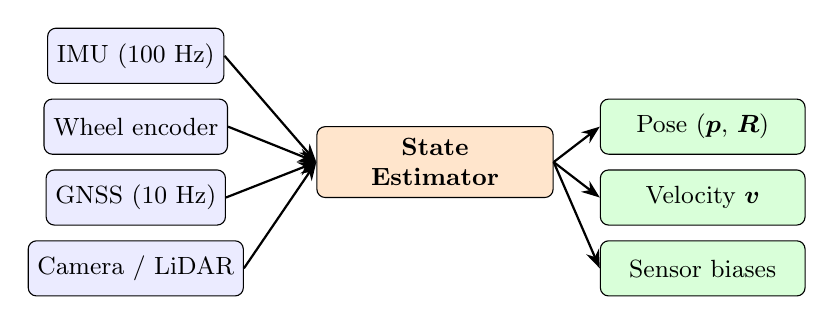
\begin{tikzpicture}[
    sensor/.style={draw, rounded corners=3pt, fill=blue!8,
                   minimum width=2.2cm, minimum height=0.7cm, font=\small},
    fuse/.style={draw, rounded corners=3pt, fill=orange!20,
                 minimum width=3.0cm, minimum height=0.9cm,
                 font=\small\bfseries, align=center},
    outbox/.style={draw, rounded corners=3pt, fill=green!15,
                minimum width=2.6cm, minimum height=0.7cm, font=\small},
    arr/.style={-Stealth, thick}
  ]
    \node[sensor] (imu)  at (0, 1.8)  {IMU (100 Hz)};
    \node[sensor] (enc)  at (0, 0.9)  {Wheel encoder};
    \node[sensor] (gps)  at (0, 0.0)  {GNSS (10 Hz)};
    \node[sensor] (cam)  at (0,-0.9)  {Camera / LiDAR};

    \node[fuse]   (filt) at (3.8, 0.45) {State\\Estimator};

    \node[outbox](pose) at (7.2, 0.9)  {Pose ($\bm{p},\,\bm{R}$)};
    \node[outbox](vel)  at (7.2, 0.0)  {Velocity $\bm{v}$};
    \node[outbox](bias) at (7.2,-0.9)  {Sensor biases};

    \draw[arr] (imu.east)  -- (filt.west);
    \draw[arr] (enc.east)  -- (filt.west);
    \draw[arr] (gps.east)  -- (filt.west);
    \draw[arr] (cam.east)  -- (filt.west);
    \draw[arr] (filt.east) -- (pose.west);
    \draw[arr] (filt.east) -- (vel.west);
    \draw[arr] (filt.east) -- (bias.west);
  \end{tikzpicture}
  \end{center}
  \vspace{0.2em}
  \footnotesize 각 센서의 장점은 취하고 단점은 다른 센서로 보완 — 이것이 fusion의 본질
\end{frame}

% ---------- 4
\begin{frame}{2025년 기준 State Estimation 생태계 지형도}
  \begin{center}
  \begin{tikzpicture}[scale=0.92, transform shape,
    box/.style={draw, rounded corners=4pt, minimum width=4.8cm,
                minimum height=4.2cm, align=center},
    item/.style={font=\footnotesize},
    hl/.style={draw, rounded corners=3pt, fill=orange!30,
               font=\footnotesize\bfseries, inner sep=4pt}
  ]
    % Filter column
    \node[box, fill=blue!6] (fcol) at (0,0) {};
    \node[font=\small\bfseries, blue!70!black] at (0, 1.7) {Filter 계열 (온라인)};
    \node[item] at (0, 1.1)  {KF — 선형 시스템};
    \node[item] at (0, 0.6)  {EKF — 1차 선형화};
    \node[hl]              at (0, 0.0)  {ESKF  ←  이 강의};
    \node[item] at (0,-0.5)  {UKF — Sigma Points};
    \node[item] at (0,-1.1)  {Particle Filter};
    \node[item, gray] at (0,-1.6) {\textit{실시간, 메모리 고정}};

    % Smoother column
    \node[box, fill=green!6] (scol) at (5.6,0) {};
    \node[font=\small\bfseries, green!50!black] at (5.6, 1.7) {Smoother 계열 (오프라인)};
    \node[item] at (5.6, 1.1)  {Factor Graph};
    \node[item] at (5.6, 0.6)  {GTSAM, g2o, Ceres};
    \node[item] at (5.6, 0.0)  {Bundle Adjustment};
    \node[item] at (5.6,-0.5)  {iSAM2 (증분 스무더)};
    \node[item] at (5.6,-1.1)  {Loop Closure / SLAM};
    \node[item, gray] at (5.6,-1.6) {\textit{정밀도 우선, 루프 클로져}};

    % Arrow between
    \draw[-Stealth, dashed, thick, gray]
      (fcol.east) -- (scol.west)
      node[midway, above, font=\scriptsize] {odometry};
  \end{tikzpicture}
  \end{center}
\end{frame}

% ---------- 5
\begin{frame}{Filter vs. Smoother — 언제 뭘 쓰나}
  \footnotesize
  \begin{columns}[T]
    \begin{column}{0.48\textwidth}
      \textbf{\color{blue!70!black} Filter (ESKF 등)}
      \begin{itemize}
        \item 현재 시점까지의 측정만 사용
        \item 고정된 메모리, 고정된 연산량
        \item 실시간 제어 출력에 적합
        \item \textbf{실무 예}: 드론 자세 제어, 자율주행 odometry
      \end{itemize}
    \end{column}
    \begin{column}{0.48\textwidth}
      \textbf{\color{green!50!black} Smoother (Factor Graph 등)}
      \begin{itemize}
        \item 과거 측정을 재사용해 전체 최적화
        \item 메모리·연산이 시간에 비례 증가
        \item 루프 클로져, 정밀 지도 생성에 적합
        \item \textbf{실무 예}: SLAM, SfM, 오프라인 재처리
      \end{itemize}
    \end{column}
  \end{columns}
  \vspace{0.8em}
  \begin{block}{실제 시스템의 구조}
    \textbf{Filter (ESKF)} $\xrightarrow{\text{odometry}}$ \textbf{Smoother (Factor Graph)}\\
    빠른 odometry가 SLAM의 초기값을 공급하는 2계층 구조가 표준
  \end{block}
\end{frame}

% ---------- 6
\begin{frame}{ESKF — 왜 지금 이것인가}
  \textbf{Error-State Kalman Filter (ESKF)}는 실시간 IMU 기반 fusion의 \textbf{사실상 표준}이다.

  \vspace{0.6em}
  \begin{columns}[T]
    \begin{column}{0.52\textwidth}
      \textbf{오픈소스 레퍼런스 구현 (ESKF/iEKF)}
      \begin{itemize}\footnotesize
        \item \textbf{OpenVINS} (U.\ Delaware, 2020)\\
              Visual-Inertial Odometry, MSCKF + ESKF error-state
        \item \textbf{ROVIO} (ETH, 2017)\\
              VIO, IEKF on manifold
        \item \textbf{FAST-LIO2} (HKU MARS, 2022)\\
              LiDAR-IMU odometry, IEKF on SO(3)
        \item \textbf{FAST-LIVO2} (HKU MARS, 2024)\\
              LiDAR + Visual + Inertial, IEKF
      \end{itemize}
      \scriptsize 인접 영역 (factor graph + preintegration):
      VINS-Mono, ORB-SLAM3 VI, LIO-SAM, Kalibr (batch).
    \end{column}
    \begin{column}{0.44\textwidth}
      \textbf{UKF 대비 ESKF의 장점}
      \begin{itemize}\footnotesize
        \item Sigma point 불필요\\
              연산량 동일 또는 적음
        \item 쿼터니언 부호 문제 \textbf{구조적 소멸}
        \item IMU 적분에 최적화된 설계
        \item 수많은 레퍼런스 코드
      \end{itemize}
    \end{column}
  \end{columns}
\end{frame}

% ---------- 7
\begin{frame}{ESKF의 핵심 아이디어 — 미리보기}
  \begin{center}
  \begin{tikzpicture}[
    state/.style={draw, rounded corners, minimum width=3.2cm,
                  minimum height=0.8cm, font=\small, align=center},
    arr/.style={-Stealth, thick}
  ]
    \node[state, fill=blue!10]   (nom) at (0,0)    {Nominal state $\hatx$\\(비선형 적분)};
    \node[state, fill=orange!20] (err) at (5.5,0)  {Error state $\dxvec$\\(선형 KF)};
    \node[state, fill=green!15]  (true) at (2.75,-1.8) {True state $\bm{x}$\\$= \hatx \oplus \dxvec$};

    \draw[arr] (nom.east) -- node[above, font=\scriptsize]{항상 작음} (err.west);
    \draw[arr] (nom.south) -- (true.west);
    \draw[arr] (err.south) -- (true.east);

    \node[font=\footnotesize, align=center] at (2.75, 0.7)
      {측정 후: $\hatx \leftarrow \hatx \oplus \hat{\dxvec}$, \; $\dxvec \leftarrow 0$ (reset)};
  \end{tikzpicture}
  \end{center}
  \vspace{0.3em}
  \footnotesize
  Error state $\dxvec$가 \emph{항상 작다}는 것이 보장되므로 선형 KF를 안전하게 적용 가능
\end{frame}

% ---------- 8
\begin{frame}[shrink=10]{전체 로드맵 — Modern Robot State Estimation}
  \begin{center}
  \footnotesize
  \begin{tabular}{cll}
    \toprule
    강의 & 주제 & 핵심 내용 \\
    \midrule
    0 & 오리엔테이션 & 생태계 지형도, ESKF 위치 설정 \\
    1 & Bayes 필터   & 확률, 가우시안, predict/update, posterior $\to$ next prior \\
    2 & SO(3) 입문 + Jacobians & 매니폴드, Exp/Log, BCH, $J_r/J_l$, Adjoint \\
    3 & 선형 KF      & 5줄 유도, Joseph form, 수치 안정성 \\
    \midrule
    \textbf{4} & \textbf{ESKF 핵심} & \textbf{nominal/error 분리, F matrix, inject \& reset} \\
    5 & IMU + Predict + Preintegration & specific force, F/G 유도, Forster 2017 bias Jac. \\
    6 & 멀티센서 update & GPS/wheel/camera H matrix 유도 \\
    \midrule
    7 & 관측가능성 + Factor Graph + MAP & NIS, GN/LM, Schur, Marginalization, iSAM2 \\
    8 & MSCKF + VIO    & Stochastic cloning, null-space proj., FEJ, OpenVINS \\
    9 & LiDAR 상태 추정 & FAST-LIO/2, ikd-tree, FAST-LIVO/2 \\
    \bottomrule
  \end{tabular}
  \end{center}
  \vspace{0.3em}
  \footnotesize 4강이 전체의 핵심. 1--3강은 수학적 토대, 7--9강은 ESKF를 넘어선 현대 robotics state estimation.
\end{frame}

% ---------- 9
\begin{frame}{필요한 수학 배경}
  \begin{columns}[T]
    \begin{column}{0.48\textwidth}
      \textbf{이미 알면 좋은 것}
      \begin{itemize}\footnotesize
        \item 선형대수 (행렬 곱, 역행렬, 고유값)
        \item 확률론 기초 (가우시안, 조건부 확률)
        \item 미적분 (편미분, 연쇄 법칙)
        \item 쿼터니언 (개념 수준이면 충분)
      \end{itemize}
    \end{column}
    \begin{column}{0.48\textwidth}
      \textbf{이 강의에서 가르치는 것}
      \begin{itemize}\footnotesize
        \item \textbf{Bayes 필터} (1강)
        \item \textbf{SO(3) 매니폴드} (2강)
        \item \textbf{Kalman Filter 유도} (3강)
        \item \textbf{ESKF 전체 구조} (4강)
      \end{itemize}
    \end{column}
  \end{columns}
  \vspace{0.8em}
  \begin{block}{이 강의의 약속}
    이 코스가 끝나면 OpenVINS의 \texttt{Propagator.cpp}/\texttt{UpdaterHelper.cpp},
    그리고 FAST-LIO2의 IEKF 구현을 \emph{한 줄씩 읽고 왜 이렇게 짰는지 설명}할 수 있다.
  \end{block}
\end{frame}

% ---------- 10
\begin{frame}{참고 자료}
  \begin{itemize}
    \item \textbf{Solà et al., ``A micro Lie theory'' (2018)} — SO(3), ESKF 바이블\\
          \texttt{arXiv:1812.01537}
    \item \textbf{Barfoot, ``State Estimation for Robotics'' (2017)} — 교과서 표준
    \item \textbf{Geneva et al., ``OpenVINS'' (ICRA 2020)} — MSCKF + ESKF error-state VIO\\
          \texttt{github.com/rpng/open\_vins}
    \item \textbf{Qin et al., ``VINS-Mono'' (T-RO 2018)} — 드론 VIO (sliding-window factor graph + IMU preintegration)
    \item \textbf{Xu \& Zhang, ``FAST-LIO2'' (T-RO 2022)} — iEKF on manifold, LiDAR-IMU 표준
    \item \textbf{Forster et al., ``IMU Preintegration'' (RSS 2015)} — Factor graph 브리지
    \item \textbf{Bell \& Cathey (IEEE TAC 1993)} — IEKF $\equiv$ Gauss-Newton 등치성 증명
  \end{itemize}
\end{frame}

% ---------- 11 — 0회차 → 1회차 다리
\begin{frame}{다음 회차 예고: 1회차 — Bayes 정리에서 KF가 흘러나오는 모습}
  \begin{block}{한 줄 질문}
    \large
    \emph{여러 센서를 ``확률적으로 결합''한다는 것은 정확히 무슨 뜻인가?}
  \end{block}

  \pause
  \vspace{0.3em}
  \begin{exampleblock}{1회차에서 답할 것}
    \begin{itemize}
      \item Bayes 정리 두 줄 유도 — $p(\bx \mid \bz) \propto p(\bz \mid \bx)\,p(\bx)$
      \item 가우시안 곱 = 평균/분산의 \textbf{가중합} → 이게 KF의 update 그 자체
      \item \alert{Posterior가 다음 턴의 prior가 되는 재귀} — ``filter''라는 개념의 본질
      \item 톱니파(sawtooth) 분산 패턴 — predict가 늘리고 update가 줄임
    \end{itemize}
  \end{exampleblock}

  \pause
  \vspace{0.3em}
  \begin{center}\small\itshape
    \color{gray}
    1회차가 끝나면 KF의 ``5줄''이 어디서 나오는지 머릿속에 그림이 그려진다.\\
    그게 3회차 선형 KF, 4회차 ESKF의 기반이 된다.
  \end{center}
\end{frame}

% =================================
\section{1회차: Bayes filter, Gaussian}
% ---------- 1


% ---------- 2
\begin{frame}{지난 시간 한 줄}
  \begin{center}
    \large
    어떤 단일 센서도 충분치 않다.\\
    \textbf{확률적으로 결합}하는 알고리즘이 필요하다.
  \end{center}
  \vspace{0.6em}
  오늘의 목표:
  \begin{itemize}
    \item 확률, 가우시안, Bayes 정리 — 손에 익히기
    \item Bayes 정리에서 \emph{필연}적으로 \textbf{predict / update} 두 단계가 흘러나오는 모습
    \item 1D 가우시안 곱 — 손으로 한 번, Python으로 한 번
  \end{itemize}
\end{frame}

% ---------- 3
\begin{frame}{용어 정리: 우리가 다루는 것은 모두 \emph{불확실}하다}
  \begin{itemize}
    \item state $\bx$: 알고 싶은 양 (위치, 속도, bias 등)
    \item measurement $\bz$: 센서가 알려주는 양
    \item 둘 다 \emph{확정값}이 아니라 \textbf{확률분포}로 다룬다
  \end{itemize}
  \vspace{0.5em}
  \pause
  \begin{block}{이 코스의 표기}
    ``$\bx$의 belief (믿음)'' = $p(\bx)$ \\
    ``$\bz$를 관측한 뒤 $\bx$의 belief'' = $p(\bx \mid \bz)$
  \end{block}
\end{frame}

% ---------- 4
\begin{frame}{확률의 두 가지 해석}
  \footnotesize
  \begin{itemize}
    \item \textbf{Frequentist:} ``동전을 무한히 던지면 앞면 비율이 0.5''
    \item \textbf{Bayesian:} ``이 동전이 앞면일 거라는 \emph{내 믿음}이 0.5''
  \end{itemize}
  \pause
  \vspace{0.4em}
  \begin{block}{로봇 state estimation에서는?}
    당연히 \textbf{Bayesian}. \\
    ``지금 내 로봇 위치''를 무한히 반복할 수 없다. \\
    우리는 단 한 번의 실현(이 로봇, 이 시점)에 대한 \emph{믿음}을 다룬다.
  \end{block}
\end{frame}

% ---------- 5
\begin{frame}{조건부 확률 — 한 번에 정리}
  \[
    p(A \mid B) \;=\; \frac{p(A, B)}{p(B)}
  \]
  \begin{itemize}
    \item ``$B$가 일어났다는 사실을 알 때, $A$의 확률''
    \item joint $p(A,B)$를 $B$의 \emph{단면}으로 정규화한 것
    \item 이 정의 한 줄로부터 \textbf{Bayes 정리}와 \textbf{전확률 공식}이 모두 따라옴
  \end{itemize}
\end{frame}

% ---------- 6
\begin{frame}{Bayes 정리 — 단 두 줄로 유도}
  $p(A,B) = p(A \mid B)\, p(B) = p(B \mid A)\, p(A)$ 이므로
  \[
    \boxed{\;p(A \mid B) \;=\; \frac{p(B \mid A)\, p(A)}{p(B)}\;}
  \]
  \pause
  \vspace{0.4em}
  state estimation 표기로 바꾸면
  \[
    p(\bx \mid \bz) \;=\; \frac{p(\bz \mid \bx)\, p(\bx)}{p(\bz)}
  \]
  \begin{itemize}
    \item $p(\bx)$: \textbf{prior} — 측정 전 믿음
    \item $p(\bz \mid \bx)$: \textbf{likelihood} — 센서 모델
    \item $p(\bx \mid \bz)$: \textbf{posterior} — 측정 후 믿음
    \item $p(\bz)$: 정규화 상수, 사실상 \emph{곱셈}으로 취급
  \end{itemize}
\end{frame}

% ---------- 7
\begin{frame}{왜 \emph{비례식}으로 충분한가}
  \[
    p(\bx \mid \bz) \;\propto\; p(\bz \mid \bx)\, p(\bx)
  \]
  \begin{itemize}
    \item $p(\bz)$는 $\bx$에 의존하지 않는다 — $\bx$ 변화에 따라 모양이 바뀌지 않음
    \item 마지막에 분포 전체를 적분=1로 맞추면 자동 회복
    \item 그래서 \emph{모양}만 보면 \textbf{prior $\times$ likelihood}가 곧 posterior
  \end{itemize}
  \pause
  \vspace{0.3em}
  \begin{block}{직관 한 줄}
    ``사전 믿음을 측정값이 \emph{얼마나 그럴듯하게} 만드는지로 가중한다.''
  \end{block}
\end{frame}

% ---------- 7.5 — Bayes rule 철학적 요약
\begin{frame}{Bayes 정리 — 엔지니어링 관점의 두 가지 핵심}
  로봇 state estimation을 하는 사람에게 Bayes 정리는 두 줄로 요약된다.

  \vspace{0.6em}
  \begin{block}{\#1 — Posterior는 prior와 observation의 \emph{가중 결합}}
    \[
      \underbrace{p(\bx \mid \bz)}_{\text{posterior}}
      \;\propto\;
      \underbrace{p(\bz \mid \bx)}_{\text{observation}}
      \;\cdot\;
      \underbrace{p(\bx)}_{\text{prior}}
    \]
    가우시안이 되면 이것은 곧 \textbf{평균의 가중합}, 가중치는 정밀도(분산의 역수)이다.\\
    KF의 갱신식 $\hatx^+ = \hatx^- + \bK(\bz - \bH\hatx^-)$가 정확히 이 형태다.
  \end{block}

  \pause
  \vspace{0.4em}
  \begin{alertblock}{\#2 — Posterior는 다음 턴의 prior가 된다 \emph{(이게 더 중요)}}
    \[
      p(\bx_t \mid \bz_{1:t}) \;\xrightarrow{\;\;\text{predict}\;\;}\;
      p(\bx_{t+1} \mid \bz_{1:t}) \;\xrightarrow{\;\;\text{update}\;\;}\;
      p(\bx_{t+1} \mid \bz_{1:t+1})
    \]
    \emph{한 번}만 결합하는 것이 아니라 \textbf{무한 재귀}로 결합한다.\\
    이 재귀가 ``filter''라는 개념의 본질 — 시간을 따라 belief가 \emph{흐른다}.
  \end{alertblock}
\end{frame}

% ---------- 8
\begin{frame}{왜 하필 가우시안인가 — 닫힌 형식의 선택}
  \begin{itemize}
    \item \textbf{중심극한정리}: 독립 잡음의 합 → 가우시안 (실제 센서 잡음의 좋은 근사)
    \item \textbf{닫힌 형식}: 가우시안끼리 곱해도 \emph{또 가우시안}
    \item \textbf{선형 변환}에 닫혀있음: $\bx \sim \Norm{\bm{\mu}}{\bm{\Sigma}}$이면
          $\bA\bx \sim \Norm{\bA\bm{\mu}}{\bA\bm{\Sigma}\bA^\top}$
    \item 평균 + 공분산 두 모멘트만으로 완전히 기술 — \textbf{메모리 효율}
  \end{itemize}
  \pause
  \vspace{0.5em}
  \begin{alertblock}{주의}
    가우시안은 \emph{닫힌 형식이 가능한} 선택이지 \emph{유일한} 선택이 아니다.\\
    비가우시안 문제(다봉 분포, 심한 비선형) → \textbf{Particle filter}가 일반 해.\\
    이 코스는 가우시안으로 제한하되, 그 한계를 명확히 인식하고 넘어간다.
  \end{alertblock}
\end{frame}

% ---------- 9
\begin{frame}{1D 가우시안 — 식과 그림}
  \[
    \mathcal{N}(x;\mu,\sigma^2) \;=\; \frac{1}{\sqrt{2\pi}\,\sigma}\exp\!\left(-\tfrac{(x-\mu)^2}{2\sigma^2}\right)
  \]
  \begin{center}
  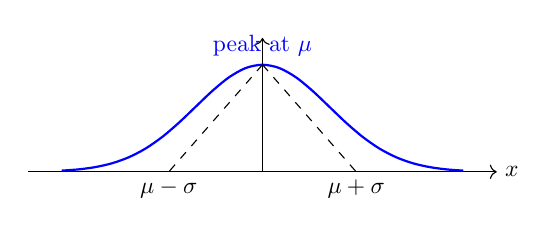
\begin{tikzpicture}[scale=0.85, transform shape]
    \draw[->] (-3.5,0) -- (3.5,0) node[right]{$x$};
    \draw[->] (0,0) -- (0,2.0);
    \draw[domain=-3:3, smooth, thick, blue] plot (\x, {1.6*exp(-\x*\x/2)});
    \draw[dashed] (0,1.6) -- (-1.4,0) node[below]{$\mu - \sigma$};
    \draw[dashed] (0,1.6) -- ( 1.4,0) node[below]{$\mu + \sigma$};
    \node[blue, above] at (0,1.6) {peak at $\mu$};
  \end{tikzpicture}
  \end{center}
  $\sigma$는 \emph{불확실성 폭}이고, 작아질수록 분포가 뾰족해진다.
\end{frame}

% ---------- 10
\begin{frame}{다변수 가우시안 — 공분산이 모양을 정한다}
  \[
    \mathcal{N}(\bx;\bm{\mu},\bm{\Sigma}) \;=\;
    \frac{1}{\sqrt{(2\pi)^n |\bm{\Sigma}|}}
    \exp\!\left(-\tfrac{1}{2}(\bx-\bm{\mu})^\top \bm{\Sigma}^{-1}(\bx-\bm{\mu})\right)
  \]
  \begin{center}
  \begin{tikzpicture}[scale=0.7, transform shape]
    \begin{scope}[shift={(-4,0)}]
      \draw[->] (-2.5,0) -- (2.5,0); \draw[->] (0,-2) -- (0,2);
      \draw[blue, thick] (0,0) ellipse (1.5 and 1.0);
      \node at (0,-2.3) {$\bm{\Sigma}$ 대각, 등방};
    \end{scope}
    \begin{scope}[shift={(0,0)}]
      \draw[->] (-2.5,0) -- (2.5,0); \draw[->] (0,-2) -- (0,2);
      \draw[blue, thick] (0,0) ellipse (1.8 and 0.7);
      \node at (0,-2.3) {대각, $x$방향 더 큼};
    \end{scope}
    \begin{scope}[shift={(4,0)}]
      \draw[->] (-2.5,0) -- (2.5,0); \draw[->] (0,-2) -- (0,2);
      \draw[blue, thick, rotate=30] (0,0) ellipse (1.8 and 0.7);
      \node at (0,-2.3) {비대각 — 상관관계};
    \end{scope}
  \end{tikzpicture}
  \end{center}
  \footnotesize
  비대각 항(off-diagonal)이 KF의 진짜 힘이 어디서 오는지를 결정한다.
\end{frame}

% ---------- 11
\begin{frame}{핵심 보조 정리: 가우시안 $\times$ 가우시안}
  두 1D 가우시안 $\mathcal{N}(x;\mu_1,\sigma_1^2)$, $\mathcal{N}(x;\mu_2,\sigma_2^2)$의 곱은 다시 가우시안:
  \[
    \mu = \frac{\mu_1/\sigma_1^2 + \mu_2/\sigma_2^2}{1/\sigma_1^2 + 1/\sigma_2^2},
    \qquad
    \frac{1}{\sigma^2} = \frac{1}{\sigma_1^2} + \frac{1}{\sigma_2^2}
  \]
  \pause
  \vspace{0.4em}
  \begin{itemize}
    \item 평균은 \textbf{정밀도(=$1/\sigma^2$) 가중 평균}
    \item 분산은 \textbf{역수의 합}으로 결합 → 항상 둘 중 작은 값보다 \emph{더 작다}
    \item 즉 두 정보를 합치면 \emph{불확실성이 줄어든다}
  \end{itemize}
\end{frame}

% ---------- 12
\begin{frame}{가우시안 곱 — 손으로 유도 (1)}
  \footnotesize
  \[
    \mathcal{N}(\mu_1,\sigma_1^2)\,\mathcal{N}(\mu_2,\sigma_2^2)
    \propto \exp\!\left(-\tfrac{(x-\mu_1)^2}{2\sigma_1^2}-\tfrac{(x-\mu_2)^2}{2\sigma_2^2}\right)
  \]
  \pause
  지수 안을 $x$에 대해 정리:
  \[
    -\tfrac{1}{2}\left[\Bigl(\tfrac{1}{\sigma_1^2}+\tfrac{1}{\sigma_2^2}\Bigr) x^2
      - 2\Bigl(\tfrac{\mu_1}{\sigma_1^2}+\tfrac{\mu_2}{\sigma_2^2}\Bigr)x + \text{const}\right]
  \]
  \pause
  새 분산: \;$1/\sigma^2 = 1/\sigma_1^2 + 1/\sigma_2^2$\\
  새 평균: \;$\mu = \sigma^2 \cdot (\mu_1/\sigma_1^2 + \mu_2/\sigma_2^2)$
\end{frame}

% ---------- 13
\begin{frame}{가우시안 곱 — 손으로 유도 (2)}
  \footnotesize
  대입하면 $\mu$가 정밀도 가중평균 형태로 단순화:
  \[
    \mu = \frac{\mu_1/\sigma_1^2 + \mu_2/\sigma_2^2}{1/\sigma_1^2 + 1/\sigma_2^2}
  \]
  \pause
  \vspace{0.3em}
  \textbf{식의 의미를 다시 보면}
  \begin{itemize}
    \item $\sigma_1 \to 0$: 첫 측정이 완벽 → $\mu \to \mu_1$ (그 값을 그대로 받음)
    \item $\sigma_1 \to \infty$: 첫 측정이 무의미 → $\mu \to \mu_2$ (둘째 값만 사용)
    \item 그 사이는 매끄럽게 보간
  \end{itemize}
\end{frame}

% ---------- 14
\begin{frame}{같은 식, KF 게인 형태로 다시 쓰기}
  \footnotesize
  $K \;=\; \dfrac{\sigma_1^2}{\sigma_1^2 + \sigma_2^2}$ \; 라 하면
  \[
    \mu = \mu_1 + K(\mu_2 - \mu_1), \qquad \sigma^2 = (1-K)\,\sigma_1^2
  \]
  \pause
  \vspace{0.5em}
  \begin{block}{이게 바로 1D Kalman update}
    \begin{itemize}
      \item $\mu_1, \sigma_1^2$: prior
      \item $\mu_2, \sigma_2^2$: 측정
      \item $K$: \textbf{Kalman gain} — ``측정을 얼마나 신뢰할지''
      \item $(\mu_2 - \mu_1)$: \textbf{innovation} — 측정과 예측의 차이
    \end{itemize}
  \end{block}
  3회차에서 이 형태가 다차원으로 그대로 일반화된다.
\end{frame}

% ---------- 15
\begin{frame}{이제 Bayes 정리로 돌아가서 — 시간을 끌어들이자}
  로봇은 \emph{시계열}이다. 시간 $k$의 state $\bx_k$를 추정하고 싶다.
  \vspace{0.4em}
  \begin{itemize}
    \item 두 종류의 정보:
      \begin{enumerate}
        \item \textbf{운동 모델} $p(\bx_k \mid \bx_{k-1})$ — ``이전 상태에서 어떻게 움직였을까''
        \item \textbf{측정 모델} $p(\bz_k \mid \bx_k)$ — ``이 상태일 때 센서가 뭘 보여줄까''
      \end{enumerate}
  \end{itemize}
  \pause
  \vspace{0.3em}
  Bayes 정리를 \emph{시간 순으로} 풀어 적용하면 두 단계가 자연스럽게 분리된다.
\end{frame}

% ---------- 16
\begin{frame}{Bayes filter — predict 단계 유도}
  $\bx_k$의 prior를 이전 posterior로부터 만든다 (전확률 공식):
  \[
    p(\bx_k \mid \bz_{1:k-1}) \;=\;
    \int p(\bx_k \mid \bx_{k-1})\, p(\bx_{k-1} \mid \bz_{1:k-1})\, d\bx_{k-1}
  \]
  \begin{itemize}
    \item 운동 모델 $p(\bx_k \mid \bx_{k-1})$로 ``이전 belief를 \emph{미래로 옮긴다}''
    \item 측정값은 아직 안 들어왔다 — 그래서 \textbf{predict}
    \item 결과로 belief가 \emph{퍼진다}(불확실성 증가) — 직관과 일치
  \end{itemize}
\end{frame}

% ---------- 17
\begin{frame}{Bayes filter — update 단계 유도}
  새 측정 $\bz_k$가 들어오면 Bayes 정리로 갱신:
  \[
    p(\bx_k \mid \bz_{1:k}) \;\propto\;
    p(\bz_k \mid \bx_k)\, p(\bx_k \mid \bz_{1:k-1})
  \]
  \begin{itemize}
    \item likelihood $\times$ prior $\rightarrow$ posterior
    \item 측정이 \emph{좁히는} 효과 — 불확실성 감소
  \end{itemize}
  \pause
  \vspace{0.5em}
  \begin{block}{핵심 메시지}
    \textbf{predict}는 운동 모델로 시간을 흘려보내고, \textbf{update}는 측정으로 분포를 좁힌다. \\
    이 두 단계의 분리는 \emph{선택}이 아니라 Bayes 정리의 \emph{필연}이다.
  \end{block}
\end{frame}

% ---------- 18
\begin{frame}{Bayes filter — 한 슬라이드로}
  \begin{center}
  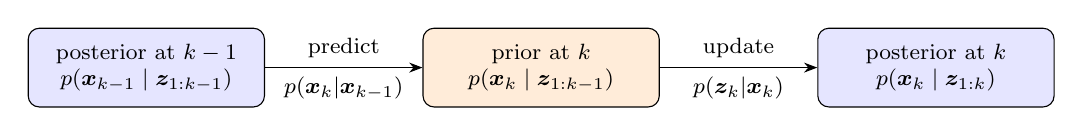
\begin{tikzpicture}[font=\footnotesize, node distance=1.0cm,
    blk/.style={draw, rounded corners, minimum height=1.0cm, minimum width=3.0cm, align=center}]
    \node[blk, fill=blue!10]   (post0) {posterior at $k-1$\\$p(\bx_{k-1} \mid \bz_{1:k-1})$};
    \node[blk, fill=orange!15, right=2.0cm of post0]
                               (pred)  {prior at $k$\\$p(\bx_k \mid \bz_{1:k-1})$};
    \node[blk, fill=blue!10,   right=2.0cm of pred]
                               (post)  {posterior at $k$\\$p(\bx_k \mid \bz_{1:k})$};

    \draw[-Stealth] (post0) -- node[above]{predict}
                              node[below]{$p(\bx_k|\bx_{k-1})$} (pred);
    \draw[-Stealth] (pred)  -- node[above]{update}
                              node[below]{$p(\bz_k|\bx_k)$}     (post);
  \end{tikzpicture}
  \end{center}
  \vspace{0.5em}
  \begin{itemize}
    \item 매 시간 스텝마다 두 박스를 \emph{번갈아} 통과
    \item ESKF의 100\,Hz predict + 비동기 update가 정확히 이 구조
  \end{itemize}
\end{frame}

% ---------- 19
\begin{frame}{Bayes filter는 \emph{완벽}하지만 풀 수 없다}
  \begin{itemize}
    \item predict의 적분 $\int \cdots d\bx_{k-1}$ — 일반적으로 닫힌 해 없음
    \item update의 정규화 $p(\bz)$ — 일반적으로 닫힌 해 없음
    \item state가 연속, 분포 임의 모양이면 \textbf{이론상 가능}하지만 \emph{컴퓨터로 못 풂}
  \end{itemize}
  \pause
  \vspace{0.5em}
  \begin{block}{돌파구}
    \textbf{분포를 가우시안으로 가정}하면 두 단계 모두 닫힌 해가 나온다. \\
    이게 \textbf{Kalman Filter}.
  \end{block}
\end{frame}

% ---------- 20
\begin{frame}{KF는 Bayes filter + 가우시안 가정}
  \begin{itemize}
    \item prior, posterior를 \emph{모두} 가우시안으로 표현
    \item 운동 모델, 측정 모델도 \emph{선형 + 가우시안 잡음}으로 가정
    \item 그러면 두 단계가 \textbf{평균과 공분산의 업데이트}로 환원됨
    \item 식 5줄로 끝 — 3회차에서 정식 유도
  \end{itemize}
  \pause
  \vspace{0.4em}
  \begin{columns}[T]
    \begin{column}{0.48\textwidth}
      \textbf{비선형이면?}\\
      ESKF — 4회차
    \end{column}
    \begin{column}{0.48\textwidth}
      \textbf{비-가우시안이면?}\\
      Particle filter (이 코스 범위 밖)
    \end{column}
  \end{columns}
\end{frame}

% ---------- 21
\begin{frame}{Bayes filter의 가정을 KF로 좁히는 사다리}
  \begin{center}
  \begin{tikzpicture}[font=\footnotesize, node distance=0.4cm,
    blk/.style={draw, rounded corners, minimum width=8cm, minimum height=0.8cm, align=center}]
    \node[blk, fill=red!10]   (a) {일반 Bayes filter (any distribution)};
    \node[blk, fill=orange!12, below=of a] (b) {분포를 가우시안으로 제한};
    \node[blk, fill=yellow!15, below=of b] (c) {모델을 \emph{선형} + 가우시안 잡음으로};
    \node[blk, fill=green!12,  below=of c] (d) {\textbf{Kalman Filter}};
    \draw[-Stealth] (a) -- (b);
    \draw[-Stealth] (b) -- (c);
    \draw[-Stealth] (c) -- (d);
  \end{tikzpicture}
  \end{center}
  \begin{itemize}
    \item 우리는 사다리를 한 칸 한 칸 내려가며 \emph{왜} 그런 가정이 필요한지 추적할 것
    \item 4회차에서 ``비선형''으로 한 단 위로 올라간다 (ESKF)
  \end{itemize}
\end{frame}

% ---------- 22
\begin{frame}{사고실험 — 직선 복도 + 점자블럭}
  \begin{itemize}
    \item state: $x$ (직선 위 위치)
    \item 운동 모델: 한 발 옮기면 $x \leftarrow x + 0.7 + w$, $w \sim \mathcal{N}(0, 0.05^2)$
    \item 측정 모델: 점자가 있는 정확한 1m 지점에서 $z = x + v$, $v \sim \mathcal{N}(0, 0.02^2)$
  \end{itemize}
  \pause
  \vspace{0.3em}
  \begin{itemize}
    \item predict: 매 발걸음마다 $\sigma$가 \emph{커진다}
    \item update: 점자 측정이 들어오면 가우시안 곱 → $\sigma$ 다시 \emph{작아진다}
    \item 두 효과의 균형이 \emph{지속 가능한 추정}을 만든다
  \end{itemize}
\end{frame}

% ---------- 23
\begin{frame}{update — 가우시안 두 개의 곱으로 쓰기}
  \footnotesize
  prior (predict 결과): $\mathcal{N}(x;\, 70,\; 0.25)$ at 100보\\
  measurement (점자 100번째): $\mathcal{N}(x;\, 100,\; 0.0004)$
  \pause
  \vspace{0.3em}
  곱하면:
  \[
    \tfrac{1}{\sigma^2} = \tfrac{1}{0.25}+\tfrac{1}{0.0004} \approx 2504
    \;\;\Rightarrow\;\; \sigma \approx 0.02
  \]
  \[
    \mu = \frac{70/0.25 + 100/0.0004}{2504} \approx 99.99
  \]
  \begin{itemize}
    \item 결과: 분산은 \emph{측정의 분산과 거의 같음}
    \item 직관: 정확한 측정 한 번이 prior를 거의 \emph{덮어쓴다}
  \end{itemize}
\end{frame}

% ---------- 24
\begin{frame}{왜 우리는 \emph{공분산}이라는 행렬을 굳이 쓰는가}
  \footnotesize
  \begin{itemize}
    \item state가 단일 변수라면 분산만 있으면 됨
    \item 그러나 state가 여러 차원이고 \textbf{서로 상관}되어 있으면?
  \end{itemize}
  \pause
  \vspace{0.3em}
  예: 위치 $x$와 속도 $v$
  \[
    \bm{\Sigma} = \begin{pmatrix} \sigma_x^2 & \rho\,\sigma_x\sigma_v \\
                                   \rho\,\sigma_x\sigma_v & \sigma_v^2 \end{pmatrix}
  \]
  \begin{itemize}
    \item $\rho > 0$: ``위치를 더 안다''는 정보가 들어오면 \emph{속도 추정도} 좁아진다
    \item 이 상호작용이 KF의 진짜 힘 — \textbf{한 변수의 측정이 다른 변수까지 좁힌다}
    \item IMU bias 추정이 자동으로 되는 이유도 똑같음 (5회차에서 적용)
  \end{itemize}
\end{frame}

% ---------- 25
\begin{frame}{predict / update 반복 — 분산이 어떻게 움직이나 (sawtooth)}
  \begin{center}
  \begin{tikzpicture}[scale=0.95, transform shape, font=\footnotesize,
    update arrow/.style={red, thick, -Stealth}]
    % axes
    \draw[->] (-0.3,0) -- (10.6,0) node[right]{$t$};
    \draw[->] (0,-0.2) -- (0,3.2) node[above]{$\sigma^2(t)$ \scriptsize (분산)};

    % steady-state asymptote (참고선)
    \draw[gray!50, dashed, thick] (0,1.3) -- (10.4,1.3)
      node[right, gray, font=\scriptsize]{$\sigma^2_\infty$ (steady-state)};

    % --- 톱니파 sawtooth: 초기에 큰 분산 → 점차 정상상태로 수렴 ---
    % cycle 1: predict 0->2 grows, update at 2 drops
    \draw[blue, thick] (0, 0.3) -- (2.0, 1.6);
    \draw[update arrow] (2.0, 1.6) -- (2.0, 0.7);
    \fill[red] (2.0, 1.6) circle (1.6pt);

    % cycle 2: predict 2->4 grows, update at 4 drops
    \draw[blue, thick] (2.0, 0.7) -- (4.0, 1.85);
    \draw[update arrow] (4.0, 1.85) -- (4.0, 1.05);
    \fill[red] (4.0, 1.85) circle (1.6pt);

    % cycle 3: predict 4->6 grows, update at 6 drops
    \draw[blue, thick] (4.0, 1.05) -- (6.0, 1.85);
    \draw[update arrow] (6.0, 1.85) -- (6.0, 1.20);
    \fill[red] (6.0, 1.85) circle (1.6pt);

    % cycle 4: 정상상태 근처
    \draw[blue, thick] (6.0, 1.20) -- (8.0, 1.65);
    \draw[update arrow] (8.0, 1.65) -- (8.0, 1.30);
    \fill[red] (8.0, 1.65) circle (1.6pt);

    % cycle 5: 정상상태
    \draw[blue, thick] (8.0, 1.30) -- (10.0, 1.55);
    \draw[update arrow] (10.0, 1.55) -- (10.0, 1.32);
    \fill[red] (10.0, 1.55) circle (1.6pt);

    % labels
    \node[blue, anchor=south west, font=\scriptsize] at (1.0, 1.0) {predict ($+\bF\bP\bF^\top + \bQ$)};
    \node[red,  anchor=west,        font=\scriptsize] at (4.15, 1.45) {update ($-\bK\bH\bP$)};

    % 초기/정상상태 화살 표시
    \draw[<->, gray!70, font=\scriptsize] (0.1, 2.7) -- node[above]{transient: 초기 빠른 수축} (5.0, 2.7);
    \draw[<->, gray!70, font=\scriptsize] (5.2, 2.7) -- node[above]{steady-state: $P_\infty$} (10.0, 2.7);
  \end{tikzpicture}
  \end{center}

  \begin{columns}[T]
    \begin{column}{0.50\textwidth}
      \scriptsize
      \begin{itemize}
        \item \textbf{파란선}: predict가 분산을 늘림 ($\bP \mapsto \bF\bP\bF^\top + \bQ$)
        \item \textbf{빨간 화살}: update가 분산을 줄임 ($\bP \mapsto (\bI-\bK\bH)\bP$)
        \item \textbf{톱니파(sawtooth)}: 매 사이클 predict↑ $\to$ update↓ 반복
      \end{itemize}
    \end{column}
    \begin{column}{0.48\textwidth}
      \scriptsize
      \begin{itemize}
        \item \textbf{Steady-state}: 관측가능 시스템에서 $\bP \to \bP_\infty$ 수렴 (DARE 해)
        \item \textbf{ESKF 실제 비율}: predict 100--400\,Hz, GPS 1--10\,Hz, camera 10--30\,Hz
        \item update 빈도가 낮을수록 톱니의 진폭이 커짐
      \end{itemize}
    \end{column}
  \end{columns}
\end{frame}

% ---------- 26
\begin{frame}{잠깐 — likelihood vs measurement noise}
  \begin{itemize}
    \item likelihood $p(\bz \mid \bx)$ — 어떤 state일 때 어떤 측정이 나올 \emph{확률}
    \item measurement noise $\bv \sim \Norm{0}{\bR}$ — 그 확률을 \emph{만드는 잡음}
    \item 가우시안 가정에서 둘은 사실상 같은 객체의 두 표현
  \end{itemize}
  \pause
  \vspace{0.4em}
  \begin{block}{practical 메모}
    $\bR$를 너무 작게 잡으면 (``내 센서는 매우 정확해!'') → 노이즈를 \emph{진실}로 받아들여 추정이 진동\\
    $\bR$를 너무 크게 잡으면 → 측정을 거의 무시 → 사실상 dead reckoning
  \end{block}
\end{frame}

% ---------- 27
\begin{frame}[fragile,shrink=10]{1D Bayes filter — Python 구현}
\begin{lstlisting}[language=Python]
import numpy as np

def predict(mu, var, u, q):
    # x_k = x_{k-1} + u + w,  w ~ N(0, q)
    return mu + u, var + q

def update(mu, var, z, r):
    # z = x + v,  v ~ N(0, r)
    K = var / (var + r)       # Kalman gain (1D)
    return mu + K*(z - mu), (1 - K)*var

mu, var = 0.0, 1.0
u, q, r = 0.7, 0.05**2, 0.02**2
for k in range(1, 101):
    mu, var = predict(mu, var, u, q)
    if k % 10 == 0:           # measurement every 10 steps
        mu, var = update(mu, var, k * 1.0, r)
\end{lstlisting}
  \begin{itemize}\footnotesize
    \item \texttt{predict}: 분산 \emph{커짐},\quad \texttt{update}: 분산 \emph{줄어듦}
    \item 측정 주기를 바꾸면($k\%20$, $k\%50$) 분산이 어떻게 달라지는가?
  \end{itemize}
\end{frame}

% ---------- 28
\begin{frame}{이번 회차 핵심 다섯 개}
  \begin{enumerate}
    \item Bayes 정리 한 줄에서 predict/update가 \emph{필연}으로 따라온다
    \item 가우시안 곱 = 정밀도 가중평균 + 정밀도 합
    \item 같은 식을 다시 쓰면 1D Kalman update의 표준 형태
    \item 가우시안은 \emph{닫힌 형식이 가능한} 선택 — 비가우시안은 Particle filter
    \item 공분산의 \emph{비대각}이 한 변수의 측정으로 다른 변수까지 좁히게 만든다
  \end{enumerate}
\end{frame}

% ---------- 29
\begin{frame}{다음 시간 예고 — 2회차: SO(3)와 회전}
  \textbf{회전이라는 매니폴드}
  \begin{itemize}
    \item Euler angle의 특이점(Gimbal lock) — 왜 위험한가
    \item 쿼터니언: 더 낫지만 제약($|\mathbf{q}|=1$)이 있다
    \item \textbf{SO(3)}: 회전 전체가 이루는 공간, 그 tangent space = $\mathfrak{so}(3) \cong \mathbb{R}^3$
    \item Exp / Log map: 회전 벡터와 회전 행렬을 오가는 다리
    \item 왜 이게 ESKF의 핵심인가 — error state가 $\mathfrak{so}(3)$에 산다
  \end{itemize}
  \vspace{0.5em}
  \begin{block}{미니 예고}
    노트북을 $x$축 $90^\circ$ 후 $z$축 $90^\circ$ = $z$축 $90^\circ$ 후 $x$축 $90^\circ$ ?\\
    순서를 바꾸면 결과가 \emph{다르다} — 이게 SO(3)가 벡터 공간이 아닌 이유.
  \end{block}
\end{frame}

% =================================
\section{2회차: SO(3) 입문}
% ---------- 1


% ---------- 2
\begin{frame}{지난 시간 한 줄}
  \begin{center}
    \large
    Bayes filter는 Predict + Update. \\
    가우시안이면 닫힌 형식으로 풀린다 $\rightarrow$ \textbf{KF}.
  \end{center}
  \vspace{0.5em}
  오늘의 목표:
  \begin{itemize}
    \item 회전 표현의 생태계 — 왜 쿼터니언도 완벽하지 않은가
    \item \textbf{SO(3)}: 회전이 이루는 공간의 기하학적 구조
    \item \textbf{tangent space} $\cong \mathbb{R}^3$: 작은 회전은 벡터다
    \item Exp / Log map: 회전 벡터 $\leftrightarrow$ 회전 행렬
    \item 왜 이것이 \textbf{ESKF의 핵심 기반}인가
  \end{itemize}
\end{frame}

% ---------- 3
\begin{frame}{회전 표현의 세 가지 선택지}
  \begin{center}
  \begin{tikzpicture}[
    box/.style={draw, rounded corners, minimum width=3.3cm, minimum height=1.8cm,
                align=center, font=\footnotesize},
    arr/.style={-Stealth, thick}
  ]
    \node[box, fill=red!10]    (euler) at (0,0)
      {\textbf{Euler angles}\\$(r,p,y)$, 3 params\\Gimbal lock!};
    \node[box, fill=yellow!15] (quat)  at (4.4,0)
      {\textbf{Quaternion}\\$\mathbf{q}=(q_w,q_x,q_y,q_z)$\\4 params, $|\mathbf{q}|=1$};
    \node[box, fill=green!12]  (SO3)   at (8.8,0)
      {\textbf{SO(3)}\\$\bm{R}\in\mathbb{R}^{3\times3}$\\9 params, 6 constraints};

    \draw[arr] (euler.east) -- node[above,font=\scriptsize]{특이점 제거} (quat.west);
    \draw[arr] (quat.east)  -- node[above,font=\scriptsize]{기하학 명확} (SO3.west);
  \end{tikzpicture}
  \end{center}
  \vspace{0.5em}
  \begin{itemize}
    \item 어떤 표현도 ``공짜로'' 완벽하지 않음 — 표현마다 장단점이 있다
    \item ESKF는 \textbf{쿼터니언(구현)} + \textbf{SO(3) 기하학(이론)}을 결합
  \end{itemize}
\end{frame}

% ---------- 4
\begin{frame}{Euler angle의 치명적 결함 — Gimbal lock}
  Roll-Pitch-Yaw 표현에서 pitch = 90°이면:
  \begin{itemize}\footnotesize
    \item $x$축 회전과 $z$축 회전이 \emph{같은 방향}을 가리킴 $\rightarrow$ DOF 소실
    \item 미분을 구하면 행렬식 $= 0$ $\rightarrow$ \textbf{Jacobian 특이}
    \item KF의 F, H matrix가 수치적으로 폭발
    \item 실제 사례: 아폴로 11호 짐벌 잠김, 비행기 자세 추정 오류
  \end{itemize}
  \pause
  \vspace{0.5em}
  \begin{block}{결론}
    회전을 미분 가능한 형태로 다루는 estimation 문제에서\\
    Euler angle은 원천적으로 사용할 수 없다.
  \end{block}
\end{frame}

% ---------- 5
\begin{frame}{쿼터니언 — 더 낫지만 제약이 있다}
  $\mathbf{q} = (q_w,\, q_x,\, q_y,\, q_z)$, \quad $|\mathbf{q}|=1$ (단위 쿼터니언)
  \vspace{0.4em}
  \begin{itemize}
    \item \textbf{장점}: Gimbal lock 없음, 회전 합성은 단순 곱
    \item \textbf{회전 표현}: 축 $\hat{\mathbf{n}}$, 각 $\theta$ $\Rightarrow$
          $\mathbf{q} = \bigl(\cos\tfrac{\theta}{2},\; \hat{\mathbf{n}}\sin\tfrac{\theta}{2}\bigr)$
    \item \textbf{단점}: $\mathbf{q}$와 $-\mathbf{q}$가 같은 회전 표현 (double-cover)
  \end{itemize}
  \vspace{0.3em}
  \scriptsize
  \alert{표기 주의}: 이 코스는 \textbf{Hamilton 컨벤션 $(q_w, q_x, q_y, q_z)$} 사용 — Eigen, GTSAM, ROS \texttt{tf2}와 일치.\\
  OpenVINS는 \textbf{JPL 컨벤션 $(q_x, q_y, q_z, q_w)$} 사용 — 코드 인용 시 변환 필요 (5/8회차에서 명시).
  \pause
  \vspace{0.4em}
  \begin{alertblock}{KF에서 쿼터니언의 문제}
    KF는 상태를 \emph{벡터}로 다룬다.\\
    $\hat{\mathbf{q}} + K\nu$로 갱신 $\rightarrow$ $|\mathbf{q}|\neq 1$이 될 수 있다.\\
    단순 renormalize를 하면 공분산이 잘못된 방향을 가리킨다.
  \end{alertblock}
\end{frame}

% ---------- 6
\begin{frame}{SO(3) — 3D 회전의 집합 그 자체}
  \[
    \SOthree \;=\; \bigl\{\, \bm{R} \in \mathbb{R}^{3\times3} \;\big|\;
    \bm{R}^\top\bm{R} = \bm{I},\; \det(\bm{R}) = +1 \,\bigr\}
  \]
  \begin{itemize}
    \item 6개의 제약으로 $\mathbb{R}^{9}$ 안에서 \textbf{3차원 면(manifold)}이 된다
    \item 이 면 위의 각 점 = 하나의 3D 회전
    \item 두 회전의 합성: 행렬 곱 $\bm{R}_1\bm{R}_2$ (닫혀있음)
    \item 항등원: $\bm{I}$, \quad 역원: $\bm{R}^\top$
    \item \textbf{군(group)} + 미분 가능한 면 $\rightarrow$ \textbf{Lie group}
  \end{itemize}
\end{frame}

% ---------- 7
\begin{frame}{매니폴드 직관 — 구면으로 생각하기}
  \begin{columns}[T]
    \begin{column}{0.55\textwidth}
      \footnotesize
      지구 표면을 생각하자:
      \begin{itemize}
        \item 전체 공간: $\mathbb{R}^3$ (3D)
        \item 지구 표면: $\mathbb{R}^3$에 박힌 \textbf{2D 면} $= S^2$
        \item 한 점에서 아주 \emph{작은} 이동은 \textbf{평면}처럼 느껴진다
        \item 그 ``국소 평면'' = \textbf{tangent space}
      \end{itemize}
      \vspace{0.4em}
      SO(3)도 마찬가지:
      \begin{itemize}
        \item $\mathbb{R}^9$ 안의 3D 면
        \item 한 회전 $\bm{R}$ 근방의 작은 변화\\
              $\rightarrow$ tangent space $\cong \mathbb{R}^3$
      \end{itemize}
    \end{column}
    \begin{column}{0.42\textwidth}
      \begin{center}
      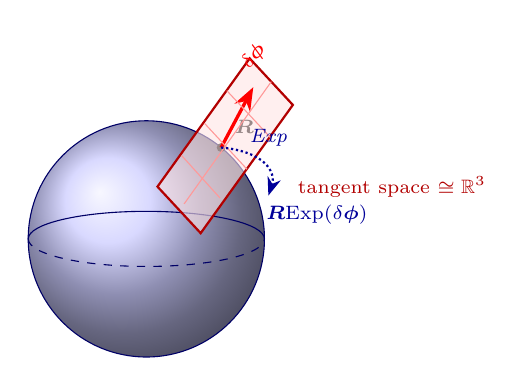
\begin{tikzpicture}[scale=1.0, transform shape, font=\scriptsize]
        % --- Sphere ---
        \shade[ball color=blue!20] (0,0) circle (1.5cm);
        % equator (back half dashed, front half solid for 3D feel)
        \draw[blue!40!black, dashed, thin] (-1.5,0) arc (180:360:1.5cm and 0.35cm);
        \draw[blue!40!black, thin]         (-1.5,0) arc (180:0:1.5cm and 0.35cm);
        % outline (top half)
        \draw[blue!40!black, thin] (0,0) circle (1.5cm);

        % --- Tangent point R (top-right of sphere) ---
        % point on sphere surface
        \coordinate (R) at (0.95, 1.16);
        \fill[black] (R) circle (1.6pt);
        \node[anchor=south west, font=\scriptsize] at ($(R)+(0.05,0.05)$) {$\bm{R}$};

        % --- Normal direction (for tilting tangent plane) ---
        % tangent plane: parallelogram in proper perspective at R, perpendicular to OR
        % outward normal direction at R is along (R - O)
        % Use rotation: plane spans two tangent directions
        % approx tangent basis at R = (0.95, 1.16): t1 = (-1.16, 0.95)/norm (in plane of page),
        % t2 ≈ small "into-page" direction shown as compressed
        \begin{scope}[shift={(R)}, rotate=50]
          % Parallelogram (tilted to look like a tangent plane in 3D)
          \fill[red!10, opacity=0.6]
            (-1.0,-0.5) -- (1.0,-0.35) -- (1.1,0.45) -- (-0.9,0.30) -- cycle;
          \draw[red!70!black, thick]
            (-1.0,-0.5) -- (1.0,-0.35) -- (1.1,0.45) -- (-0.9,0.30) -- cycle;
          % delta-phi vector lying IN the plane
          \draw[-Stealth, red, very thick] (0,0) -- (0.85, 0.18)
                node[anchor=south west, font=\scriptsize, red]{$\delta\bm{\phi}$};
          % small grid in plane (hint of flatness)
          \draw[red!40, thin] (-0.5, -0.40) -- (-0.4, 0.32);
          \draw[red!40, thin] ( 0.0, -0.43) -- ( 0.1, 0.36);
          \draw[red!40, thin] ( 0.5, -0.40) -- ( 0.6, 0.41);
          \draw[red!40, thin] (-0.85, -0.10) -- (1.05, 0.05);
        \end{scope}
        \node[red!70!black, font=\scriptsize, anchor=west]
              at ($(R)+(0.85,-0.50)$) {tangent space $\cong \mathbb{R}^3$};

        % --- Exp map curve: arc from R along the sphere surface ---
        \draw[-Stealth, blue!60!black, thick, densely dotted]
          (R) .. controls ($(R)+(0.55,-0.05)$) and (1.65,0.85) .. (1.55, 0.55);
        \node[blue!60!black, font=\scriptsize, anchor=north west]
              at (1.40, 0.55) {$\bm{R}\Exp(\delta\bm{\phi})$};
        \node[blue!60!black, font=\scriptsize, anchor=south]
              at (1.55, 1.05) {\itshape Exp};
      \end{tikzpicture}
      \end{center}
      \scriptsize
      \begin{itemize}
        \item[\textcolor{red}{$\bullet$}] 빨간 평면 = $\bm{R}$ 점에서의 tangent space
        \item[\textcolor{blue!60!black}{$\bullet$}] 점선 곡선 = $\Exp$ map (평면 → 구면)
      \end{itemize}
    \end{column}
  \end{columns}
\end{frame}

% ---------- 8
\begin{frame}{Lie algebra $\sothree$ — tangent space at identity}
  $\bm{R} = \bm{I}$ 근방에서 SO(3)의 tangent space를 \textbf{Lie algebra}라 부른다:
  \[
    \sothree \;=\; \bigl\{\, \bm{\Phi} \in \mathbb{R}^{3\times3} \;\big|\;
    \bm{\Phi} + \bm{\Phi}^\top = \bm{0} \,\bigr\}
    \quad \text{(반대칭 행렬)}
  \]
  \pause
  \vspace{0.3em}
  반대칭 행렬은 \textbf{3개의 자유 파라미터}만 가진다:
  \[
    \skewx{\bm{\phi}} \;=\;
    \begin{pmatrix} 0 & -\phi_z & \phi_y \\ \phi_z & 0 & -\phi_x \\ -\phi_y & \phi_x & 0 \end{pmatrix},
    \quad \bm{\phi} = (\phi_x, \phi_y, \phi_z)^\top \in \mathbb{R}^3
  \]
  \pause
  \vspace{0.3em}
  \begin{block}{핵심}
    $\sothree \cong \mathbb{R}^3$. \quad
    작은 회전 $\delta\bm{R} \approx \bm{I}$는 \textbf{3D 벡터} $\bm{\phi}$로 기술된다. \\
    ESKF에서 rotation error state $\dphivec \in \mathbb{R}^3$가 등장하는 이유가 바로 이것.
  \end{block}
\end{frame}

% ---------- 9
\begin{frame}{Exponential map — 벡터를 회전으로}
  \[
    \Exp(\bm{\phi}) \;:=\; e^{\skewx{\bm{\phi}}} \;=\;
    \bm{I} + \frac{\sin\|\bm{\phi}\|}{\|\bm{\phi}\|}\,\skewx{\bm{\phi}}
    + \frac{1-\cos\|\bm{\phi}\|}{\|\bm{\phi}\|^2}\,\skewx{\bm{\phi}}^2
  \]
  (Rodrigues 공식)
  \vspace{0.4em}
  \begin{itemize}
    \item 입력: $\bm{\phi} \in \mathbb{R}^3$ (방향 = 회전축, 크기 = 각도)
    \item 출력: $\bm{R} \in \SOthree$
    \item $\|\bm{\phi}\| \to 0$이면 $\Exp(\bm{\phi}) \approx \bm{I} + \skewx{\bm{\phi}}$ (1차 근사)
  \end{itemize}
  \pause
  \vspace{0.3em}
  \textbf{예시}: $\bm{\phi} = (0, 0, \pi/2)^\top$ $\rightarrow$ $z$축 중심 90° 회전:
  \[
    \Exp\!\begin{pmatrix}0\\0\\\pi/2\end{pmatrix} =
    \begin{pmatrix}0 & -1 & 0 \\ 1 & 0 & 0 \\ 0 & 0 & 1\end{pmatrix}
  \]
\end{frame}

% ---------- 10
\begin{frame}{Logarithm map — 회전을 벡터로}
  $\Exp$의 역:
  \[
    \Log(\bm{R}) \;=\; \frac{\theta}{2\sin\theta}\,(\bm{R} - \bm{R}^\top)^\vee,
    \qquad \theta = \arccos\!\Bigl(\tfrac{\mathrm{tr}(\bm{R})-1}{2}\Bigr)
  \]
  여기서 $(\cdot)^\vee$: 반대칭 행렬에서 3D 벡터 추출 ($\skewx{\cdot}$의 역)
  \vspace{0.4em}
  \begin{itemize}
    \item 출력: $\bm{\phi} \in \mathbb{R}^3$, \quad $\|\bm{\phi}\| \in [0, \pi]$
    \item $\Exp$와 $\Log$는 서로 역함수
    \item $\theta = \pi$에서 불연속 — 실제 시스템에서 피해야 할 조건
  \end{itemize}
  \pause
  \begin{block}{요약}
    \begin{center}
    $\mathbb{R}^3 \;\xrightarrow{\;\Exp\;}\; \SOthree \;\xrightarrow{\;\Log\;}\; \mathbb{R}^3$
    \end{center}
    두 공간을 ``사다리''처럼 오간다.
  \end{block}
\end{frame}

% ---------- 11
\begin{frame}{Perturbation — 회전의 ``덧셈''}
  SO(3)에서 기준 회전 $\hatR$ 주변의 작은 변화를 표현하는 방법:
  \vspace{0.4em}
  \textbf{오른쪽 섭동 (right perturbation):}
  \[
    \bm{R} = \hatR\, \Exp(\dphivec) \approx \hatR\,(\bm{I} + \skewx{\dphivec})
  \]
  \pause
  \vspace{0.3em}
  \begin{itemize}
    \item $\dphivec \in \mathbb{R}^3$ — \textbf{제약 없는 벡터}, KF로 추정 가능
    \item $\dphivec \to 0$이면 $\bm{R} \to \hatR$ — 명목 회전 주변을 기술
    \item ESKF에서 rotation error state $\dphivec$의 의미가 바로 이것
  \end{itemize}
  \pause
  \vspace{0.4em}
  \begin{alertblock}{이게 핵심}
    쿼터니언은 $|\mathbf{q}|=1$ 제약 때문에 KF로 직접 갱신할 수 없다. \\
    하지만 $\dphivec \in \mathbb{R}^3$은 제약이 없다 $\rightarrow$ KF로 갱신 가능! \\
    갱신 후: $\hatR \leftarrow \hatR\,\Exp(\dphivec)$으로 inject, $\dphivec \leftarrow 0$.
  \end{alertblock}
\end{frame}

% ---------- 11b: motivation for the rotation Jacobian
\begin{frame}{왜 $\partial(\bm{R}\bm{v})/\partial\dphivec$ 가 필요한가? --- 동기}
  ESKF가 추정하는 것은 \textbf{error state $\dphivec$}.
  그런데 측정/운동 모델에서 회전은 항상
  \textbf{``$\bm{R}$이 어떤 벡터 $\bm{v}$에 곱해지는''} 형태로 등장한다.
  \vspace{0.3em}
  \begin{itemize}
    \item 가속도계 모델: $\bm{a}_w = \bm{R}\,\bm{a}_b + \bm{g}$
    \item 자기장 모델:   $\bm{m}_w = \bm{R}\,\bm{m}_b$
    \item LiDAR 점 변환: $\bm{p}_w = \bm{R}\,\bm{p}_b + \bm{t}$
  \end{itemize}
  \pause
  \vspace{0.3em}
  따라서 ESKF의 \textbf{F matrix}(상태 전이)와
  \textbf{H matrix}(측정 Jacobian)를 유도하려면
  \emph{반드시} 다음 미분이 필요하다:
  \[
    \frac{\partial\,(\bm{R}\bm{v})}{\partial\,\dphivec}
    \quad\text{(``회전이 $\dphivec$만큼 흔들리면 $\bm{R}\bm{v}$는 얼마나 변하나?'')}
  \]
  \pause
  \begin{alertblock}{한 줄 정리}
    ESKF에서 회전이 들어간 \emph{모든} Jacobian은 이 한 미분으로 환원된다.\\
    그래서 다음 슬라이드에서 그 결과 $-\hatR\skewx{\bm{v}}$ 를
    \emph{재료}처럼 미리 깔아둔다.
  \end{alertblock}
\end{frame}

% ---------- 12
\begin{frame}{섭동의 Jacobian — ESKF에서 쓰이는 미분}
  $\dphivec = 0$ 근방에서 $\bm{R}(\dphivec) = \hatR\,\Exp(\dphivec)$의 Jacobian:
  \[
    \left.\frac{\partial\,(\bm{R}\bm{v})}{\partial\,\dphivec}\right|_{\dphivec=0}
    \;=\; -\hatR\,\skewx{\bm{v}} \;=\; -\skewx{\hatR\bm{v}}
  \]
  ($\bm{v}$: 임의의 3D 벡터)
  \vspace{0.4em}
  \begin{itemize}
    \item 이 Jacobian이 ESKF F matrix의 off-diagonal 블록을 만든다 (4회차에서 구체적으로)
    \item 핵심: $\dphivec \approx 0$일 때 이 근사가 유효 $\rightarrow$ ESKF는 구조적으로 이를 보장
  \end{itemize}
  \vspace{0.3em}
  \textbf{자주 쓰이는 항등식}:
  \[
    \bm{R}\skewx{\bm{a}}\bm{R}^\top = \skewx{\bm{R}\bm{a}}
    \qquad (\text{회전 후 외적})
  \]
\end{frame}

% ---------- 13
\begin{frame}{쿼터니언 = SO(3) 구현 도구}
  실제 코드에서는 회전을 쿼터니언으로 저장하고 계산한다. 대응:
  \[
    \Exp(\bm{\phi}) \;\leftrightarrow\;
    \mathbf{q}_\phi = \Bigl(\cos\tfrac{\|\bm{\phi}\|}{2},\;
    \tfrac{\bm{\phi}}{\|\bm{\phi}\|}\sin\tfrac{\|\bm{\phi}\|}{2}\Bigr)
  \]
  오른쪽 섭동의 쿼터니언 버전:
  \[
    \hat{\mathbf{q}}_{\text{new}} \;=\; \hat{\mathbf{q}} \otimes \mathbf{q}_\delta,
    \qquad \mathbf{q}_\delta \approx \bigl(1,\; \tfrac{\dphivec}{2}\bigr)
    \quad (\dphivec \text{ 작을 때})
  \]
  \pause
  \begin{block}{실무 요약}
    \begin{itemize}
      \item \textbf{명목 회전}: 쿼터니언 $\hat{\mathbf{q}}$로 저장·전파
      \item \textbf{오차 회전}: $\dphivec \in \mathbb{R}^3$으로 KF가 추정
      \item \textbf{inject}: $\hat{\mathbf{q}} \leftarrow \hat{\mathbf{q}} \otimes (1, \dphivec/2)$, \; $\dphivec \leftarrow 0$
    \end{itemize}
  \end{block}
\end{frame}

% ---------- 14
\begin{frame}[fragile]{OpenVINS의 skew-symmetric 구현}
  \texttt{ov\_core/src/utils/quat\_ops.h}
  (\texttt{github.com/rpng/open\_vins}):
\begin{lstlisting}
// [phi]_x : skew-symmetric matrix of a 3-vector
inline Eigen::Matrix<double,3,3>
skew_x(const Eigen::Matrix<double,3,1> &w) {
  Eigen::Matrix<double,3,3> w_x;
  w_x <<     0, -w(2),  w(1),
          w(2),     0, -w(0),
         -w(1),  w(0),     0;
  return w_x;
}
\end{lstlisting}
  \begin{itemize}\footnotesize
    \item $\skewx{\bm{\phi}}\bm{v} = \bm{\phi} \times \bm{v}$ — 외적과 수학적으로 동일
    \item ESKF F matrix의 모든 off-diagonal 블록이 이 함수로 구성됨
    \item 4회차에서 직접 F matrix를 채울 때 다시 만난다
  \end{itemize}
\end{frame}

% ---------- 15
\begin{frame}{State vector 정의 — 이 강의 전체에서 쓰이는 표기}
  ESKF의 상태는 \textbf{명목(nominal)} + \textbf{오차(error)}로 분리:
  \vspace{0.3em}
  \begin{center}
  \footnotesize
  \begin{tabular}{lllr}
    \toprule
    명목 & 오차 & 물리량 & 차원 \\
    \midrule
    $\hatp \in \mathbb{R}^3$  & $\dpvec \in \mathbb{R}^3$   & 위치 (world) & 3 \\
    $\hatv \in \mathbb{R}^3$  & $\dvvec \in \mathbb{R}^3$   & 속도 (world) & 3 \\
    $\hat{\mathbf{q}} \in S^3$      & $\dphivec \in \mathbb{R}^3$ & 회전 (body$\to$world) & 3 \\
    $\hatbg \in \mathbb{R}^3$ & $\dbgvec \in \mathbb{R}^3$  & Gyro bias & 3 \\
    $\hatba \in \mathbb{R}^3$ & $\dbavec \in \mathbb{R}^3$  & Accel bias & 3 \\
    \midrule
    (저장: 16D) & \textbf{KF 차원: 15D} & & \\
    \bottomrule
  \end{tabular}
  \end{center}
  \vspace{0.3em}
  \footnotesize
  회전 오차만 $\dphivec \in \mathbb{R}^3$ (tangent space) — 모든 오차 성분이 제약 없는 벡터
\end{frame}

% ---------- 16
\begin{frame}{True state = Nominal $\oplus$ Error}
  각 성분의 합성 정의:
  \[
    \bm{p} = \hatp + \dpvec, \qquad
    \bm{v} = \hatv + \dvvec
  \]
  \[
    \bm{R} = \hatR\,\Exp(\dphivec) \quad (\text{또는}\;\; \hat{\mathbf{q}} \otimes \mathbf{q}_\delta)
  \]
  \[
    \bm{b}_g = \hatbg + \dbgvec, \qquad
    \bm{b}_a = \hatba + \dbavec
  \]
  \pause
  \vspace{0.3em}
  \begin{block}{전체 오차 상태}
    \[
      \dxvec = (\dpvec,\; \dvvec,\; \dphivec,\; \dbgvec,\; \dbavec)^\top
      \in \mathbb{R}^{15}
    \]
    모두 제약 없음 $\rightarrow$ 선형 KF가 $\dxvec$를 추정한다
  \end{block}
\end{frame}

% ---------- 17
\begin{frame}{왜 쿼터니언 부호 문제가 ESKF에서 사라지나}
  \begin{columns}[T]
    \begin{column}{0.48\textwidth}
      \textbf{일반 EKF (쿼터니언)}
      \begin{itemize}\footnotesize
        \item state에 $\mathbf{q} \in \mathbb{R}^4$ 포함
        \item $\hat{\mathbf{q}} + K\nu$로 갱신
        \item $|\mathbf{q}|=1$ 위반 가능
        \item $\mathbf{q}$와 $-\mathbf{q}$ 부호 충돌\\
              $\rightarrow$ 평균이 0 벡터
        \item renormalize해도 $\bm{P}$ 방향 오류
      \end{itemize}
    \end{column}
    \begin{column}{0.48\textwidth}
      \textbf{ESKF (SO(3) 섭동)}
      \begin{itemize}\footnotesize
        \item error state: $\dphivec \in \mathbb{R}^3$
        \item KF는 $\dphivec$만 추정
        \item $\hat{\mathbf{q}}$: 비선형 방정식으로 전파
        \item inject: $\hat{\mathbf{q}} \leftarrow \hat{\mathbf{q}}\otimes(1,\dphivec/2)$\\
              $\rightarrow$ 항상 단위 구 위
        \item \textbf{부호 문제 구조적 소멸}
      \end{itemize}
    \end{column}
  \end{columns}
\end{frame}

% ---------- 18
\begin{frame}{좌표 프레임 — World, Body, Sensor}
  \begin{center}
  \begin{tikzpicture}[scale=0.9, transform shape,
    frame/.style={draw, rounded corners, minimum width=2.2cm, minimum height=1.0cm,
                  align=center, font=\footnotesize}]
    \node[frame, fill=green!10]  (world)  at (0,0)   {World (W)\\ENU 또는 NED};
    \node[frame, fill=blue!10]   (body)   at (5,0)   {Body (B)\\robot frame};
    \node[frame, fill=orange!10] (sensor) at (10,0)  {Sensor (S)\\IMU, cam...};

    \draw[-Stealth, thick] (world.east)  --
          node[above,font=\scriptsize]{$\bm{R}_{WB},\,\bm{p}_{WB}$} (body.west);
    \draw[-Stealth, thick] (body.east)   --
          node[above,font=\scriptsize]{$\bm{R}_{BS}$ (extrinsic)} (sensor.west);
  \end{tikzpicture}
  \end{center}
  \vspace{0.3em}
  \begin{itemize}\footnotesize
    \item \textbf{World}: 절대 좌표 — 위치·속도가 이 프레임에 표현됨
    \item \textbf{Body}: 로봇 본체 — 각속도·가속도가 이 프레임에 측정됨
    \item \textbf{Sensor}: IMU/카메라 — 캘리브레이션 후 Body로 변환
    \item ESKF의 $\hat{\mathbf{q}}$ (또는 $\hatR$): Body $\to$ World 변환
  \end{itemize}
\end{frame}

% ---------- 19
\begin{frame}{비가환성 — 회전은 벡터가 아니다}
  \[
    \bm{R}_1 \bm{R}_2 \;\neq\; \bm{R}_2 \bm{R}_1 \quad \text{(일반적으로)}
  \]
  \pause
  \begin{columns}[T]
    \begin{column}{0.5\textwidth}
      \textbf{직접 실험}:
      \begin{enumerate}\footnotesize
        \item $x$축 90° $\rightarrow$ $z$축 90°
        \item $z$축 90° $\rightarrow$ $x$축 90°
      \end{enumerate}
      결과가 다르다.
    \end{column}
    \begin{column}{0.46\textwidth}
      \textbf{왜 중요한가}:
      \begin{itemize}\footnotesize
        \item 회전을 벡터처럼 더하면 틀림
        \item 회전의 평균도 단순 산술 평균 아님
        \item ESKF가 $\dphivec$를 별도로 추적하는 이유
      \end{itemize}
    \end{column}
  \end{columns}
\end{frame}

% ---------- 20
\begin{frame}{이번 회차 핵심 다섯 개}
  \begin{enumerate}
    \item $\SOthree$는 $\mathbb{R}^{9}$ 안의 3D 매니폴드 — Lie group
    \item $\sothree \cong \mathbb{R}^3$ — tangent space에서 작은 회전은 3D 벡터 $\bm{\phi}$
    \item $\Exp$: $\mathbb{R}^3 \to \SOthree$ (Rodrigues), \quad $\Log$: $\SOthree \to \mathbb{R}^3$
    \item 오른쪽 섭동: $\bm{R} = \hatR\,\Exp(\dphivec)$ — KF가 $\dphivec \in \mathbb{R}^3$를 추정
    \item 이 구조 덕분에 ESKF에서 쿼터니언 부호 문제가 구조적으로 소멸
  \end{enumerate}
\end{frame}

% ---------- 21
\begin{frame}{다음 시간 예고 — 3회차: 선형 Kalman Filter}
  \textbf{Gaussian + 선형 모델 $\Rightarrow$ 5줄 알고리즘}
  \begin{itemize}
    \item Bayes filter + 가우시안 + 선형 모델 = KF
    \item Predict: $\bm{P}^- = \bm{F}\bm{P}^+\bm{F}^\top + \bm{Q}$
    \item Update: Kalman gain, innovation, \textbf{Joseph form (표준)}
    \item 이 5줄이 ESKF에서 error state $\dxvec$에 그대로 적용된다
  \end{itemize}
  \vspace{0.5em}
  \begin{block}{미리 생각해볼 것}
    $\bm{P}^+ = (\bm{I}-\bm{K}\bm{H})\bm{P}^-$와\\
    $\bm{P}^+ = (\bm{I}-\bm{K}\bm{H})\bm{P}^-(\bm{I}-\bm{K}\bm{H})^\top + \bm{K}\bm{R}\bm{K}^\top$\\
    중 어느 것이 더 안전하고, 왜인가?
  \end{block}
\end{frame}

% =================================
% ========== L2 확장: SO(3) Jacobians ==========
%
%  파트 제목: SO(3) Jacobians --- Lie 미분
%  이 파일은 L2 (SO(3) basics) 마지막에 \input{} 으로 포함된다.
%  약 35개 프레임. 컴파일하려면 preamble의 매크로가 이미 정의되어 있어야 한다.
%
% ================================================

% ---------- 파트 구분 타이틀 프레임
\begin{frame}
  \begin{center}
    {\LARGE \textbf{SO(3) Jacobians}}\\[0.5em]
    {\large --- Lie 미분 (Lie Derivatives) ---}\\[1.5em]
    \begin{block}{}
      \centering
      \textit{``Lie 군 위에서 미분하려면 접선공간(tangent space)을 통해야 한다.''}
    \end{block}
    \vspace{1em}
    {\small 참고문헌: Solà (2018) \textit{A micro Lie theory for state estimation in robotics} \\ arXiv:1812.01537}
  \end{center}
\end{frame}


% ---------- SO3J-1
\begin{frame}[shrink=20]{왜 SO(3) Jacobian이 필요한가? (동기)}
  \begin{block}{핵심 문제}
    점 $\bm{p}' = \bm{R}\bm{p}$에서 \textbf{$\bm{R}$에 대한 Jacobian}을 어떻게 구하는가?
    \[
      \frac{\partial (\bm{R}\bm{p})}{\partial \bm{R}} = \;?
    \]
    $\bm{R} \in \SOthree$는 행렬이지만 \textbf{일반 벡터공간이 아님} $\Rightarrow$ 일반 chain rule 불가!
  \end{block}
  \pause
  \vspace{0.5em}
  \begin{columns}[T]
    \begin{column}{0.48\textwidth}
      \begin{exampleblock}{SO(3) Jacobian이 필요한 곳}
        \begin{itemize}
          \item \textbf{IMU preintegration}: 회전 오차 공분산 전파
          \item \textbf{ESKF}: so(3) $\leftrightarrow$ SO(3) 공분산 변환
          \item \textbf{Factor graph}: 회전 residual의 Jacobian
          \item \textbf{LiDAR odometry}: pose Jacobian (SE(3))
        \end{itemize}
      \end{exampleblock}
    \end{column}
    \begin{column}{0.48\textwidth}
      \begin{alertblock}{이 파트의 목표}
        \begin{itemize}
          \item Right/Left Jacobian $J_r, J_l$ 정의
          \item 소각 근사 (practical use)
          \item BCH 공식과 perturbation 전파
          \item \textbf{Forster 2017 TRO}에서의 핵심 역할
        \end{itemize}
      \end{alertblock}
    \end{column}
  \end{columns}
  \vspace{0.4em}
  \begin{center}
    {\small Forster \textit{et al.} (2017) TRO ``On-Manifold Preintegration'' -- 이 파트의 핵심 응용}
  \end{center}
\end{frame}


% ---------- SO3J-2
\begin{frame}{섭동(Perturbation) 공식 복습}
  \begin{block}{오른쪽 섭동 (Right Perturbation)}
    작은 $\bm{\epsilon} \in \R^3$에 대해:
    \[
      \bm{R}\,\Exp(\bm{\epsilon}) \approx \bm{R}\,(I + \skewx{\bm{\epsilon}}) = \bm{R} + \bm{R}\skewx{\bm{\epsilon}}
    \]
  \end{block}
  \pause
  \begin{block}{Right Perturbation Derivative (방향 미분)}
    \[
      \frac{d}{d\bm{\epsilon}}\bigg|_{\bm{\epsilon}=\bm{0}} f\!\left(\bm{R}\,\Exp(\bm{\epsilon})\right)
      \;=\;
      \lim_{\bm{\epsilon}\to\bm{0}} \frac{f\!\left(\bm{R}\,\Exp(\bm{\epsilon})\right) - f(\bm{R})}{\bm{\epsilon}}
    \]
    이를 \textbf{right perturbation derivative} 또는 \textbf{right Jacobian}이라 부른다.
  \end{block}
  \pause
  \begin{columns}[T]
    \begin{column}{0.45\textwidth}
      \begin{exampleblock}{예시: $f(\bm{R}) = \bm{R}\bm{p}$}
        \begin{align*}
          \frac{d}{d\bm{\epsilon}}\bigg|_{\bm{0}} \bm{R}\,\Exp(\bm{\epsilon})\,\bm{p}
          &\approx \frac{d}{d\bm{\epsilon}} \bm{R}(I + \skewx{\bm{\epsilon}})\bm{p} \\
          &= \bm{R} \cdot \frac{d\skewx{\bm{\epsilon}}\bm{p}}{d\bm{\epsilon}} \\
          &= -\bm{R}\skewx{\bm{p}}
        \end{align*}
      \end{exampleblock}
    \end{column}
    \begin{column}{0.50\textwidth}
      \begin{alertblock}{직관}
        $\SOthree$ 위의 함수 $f$를 미분하려면:\\
        \medskip
        $\bm{R}$에 \textbf{오른쪽으로} 작은 Lie algebra 원소 $\Exp(\epsilon)$를 곱한 뒤 극한을 취한다.\\
        \medskip
        $\Rightarrow$ 이것이 \textbf{SO(3)에서의 미분}의 정의
      \end{alertblock}
    \end{column}
  \end{columns}
\end{frame}


% ---------- SO3J-3
\begin{frame}[shrink=25]{Right Jacobian $J_r(\bm{\phi})$ --- 정의}
  \begin{block}{문제 설정}
    $\bm{\phi} \in \R^3$에 작은 변분 $\delta\bm{\phi}$를 더할 때, $\Exp(\bm{\phi}+\delta\bm{\phi})$를 어떻게 표현?
  \end{block}
  \begin{alertblock}{Right Jacobian의 역할 (핵심 공식)}
    \[
      \boxed{\Exp(\bm{\phi}+\delta\bm{\phi}) \approx \Exp(\bm{\phi})\,\Exp\!\left(J_r(\bm{\phi})\,\delta\bm{\phi}\right)}
    \]
    단, $\delta\bm{\phi}$가 충분히 작을 때 (1차 근사)
  \end{alertblock}
  \pause
  \begin{block}{적분 정의 (정확)}
    \[
      J_r(\bm{\phi}) = \int_0^1 \Exp\!\left(-(1-s)\,\bm{\phi}\right)\,ds \;\in\; \R^{3\times 3}
    \]
  \end{block}
  \pause
  \begin{block}{폐쇄형 (Closed-form)}
    $\phi = \|\bm{\phi}\|$, $\hat{\bm{\phi}} = \bm{\phi}/\phi$로 쓰면:
    \[
      J_r(\bm{\phi}) = I
        - \frac{1 - \cos\phi}{\phi^2}\,\skewx{\bm{\phi}}
        + \frac{\phi - \sin\phi}{\phi^3}\,\skewx{\bm{\phi}}^2
    \]
    (Rodrigues 공식과 유사한 구조)
  \end{block}
  \pause
  \begin{alertblock}{소각 극한}
    $\bm{\phi} \to \bm{0}$ 이면 $J_r(\bm{\phi}) \to I_{3\times 3}$
  \end{alertblock}
\end{frame}


% ---------- SO3J-4
\begin{frame}[shrink=20]{Left Jacobian $J_l(\bm{\phi})$ --- 정의}
  \begin{block}{왼쪽 섭동 기반 정의}
    Left Jacobian $J_l$은 \textbf{왼쪽 섭동}에서 자연스럽게 등장:
    \[
      \Exp(\bm{\phi}+\delta\bm{\phi}) \approx \Exp\!\left(J_l^{-1}(\bm{\phi})\,\delta\bm{\phi}\right)\,\Exp(\bm{\phi})
    \]
  \end{block}
  \pause
  \begin{block}{폐쇄형 (Closed-form)}
    \[
      J_l(\bm{\phi}) = I
        + \frac{1 - \cos\phi}{\phi^2}\,\skewx{\bm{\phi}}
        + \frac{\phi - \sin\phi}{\phi^3}\,\skewx{\bm{\phi}}^2
    \]
    $J_r$과 부호 차이(skew 항)에 주의!
  \end{block}
  \pause
  \begin{columns}[T]
    \begin{column}{0.48\textwidth}
      \begin{alertblock}{관계식 1: 반전}
        \[
          J_l(\bm{\phi}) = J_r(-\bm{\phi})
        \]
        $\bm{\phi}$ 방향을 뒤집으면 Left $\leftrightarrow$ Right 교환
      \end{alertblock}
    \end{column}
    \begin{column}{0.48\textwidth}
      \begin{alertblock}{관계식 2: Adjoint}
        \[
          J_l(\bm{\phi}) = \bm{R}\,J_r(\bm{\phi})
        \]
        단, $\bm{R} = \Exp(\bm{\phi})$\\
        \medskip
        (Adjoint representation으로부터 유도됨; SO3J-7 참고)
      \end{alertblock}
    \end{column}
  \end{columns}
  \vspace{0.4em}
  \begin{exampleblock}{실용 선택 기준}
    ESKF의 \textbf{right perturbation} 관행에서는 $J_r$이 주로 사용된다.\\
    Barfoot (2017) 교재는 Left Jacobian 중심으로 전개한다.
  \end{exampleblock}
\end{frame}


% ---------- SO3J-5
\begin{frame}[shrink=5]{Right Jacobian 역행렬 $J_r^{-1}(\bm{\phi})$}
  \begin{block}{폐쇄형}
    \[
      J_r^{-1}(\bm{\phi}) = \frac{\phi}{2}\cot\frac{\phi}{2}\,I
      + \left(1 - \frac{\phi}{2}\cot\frac{\phi}{2}\right)\hat{\bm{\phi}}\hat{\bm{\phi}}^\top
      + \frac{\phi}{2}\,\skewx{\hat{\bm{\phi}}}
    \]
    단, $\phi = \|\bm{\phi}\|$, $\hat{\bm{\phi}} = \bm{\phi}/\phi$
  \end{block}
  \pause
  \begin{columns}[T]
    \begin{column}{0.48\textwidth}
      \begin{block}{동치 표현 (급수 이용)}
        \[
          J_r^{-1}(\bm{\phi}) = \sum_{n=0}^{\infty} \frac{B_n}{n!}\,\skewx{\bm{\phi}}^n
        \]
        $B_n$: Bernoulli 수 ($B_0=1, B_1=\tfrac{1}{2}, B_2=\tfrac{1}{6}, \ldots$)
      \end{block}
    \end{column}
    \begin{column}{0.48\textwidth}
      \begin{block}{1차 Taylor 근사 (소각)}
        \[
          J_r^{-1}(\bm{\phi}) \approx I + \frac{1}{2}\skewx{\bm{\phi}}
        \]
        오차: $O(\|\bm{\phi}\|^2)$
      \end{block}
    \end{column}
  \end{columns}
  \pause
  \vspace{0.5em}
  \begin{alertblock}{ESKF에서의 실용}
    \textbf{noise covariance 변환}: IMU gyro noise $\bm{n} \sim \mathcal{N}(\bm{0}, Q_d)$가
    \textbf{so(3)}에서 정의될 때, SO(3) 공간으로 전파되는 공분산은:
    \[
      \Sigma_{\SOthree} = J_r\,Q_d\,J_r^\top
      \qquad\Longleftrightarrow\qquad
      Q_d = J_r^{-1}\,\Sigma_{\SOthree}\,(J_r^{-1})^\top
    \]
    소각에서 $J_r \approx I$이면 거의 같아지지만, $\|\bm{\phi}\| \gtrsim 10^\circ$이면 차이 발생
  \end{alertblock}
\end{frame}


% ---------- SO3J-6
\begin{frame}[shrink=25]{소각 근사 (Small-angle Approximation)}
  \begin{columns}[T]
    \begin{column}{0.48\textwidth}
      \begin{block}{$J_r$ 소각 근사}
        \[
          J_r(\bm{\phi}) \approx I - \frac{1}{2}\skewx{\bm{\phi}}
        \]
        (1차 Taylor, $O(\|\bm{\phi}\|^2)$ 오차)
      \end{block}
      \begin{block}{$J_r^{-1}$ 소각 근사}
        \[
          J_r^{-1}(\bm{\phi}) \approx I + \frac{1}{2}\skewx{\bm{\phi}}
        \]
        둘을 곱하면: $(I - \tfrac{1}{2}[\bm{\phi}]_\times)(I + \tfrac{1}{2}[\bm{\phi}]_\times) \approx I$\\
        (2차 이상 무시 시 정확)
      \end{block}
    \end{column}
    \begin{column}{0.48\textwidth}
      \begin{alertblock}{ESKF에서의 표준 가정}
        Error state $\dphivec$는 \textbf{항상 소각}\\
        (nominal 상태 근방에서 동작)\\
        \medskip
        $\Rightarrow$ 소각 근사를 \textbf{표준}으로 사용\\
        $\Rightarrow$ $J_r \approx I$까지 단순화하기도 함
      \end{alertblock}
    \end{column}
  \end{columns}
  \pause
  \vspace{0.5em}
  \begin{block}{\footnotesize 수치 비교: $\bm{\phi} = \phi\,\hat{\bm{e}}_z$ (z축 회전)}
    \centering
    \footnotesize
    \begin{tabular}{c|cc|c}
      \hline
      $\phi$ & $J_r$ (11 성분, 정확) & $J_r$ (근사) & 오차 (Frobenius) \\
      \hline
      $5^\circ$  & $0.9962$ & $0.9962$ & $<0.01\%$ \\
      $10^\circ$ & $0.9848$ & $0.9848$ & $<0.05\%$ \\
      $30^\circ$ & $0.9093$ & $0.9133$ & $\sim 0.5\%$ \\
      $90^\circ$ & $0.6366$ & $0.7854$ & $\sim 23\%$ \\
      \hline
    \end{tabular}
    \medskip\\
    \textit{(대각 성분 기준 / skew 방향 성분은 부호만 반전)}
  \end{block}
  \pause
  \begin{exampleblock}{결론}
    $\|\bm{\phi}\| \lesssim 10^\circ$ ($\approx 0.17$ rad): 소각 근사로 충분히 정확\\
    대각 이동이 큰 경우($\gtrsim 30^\circ$): 폐쇄형 $J_r$ 필요
  \end{exampleblock}
\end{frame}


% ---------- SO3J-7
\begin{frame}[shrink=20]{Adjoint Representation $\mathrm{Ad}_{\bm{R}}$}
  \begin{block}{Conjugation 성질 (핵심)}
    임의의 $\bm{R} \in \SOthree$, $\bm{\phi} \in \R^3$에 대해:
    \[
      \bm{R}\,\Exp(\bm{\phi})\,\bm{R}^\top = \Exp(\bm{R}\,\bm{\phi})
    \]
    즉, $\bm{R}$으로 켤레(conjugation)하면 지수 안의 벡터도 $\bm{R}$로 회전된다.
  \end{block}
  \pause
  \begin{alertblock}{Adjoint 정의}
    \[
      \mathrm{Ad}_{\bm{R}} : \mathfrak{so}(3) \to \mathfrak{so}(3), \qquad
      \mathrm{Ad}_{\bm{R}}(\bm{\phi}) = \bm{R}\,\bm{\phi}
    \]
    SO(3)의 경우 Adjoint 행렬은 $\bm{R}$ 자체: $\mathrm{Ad}_{\bm{R}} = \bm{R} \in \R^{3\times 3}$
  \end{alertblock}
  \pause
  \begin{columns}[T]
    \begin{column}{0.48\textwidth}
      \begin{block}{Left $\leftrightarrow$ Right 변환}
        \[
          \bm{R}\,\Exp(\bm{\phi}) = \Exp(\bm{R}\bm{\phi})\,\bm{R}
        \]
        $\Rightarrow$ 오른쪽 섭동을 왼쪽으로 옮기면 $\bm{R}$이 적용됨
      \end{block}
    \end{column}
    \begin{column}{0.48\textwidth}
      \begin{block}{Jacobian에 적용}
        \[
          J_l(\bm{\phi}) = \bm{R}\,J_r(\bm{\phi}), \quad \bm{R}=\Exp(\bm{\phi})
        \]
        Left/Right Jacobian의 관계가 Adjoint로 설명됨
      \end{block}
    \end{column}
  \end{columns}
  \vspace{0.4em}
  \begin{exampleblock}{SE(3)로의 확장 (참고)}
    SE(3)에서는: $\mathrm{Ad}_{\bm{T}} = \begin{pmatrix} \bm{R} & \skewx{\bm{t}}\bm{R} \\ \bm{0} & \bm{R} \end{pmatrix} \in \R^{6\times 6}$
    (L2 마지막 슬라이드에서 간략 소개)
  \end{exampleblock}
\end{frame}


% ---------- SO3J-8
\begin{frame}[shrink=5]{BCH (Baker-Campbell-Hausdorff) 공식}
  \begin{block}{정확한 BCH 공식 (실용적이지 않음)}
    \[
      \Log\!\left(\Exp(\bm{a})\,\Exp(\bm{b})\right)
      = \bm{a} + \bm{b}
        + \tfrac{1}{2}[\bm{a},\bm{b}]
        + \tfrac{1}{12}\bigl([\bm{a},[\bm{a},\bm{b}]] + [\bm{b},[\bm{b},\bm{a}]]\bigr)
        + \cdots
    \]
    $[\bm{a},\bm{b}] = \skewx{\bm{a}}\bm{b} - \skewx{\bm{b}}\bm{a}$: Lie bracket (SO(3)에서 cross product)
  \end{block}
  \pause
  \begin{alertblock}{1차 BCH 근사 (소각 $\bm{b}$, 임의 $\bm{a}$)}
    \[
      \boxed{\Log\!\left(\Exp(\bm{a})\,\Exp(\bm{b})\right) \approx \bm{a} + J_l^{-1}(\bm{a})\,\bm{b}}
      \quad (\|\bm{b}\| \text{ 소각})
    \]
    대칭: 소각 $\bm{a}$, 임의 $\bm{b}$이면:
    \[
      \Log\!\left(\Exp(\bm{a})\,\Exp(\bm{b})\right) \approx \bm{b} + J_r^{-1}(\bm{b})\,\bm{a}
    \]
  \end{alertblock}
  \pause
  \begin{columns}[T]
    \begin{column}{0.45\textwidth}
      \begin{block}{0차 근사 (둘 다 소각)}
        \[
          \Log\!\left(\Exp(\bm{a})\,\Exp(\bm{b})\right) \approx \bm{a} + \bm{b}
        \]
        Lie algebra가 가환이 되는 극한 -- 매우 작은 각도에서만 유효
      \end{block}
    \end{column}
    \begin{column}{0.50\textwidth}
      \begin{exampleblock}{Preintegration에서의 사용}
        시간 $k$에서 $k+1$로 회전 합성:
        \[
          \bm{R}_{k+1} = \bm{R}_k\,\Exp(\Delta\bm{\phi}_k)
        \]
        오차 $\delta\bm{\phi}$ 전파 시 BCH 1차 근사 사용 $\Rightarrow$ $J_r^{-1}$ 등장
      \end{exampleblock}
    \end{column}
  \end{columns}
\end{frame}


% ---------- SO3J-9
\begin{frame}[shrink=5]{섭동 전파 공식 (핵심 요약)}
  \begin{alertblock}{\large 핵심 공식 --- Right Perturbation}
    \[
      \boxed{
        \Exp(\bm{\phi} + \delta\bm{\phi})
        = \Exp(\bm{\phi})\,\Exp\!\left(J_r(\bm{\phi})\,\delta\bm{\phi}\right)
      }
    \]
    이것은 \textbf{정확한} 공식이 아니라 BCH 1차 근사이지만, ESKF에서 표준으로 사용
  \end{alertblock}
  \pause
  \begin{block}{Left 버전}
    \[
      \Exp(\bm{\phi} + \delta\bm{\phi})
      = \Exp\!\left(J_l(\bm{\phi})\,\delta\bm{\phi}\right)\,\Exp(\bm{\phi})
    \]
  \end{block}
  \pause
  \begin{columns}[T]
    \begin{column}{0.48\textwidth}
      \begin{block}{물리적 의미}
        SO(3)에서 작은 perturbation $\delta\bm{\phi}$를 더하는 것은\\
        $\bm{\phi}$ 공간의 ``선형 공간''이 아니라\\
        $J_r(\bm{\phi})$로 \textbf{왜곡된 공간}에서의 이동에 해당
        \medskip\\
        $\Rightarrow$ $J_r$이 이 ``왜곡''을 보정
      \end{block}
    \end{column}
    \begin{column}{0.48\textwidth}
      \begin{exampleblock}{ESKF update: inject \& reset}
        \begin{enumerate}
          \item \textbf{Inject}: $\hatR \leftarrow \hatR\,\Exp(\delta\hat{\bm{\phi}})$
          \item \textbf{Reset}: $\delta\hat{\bm{\phi}} \leftarrow \bm{0}$
          \item 공분산 reset (Jacobian $G$):
                \[G = I - \frac{1}{2}\skewx{\delta\hat{\bm{\phi}}}\]
        \end{enumerate}
        $\Rightarrow$ 이 모든 단계에 perturbation 공식이 관여
      \end{exampleblock}
    \end{column}
  \end{columns}
  \pause
  \vspace{0.3em}
  \begin{exampleblock}{역 방향: Log 유도}
    $\bm{R}_1 = \Exp(\bm{\phi}_1)$, $\bm{R}_2 = \bm{R}_1\,\Exp(\delta\bm{\phi})$이면:
    \[
      \delta\bm{\phi} = J_r^{-1}(\bm{\phi}_1)\,\Log(\bm{R}_1^\top\bm{R}_2)
    \]
  \end{exampleblock}
\end{frame}


% ---------- SO3J-10
\begin{frame}[shrink=8]{공분산 변환: so(3) $\leftrightarrow$ SO(3)}
  \begin{block}{문제 설정}
    IMU gyro noise는 \textbf{so(3) 접선공간}에서 정의:
    \[
      \bm{n}_\omega \sim \mathcal{N}(\bm{0},\, Q_d) \quad \text{(연속: } \sigma_g^2 I\text{)}
    \]
    이 noise가 \textbf{SO(3) 공간의 회전}으로 전파될 때 공분산은?
  \end{block}
  \pause
  \begin{alertblock}{공분산 전파 공식}
    \[
      \bm{R}_{\text{noisy}} = \Exp(\bm{\phi} + \bm{n}) \approx \Exp(\bm{\phi})\,\Exp(J_r(\bm{\phi})\,\bm{n})
    \]
    따라서 SO(3) 공간에서의 유효 noise covariance:
    \[
      \boxed{\Sigma_{\SOthree} = J_r(\bm{\phi})\,Q_d\,J_r(\bm{\phi})^\top}
    \]
    역방향:
    \[
      Q_d = J_r^{-1}(\bm{\phi})\,\Sigma_{\SOthree}\,\bigl(J_r^{-1}(\bm{\phi})\bigr)^\top
    \]
  \end{alertblock}
  \pause
  \begin{columns}[T]
    \begin{column}{0.50\textwidth}
      \begin{block}{소각 근사에서}
        $\bm{\phi} \to \bm{0}$이면 $J_r \to I$:\\
        \[
          \Sigma_{\SOthree} \approx Q_d
        \]
        실용적으로: ESKF error state $\dphivec$가 작으면\\
        $J_r \approx I$ 가정이 표준
      \end{block}
    \end{column}
    \begin{column}{0.46\textwidth}
      \begin{exampleblock}{수치 예시}
        $\sigma_g = 0.01$ rad/s, $\Delta t = 0.01$ s,\\
        $\phi = 5^\circ \approx 0.087$ rad 회전 후:\\
        \medskip
        $Q_d = (0.01)^2 \cdot I = 10^{-4}I$\\
        $J_r \approx 0.9996 I$ (대각 성분)\\
        $\Sigma_{\SOthree} \approx 0.9992 \cdot Q_d$\\
        \medskip
        $\Rightarrow$ 소각에서 차이 $< 0.1\%$
      \end{exampleblock}
    \end{column}
  \end{columns}
\end{frame}


% ---------- SO3J-11
\begin{frame}[shrink=5]{Right Jacobian 도출: 단계별 유도}
  \begin{block}{출발점: Exp 미분}
    $\bm{\phi}(t)$ 경로를 따라 $\Exp(\bm{\phi}(t))$ 미분:
    \[
      \frac{d}{dt}\Exp(\bm{\phi}(t)) = \Exp(\bm{\phi}(t))\,\skewx{J_r(\bm{\phi}(t))\,\dot{\bm{\phi}}(t)}
    \]
    이것이 $J_r$의 운동학적 의미 --- SO(3)의 body angular velocity와 연결
  \end{block}
  \pause
  \begin{block}{적분 유도 ($s \in [0,1]$ 매개변수화)}
    $\bm{\phi}(s) = s\,\bm{\phi}$로 놓으면, 적분을 통해:
    \[
      J_r(\bm{\phi}) = \int_0^1 \Exp\!\left(-(1-s)\,\bm{\phi}\right)\,ds
    \]
    피적분함수는 Rodrigues 공식으로 계산 가능 ($3\times 3$ 행렬)
  \end{block}
  \pause
  \begin{block}{계산 과정 (핵심 단계만)}
    $\Exp(-\alpha\bm{\phi}) = I - \sin(\alpha\phi)\,\hat{\bm{\phi}}_\times + (1-\cos(\alpha\phi))\,\hat{\bm{\phi}}_\times^2$이므로:
    \begin{align*}
      J_r &= \int_0^1 \left[I - \sin((1-s)\phi)\skewx{\hat{\bm{\phi}}} + (1-\cos((1-s)\phi))\skewx{\hat{\bm{\phi}}}^2\right]ds \\
          &= I - \frac{1-\cos\phi}{\phi}\skewx{\hat{\bm{\phi}}} + \frac{\phi - \sin\phi}{\phi}\skewx{\hat{\bm{\phi}}}^2
    \end{align*}
    $\hat{\bm{\phi}}_\times = \skewx{\hat{\bm{\phi}}} = \skewx{\bm{\phi}}/\phi$ 대입하면 폐쇄형 획득
  \end{block}
\end{frame}


% ---------- SO3J-12
\begin{frame}[fragile, shrink=60]{실습 코드: Right Jacobian 구현 (C++/Eigen)}
  \begin{block}{구현 참고: Solà (2018) \textit{A micro Lie theory}}
  \end{block}
  \begin{lstlisting}[language=C++, basicstyle=\footnotesize\ttfamily,
      keywordstyle=\color{blue}, commentstyle=\color{gray},
      morekeywords={Matrix3d, Vector3d, auto}]
#include <Eigen/Dense>
#include <cmath>

// Skew-symmetric matrix [v]_x
Eigen::Matrix3d skew(const Eigen::Vector3d& v) {
    Eigen::Matrix3d S;
    S <<    0, -v(2),  v(1),
         v(2),     0, -v(0),
        -v(1),  v(0),     0;
    return S;
}

// Right Jacobian Jr(phi), phi in R^3
Eigen::Matrix3d Jr(const Eigen::Vector3d& phi) {
    double n = phi.norm();  // ||phi||
    if (n < 1e-7) {
        // Small-angle: Jr ~ I - 0.5 * [phi]_x
        return Eigen::Matrix3d::Identity() - 0.5 * skew(phi);
    }
    Eigen::Matrix3d Sx = skew(phi);   // [phi]_x (NOT phi/n)
    // Jr = I - (1-cos(n))/n^2 * [phi]_x + (n-sin(n))/n^3 * [phi]_x^2
    return Eigen::Matrix3d::Identity()
         - (1.0 - std::cos(n)) / (n * n) * Sx
         + (n - std::sin(n)) / (n * n * n) * Sx * Sx;
}

// Inverse: Jr_inv(phi)
Eigen::Matrix3d Jr_inv(const Eigen::Vector3d& phi) {
    double n = phi.norm();
    if (n < 1e-7) {
        return Eigen::Matrix3d::Identity() + 0.5 * skew(phi);
    }
    Eigen::Matrix3d Sx = skew(phi);
    double cot_half = std::cos(n/2.0) / std::sin(n/2.0);
    Eigen::Vector3d ph = phi / n;
    return (n/2.0)*cot_half * Eigen::Matrix3d::Identity()
         + (1.0 - (n/2.0)*cot_half) * (ph * ph.transpose())
         + (n/2.0) * skew(ph);
}
  \end{lstlisting}
  \begin{alertblock}{\small 주의}
    \footnotesize
    $\phi < 10^{-7}$: 소각 분기 필수 (0 나누기 방지). 임계값은 float($10^{-4}$) vs double($10^{-7}$) 구분.
  \end{alertblock}
\end{frame}


% ---------- SO3J-13
\begin{frame}[fragile, shrink=50]{실습 코드: Right Jacobian 구현 (Python/NumPy)}
  \begin{lstlisting}[language=Python, basicstyle=\footnotesize\ttfamily,
      keywordstyle=\color{blue}, commentstyle=\color{gray}]
import numpy as np

def skew(v):
    """3-vector -> 3x3 skew-symmetric matrix"""
    return np.array([[ 0,    -v[2],  v[1]],
                     [ v[2],  0,    -v[0]],
                     [-v[1],  v[0],  0   ]])

def Jr(phi):
    """Right Jacobian of SO(3). phi: (3,) array"""
    n = np.linalg.norm(phi)
    if n < 1e-7:
        return np.eye(3) - 0.5 * skew(phi)
    Sx = skew(phi)
    return (np.eye(3)
            - (1 - np.cos(n)) / n**2 * Sx
            + (n - np.sin(n)) / n**3 * (Sx @ Sx))

def Jr_inv(phi):
    """Inverse Right Jacobian of SO(3). phi: (3,) array"""
    n = np.linalg.norm(phi)
    if n < 1e-7:
        return np.eye(3) + 0.5 * skew(phi)
    ph = phi / n
    cot_half = np.cos(n/2) / np.sin(n/2)
    return ((n/2)*cot_half * np.eye(3)
            + (1 - (n/2)*cot_half) * np.outer(ph, ph)
            + (n/2) * skew(ph))

# Quick test
phi = np.array([0.1, 0.2, 0.3])
J  = Jr(phi)
Ji = Jr_inv(phi)
print("Jr @ Jr_inv approx I:", np.allclose(J @ Ji, np.eye(3)))
  \end{lstlisting}
  \begin{exampleblock}{\small 검증}
    \footnotesize \texttt{Jr @ Jr\_inv} $\approx I$: 역행렬 관계 확인. $\phi\to 0$ 극한에서 $J_r \to I$ 확인 가능.
  \end{exampleblock}
\end{frame}


% ---------- SO3J-14
\begin{frame}[shrink=5]{Forster 2017 TRO에서의 역할 (1): Preintegration 공분산}
  \begin{block}{Forster \textit{et al.} (2017) ``On-Manifold Preintegration for Real-Time VI-Odometry'', TRO}
    \textbf{핵심 기여}: IMU preintegration을 SO(3) 다양체 위에서 수행하여\\
    linearization 없이 정확한 공분산 전파를 구현
  \end{block}
  \pause
  \begin{alertblock}{Preintegration 이산 공분산 전파 (Eq.~(44) in paper)}
    \[
      \Sigma_{k+1} = A_k\,\Sigma_k\,A_k^\top + B_k\,Q_d\,B_k^\top
    \]
    여기서 transition matrix $A_k$의 (1,1) 블록 (회전 부분):
    \[
      A_k^{(11)} = \Exp(-\hat{\bomega}_k\,\Delta t)^\top, \qquad
      A_k^{(12)} = -\Delta R_k\,\skewx{\hat{\ba}_k\,\Delta t}\,J_r^{(k)}
    \]
    noise 입력 행렬 $B_k$의 (1,1) 블록:
    \[
      B_k^{(11)} = \Delta R_k\,J_r\!\left(\hat{\bomega}_k\,\Delta t\right)\,\Delta t
    \]
  \end{alertblock}
  \pause
  \begin{exampleblock}{해석}
    \begin{itemize}
      \item $J_r(\hat{\bomega}\Delta t)$: 한 스텝 회전각에서의 Right Jacobian
      \item $\Delta t$가 작으면 $J_r \approx I$ (소각 근사), $B_k \approx \Delta R_k \cdot \Delta t$
      \item 하지만 정확한 구현에서는 폐쇄형 $J_r$ 사용 권장
    \end{itemize}
  \end{exampleblock}
\end{frame}


% ---------- SO3J-15
\begin{frame}[shrink=8]{Forster 2017 TRO에서의 역할 (2): 바이어스 Jacobian}
  \begin{block}{바이어스 업데이트 필요성}
    IMU 바이어스 $\bm{b}_g$가 변하면 preintegration $\Delta R_{ij}$를 다시 적분해야 함.\\
    대신, \textbf{1차 보정}(linearization):
    \[
      \Delta\tilde{R}_{ij}(b_g + \delta b_g) \approx \Delta\tilde{R}_{ij}(b_g)\,\Exp\!\left(\frac{\partial\Delta\tilde{R}_{ij}}{\partial b_g}\,\delta b_g\right)
    \]
  \end{block}
  \pause
  \begin{alertblock}{바이어스 Jacobian (Forster 2017, Eq.~(46))}
    \[
      \frac{\partial\Delta\tilde{R}_{ij}}{\partial b_g}
      = -\sum_{k=i}^{j-1} \Delta\tilde{R}_{k+1,j}^\top \cdot J_r\!\left(\hat{\bomega}_k\,\Delta t\right)\,\Delta t
    \]
    각 스텝의 Right Jacobian의 가중합으로 표현됨
  \end{alertblock}
  \pause
  \begin{columns}[T]
    \begin{column}{0.48\textwidth}
      \begin{block}{물리적 의미}
        $b_g$가 $\delta b_g$만큼 변하면:\\
        매 스텝에서 회전 방향이 $J_r\,\Delta t\,\delta b_g$만큼 틀어지고\\
        이후 구간의 회전 $\Delta R$로 propagate됨
      \end{block}
    \end{column}
    \begin{column}{0.48\textwidth}
      \begin{exampleblock}{실용적 구현}
        preintegration 시 $J_r^{(k)}$를 함께 누적:\\
        \[
          \frac{\partial\Delta\tilde{R}}{\partial b_g} \mathrel{+}= -\Delta R_{k+1}^\top J_r^{(k)}\Delta t
        \]
        소각 근사: $J_r^{(k)} \approx I$
      \end{exampleblock}
    \end{column}
  \end{columns}
\end{frame}


% ---------- SO3J-16
\begin{frame}{Forster 2017 TRO에서의 역할 (3): Factor Graph Residual}
  \begin{block}{Preintegration Factor Residual (회전 성분)}
    \[
      \bm{r}_{\Delta R} = \Log\!\left(\Delta\tilde{R}_{ij}^\top \cdot \bm{R}_i^\top \bm{R}_j\right) \in \R^3
    \]
    이 residual은 \textbf{SO(3) Log map}으로 so(3)에 투영된 회전 오차
  \end{block}
  \pause
  \begin{alertblock}{Jacobian of $\bm{r}_{\Delta R}$ w.r.t. $\bm{R}_j$}
    \[
      \frac{\partial\bm{r}_{\Delta R}}{\partial\delta\bm{\phi}_j}
      = J_l^{-1}\!\left(\bm{r}_{\Delta R}\right)
      \approx I \quad \text{(residual 소각 시)}
    \]
    $J_l^{-1}$: Log map의 Jacobian (BCH 역관계로 유도)
  \end{alertblock}
  \pause
  \begin{exampleblock}{GTSAM / g2o 구현에서의 처리}
    \begin{itemize}
      \item 실제 구현에서는 $\bm{r}_{\Delta R}$이 수렴 근방에서 소각
      \item $\Rightarrow$ $J_l^{-1} \approx I$ 근사로 단순화
      \item 하지만 정밀한 구현(GTSAM NavState)에서는 정확한 $J_l^{-1}$ 사용
      \item \textbf{Chirikjian (2012)}: $\frac{\partial \Log(\bm{A}^\top\bm{B})}{\partial\bm{B}}$의 일반 공식
    \end{itemize}
  \end{exampleblock}
\end{frame}


% ---------- SO3J-17
\begin{frame}[shrink=5]{$J_r$와 Log/Exp 미분의 연결}
  \begin{block}{Exp 미분}
    $\bm{R}(\bm{\phi}) = \Exp(\bm{\phi})$에 대해:
    \[
      \frac{\partial \Exp(\bm{\phi})}{\partial \bm{\phi}} = \bm{R}\,\skewx{\,\cdot\,}\,J_r(\bm{\phi})
    \]
    정확히는: $d\bm{R} = \bm{R}\,\skewx{J_r\,d\bm{\phi}}$ (접선공간에서의 differential)
  \end{block}
  \pause
  \begin{block}{Log 미분}
    $\bm{\phi}(\bm{R}) = \Log(\bm{R})$에 대해:
    \[
      \frac{\partial \Log(\bm{R})}{\partial \bm{R}} = J_r^{-1}\!\left(\Log(\bm{R})\right)
    \]
    즉, Log map의 Jacobian이 $J_r^{-1}$
  \end{block}
  \pause
  \begin{alertblock}{활용: $\bm{R}\bm{p}$ Jacobian (정확한 버전)}
    $f(\bm{R}) = \bm{R}\bm{p}$에 대해 right perturbation Jacobian:
    \[
      \frac{\partial(\bm{R}\bm{p})}{\partial\bm{\phi}}\bigg|_{\text{right}} = -\bm{R}\skewx{\bm{p}}
    \]
    이것은 $J_r$과 무관! 이미 접선공간 방향으로 미분했기 때문.\\
    \medskip
    단, $\frac{\partial \Log(\bm{R}^\top\bm{R}')}{\partial \bm{R}'}$처럼 \textbf{Log가 포함된 Jacobian}에는 $J_r^{-1}$ 필요
  \end{alertblock}
\end{frame}


% ---------- SO3J-18
\begin{frame}[shrink=5]{Retraction과 $J_r$의 기하학적 의미}
  \begin{block}{Retraction (수축사상)}
    Lie 군에서 접선벡터를 군 원소로 매핑하는 일반 개념:
    \[
      \text{Retr}_{\bm{R}}(\delta\bm{v}) = \bm{R}\,\Exp(\delta\bm{v}) \quad (\text{SO(3) exponential retraction})
    \]
    Riemannian geometry에서 ``측지선(geodesic)을 따라 이동''
  \end{block}
  \pause
  \begin{columns}[T]
    \begin{column}{0.48\textwidth}
      \begin{block}{$J_r$의 기하학적 역할}
        \begin{center}
          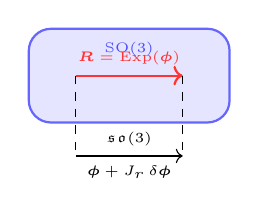
\begin{tikzpicture}[scale=0.85]
            % SO(3) manifold schematic
            \draw[thick, blue!60, fill=blue!10, rounded corners=8pt]
              (-1.5,-0.7) rectangle (1.5,0.7);
            \node[blue!70] at (0,0.4) {\tiny $\SOthree$};
            \draw[->, red!80, thick] (-0.8,0) -- (0.8,0)
              node[midway, above] {\tiny $\bm{R}=\Exp(\bm{\phi})$};
            \draw[->] (-0.8,-1.2) -- (0.8,-1.2)
              node[midway, below] {\tiny $\bm{\phi} + J_r\,\delta\bm{\phi}$};
            \draw[dashed] (-0.8,0) -- (-0.8,-1.2);
            \draw[dashed] (0.8,0) -- (0.8,-1.2);
            \node at (0,-0.95) {\tiny $\mathfrak{so}(3)$};
          \end{tikzpicture}
        \end{center}
        $J_r$: so(3)의 직선 이동을 SO(3) 곡면 위 이동으로 변환하는 ``왜곡 행렬''
      \end{block}
    \end{column}
    \begin{column}{0.48\textwidth}
      \begin{exampleblock}{직관적 이해}
        \begin{itemize}
          \item 평면에서: $\delta x$만큼 이동 = $\delta x$
          \item 구면에서: 법선 방향 이동은 없고, 접선 방향 이동만 --- 그 ``변환계수''가 $J_r$
          \item SO(3)에서: 각도가 클수록 $J_r$이 단위행렬에서 멀어짐 (공간이 더 많이 휨)
          \item $\phi \to 0$: 평탄해짐 $\Rightarrow$ $J_r \to I$
        \end{itemize}
      \end{exampleblock}
    \end{column}
  \end{columns}
\end{frame}


% ---------- SO3J-19
\begin{frame}[shrink=5]{SO(3) Jacobian과 쿼터니언(Quaternion) 비교}
  \begin{block}{쿼터니언 표현에서의 상황}
    단위 쿼터니언 $\bm{q} \in S^3$ ($\|\bm{q}\|=1$):
    \[
      \bm{q}(\bm{\phi}) = \begin{pmatrix}\cos\frac{\phi}{2} \\ \hat{\bm{\phi}}\sin\frac{\phi}{2}\end{pmatrix},
      \quad
      \bm{R}(\bm{q}) = (q_w^2 - \bm{q}_v^\top\bm{q}_v)I + 2\bm{q}_v\bm{q}_v^\top + 2q_w\skewx{\bm{q}_v}
    \]
  \end{block}
  \pause
  \begin{columns}[T]
    \begin{column}{0.50\textwidth}
      \begin{alertblock}{쿼터니언 Jacobian $\partial\bm{q}/\partial\bm{\phi}$}
        \[
          \frac{\partial\bm{q}}{\partial\bm{\phi}} = \frac{1}{2}
          \begin{pmatrix} -\bm{q}_v^\top \\ q_w I + \skewx{\bm{q}_v}\end{pmatrix}
          \in \R^{4\times 3}
        \]
        4차원 공간 $\subset \R^4$의 3차원 접선공간으로의 projection
      \end{alertblock}
    \end{column}
    \begin{column}{0.46\textwidth}
      \begin{block}{SO(3)와의 관계}
        $\bm{R}(\bm{q})$ Jacobian을 쿼터니언 경유로 계산:
        \[
          \frac{\partial\bm{R}}{\partial\bm{\phi}} = \frac{\partial\bm{R}}{\partial\bm{q}} \cdot \frac{\partial\bm{q}}{\partial\bm{\phi}}
        \]
        최종 결과는 SO(3) Jacobian과 동일\\
        (같은 기하학, 다른 표현)
      \end{block}
    \end{column}
  \end{columns}
  \pause
  \begin{exampleblock}{실용 결론}
    \begin{itemize}
      \item 쿼터니언 기반 코드에서도 결국 $J_r, J_l$이 등장함
      \item GTSAM의 \texttt{Rot3}, Ceres의 \texttt{QuaternionManifold} 모두 내부에서 동일한 Jacobian 계산
      \item 표현만 다를 뿐, \textbf{수학적 내용은 동일}
    \end{itemize}
  \end{exampleblock}
\end{frame}


% ---------- SO3J-20
\begin{frame}[shrink=25]{Solà (2018) 레퍼런스 --- \textit{A micro Lie theory}}
  \begin{block}{논문 정보}
    \begin{itemize}
      \item \textbf{제목}: ``A micro Lie theory for state estimation in robotics''
      \item \textbf{저자}: Joan Solà, Jeremie Deray, Dinesh Atchuthan
      \item \textbf{출처}: arXiv:1812.01537 (2018)  -- 누구나 무료 접근 가능
      \item \textbf{형식}: 58페이지 기술보고서 + 부록 (SLAM 커뮤니티 필독서)
    \end{itemize}
  \end{block}
  \pause
  \begin{columns}[T]
    \begin{column}{0.48\textwidth}
      \begin{block}{다루는 내용}
        \begin{itemize}
          \item SO(2), SO(3), SE(2), SE(3), Sim(3) 위의 Jacobian 통합 정리
          \item Right/Left Jacobian 폐쇄형
          \item BCH 근사, Adjoint
          \item Perturbation calculus 규칙 표 (Table 1)
          \item SLAM 응용 예시
        \end{itemize}
      \end{block}
    \end{column}
    \begin{column}{0.48\textwidth}
      \begin{alertblock}{핵심 Table (Solà 2018)}
        \footnotesize
        \begin{tabular}{ll}
          \hline
          공식 & 내용 \\
          \hline
          $\Exp(\phi+\delta) = \Exp(\phi)\Exp(J_r\delta)$ & 섭동 전파 \\
          $J_l = R\,J_r$ & Left-Right 관계 \\
          $J_r(-\phi) = J_l(\phi)$ & 부호 반전 \\
          $J_r^{-1} \approx I + \frac{1}{2}[\phi]_\times$ & 소각 역행렬 \\
          \hline
        \end{tabular}
      \end{alertblock}
    \end{column}
  \end{columns}
  \pause
  \vspace{0.3em}
  \begin{exampleblock}{권장 사항}
    \begin{center}
      이 자료 하나로 SO(3)/SE(3) Jacobian 문제는 대부분 해결된다.\\
      \textbf{robotics SLAM 연구자라면 반드시 읽어야 할 기준 문서.}
    \end{center}
  \end{exampleblock}
\end{frame}


% ---------- SO3J-21
\begin{frame}[shrink=5]{Solà (2018) 핵심 표: Lie 군 비교}
  \begin{block}{\small Lie 군들의 SO(3) Jacobian 구조 비교 (Solà 2018 기반)}
    \centering
    \footnotesize
    \begin{tabular}{l|ccc}
      \hline
      군 & 차원 & $J_r$ 크기 & 소각 근사 $J_r$ \\
      \hline
      $SO(2)$ & 1 & $1\times 1$ & $1$ (스칼라) \\
      $SO(3)$ & 3 & $3\times 3$ & $I - \frac{1}{2}[\phi]_\times$ \\
      $SE(2)$ & 3 & $3\times 3$ & $I - \frac{1}{2}[\xi]_\times$ \\
      $SE(3)$ & 6 & $6\times 6$ & $I - \frac{1}{2}[\xi]_\times^{(6)}$ \\
      $\mathrm{Sim}(3)$ & 7 & $7\times 7$ & 복잡한 구조 \\
      \hline
    \end{tabular}
  \end{block}
  \pause
  \begin{block}{\small SO(3) 주요 항등식 정리}
    \centering
    \footnotesize
    \renewcommand{\arraystretch}{1.4}
    \begin{tabular}{ll}
      \hline
      항등식 & 설명 \\
      \hline
      $\Exp(\phi)\Exp(\delta) = \Exp(\phi + J_l^{-1}\delta)$ (소각 $\delta$) & BCH 1차 \\
      $\Exp(\delta)\Exp(\phi) = \Exp(\phi + J_r^{-1}\delta)$ (소각 $\delta$) & BCH 1차 \\
      $R\,\Exp(\phi)\,R^\top = \Exp(R\phi)$ & Adjoint \\
      $J_l(\phi) = R\,J_r(\phi),\; R=\Exp(\phi)$ & L-R 관계 \\
      $J_r(\phi)^\top = J_r(-\phi) = J_l(\phi)^{-\top}$ & 전치 관계 \\
      \hline
    \end{tabular}
  \end{block}
\end{frame}


% ---------- SO3J-22
\begin{frame}[shrink=5]{SE(3) Jacobian 간략 소개}
  \begin{block}{SE(3): 위치+회전 함께}
    $\bm{T} = \begin{pmatrix}\bm{R} & \bm{t} \\ \bm{0} & 1\end{pmatrix} \in \SEthree$,\quad
    6D tangent: $\bm{\xi} = \begin{pmatrix}\bm{\rho} \\ \bm{\phi}\end{pmatrix} \in \R^6$ (translation + rotation)
    \[
      \Exp(\bm{\xi}) = \begin{pmatrix} \Exp(\bm{\phi}) & J_l(\bm{\phi})\bm{\rho} \\ \bm{0} & 1 \end{pmatrix}
    \]
  \end{block}
  \pause
  \begin{alertblock}{SE(3) Adjoint}
    \[
      \mathrm{Ad}_{\bm{T}} = \begin{pmatrix} \bm{R} & \skewx{\bm{t}}\bm{R} \\ \bm{0} & \bm{R} \end{pmatrix} \in \R^{6\times 6}
    \]
    6D twist(속도 스크류)를 한 좌표계에서 다른 좌표계로 변환할 때 사용
  \end{alertblock}
  \pause
  \begin{columns}[T]
    \begin{column}{0.50\textwidth}
      \begin{block}{SE(3) Right Jacobian}
        $6\times 6$ 행렬 (블록 구조):
        \[
          J_r^{SE(3)}(\bm{\xi}) = \begin{pmatrix} J_r(\bm{\phi}) & Q(\bm{\xi}) \\ \bm{0} & J_r(\bm{\phi}) \end{pmatrix}
        \]
        $Q(\bm{\xi})$: 위치-회전 coupling 항 (복잡한 형태)
      \end{block}
    \end{column}
    \begin{column}{0.46\textwidth}
      \begin{exampleblock}{9회차 LiDAR 섹션 preview}
        FAST-LIO, LOAM 등 LiDAR odometry에서:\\
        \medskip
        포인트 $\bm{p}$의 변환 $\bm{T}\bm{p}$ Jacobian:\\
        \[
          \frac{\partial(\bm{T}\bm{p})}{\partial\bm{\xi}}\bigg|_{\text{right}} = \begin{pmatrix} I & -\skewx{\bm{R}\bm{p}+\bm{t}} \end{pmatrix}
        \]
        SE(3) Jacobian이 ICP residual 최적화의 핵심
      \end{exampleblock}
    \end{column}
  \end{columns}
\end{frame}


% ---------- SO3J-22.5 — 미리보기 표지
\begin{frame}{\emph{미리보기}: 4회차 ESKF에서 $J_r$이 어떻게 쓰이는가}
  \begin{alertblock}{이 다음 3-4 슬라이드는 \textbf{4회차의 미리보기}}
    \begin{itemize}
      \item 4회차 ESKF는 ``명목 상태 + 오차 상태''를 분리해서 처리하는 구조
      \item 그 \textbf{오차 상태 전파식}에 $J_r$이 등장한다 — \emph{이걸 보여주기 위함}
      \item \alert{지금 단계에서 ESKF를 \emph{이해할 필요는 없다}}\\
            $J_r$이 ``실제로 어디서 쓰이는지'' 한 번 보고 넘어가는 게 목적
      \item 4회차에서 ESKF의 모든 줄을 처음부터 다시 유도한다
    \end{itemize}
  \end{alertblock}

  \pause
  \vspace{0.4em}
  \begin{exampleblock}{기억할 한 줄}
    \begin{center}
      $\bm{R} = \hatR\,\Exp(\dphivec)$ 의 시간 미분에서 \;\;$J_r$ \;\;이 자동으로 등장한다.
    \end{center}
  \end{exampleblock}

  \begin{center}\small\itshape\color{gray}
    학생: 다음 3-4 슬라이드는 \emph{빠르게 훑어}보고, 4회차에서 다시 만났을 때 ``아, 그때 본 것''이라고 알아채면 충분.
  \end{center}
\end{frame}

% ---------- SO3J-23
\begin{frame}[shrink=5]{(미리보기) ESKF error state dynamics와 $J_r$}
  \begin{block}{ESKF 오차 상태 전파 (회전 성분) \hfill \scriptsize\itshape 자세한 유도는 4회차}
    Nominal state: $\hatR_k$, Error state: $\dphivec_k$ (so(3) 벡터)
    \[
      \bm{R}_k = \hatR_k\,\Exp(\dphivec_k)
    \]
    한 스텝 propagation:
    \[
      \bm{R}_{k+1} = \bm{R}_k\,\Exp(\bm{\omega}\,\Delta t)
      \;\approx\; \hatR_{k+1}\,\Exp\!\left(A_\phi\,\dphivec_k + B_\phi\,\bm{n}_\omega\right)
    \]
  \end{block}
  \pause
  \begin{alertblock}{오차 전파 행렬 ($J_r$ 포함)}
    \[
      A_\phi = \Exp(-\hat{\bomega}\,\Delta t) \approx I - \skewx{\hat{\bomega}}\,\Delta t
    \]
    \[
      B_\phi = J_r(\hat{\bomega}\,\Delta t)\,\Delta t \approx I\,\Delta t \quad (\text{소각 근사})
    \]
    오차 공분산:
    \[
      P_{\phi,k+1} = A_\phi\,P_{\phi,k}\,A_\phi^\top + B_\phi\,Q_d\,B_\phi^\top
    \]
  \end{alertblock}
  \pause
  \begin{exampleblock}{실용 구현 수준}
    \begin{itemize}
      \item \textbf{기본 ESKF}: $J_r \approx I$ (소각 근사), 충분히 정확
      \item \textbf{정밀 구현}: Forster 2017처럼 $J_r(\hat{\bomega}\Delta t)$ 폐쇄형 계산
      \item IMU 100 Hz, $\Delta t = 0.01$ s, $\omega = 10$ rad/s: $\phi = 0.1$ rad ($\approx 5.7^\circ$)\\
            $\Rightarrow$ 소각 근사 충분히 유효
    \end{itemize}
  \end{exampleblock}
\end{frame}


% ---------- SO3J-24
\begin{frame}[shrink=5]{(미리보기) ESKF 업데이트: inject \& reset 단계의 Jacobian}
  \begin{block}{KF 업데이트 후 상태 주입 (State Injection)}
    추정된 error state $\delta\hat{\bm{\phi}}$를 nominal state에 합성:
    \[
      \hatR^+ = \hatR\,\Exp(\delta\hat{\bm{\phi}})
    \]
    이후 $\delta\hat{\bm{\phi}} \leftarrow \bm{0}$ (reset)
  \end{block}
  \pause
  \begin{alertblock}{Reset 후 공분산 보정: Reset Jacobian $G$}
    Reset 전 오차: $\dphivec_{\text{before}}$, Reset 후 오차: $\dphivec_{\text{after}}$
    \[
      \dphivec_{\text{after}} \approx \left(I - \frac{1}{2}\skewx{\delta\hat{\bm{\phi}}}\right)\dphivec_{\text{before}}
    \]
    Reset Jacobian:
    \[
      G = I - \frac{1}{2}\skewx{\delta\hat{\bm{\phi}}}
    \]
    공분산 업데이트: $P^+ = G\,(I - \bK\bH)\,P\,G^\top$
  \end{alertblock}
  \pause
  \begin{exampleblock}{출처 및 유도}
    \begin{itemize}
      \item Roumeliotis \& Burdick (2002), Mourikis \& Roumeliotis (2007)
      \item Joan Solà 박사 논문 (2010) ``Towards Visual Localization, Mapping and Moving Objects Tracking by a Mobile Robot''
      \item $G$는 사실상 $J_r^{-1}(\delta\hat{\bm{\phi}})$의 1차 근사
    \end{itemize}
  \end{exampleblock}
\end{frame}


% ---------- SO3J-25
\begin{frame}[shrink=20]{Right Jacobian의 고유값 분석}
  \begin{block}{$J_r(\bm{\phi})$의 행렬 구조}
    $\bm{\phi} = \phi\,\hat{\bm{n}}$ ($\hat{\bm{n}}$: 단위벡터)로 쓰면:
    \[
      J_r(\phi\hat{\bm{n}}) = \frac{\sin\phi}{\phi} P_\perp
      + \frac{1-\cos\phi}{\phi} \hat{\bm{n}}_\times
      + \hat{\bm{n}}\hat{\bm{n}}^\top
    \]
    여기서 $P_\perp = I - \hat{\bm{n}}\hat{\bm{n}}^\top$: $\hat{\bm{n}}$에 수직인 투영
  \end{block}
  \pause
  \begin{alertblock}{고유값}
    \begin{itemize}
      \item $\hat{\bm{n}}$ 방향: 고유값 $= 1$ (항상)
      \item $\hat{\bm{n}}$에 수직 방향: 복소 고유값 $\frac{\sin\phi}{\phi} \pm i\frac{1-\cos\phi}{\phi}$
      \item 크기: $\left|\frac{\sin\phi + i(1-\cos\phi)}{\phi}\right| = \frac{2\sin(\phi/2)}{\phi}$
    \end{itemize}
  \end{alertblock}
  \pause
  \begin{columns}[T]
    \begin{column}{0.50\textwidth}
      \begin{block}{$\det(J_r(\phi))$}
        \[
          \det(J_r) = \frac{2(1-\cos\phi)}{\phi^2} \cdot 1 = \left(\frac{2\sin(\phi/2)}{\phi}\right)^2
        \]
        $\phi \to 0$: $\det \to 1$\\
        $\phi = \pi$: $\det \to 0$ (singular!)
      \end{block}
    \end{column}
    \begin{column}{0.46\textwidth}
      \begin{exampleblock}{Singularity 주의}
        $\phi = \pi$ (180도 회전): $J_r$ 특이!\\
        $\Rightarrow$ $J_r^{-1}$ 존재하지 않음\\
        \medskip
        실용적으로: $\|\bm{\phi}\| < \pi$에서만 사용\\
        Gimbal lock과 유사한 문제
      \end{exampleblock}
    \end{column}
  \end{columns}
\end{frame}


% ---------- SO3J-26
\begin{frame}[shrink=5]{$J_r$와 평행이동 Jacobian의 결합: SE(3) 응용}
  \begin{block}{SE(3) Exp의 평행이동 성분}
    $\bm{\xi} = (\bm{\rho}, \bm{\phi})^\top$에 대해 $\bm{T} = \Exp(\bm{\xi})$이면:
    \[
      \bm{t} = J_l(\bm{\phi})\,\bm{\rho}
    \]
    평행이동 $\bm{t}$은 $\bm{\rho}$에 Left Jacobian을 곱한 것
  \end{block}
  \pause
  \begin{columns}[T]
    \begin{column}{0.50\textwidth}
      \begin{alertblock}{실용 의미}
        $\bm{\phi} \to \bm{0}$ (소각 회전): $J_l \to I$\\
        $\Rightarrow$ $\bm{t} \approx \bm{\rho}$ (직관적)\\
        \medskip
        큰 회전: $J_l$이 $\bm{\rho}$를 휘게 만들어\\
        나선형 운동(screw motion)을 표현
      \end{alertblock}
    \end{column}
    \begin{column}{0.46\textwidth}
      \begin{exampleblock}{FAST-LIO2에서 사용}
        LiDAR scan-to-map 오차 Jacobian:\\
        \[
          \bm{J} = \begin{pmatrix} \bm{n}^\top J_l^\top & \bm{n}^\top\skewx{\bm{T}\bm{p}} \end{pmatrix}
        \]
        포인트-평면 거리의 6D pose Jacobian\\
        ($\bm{n}$: 평면 법선벡터)
      \end{exampleblock}
    \end{column}
  \end{columns}
  \pause
  \vspace{0.3em}
  \begin{block}{요약}
    \begin{center}
      SE(3) Jacobian = SO(3)의 $J_r/J_l$ + 위치-회전 coupling 항 $Q$\\
      로봇 SLAM의 pose optimization 전체가 이 구조 위에 구축됨
    \end{center}
  \end{block}
\end{frame}


% ---------- SO3J-27
\begin{frame}[shrink=25]{정리: SO(3) Jacobian 공식 모음}
  \begin{alertblock}{Right Jacobian $J_r(\bm{\phi})$}
    \small
    \[
      J_r = I - \frac{1-\cos\phi}{\phi^2}[\bm{\phi}]_\times + \frac{\phi-\sin\phi}{\phi^3}[\bm{\phi}]_\times^2
      \;\xrightarrow{\phi\to 0}\; I - \tfrac{1}{2}[\bm{\phi}]_\times
    \]
  \end{alertblock}
  \begin{alertblock}{Right Jacobian Inverse $J_r^{-1}(\bm{\phi})$}
    \small
    \[
      J_r^{-1} = \frac{\phi}{2}\cot\frac{\phi}{2}I + \left(1-\frac{\phi}{2}\cot\frac{\phi}{2}\right)\hat{\bm{\phi}}\hat{\bm{\phi}}^\top + \frac{\phi}{2}[\hat{\bm{\phi}}]_\times
      \;\xrightarrow{\phi\to 0}\; I + \tfrac{1}{2}[\bm{\phi}]_\times
    \]
  \end{alertblock}
  \begin{block}{\small 관계식 모음}
    \footnotesize
    \renewcommand{\arraystretch}{1.3}
    \begin{tabular}{ll}
      $J_l(\bm{\phi}) = J_r(-\bm{\phi})$ & $J_l = R\,J_r,\; R=\Exp(\bm{\phi})$ \\
      $\Exp(\bm{\phi}+\delta) = \Exp(\bm{\phi})\Exp(J_r\delta)$ & $\Exp(\bm{\phi}+\delta) = \Exp(J_l\delta)\Exp(\bm{\phi})$ \\
      $\Log(\Exp(\bm{a})\Exp(\bm{b})) \approx \bm{a} + J_l^{-1}(\bm{a})\bm{b}$ & $R\Exp(\bm{\phi})R^\top = \Exp(R\bm{\phi})$ \\
      $\Sigma_{\SOthree} = J_r Q J_r^\top$ & $G_{\text{reset}} = I - \tfrac{1}{2}[\delta\hat{\bm{\phi}}]_\times$ \\
    \end{tabular}
  \end{block}
\end{frame}


% ---------- SO3J-28
\begin{frame}{연습 문제 (1): Right Jacobian 계산}
  \begin{block}{문제 1}
    $\bm{\phi} = (0, 0, \pi/6)^\top$ (z축 30도 회전)일 때:
    \begin{enumerate}
      \item $J_r(\bm{\phi})$를 폐쇄형 공식으로 계산하시오.
      \item 소각 근사 $J_r \approx I - \frac{1}{2}[\bm{\phi}]_\times$와 비교하시오.
      \item Frobenius norm 오차 $\|J_r^{\text{exact}} - J_r^{\text{approx}}\|_F$를 구하시오.
    \end{enumerate}
  \end{block}
  \pause
  \begin{exampleblock}{힌트}
    $\phi = \pi/6$, $\skewx{\bm{\phi}} = \phi\begin{pmatrix}0&-1&0\\1&0&0\\0&0&0\end{pmatrix}$:
    \begin{align*}
      J_r &= I - \frac{1-\cos(\pi/6)}{(\pi/6)^2}[\bm{\phi}]_\times + \frac{\pi/6-\sin(\pi/6)}{(\pi/6)^3}[\bm{\phi}]_\times^2 \\
      &\approx \begin{pmatrix}0.9589 & -0.2588 & 0 \\ 0.2588 & 0.9589 & 0 \\ 0 & 0 & 1\end{pmatrix}
    \end{align*}
    (수치 계산 검증: Python/MATLAB 권장)
  \end{exampleblock}
\end{frame}


% ---------- SO3J-29
\begin{frame}{연습 문제 (2): 섭동 전파}
  \begin{block}{문제 2}
    $\bm{R}_0 = \Exp(\bm{\phi}_0)$, $\bm{\phi}_0 = (\pi/4, 0, 0)^\top$이고\\
    $\delta\bm{\phi} = (0.01, 0.01, 0.01)^\top$이라 할 때:
    \begin{enumerate}
      \item $\Exp(\bm{\phi}_0 + \delta\bm{\phi})$를 직접 계산하시오.
      \item $\bm{R}_0\,\Exp(J_r(\bm{\phi}_0)\,\delta\bm{\phi})$를 계산하시오.
      \item 두 결과의 차이를 $\|\cdot\|_F$로 측정하고, 이것이 $O(\|\delta\bm{\phi}\|^2)$인지 확인하시오.
    \end{enumerate}
  \end{block}
  \pause
  \begin{block}{문제 3: BCH 검증}
    $\bm{a} = (\pi/3, 0, 0)^\top$, $\bm{b} = (0, 0.05, 0)^\top$일 때:
    \begin{enumerate}
      \item $\Log(\Exp(\bm{a})\Exp(\bm{b}))$를 수치적으로 계산하시오.
      \item BCH 1차 근사 $\bm{a} + J_l^{-1}(\bm{a})\bm{b}$와 비교하시오.
      \item 0차 근사 $\bm{a} + \bm{b}$와도 비교하시오.
    \end{enumerate}
    BCH 1차 근사가 왜 더 나은지 설명하시오.
  \end{block}
\end{frame}


% ---------- SO3J-30
\begin{frame}[shrink=5]{연습 문제 (3): \emph{미리보기} ESKF 적용 (선택)}
  \begin{block}{문제 4: 공분산 변환}
    초기 회전 오차 공분산 $P_\phi = \sigma^2 I$, $\sigma = 0.1$ rad이고\\
    $\hat{\bm{\phi}} = (0.3, 0.2, 0.1)^\top$ rad ($\|\hat{\bm{\phi}}\| \approx 0.374$ rad)에서:
    \begin{enumerate}
      \item $J_r(\hat{\bm{\phi}})$를 계산하시오.
      \item SO(3) 공분산 $\Sigma_{\SOthree} = J_r P_\phi J_r^\top$를 계산하시오.
      \item $J_r \approx I$ 근사와의 차이를 비교하시오.
    \end{enumerate}
  \end{block}
  \pause
  \begin{block}{문제 5: ESKF Reset Jacobian}
    업데이트 후 $\delta\hat{\bm{\phi}} = (0.05, -0.03, 0.02)^\top$이 추정되었을 때:
    \begin{enumerate}
      \item Reset Jacobian $G = I - \frac{1}{2}[\delta\hat{\bm{\phi}}]_\times$를 계산하시오.
      \item 이것이 $J_r^{-1}(\delta\hat{\bm{\phi}})$의 1차 근사임을 보이시오.
      \item 업데이트 후 공분산 $P^+ = G(I-KH)PG^\top$에서\\
            $G$를 생략했을 때의 오차를 quantify 하시오.
    \end{enumerate}
  \end{block}
\end{frame}


% ---------- SO3J-31
\begin{frame}[shrink=5]{심화: Jacobian of composition $\bm{R}_1\bm{R}_2$}
  \begin{block}{회전 합성의 Jacobian (right perturbation)}
    $f(\bm{R}_1, \bm{R}_2) = \bm{R}_1\bm{R}_2$에서 각각에 대한 Jacobian:
  \end{block}
  \begin{columns}[T]
    \begin{column}{0.48\textwidth}
      \begin{alertblock}{$\bm{R}_1$ w.r.t. right perturbation}
        \[
          \frac{\partial(\bm{R}_1\bm{R}_2)}{\partial\delta\bm{\phi}_1}\bigg|_{\text{right}}
          = I_{3\times 3}
        \]
        (right perturbation으로 $\bm{R}_1$ 섭동 시 합성 회전도 같은 방향)
      \end{alertblock}
    \end{column}
    \begin{column}{0.48\textwidth}
      \begin{alertblock}{$\bm{R}_2$ w.r.t. right perturbation}
        \[
          \frac{\partial(\bm{R}_1\bm{R}_2)}{\partial\delta\bm{\phi}_2}\bigg|_{\text{right}}
          = \bm{R}_1^\top \cdot I \cdot \bm{R}_1 = I
        \]
        (Adjoint에 의해 좌표계 변환)\\
        \medskip
        정확히는: $\text{Ad}_{\bm{R}_1^\top} = \bm{R}_1^\top$
      \end{alertblock}
    \end{column}
  \end{columns}
  \pause
  \vspace{0.4em}
  \begin{block}{역회전 $\bm{R}^{-1} = \bm{R}^\top$의 Jacobian}
    \[
      \frac{\partial(\bm{R}^\top)}{\partial\delta\bm{\phi}}\bigg|_{\text{right}} = -I_{3\times 3}
    \]
    (직관: 회전 방향을 뒤집으면 Jacobian 부호도 반전)
  \end{block}
  \pause
  \begin{exampleblock}{Factor graph에서의 활용}
    IMU factor의 rotation residual: $\bm{r} = \Log(\bm{R}_i^\top\bm{R}_j\,\Delta R_{ij}^\top)$\\
    \[
      \frac{\partial\bm{r}}{\partial\delta\bm{\phi}_i}\bigg|_{\text{right}} = -J_l^{-1}(\bm{r}),
      \qquad
      \frac{\partial\bm{r}}{\partial\delta\bm{\phi}_j}\bigg|_{\text{right}} = J_l^{-1}(\bm{r})\,\bm{R}_i^\top\bm{R}_j\,\Delta R_{ij}^\top\cdot(-1)\cdot\ldots
    \]
  \end{exampleblock}
\end{frame}


% ---------- SO3J-32
\begin{frame}[shrink=5]{SO(3) Jacobian과 로봇 제어: 연결}
  \begin{block}{운동학적 Jacobian (Geometric Jacobian) 복습}
    로봇 말단 각속도: $\bomega = J_\omega(\bm{q})\,\dot{\bm{q}}$\\
    이것과 SO(3) Jacobian은 \textbf{다른 개념}이지만 연결됨
  \end{block}
  \pause
  \begin{columns}[T]
    \begin{column}{0.50\textwidth}
      \begin{block}{Lie 대수적 해석}
        SO(3)에서 body angular velocity $\bomega$:
        \[
          \bm{R}^\top\dot{\bm{R}} = \skewx{\bomega^b} \in \mathfrak{so}(3)
        \]
        $\bomega^b = J_r^{-1}(\bm{\phi})\,\dot{\bm{\phi}}$ (right body velocity)\\
        \medskip
        $\Rightarrow$ $J_r^{-1}$가 관절 속도 $\dot{\bm{\phi}}$를\\
        body angular velocity $\bomega^b$로 변환
      \end{block}
    \end{column}
    \begin{column}{0.46\textwidth}
      \begin{exampleblock}{응용: 오일러각 Jacobian}
        오일러각 $(\psi, \theta, \phi)$에서도 유사한 구조:
        \[
          \bomega = E(\psi,\theta,\phi)\,\dot{\bm{\Theta}}
        \]
        $E$: 오일러각 ``Jacobian'' (비특이 조건: $\theta \neq \pm90^\circ$)\\
        SO(3) 전역 $J_r$과 유사한 역할이지만 좌표 의존적
      \end{exampleblock}
    \end{column}
  \end{columns}
  \pause
  \vspace{0.3em}
  \begin{alertblock}{핵심 차이}
    \begin{center}
      SO(3) $J_r$: 좌표 독립적 (차표계 선택 불필요)\\
      오일러각 $E$: 특정 좌표계 의존적, singularity 존재\\
      $\Rightarrow$ ESKF에서 $J_r$ 기반 접근이 더 강건
    \end{center}
  \end{alertblock}
\end{frame}


% ---------- SO3J-33
\begin{frame}[shrink=5]{SO(3) Jacobian: 학습 로드맵}
  \begin{block}{이 파트에서 배운 핵심 개념 흐름}
    \footnotesize
    \begin{enumerate}
      \item \textbf{동기}: SO(3)는 벡터공간이 아니므로 미분에 접선공간(tangent space) 필요
      \item \textbf{Right perturbation}: $f(\bm{R}\Exp(\epsilon))$의 극한 $\rightarrow$ right Jacobian
      \item \textbf{$J_r$ 정의}: 적분 $\rightarrow$ 폐쇄형, $\phi\to 0$이면 $I$
      \item \textbf{$J_l = J_r(-\phi)$}: Adjoint로 연결
      \item \textbf{$J_r^{-1}$ 폐쇄형}: 소각 근사 $I + \tfrac{1}{2}[\phi]_\times$
      \item \textbf{소각 근사}: ESKF 표준, $<10^\circ$에서 유효
      \item \textbf{BCH 1차}: $\Log(\Exp a\Exp b) \approx a + J_l^{-1}b$
      \item \textbf{섭동 전파}: $\Exp(\phi+\delta) = \Exp(\phi)\Exp(J_r\delta)$
      \item \textbf{공분산 변환}: $\Sigma_{\SOthree} = J_r Q J_r^\top$
      \item \textbf{ESKF 적용}: preintegration, inject/reset Jacobian
    \end{enumerate}
  \end{block}
  \pause
  \begin{columns}[T]
    \begin{column}{0.48\textwidth}
      \begin{block}{다음 강의에서의 사용처}
        \begin{itemize}
          \item \textbf{4회차}: ESKF 전체 유도에서 $J_r$ 등장
          \item \textbf{5회차}: IMU preintegration 공분산에서 $J_r^{(k)}$
          \item \textbf{7/8회차}: VIO factor graph residual Jacobian
          \item \textbf{9회차}: LiDAR SE(3) Jacobian
        \end{itemize}
      \end{block}
    \end{column}
    \begin{column}{0.48\textwidth}
      \begin{exampleblock}{참고문헌}
        \begin{itemize}
          \item Solà \textit{et al.} arXiv:1812.01537
          \item Forster \textit{et al.} TRO 2017
          \item Chirikjian (2012) \textit{Stochastic Models...}
          \item Barfoot (2017) \textit{State Estimation for Robotics}
        \end{itemize}
      \end{exampleblock}
    \end{column}
  \end{columns}
\end{frame}


% ---------- SO3J-34
\begin{frame}[shrink=5]{회차 요약: SO(3) Jacobians}
  \begin{alertblock}{\large 5대 핵심 공식}
    \begin{enumerate}
      \item \textbf{$J_r(\bm{\phi})$ 정의 (폐쇄형)}:
            \[
              J_r(\bm{\phi}) = I - \frac{1-\cos\phi}{\phi^2}[\bm{\phi}]_\times + \frac{\phi-\sin\phi}{\phi^3}[\bm{\phi}]_\times^2
            \]
      \item \textbf{Left-Right 관계}:
            \[
              J_l(\bm{\phi}) = J_r(-\bm{\phi}) = \Exp(\bm{\phi})\,J_r(\bm{\phi})
            \]
      \item \textbf{소각 근사}:
            \[
              J_r(\bm{\phi}) \approx I - \tfrac{1}{2}[\bm{\phi}]_\times, \quad
              J_r^{-1}(\bm{\phi}) \approx I + \tfrac{1}{2}[\bm{\phi}]_\times
            \]
      \item \textbf{섭동 전파} (ESKF/preintegration 핵심):
            \[
              \Exp(\bm{\phi}+\delta\bm{\phi}) = \Exp(\bm{\phi})\,\Exp\!\left(J_r(\bm{\phi})\,\delta\bm{\phi}\right)
            \]
      \item \textbf{공분산 변환}:
            \[
              \Sigma_{\SOthree} = J_r(\bm{\phi})\,\Sigma_{\mathfrak{so}(3)}\,J_r(\bm{\phi})^\top
            \]
    \end{enumerate}
  \end{alertblock}
\end{frame}


% ---------- SO3J-35
\begin{frame}{다음 회차 예고: 3회차 선형 KF, 4회차 ESKF}
  \begin{block}{2회차 전체 정리}
    \begin{itemize}
      \item SO(3) 기초: 군 구조, Exp/Log map, Rodrigues 공식
      \item Right perturbation: ESKF의 기본 관례
      \item \textbf{SO(3) Jacobians}: $J_r, J_l$, BCH, 섭동 전파, 공분산 변환
    \end{itemize}
  \end{block}
  \pause
  \begin{alertblock}{4회차(ESKF)에서 다시 만날 핵심 도구 — 미리 보기}
    \begin{columns}[T]
      \begin{column}{0.50\textwidth}
        \begin{itemize}
          \item Right perturbation: $\bm{R} = \hatR\,\Exp(\dphivec)$
          \item 선형화: $\Exp(\dphivec) \approx I + \skewx{\dphivec}$
          \item Error dynamics: $J_r^{-1}$ 포함한 $F$ 행렬
          \item Noise 전파: $J_r\,Q_d\,J_r^\top$
        \end{itemize}
      \end{column}
      \begin{column}{0.46\textwidth}
        \begin{itemize}
          \item Update: $\hatR \leftarrow \hatR\,\Exp(\delta\hat{\bm{\phi}})$
          \item Reset Jacobian: $G = I - \tfrac{1}{2}[\delta\hat{\bm{\phi}}]_\times$
          \item Full ESKF: 15D error state\\
                $\dxvec = (\dphivec, \dpvec, \dvvec, \dbgvec, \dbavec)^\top$
        \end{itemize}
      \end{column}
    \end{columns}
  \end{alertblock}
  \pause
  \begin{center}
    \large\textbf{먼저 3회차 (선형 KF) → 다음 4회차에서 ESKF 전체 유도}
  \end{center}
  \begin{center}
    \small 참고: Joan Solà (2017) ``Quaternion kinematics for the error-state Kalman filter''\\
    arXiv:1711.02508 --- ESKF 최고의 입문 자료
  \end{center}
\end{frame}

% ========== L2 확장 끝 ==========

\section{3회차: 선형 Kalman Filter}
% ---------- 1


% ---------- 2
\begin{frame}{지난 시간 한 줄}
  \begin{center}
    \large
    SO(3)는 3D 회전의 매니폴드. \\
    tangent space $\sothree \cong \mathbb{R}^3$ $\rightarrow$ error state $\dphivec$는 제약 없는 벡터.
  \end{center}
  \vspace{0.5em}
  오늘의 목표:
  \begin{itemize}
    \item \emph{선형} 시스템에서 KF의 다섯 줄을 \textbf{손으로} 유도
    \item 각 줄의 \emph{왜}를 한 마디로 말하기
    \item 1D 위치+속도 KF Python 30줄로 belief가 춤추는 모습 관찰
  \end{itemize}
\end{frame}

% ---------- 3
\begin{frame}{선형 시스템의 정의}
  \[
    \bx_{k} = \bF \bx_{k-1} + \bB \bu_k + \bw_k, \quad \bw_k \sim \Norm{\bzero}{\bQ}
  \]
  \[
    \bz_{k} = \bH \bx_{k} + \bv_k, \quad \bv_k \sim \Norm{\bzero}{\bR}
  \]
  \begin{itemize}
    \item $\bF$: state transition matrix
    \item $\bB$: 입력 게인 (선택 — 없으면 0)
    \item $\bH$: 측정 행렬
    \item $\bw, \bv$: 가우시안 잡음, 서로 독립
  \end{itemize}
  \pause
  \vspace{0.3em}
  \begin{block}{필수 가정 4개}
    선형 process, 선형 측정, 가우시안 잡음, 잡음 독립.
  \end{block}
\end{frame}

% ---------- 4
\begin{frame}{왜 \emph{이 가정}들이 KF를 살리는가}
  \begin{itemize}
    \item 선형 변환은 가우시안을 \emph{또 가우시안}으로 보낸다 (1회차 보조 정리)
    \item 가우시안의 곱도 가우시안 (1회차 보조 정리)
    \item 그래서 prior가 가우시안이면 \emph{영원히} 가우시안
    \item belief가 \textbf{(평균, 공분산)}만으로 완전 기술됨 → 컴퓨터로 풀 수 있음
  \end{itemize}
  \pause
  \vspace{0.5em}
  \begin{block}{핵심}
    KF의 5줄은 모두 \emph{이 두 보조 정리의 적용}에 불과하다.
  \end{block}
\end{frame}

% ---------- 5
\begin{frame}{표기 정리 (이번 회차 내내)}
  \begin{itemize}
    \item $\hat\bx_{k|k-1}$: $k-1$까지의 측정으로 $k$를 \emph{예측}한 평균 (prior)
    \item $\bP_{k|k-1}$: 그 분포의 공분산
    \item $\hat\bx_{k|k}$: $k$의 측정까지 \emph{흡수}한 평균 (posterior)
    \item $\bP_{k|k}$: 그 공분산
  \end{itemize}
  \pause
  \vspace{0.3em}
  Bayes filter 그림으로 다시:
  \begin{center}
  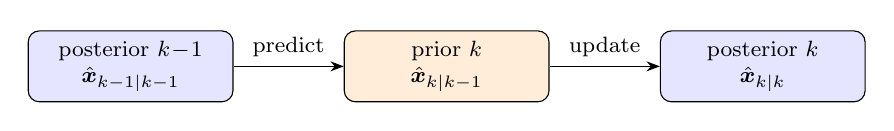
\begin{tikzpicture}[font=\footnotesize, node distance=1.0cm,
    blk/.style={draw, rounded corners, minimum height=0.9cm, minimum width=2.6cm, align=center}]
    \node[blk, fill=blue!10]   (a) {posterior $k\!-\!1$\\$\hat\bx_{k-1|k-1}$};
    \node[blk, fill=orange!15, right=1.4cm of a] (b) {prior $k$\\$\hat\bx_{k|k-1}$};
    \node[blk, fill=blue!10,   right=1.4cm of b] (c) {posterior $k$\\$\hat\bx_{k|k}$};
    \draw[-Stealth] (a) -- node[above]{predict} (b);
    \draw[-Stealth] (b) -- node[above]{update}  (c);
  \end{tikzpicture}
  \end{center}
\end{frame}

% ---------- 6
\begin{frame}{Predict 유도 (1) — 평균}
  $\bx_{k} = \bF \bx_{k-1} + \bB \bu_k + \bw_k$ 의 양변에 기댓값:
  \[
    \E[\bx_k \mid \bz_{1:k-1}] \;=\; \bF\, \E[\bx_{k-1} \mid \bz_{1:k-1}] + \bB \bu_k
  \]
  \pause
  \vspace{0.3em}
  \begin{block}{Predict 평균 식}
    \[
      \boxed{\;\hat\bx_{k|k-1} \;=\; \bF\, \hat\bx_{k-1|k-1} + \bB \bu_k\;}
    \]
  \end{block}
  잡음 $\bw_k$의 기댓값이 0이라 사라짐. 평균은 단순히 \emph{선형으로 옮긴} 것.
\end{frame}

% ---------- 7
\begin{frame}{Predict 유도 (2) — 공분산}
  편차 정의: $\bm{e}_k = \bx_k - \hat\bx_{k|k-1}$\\
  $\bm{e}_k = \bF (\bx_{k-1} - \hat\bx_{k-1|k-1}) + \bw_k = \bF \bm{e}_{k-1} + \bw_k$
  \pause
  \vspace{0.4em}
  공분산은 $\E[\bm{e}_k \bm{e}_k^\top]$:
  \[
    \bP_{k|k-1} = \bF\, \E[\bm{e}_{k-1}\bm{e}_{k-1}^\top]\, \bF^\top + \E[\bw_k \bw_k^\top]
  \]
  ($\bm{e}_{k-1}$과 $\bw_k$가 독립이라 교차항 사라짐)
  \pause
  \vspace{0.3em}
  \begin{block}{Predict 공분산 식}
    \[
      \boxed{\;\bP_{k|k-1} \;=\; \bF\, \bP_{k-1|k-1}\, \bF^\top + \bQ\;}
    \]
  \end{block}
\end{frame}

% ---------- 8
\begin{frame}{Predict의 의미 한 마디}
  \begin{itemize}
    \item \textbf{평균}은 dynamics를 따라 \emph{흘러간다}
    \item \textbf{공분산}은 dynamics에 의해 \emph{회전/늘어나고} ($\bF \bP \bF^\top$), process noise만큼 \emph{커진다} ($+\bQ$)
    \item 직관: "예측만 하면 belief는 점점 \emph{퍼진다}"
  \end{itemize}
  \pause
  \vspace{0.4em}
  \begin{center}
  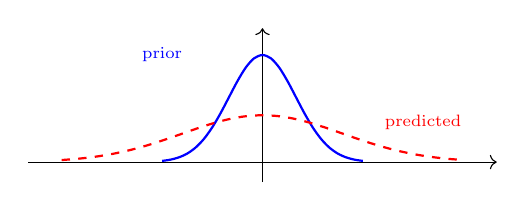
\begin{tikzpicture}[scale=0.85, transform shape]
    \draw[->] (-3.5,0) -- (3.5,0); \draw[->] (0,-0.3) -- (0,2);
    \draw[domain=-1.5:1.5, smooth, thick, blue]   plot (\x, {1.6*exp(-\x*\x/(2*0.5*0.5))});
    \draw[domain=-3:3, smooth, thick, red, dashed] plot (\x, {0.7*exp(-\x*\x/(2*1.2*1.2))});
    \node[blue] at (-1.5,1.6) {\scriptsize prior};
    \node[red]  at ( 2.4,0.6) {\scriptsize predicted};
  \end{tikzpicture}
  \end{center}
\end{frame}

% ---------- 9
\begin{frame}{Update 유도의 두 갈래}
  같은 답에 도달하는 두 길:
  \begin{enumerate}
    \item \textbf{가우시안 곱셈} 길 (1회차의 1D 결과를 일반화)
    \item \textbf{최적 추정량} 길 (innovation 잔차의 분산을 최소화)
  \end{enumerate}
  \pause
  \vspace{0.4em}
  여기선 \emph{직관적}인 (2)번 길로 간다 — Kalman의 1960년 논문 길이기도 함.
\end{frame}

% ---------- 10
\begin{frame}{Update 유도 (1) — 추정 형태 가정}
  posterior 평균을 \emph{선형 보정} 형태로 가정:
  \[
    \hat\bx_{k|k} \;=\; \hat\bx_{k|k-1} + \bK\,\bigl(\bz_k - \bH \hat\bx_{k|k-1}\bigr)
  \]
  \begin{itemize}
    \item $\bK$: 아직 모르는 게인 행렬
    \item $\bz_k - \bH \hat\bx_{k|k-1}$: \textbf{innovation} (혁신, 측정과 예측의 차이)
  \end{itemize}
  \pause
  \vspace{0.3em}
  \begin{block}{질문}
    posterior의 \emph{공분산}을 가장 작게 만드는 $\bK$는?
  \end{block}
\end{frame}

% ---------- 11
\begin{frame}{Update 유도 (2) — posterior 공분산}
  \footnotesize
  $\bm{e}_k = \bx_k - \hat\bx_{k|k}$, $\tilde{\bm{e}}_k = \bx_k - \hat\bx_{k|k-1}$ (predict 잔차)\\
  innovation: $\bz_k - \bH\hat\bx_{k|k-1} = \bH\tilde{\bm{e}}_k + \bv_k$
  \pause
  \vspace{0.2em}
  대입:
  \[
    \bm{e}_k = \tilde{\bm{e}}_k - \bK(\bH\tilde{\bm{e}}_k + \bv_k) = (\bI - \bK\bH)\tilde{\bm{e}}_k - \bK\bv_k
  \]
  \pause
  \vspace{0.2em}
  공분산:
  \[
    \bP_{k|k} = (\bI-\bK\bH)\,\bP_{k|k-1}\,(\bI-\bK\bH)^\top + \bK \bR \bK^\top
  \]
  이게 \textbf{Joseph form}. 다음 슬라이드에서 단순화.
\end{frame}

% ---------- 12
\begin{frame}{Update 유도 (3) — 최적 게인}
  \footnotesize
  $\bP_{k|k}$의 \emph{trace}를 최소화하는 $\bK$를 찾자 (총 분산 최소).
  \[
    \frac{\partial}{\partial \bK} \mathrm{tr}\,\bP_{k|k} = 0
  \]
  \pause
  편미분 (행렬 미분 공식 활용) 후 정리:
  \[
    -2(\bI - \bK\bH)\,\bP_{k|k-1}\,\bH^\top + 2\bK\bR = \bzero
  \]
  \pause
  $\bK$에 대해 풀면:
  \[
    \boxed{\;\bK \;=\; \bP_{k|k-1}\,\bH^\top \bigl(\bH\,\bP_{k|k-1}\,\bH^\top + \bR\bigr)^{-1}\;}
  \]
  \vspace{0.3em}
  $\bS = \bH\bP_{k|k-1}\bH^\top + \bR$ — \textbf{innovation 공분산}.
\end{frame}

% ---------- 13
\begin{frame}{Kalman gain의 의미}
  \[
    \bK = \bP \bH^\top \bS^{-1}
  \]
  \begin{itemize}
    \item $\bP \bH^\top$: state ↔ 측정의 \emph{cross-covariance}
    \item $\bS^{-1}$: 측정 공간에서의 \emph{역분산} (= 정밀도)
    \item 둘의 곱 = "측정 정보를 state로 \emph{끌어오는} 변환"
  \end{itemize}
  \pause
  \vspace{0.4em}
  \begin{block}{한계 사례}
    \begin{itemize}
      \item $\bR \to 0$: 완벽한 측정 → $\bK \to \bH^\dagger$ (측정값을 그대로 신뢰)
      \item $\bR \to \infty$: 무의미한 측정 → $\bK \to 0$ (측정 무시, predict만 사용)
    \end{itemize}
  \end{block}
\end{frame}

% ---------- 14
\begin{frame}{Update 유도 (4) — posterior 공분산: Joseph form이 표준}
  최적 $\bK$를 대입하면 두 가지 형태:
  \[
    \text{짧은 형} \quad \bP_{k|k} = (\bI - \bK\bH)\,\bP_{k|k-1}
    \quad \leftarrow \text{수학적으로는 같지만 수치 불안정}
  \]
  \pause
  \[
    \boxed{\;\bP_{k|k} = (\bI-\bK\bH)\,\bP_{k|k-1}\,(\bI-\bK\bH)^\top + \bK\bR\bK^\top\;}
    \quad \leftarrow \textbf{Joseph form}
  \]
  \pause
  \vspace{0.3em}
  \begin{block}{Joseph form을 \emph{항상} 써야 하는 이유}
    짧은 형은 최적 $\bK$일 때만 양정치성을 보장.\\
    부동소수점 오차, 부정확한 $\bK$ 상황에서도 Joseph form은 \emph{구조적으로} 양정치.\\
    $(\bA\bP\bA^\top + \bK\bR\bK^\top)$ — 두 항 모두 양반정치의 합 $\Rightarrow$ 항상 양반정치.\\
    \textbf{실무 규칙: 항상 Joseph form. 짧은 형은 쓰지 않는다.}
  \end{block}
\end{frame}

% ---------- 15
\begin{frame}{이걸로 KF 완성 — Joseph form 포함 표준 버전}
  \footnotesize
  \textbf{Predict}
  \[
    \hat\bx_{k|k-1} = \bF \hat\bx_{k-1|k-1} + \bB \bu_k
  \]
  \[
    \bP_{k|k-1} = \bF \bP_{k-1|k-1} \bF^\top + \bQ
  \]
  \textbf{Update}
  \[
    \bK = \bP_{k|k-1} \bH^\top (\bH \bP_{k|k-1} \bH^\top + \bR)^{-1}
  \]
  \[
    \hat\bx_{k|k} = \hat\bx_{k|k-1} + \bK\,(\bz_k - \bH \hat\bx_{k|k-1})
  \]
  \[
    \bP_{k|k} = \underbrace{(\bI - \bK\bH)\,\bP_{k|k-1}\,(\bI-\bK\bH)^\top
                            + \bK\bR\bK^\top}_{\textbf{Joseph form — 항상 이것}}
  \]
  \pause
  \vspace{0.2em}
  외울 필요 없다. \emph{유도할 줄 알면} 평생 본인 것. Joseph form만 기억하면 됨.
\end{frame}

% ---------- 16
\begin{frame}{각 줄을 한 마디로}
  \footnotesize
  \begin{itemize}
    \item \textbf{$\hat\bx_{k|k-1} = \bF \hat\bx_{k-1|k-1}$}: 평균을 dynamics로 옮긴다
    \item \textbf{$\bP_{k|k-1} = \bF\bP\bF^\top + \bQ$}: 공분산을 늘리고, process noise만큼 더 부푼다
    \item \textbf{$\bK = \bP\bH^\top \bS^{-1}$}: 측정 정밀도와 cross-covariance의 곱 = 측정에서 state로의 게인
    \item \textbf{$\hat\bx_{k|k} = \hat\bx_{k|k-1} + \bK\,\bm{r}$}: 잔차에 게인을 곱해 평균 보정
    \item \textbf{$\bP_{k|k} = (\bI-\bK\bH)\bP$}: 측정만큼 공분산이 \emph{줄어든다}
  \end{itemize}
\end{frame}

% ---------- 17
\begin{frame}{1D KF는 1회차 보조 정리와 \emph{같은 식}임을 확인}
  $\bF=1, \bH=1, \bQ=q, \bR=r, \bP_{k|k-1}=\sigma_p^2$ 대입:
  \[
    K = \frac{\sigma_p^2}{\sigma_p^2 + r}
  \]
  \[
    \hat x_{k|k} = \hat x_{k|k-1} + K(z - \hat x_{k|k-1})
  \]
  \[
    \sigma_{k|k}^2 = (1-K)\sigma_p^2 = \frac{\sigma_p^2 \cdot r}{\sigma_p^2 + r}
  \]
  \pause
  \vspace{0.3em}
  마지막 식을 정리하면 $1/\sigma_{k|k}^2 = 1/\sigma_p^2 + 1/r$ — \textbf{정밀도 합}. 1회차의 가우시안 곱과 동일.
\end{frame}

% ---------- 18
\begin{frame}{공분산이 \emph{음}이 안 된다는 것}
  \begin{itemize}
    \item $\bP$는 항상 \textbf{양 준정치} ($\bx^\top \bP \bx \geq 0$)
    \item KF가 시작 상태에서 그렇다면 모든 step에서 그래야 함
    \item Joseph form은 이를 \emph{대수적으로} 보장
    \item 짧은 form $(\bI-\bK\bH)\bP$는 산술 오차로 음의 고유값을 만들 수 있음 → 7회차 디테일
  \end{itemize}
  \pause
  \vspace{0.3em}
  \begin{block}{practical}
    실제 코드에서 매 step 후 $\bP \leftarrow \frac{1}{2}(\bP + \bP^\top)$ 같은 \emph{대칭화}는 거의 공짜 보험.
  \end{block}
\end{frame}

% ---------- 19
\begin{frame}{초기값 $\hat\bx_0, \bP_0$ 어떻게 잡나}
  \begin{itemize}
    \item $\hat\bx_0$: 알고 있는 만큼 — 모르면 0
    \item $\bP_0$: \textbf{크게} 잡는다 ("나는 잘 모른다")
    \item 너무 작게 잡으면 측정이 들어와도 belief가 \emph{안 움직임} (과신뢰)
    \item 너무 크게 잡으면 첫 측정이 거의 완전히 덮어씀 (괜찮음, 보통 안전)
  \end{itemize}
  \pause
  \vspace{0.3em}
  Rule of thumb: 알 수 있는 양은 분산 $\sim 0$, 모르는 양은 분산 $\sim 10^4 \times$ 자연 단위
\end{frame}

% ---------- 20
\begin{frame}{$\bQ, \bR$ 튜닝 — 가장 많은 사람이 망하는 곳}
  \begin{itemize}
    \item $\bR$: 센서 datasheet의 noise spec에서 \emph{출발}
    \item $\bQ$: 모델이 잡지 못하는 운동의 변동성 — 보수적으로 키워라
    \item $\bQ$가 너무 작으면 → 모델 과신뢰 → 추정이 측정에 \emph{안 따라옴}
    \item $\bQ$가 너무 크면 → predict가 너무 부풀어 → 측정이 항상 우세 → 노이즈 통과
  \end{itemize}
  \pause
  \vspace{0.3em}
  \begin{block}{Normalized innovation $\nu^\top \bS^{-1} \nu$}
    이게 평균적으로 $\dim(\bz)$ 근처면 KF가 \emph{일관성 있다}고 본다. \\
    7회차에서 Mahalanobis와 함께 정밀하게.
  \end{block}
\end{frame}

% ---------- 21
\begin{frame}{1D 위치+속도 KF — 모델 세팅}
  state $\bx = [x, v]^\top$, 측정 $z = x$ (위치만).
  \[
    \bF = \begin{pmatrix} 1 & \Delta t \\ 0 & 1 \end{pmatrix}, \quad
    \bH = \begin{pmatrix} 1 & 0 \end{pmatrix}
  \]
  \[
    \bQ = \begin{pmatrix} q_x & 0 \\ 0 & q_v \end{pmatrix}, \quad \bR = r
  \]
  \pause
  \vspace{0.3em}
  \begin{itemize}
    \item 측정은 위치만 — 그러나 KF는 \emph{속도까지} 추정한다
    \item 그 비밀은 cross-covariance. 시간이 흐르면 $\bP$의 비대각이 자란다
  \end{itemize}
\end{frame}

% ---------- 22
\begin{frame}{왜 위치만 측정해도 속도가 추정되는가}
  \begin{itemize}
    \item predict step에서 $\bP$가 $\bF\bP\bF^\top$로 갱신
    \item $\bF$의 $\Delta t$ 항이 \emph{대각 외}에 정보를 \emph{심는다}
    \item $\bP_{12}$가 0이 아니게 되면, 위치 측정이 속도 추정에까지 영향
  \end{itemize}
  \pause
  \vspace{0.3em}
  \begin{block}{한 줄 요약}
    KF는 측정 안 한 변수도 \emph{모델에 의해} 다른 변수와 묶이면 함께 좁아진다.
  \end{block}
  bias 자동 추정의 원리도 정확히 이것 (5회차).
\end{frame}

% ---------- 23
\begin{frame}[fragile]{1D 위치+속도 KF — Python 30줄 (1/2)}
\begin{lstlisting}[language=Python]
import numpy as np

dt = 0.1
F = np.array([[1, dt], [0, 1]])
H = np.array([[1, 0]])
Q = np.diag([1e-3, 1e-2])
R = np.array([[0.5]])

x = np.array([[0.0], [0.0]])
P = np.eye(2) * 100.0       # 초기 분산 크게

def predict(x, P):
    x = F @ x
    P = F @ P @ F.T + Q
    return x, P
\end{lstlisting}
\end{frame}

% ---------- 24
\begin{frame}[fragile]{1D 위치+속도 KF — Python 30줄 (2/2)}
\begin{lstlisting}[language=Python]
def update(x, P, z):
    y = z - H @ x
    S = H @ P @ H.T + R
    K = P @ H.T @ np.linalg.inv(S)
    x = x + K @ y
    P = (np.eye(2) - K @ H) @ P
    return x, P

# 진실: x(t) = 0.5*t  (등속 0.5)
true_x = 0.0
for k in range(100):
    true_x += 0.5 * dt
    x, P = predict(x, P)
    if k % 5 == 0:
        z = np.array([[true_x + np.random.randn()*0.7]])
        x, P = update(x, P, z)
print(x.ravel(), np.diag(P))
\end{lstlisting}
\end{frame}

% ---------- 25
\begin{frame}{돌려보면 — 무엇을 관찰하나}
  \begin{itemize}
    \item 처음 몇 step: 분산이 빨리 떨어짐 (초기 큰 분산이 "흡수")
    \item 정상 상태: $\bP$가 일정한 모양으로 수렴 (dt, Q, R에 의해 결정)
    \item 측정 끊으면 (e.g. $k\%50$): 분산이 다시 커지고 평균은 dynamics만으로 외삽
  \end{itemize}
  \pause
  \vspace{0.3em}
  \begin{block}{과제 사고 실험}
    위 코드에서 측정 빈도를 $k\%5 \to k\%20$로 바꾸면 속도 추정 분산이 어떻게 되나? \\
    GPS 끊긴 터널을 흉내내본 셈.
  \end{block}
\end{frame}

% ---------- 26
\begin{frame}{KF는 \emph{최적} 추정량}
  \begin{itemize}
    \item 가정 4개(선형, 가우시안, 잡음 독립, 모델 정확) 아래에서
    \item KF는 \textbf{Minimum Mean Square Error} 추정량
    \item 즉 어떤 다른 알고리즘도 평균 제곱 오차에서 KF를 \emph{이길 수 없다}
  \end{itemize}
  \pause
  \vspace{0.3em}
  \begin{block}{단서 조항}
    가정이 깨지면 (비선형, 비가우시안, 모델 오차) 더 이상 최적이 아님. \\
    그래서 EKF, UKF, particle filter가 등장 (4회차부터).
  \end{block}
\end{frame}

% ---------- 27
\begin{frame}{KF의 두 가지 등가 시각}
  \footnotesize
  \begin{enumerate}
    \item \textbf{Bayesian:} prior $\times$ likelihood = posterior
    \item \textbf{Frequentist (least squares):} 잔차 제곱합을 inverse covariance로 가중하여 최소화
  \end{enumerate}
  \pause
  \vspace{0.4em}
  \begin{block}{둘이 같은 답을 내는 이유}
    가우시안의 log를 취하면 \emph{이차 형식} → 최소화 = 평균 찾기. \\
    그래서 두 시각이 정확히 일치하는 \emph{유일한} 분포가 가우시안.
  \end{block}
\end{frame}

% ---------- 28
\begin{frame}{Information form (잠깐만)}
  $\bP^{-1}$을 \textbf{information matrix} $\bm{\Lambda}$, $\bm{\xi} = \bm{\Lambda} \hat\bx$를 \textbf{information vector}.
  \pause
  \vspace{0.3em}
  Update가 \emph{덧셈}으로 표현됨:
  \[
    \bm{\Lambda}_{k|k} = \bm{\Lambda}_{k|k-1} + \bH^\top \bR^{-1} \bH
  \]
  \[
    \bm{\xi}_{k|k} = \bm{\xi}_{k|k-1} + \bH^\top \bR^{-1} \bz_k
  \]
  \pause
  \vspace{0.3em}
  \begin{itemize}
    \item 다중 센서 결합이 자연스러움 (그냥 더한다)
    \item 단점: predict가 복잡해짐
    \item 분산형/SLAM에서 자주 등장 — factor graph의 정신적 뿌리
  \end{itemize}
\end{frame}

% ---------- 29
\begin{frame}{KF 식의 감각 — 어디서 나온 게인지}
  \footnotesize
  $\bK = \bP\bH^\top \bS^{-1}$ 한 번 더 쪼개기:
  \begin{itemize}
    \item $\bP$ = state 불확실성 (현재)
    \item $\bH$ = state $\to$ 측정 변환
    \item $\bH \bP \bH^\top$ = 측정 공간에서 본 state 불확실성
    \item $\bR$ = 측정 잡음 분산
    \item $\bS = \bH\bP\bH^\top + \bR$ = innovation의 \emph{전체} 불확실성
    \item $\bS^{-1}$ = 정밀도
  \end{itemize}
  \pause
  \vspace{0.2em}
  \begin{block}{비유}
    "내가 얼마나 헷갈리는지" $\times$ "측정이 얼마나 신뢰할 만한지의 \emph{역수}" = 보정의 강도.
  \end{block}
\end{frame}

% ---------- 30
\begin{frame}{비선형으로 가기 전 한 슬라이드 정리}
  \begin{itemize}
    \item 5줄 KF는 4가정 위에서 \textbf{유일하고 최적}
    \item IMU+회전 문제는 quaternion (비선형 다양체) → 가정이 깨진다
    \item \textbf{핵심 해법: ESKF} — \emph{오차 상태}를 $\R^{15}$에서 선형 KF로 추정
    \item 명목 상태는 비선형 운동방정식으로 전파 → 두 층의 역할 분리
  \end{itemize}
  \pause
  \vspace{0.3em}
  \begin{block}{다음 회차 미리보기}
    4회차: 오차 상태의 정의 · F 행렬 유도 · Inject \& Reset \\
    (EKF/UKF는 역사적 맥락으로만 간단히 언급)
  \end{block}
\end{frame}

% ---------- 31
\begin{frame}{이번 회차의 한 슬라이드 다이어그램}
  \begin{center}
  \begin{tikzpicture}[font=\footnotesize, scale=0.95, transform shape,
    blk/.style={draw, rounded corners, minimum width=4.0cm, minimum height=0.8cm, align=center}]
    \node[blk, fill=blue!10] (a) {$\hat\bx_{k-1|k-1}, \bP_{k-1|k-1}$};
    \node[blk, fill=orange!12, below=0.7cm of a] (b) {predict: $\bF, \bQ$ 적용};
    \node[blk, fill=blue!10, below=0.7cm of b] (c) {$\hat\bx_{k|k-1}, \bP_{k|k-1}$};
    \node[blk, fill=orange!12, below=0.7cm of c] (d) {update: $\bz_k, \bH, \bR \to \bK$};
    \node[blk, fill=blue!10, below=0.7cm of d] (e) {$\hat\bx_{k|k}, \bP_{k|k}$};
    \draw[-Stealth] (a) -- (b); \draw[-Stealth] (b) -- (c);
    \draw[-Stealth] (c) -- (d); \draw[-Stealth] (d) -- (e);
    \draw[-Stealth] (e.east) -- ++(1.0,0) |- (a.east);
  \end{tikzpicture}
  \end{center}
\end{frame}

% ---------- 32
\begin{frame}{이번 회차 핵심 다섯 개}
  \begin{enumerate}
    \item KF = Bayes filter + 4가정 (선형, 선형, 가우시안, 잡음 독립)
    \item Predict: 평균은 옮기고, 공분산은 회전+늘림+$\bQ$
    \item Update: $\bK = \bP\bH^\top \bS^{-1}$ — cross-cov $\times$ 측정 정밀도
    \item 측정 안 한 변수도 \emph{모델에 의해 묶이면} 함께 좁아진다
    \item 5줄을 \emph{유도}할 수 있어야 본인 것
  \end{enumerate}
\end{frame}

% ---------- 33
\begin{frame}{과제 3 (다음 시간 전)}
  \begin{enumerate}
    \item 슬라이드 7의 공분산 식을 종이에 다시 유도 (잡음 독립성 어디서 쓰였는지 표시)
    \item 슬라이드 12의 $\partial \mathrm{tr}\bP / \partial \bK = 0$ 풀어 $\bK$ 도출 (행렬 미분 공식: $\partial \mathrm{tr}(\bA \bX \bB) / \partial \bX = \bA^\top \bB^\top$)
    \item 23-24번 코드에서 측정 빈도 5/20/100을 비교, $\sigma_x, \sigma_v$의 시간 변화를 그래프로
    \item (선택) Joseph form vs short form을 일부러 $\bR$을 매우 작게 (1e-8) 두고 비교 — 어느 쪽이 더 안정한가?
  \end{enumerate}
\end{frame}

% ---------- 34
\begin{frame}{다음 시간 예고 — 4회차: ESKF 핵심}
  \textbf{Error-State Kalman Filter — 명목 상태 + 오차 상태의 두 층}
  \begin{itemize}
    \item 오차 상태 $\dxvec \in \R^{15}$ 정의: $\dpvec, \dvvec, \dphivec, \dbgvec, \dbavec$
    \item F 행렬 유도 — OpenVINS \texttt{Propagator.cpp} 실제 코드로 확인
    \item Inject \& Reset: 업데이트 후 $\hat\bx \leftarrow \hat\bx \oplus \delta\hat\bx$, $\dxvec \leftarrow 0$
    \item 왜 quaternion 부호 문제가 사라지는가
  \end{itemize}
  \vspace{0.4em}
  \begin{block}{미리 생각해볼 것}
    $\delta\bm{\phi} \in \R^3$이면 KF가 그냥 작동한다. \\
    quaternion $\bm{q} \in \R^4$ (단위 구속)을 직접 KF 상태로 두면 어떤 문제가 생기는가?
  \end{block}
\end{frame}

% ---------- 35
\begin{frame}
  \vspace{1.5cm}
  \begin{center}
    {\Huge \textbf{질문 환영}}\\[1em]
    \large 다음 시간엔 \emph{오차 상태}라는 우아한 해법을 만난다
  \end{center}
\end{frame}

% =================================
\section{4회차: ESKF 핵심}
% ---------- 1


% ---------- 2
\begin{frame}{지난 시간 한 줄}
  \begin{center}
    \large
    KF = 4가정 아래 최적. 회전은 SO(3) 다양체 — 유클리드 KF 직접 적용 불가.
  \end{center}
  \vspace{0.5em}
  오늘 질문: \textbf{회전이 있으면 어떻게 KF를 쓰는가?}
  \vspace{0.4em}
  \begin{itemize}
    \item 필터(ESKF/iEKF) 기반: OpenVINS, MSCKF, ROVIO, FAST-LIO2, FAST-LIVO2
    \item 인접 영역 (factor graph + preintegration): VINS-Mono, ORB-SLAM3 VI, LIO-SAM, Kalibr (batch)
    \item 공통 회전 처리: \textbf{Error-State} 표현 + SO(3) 매니폴드
    \item 핵심 아이디어: 회전을 상태로 넣지 말고, \emph{회전 주변 오차}를 상태로 넣는다
  \end{itemize}
\end{frame}

% ---------- 3
\begin{frame}{왜 EKF로는 부족한가}
  \textbf{EKF 접근}: quaternion $\bm{q} \in \R^4$를 상태로 넣고, 공분산 $\bP \in \R^{n\times n}$을 $n$에 포함
  \vspace{0.3em}
  \begin{block}{세 가지 문제}
    \begin{enumerate}
      \item \textbf{단위 구속}: $\|\bm{q}\|=1$ 이어야 하는데 KF 업데이트 후 깨짐 → 매 step 정규화
      \item \textbf{부호 이중성}: $\bm{q}$와 $-\bm{q}$는 같은 회전 → 공분산이 의미를 잃음
      \item \textbf{과도추정}: 4D 공분산이 3D 자유도를 표현 → 행렬이 항상 rank-deficient
    \end{enumerate}
  \end{block}
  \vspace{0.3em}
  \pause
  \begin{alertblock}{해결책}
    회전 오차 $\dphivec \in \R^3$만 KF 상태로 쓴다 — 제약 없음, rank-deficiency 없음.
  \end{alertblock}
\end{frame}

% ---------- 4
\begin{frame}{ESKF의 두 층 구조}
  \begin{center}
  \begin{tikzpicture}[font=\small, scale=0.9, transform shape]
    % Nominal track
    \node[draw, fill=blue!12, rounded corners, minimum width=4.5cm, minimum height=0.9cm, align=center]
      (nom) at (0,0) {\textbf{명목 상태} $\hatx$\\비선형 운동방정식으로 전파};
    % Error track
    \node[draw, fill=orange!15, rounded corners, minimum width=4.5cm, minimum height=0.9cm, align=center]
      (err) at (0,-2.2) {\textbf{오차 상태} $\dxvec \in \R^{15}$\\선형 KF로 추정};
    % Inject
    \node[draw, fill=green!15, rounded corners, minimum width=4.5cm, minimum height=0.9cm, align=center]
      (inj) at (0,-4.4) {\textbf{Inject \& Reset}\\$\hatx \leftarrow \hatx \oplus \delta\hat\bx$, \;$\dxvec \leftarrow 0$};
    \draw[-Stealth, thick] (nom) -- node[right, align=left]{\footnotesize $\bF$ 선형화\\IMU 측정} (err);
    \draw[-Stealth, thick] (err) -- node[right]{\footnotesize 측정 업데이트 후} (inj);
    \draw[-Stealth, thick] (inj.east) -- ++(1.2,0) |- (nom.east);
    % Sensor update arrow
    \node[draw=red!60, fill=red!8, rounded corners, minimum width=2.0cm, minimum height=0.7cm, align=center]
      (sens) at (5,-2.2) {\small 센서\\측정 $\bz$};
    \draw[-Stealth, dashed, red!70] (sens) -- (err);
  \end{tikzpicture}
  \end{center}
\end{frame}

% ---------- 5
\begin{frame}{오차 상태 $\dxvec \in \R^{15}$}
  \begin{center}\small
  \begin{tabular}{lll}
    \toprule
    변수 & 명목 & 오차 \\
    \midrule
    위치 & $\hatp \in \R^3$ & $\dpvec = \bm{p} - \hatp$ \\
    속도 & $\hatv \in \R^3$ & $\dvvec = \bm{v} - \hatv$ \\
    회전 & $\hatR \in \SOthree$ & $\dphivec \in \R^3$, $\bm{R} = \hatR\,\Exp(\dphivec)$ \\
    자이로 바이어스 & $\hatbg \in \R^3$ & $\dbgvec = \bm{b}_g - \hatbg$ \\
    가속도 바이어스 & $\hatba \in \R^3$ & $\dbavec = \bm{b}_a - \hatba$ \\
    \bottomrule
  \end{tabular}
  \end{center}
  \pause
  \begin{alertblock}{핵심}
    $\dphivec \in \R^3$ — 제약 없음. KF는 $\R$에서만 작동 가능.
  \end{alertblock}
\end{frame}

% ---------- 5b
\begin{frame}{15D 오차 벡터 구조 (OpenVINS 순서)}
  \begin{center}
  \[
    \dxvec = \begin{bmatrix}\dphivec\\\dpvec\\\dvvec\\\dbgvec\\\dbavec\end{bmatrix} \in \R^{15}
  \]
  \end{center}
  \vspace{0.2em}
  {\small 상태 순서는 구현마다 다를 수 있음. OpenVINS: $[\dphivec,\,\dpvec,\,\dvvec,\,\dbgvec,\,\dbavec]^\top$.}
\end{frame}

% ---------- 6
\begin{frame}{True = Nominal $\oplus$ Error}
  각 성분의 합성 규칙 (\textbf{composition rule}):
  \vspace{0.3em}
  \begin{align*}
    \bm{p} &= \hatp + \dpvec \\[2pt]
    \bm{v} &= \hatv + \dvvec \\[2pt]
    \bm{R} &= \hatR\,\Exp(\dphivec) \quad \leftarrow\text{ 오른쪽 섭동(right perturbation)} \\[2pt]
    \bm{b}_g &= \hatbg + \dbgvec \\[2pt]
    \bm{b}_a &= \hatba + \dbavec
  \end{align*}
  \pause
  \vspace{0.2em}
  \begin{block}{왜 오른쪽 섭동인가}
    $\bm{R} = \Exp(\dphivec)\,\hatR$ (왼쪽)도 가능하지만, 오른쪽이 \emph{Body frame 오차}로 더 자연스럽다.
    OpenVINS, VINS-Mono 모두 오른쪽 섭동 사용.
  \end{block}
\end{frame}

% ---------- 7
\begin{frame}{명목 상태 전파 — IMU 기반}
  IMU 측정값: $\bomega_m = \bomega + \bm{b}_g + \bm{n}_g$, \;$\bm{a}_m = \bm{a} + \bm{b}_a + \bm{n}_a$
  \vspace{0.2em}

  편의 표기: $\omegatil = \bomega_m - \hatbg$, \;$\atil = \bm{a}_m - \hatba$ (바이어스 보정 측정값)
  \vspace{0.2em}

  \textbf{연속시간 명목 상태 미분방정식:}
  \begin{align*}
    \dot{\hatp} &= \hatv \\
    \dot{\hatv} &= \hatR\,\atil + \bg \\
    \dot{\hatR} &= \hatR\,\skewx{\omegatil} \\
    \dot{\hat{\bm{b}}}_g &= 0 \quad (\text{임의보행 모델}) \\
    \dot{\hat{\bm{b}}}_a &= 0
  \end{align*}
  \pause
  이산화: $\hatR_{k+1} = \hatR_k\,\Exp(\omegatil\,\Delta t)$ (1차 근사)
\end{frame}

% ---------- 8
\begin{frame}{오차 상태 선형화 — F 행렬}
  오차 상태 동역학 $\dot{\dxvec} \approx \bF\,\dxvec + \bm{G}\,\bm{n}$에서

  \vspace{0.3em}
  \textbf{연속시간 F 행렬 (15×15):}
  \[
    \bF = \begin{pmatrix}
      -\skewx{\omegatil}  & 0 & 0 & -\bI & 0 \\
      0                  & 0 & \bI & 0   & 0 \\
      -\hatR\skewx{\atil} & 0 & 0 &  0   & -\hatR \\
      0 & 0 & 0 & 0 & 0 \\
      0 & 0 & 0 & 0 & 0
    \end{pmatrix}
    \begin{array}{l}
      \leftarrow \dphivec \\ \leftarrow \dpvec \\ \leftarrow \dvvec \\ \leftarrow \dbgvec \\ \leftarrow \dbavec
    \end{array}
  \]
  \pause
  \vspace{0.2em}
  이산화: $\bF_d \approx \bI + \bF\Delta t + \tfrac{1}{2}\bF^2\Delta t^2$
\end{frame}

% ---------- 9
\begin{frame}[fragile]{OpenVINS의 $\bm{\Phi}_d$ — 실제 코드 (변수명은 \texttt{F}이나 내용은 이산 전이행렬)}
  \texttt{ov\_msckf/src/update/Propagator.cpp} — \texttt{compute\_F\_and\_G\_analytic()}\\
  \footnotesize \alert{주의}: OpenVINS는 변수명을 \texttt{F}로 쓰지만, 실제 내용은
  $\bm{\Phi}_d \approx \bI + \bF\Delta t + \tfrac{1}{2}\bF^2\Delta t^2$ — 즉 \emph{이산화 후}의 전이행렬.\\
  앞 슬라이드의 연속 $\bF$와 직접 비교하려면 $\bI + \bF\Delta t$를 머릿속에서 더해야 한다.
\begin{lstlisting}[language=C++, basicstyle=\ttfamily\tiny]
// State order: [theta(3), p(3), v(3), bg(3), ba(3)]
// Phi_thetatheta  ~ I - [omega_tilde]x * dt   (코드에서는 분리해서 쌓음)
F.block(0,0,3,3) = -skew(w_hat);
// Phi_thetabg     = -Jr(omega*dt)*dt  (소각: ~ -I*dt)
F.block(0,9,3,3) = -Xi_1.block(0,0,3,3);
// Phi_vtheta      = -R*[a_tilde]x*dt
F.block(6,0,3,3) = -R_Gtoi * skew(a_hat);
// Phi_vba         = -R*dt
F.block(6,12,3,3) = -R_Gtoi;
// Phi_pv          = I*dt
F.block(3,6,3,3) = Eigen::Matrix3d::Identity();
// Phi_ptheta      = -0.5*R*[a_tilde]x*dt^2  (이산화 2차 보정항 — 연속 F에는 없음)
F.block(3,0,3,3) = -0.5 * dt * R_Gtoi * skew(a_hat);
\end{lstlisting}
  \vspace{0.2em}
  {\footnotesize 출처: \url{github.com/rpng/open_vins} (GPLv3 라이선스).
  $\bm{R}_{\text{Gtoi}}$ = $\hatR$ (World$\to$IMU), \texttt{a\_hat} = $\atil$, \texttt{w\_hat} = $\omegatil$.}
\end{frame}

% ---------- 10
\begin{frame}{오차 상태 Predict step}
  \begin{enumerate}
    \item \textbf{명목 상태 전파} (비선형, Runge-Kutta 또는 1차 적분)
      \[
        \hatx_{k+1} = f(\hatx_k,\, \bm{u}_k)
      \]
    \item \textbf{오차 공분산 전파} (선형 KF 그대로)
      \[
        \bP_{k+1|k} = \bF_d\,\bP_{k|k}\,\bF_d^\top + \bm{G}_d\,\bQ\,\bm{G}_d^\top
      \]
  \end{enumerate}
  \pause
  \vspace{0.3em}
  \begin{block}{핵심 분리}
    명목 상태는 비선형 정확한 역학으로, 오차 상태는 \emph{간단한 선형 KF}로. \\
    두 층이 역할을 나눠 갖는다 — 이것이 ESKF의 elegance.
  \end{block}
\end{frame}

% ---------- 11
\begin{frame}[shrink=5]{오차 상태 Update step}
  측정 모델: $\bz = h(\hatx) + \bH\,\dxvec + \bm{v}$

  \textbf{$\bH$는 명목 상태에서 평가한 Jacobian:}
  \[
    \bH = \left.\frac{\partial h}{\partial \dxvec}\right|_{\dxvec=0}
  \]
  \pause
  Innovation \& Kalman gain (표준 KF):
  \begin{align*}
    \bm{r} &= \bz - h(\hatx) \quad\text{(residual)} \\
    \bS &= \bH\bP\bH^\top + \bR \\
    \bK &= \bP\bH^\top\bS^{-1}
  \end{align*}
  \pause
  오차 상태 업데이트 + Joseph form:
  \begin{align*}
    \delta\hat\bx &= \bK\bm{r} \\
    \bP^+ &= (\bI-\bK\bH)\bP(\bI-\bK\bH)^\top + \bK\bR\bK^\top \quad\leftarrow\text{항상}
  \end{align*}
\end{frame}

% ---------- 12
\begin{frame}{Inject \& Reset — 가장 중요한 단계}
  업데이트 후 오차 추정치 $\delta\hat\bx$를 명목 상태에 \textbf{주입(inject)}하고 오차를 \textbf{초기화(reset)}:
  \vspace{0.3em}
  \begin{align*}
    \hatp &\leftarrow \hatp + \delta\hat{\bm{p}} \\
    \hatv &\leftarrow \hatv + \delta\hat{\bm{v}} \\
    \hatR &\leftarrow \hatR\,\Exp(\delta\hat{\bm{\phi}}) \quad\leftarrow \text{SO(3) 가환 없음} \\
    \hatbg &\leftarrow \hatbg + \delta\hat{\bm{b}}_g \\
    \hatba &\leftarrow \hatba + \delta\hat{\bm{b}}_a
  \end{align*}
  \pause
  \vspace{0.2em}
  그런 다음:
  \[
    \dxvec \leftarrow 0, \quad
    \bP \leftarrow \bm{G}_\mathrm{reset}\,\bP^+\,\bm{G}_\mathrm{reset}^\top
  \]
  ($\bm{G}_\mathrm{reset} \approx \bI$ for small $\delta\hat{\bm{\phi}}$)
\end{frame}

% ---------- 13
\begin{frame}{왜 quaternion 부호 문제가 사라지는가}
  \begin{columns}
    \column{0.5\textwidth}
    \textbf{EKF (quaternion 직접 추정)}
    \begin{itemize}
      \item 상태: $\bm{q} \in \R^4$
      \item $\bm{q}$와 $-\bm{q}$가 같은 회전
      \item KF 업데이트가 두 모드 사이를 점프할 수 있음
      \item 공분산이 음반정치로 발산 가능
    \end{itemize}

    \column{0.5\textwidth}
    \textbf{ESKF (오차 상태)}
    \begin{itemize}
      \item KF 상태: $\dphivec \in \R^3$
      \item 부호 이중성 없음 — $\R^3$는 평탄
      \item 명목 $\hatR$이 부호 정보를 들고 있음
      \item 오차 $\dphivec$은 항상 ``0 근처''
    \end{itemize}
  \end{columns}
  \pause
  \vspace{0.4em}
  \begin{block}{핵심 통찰}
    ESKF는 quaternion을 \emph{쓰지 않는 것이 아니라}, 명목 상태에 저장하되
    KF가 건드리는 것은 오직 $\R^3$ 오차뿐. 그래서 모든 문제가 사라진다.
  \end{block}
\end{frame}

% ---------- 14
\begin{frame}{ESKF 전체 흐름 — 한 싸이클}
  \begin{enumerate}
    \item \textbf{IMU 수신} ($\bomega_m, \bm{a}_m$)
    \item \textbf{명목 전파}: $\hatp, \hatv, \hatR, \hatbg, \hatba$ 업데이트 (비선형)
    \item \textbf{공분산 전파}: $\bP \leftarrow \bF_d\bP\bF_d^\top + \bm{G}_d\bQ\bm{G}_d^\top$
    \item \textbf{센서 수신} (GPS / 카메라 / 휠 등)
    \item \textbf{residual 계산}: $\bm{r} = \bz - h(\hatx)$
    \item \textbf{칼만 게인}: $\bK = \bP\bH^\top(\bH\bP\bH^\top+\bR)^{-1}$
    \item \textbf{오차 업데이트}: $\delta\hat\bx = \bK\bm{r}$
    \item \textbf{공분산 업데이트}: Joseph form
    \item \textbf{Inject \& Reset}: $\hatx \leftarrow \hatx \oplus \delta\hat\bx$, $\dxvec \leftarrow 0$
    \item 다음 IMU가 올 때까지 대기 → 1로 돌아감
  \end{enumerate}
\end{frame}

% ---------- 15
\begin{frame}[fragile]{VINS-Mono midpoint 적분 — F 행렬 (참고)}
  \texttt{estimator/src/factor/integration\_base.h}
\begin{lstlisting}[language=C++, basicstyle=\ttfamily\tiny]
// 15x15 state: [p(3), q(3 angle), v(3), ba(3), bg(3)]
Matrix<double,15,15> F = Matrix<double,15,15>::Zero();
F.block<3,3>(0,3)   = -0.5 * delta_q.toRotationMatrix() * R_a_0_x * dt;
F.block<3,3>(0,6)   =  0.5 * dt * Matrix3d::Identity();
F.block<3,3>(0,9)   = -0.25 * (delta_q.toRotationMatrix()) * dt * dt;
F.block<3,3>(3,3)   = -R_w_x * dt;
F.block<3,3>(3,12)  = -1.0 * MatrixXd::Identity(3,3) * dt;
F.block<3,3>(6,3)   = -delta_q.toRotationMatrix() * R_a_0_x * dt;
F.block<3,3>(6,6)   =  MatrixXd::Identity(3,3);
F.block<3,3>(6,9)   = -delta_q.toRotationMatrix() * dt;
\end{lstlisting}
  {\footnotesize 출처: \url{github.com/HKUST-Aerial-Robotics/VINS-Mono} (GPL-3.0)}
  \vspace{0.2em}

  상태 순서만 다를 뿐 구조는 동일. \texttt{R\_a\_0\_x}는 $\skewx{\atil}$, \texttt{R\_w\_x}는 $\skewx{\omegatil}$에 해당.
\end{frame}

% ---------- 16
\begin{frame}{EKF / UKF / ESKF 비교}
  \begin{center}\footnotesize
  \begin{tabular}{lccc}
    \toprule
    & \textbf{EKF} & \textbf{UKF} & \textbf{ESKF} \\
    \midrule
    회전 표현 & quaternion (4D) & quaternion (4D) & $\dphivec$ (3D) \\
    부호 이중성 & 문제 & 문제 & \textbf{없음} \\
    rank-deficiency & 있음 & 있음 & \textbf{없음} \\
    Jacobian 필요 & 있음 & \textbf{없음} & 있음 (F, H) \\
    계산 복잡도 & $O(n^2)$ & $O(n^3)$ sigma pts & $O(n^2)$ \\
    산업 채택 & 중간 & 소수 & \textbf{압도적 다수} \\
    \midrule
    대표 시스템 & 초기 SLAM & 일부 AHRS & OpenVINS, MSCKF, ROVIO, \\
    & & & FAST-LIO2, FAST-LIVO2 \\
    \bottomrule
  \end{tabular}
  \end{center}
  \pause
  \vspace{0.2em}
  \begin{alertblock}{결론}
    UKF는 Jacobian 계산이 필요 없다는 장점이 있지만, sigma point 전파가 SO(3)에서 여전히 까다롭다.
    ESKF가 이론적으로 더 깔끔하고 실용적으로 더 빠르다.
  \end{alertblock}
\end{frame}

% ---------- 17
\begin{frame}{실제 코드에서 ESKF 찾기 — OpenVINS 구조}
  \begin{center}
  \begin{tikzpicture}[font=\footnotesize, scale=0.88, transform shape,
    blk/.style={draw, rounded corners, minimum width=3.8cm, minimum height=0.75cm, align=center, fill=blue!8}]
    \node[blk] (imu)  at (0,0)    {IMU callback\\(100–400 Hz)};
    \node[blk] (prop) at (0,-1.5) {Propagator::propagate()\\명목+공분산 전파};
    \node[blk] (feat) at (0,-3.0) {UpdaterMSCKF::update()\\카메라 피처 잔차 계산};
    \node[blk] (upd)  at (0,-4.5) {StateHelper::EKFUpdate()\\Kalman gain, Joseph form};
    \node[blk] (marg) at (0,-6.0) {StateHelper::marginalize()\\오래된 keyframe 제거};
    \draw[-Stealth] (imu) -- (prop);
    \draw[-Stealth] (prop) -- (feat);
    \draw[-Stealth] (feat) -- (upd);
    \draw[-Stealth] (upd) -- (marg);
    \draw[-Stealth] (marg.east) -- ++(1.5,0) |- (imu.east);
    \node[align=left, font=\scriptsize] at (5.0,-2.0) {State.h\\JPLQuat\\IMUData};
  \end{tikzpicture}
  \end{center}
\end{frame}

% ---------- 18
\begin{frame}{ESKF의 ``오차는 항상 0 근처'' 가정}
  ESKF 선형화의 유효성:
  \begin{itemize}
    \item F 행렬은 $\dxvec = 0$에서의 1차 Taylor 근사
    \item 오차 $\dxvec$이 작을수록 근사가 정확
  \end{itemize}
  \pause
  \vspace{0.3em}
  \begin{block}{이것이 보장되는 이유}
    Inject \& Reset이 매 측정마다 $\dxvec \leftarrow 0$으로 초기화.\\
    명목 상태가 실제 상태를 \emph{항상 따라가기} 때문에 오차는 작다.
  \end{block}
  \pause
  \vspace{0.3em}
  \begin{alertblock}{무너지는 경우}
    센서가 오랫동안 끊기면 명목 상태가 실제와 크게 벌어지고,\\
    Reset 없이 오차가 커지면 선형화 오차도 커진다 → 발산.\\
    GPS 터널 문제 = 사실 이 문제.
  \end{alertblock}
\end{frame}

% ---------- 19
\begin{frame}{이번 회차 핵심 다섯 개}
  \begin{enumerate}
    \item \textbf{두 층}: 명목(비선형 전파) + 오차(선형 KF) 분리
    \item \textbf{15D 오차 상태}: $[\dphivec, \dpvec, \dvvec, \dbgvec, \dbavec]$ (OpenVINS 순서)
    \item \textbf{Right perturbation}: $\bm{R} = \hatR\,\Exp(\dphivec)$ — 3D KF 가능
    \item \textbf{Inject \& Reset}: 오차를 명목에 합치고 0으로 초기화
    \item \textbf{Joseph form}: $\bP^+ = (\bI-\bK\bH)\bP(\bI-\bK\bH)^\top + \bK\bR\bK^\top$
  \end{enumerate}
  \vspace{0.4em}
  \begin{block}{한 줄 요약}
    ESKF = KF를 SO(3)에서 쓰기 위한 \emph{좌표 변환 트릭}.\\
    어렵지 않다 — 단지 ``오차를 별도로 추적한다''는 것.
  \end{block}
\end{frame}

% ---------- 20
\begin{frame}{과제 4 (다음 시간 전)}
  \begin{enumerate}
    \item 슬라이드 8의 F 행렬을 손으로 유도. 세 번째 행($\dvvec$)이 $-\hatR\skewx{\atil}$인 이유를
          $\bm{v}$의 시간 미분 방정식에서 시작해서 보여라.
    \item 슬라이드 9의 OpenVINS 코드와 슬라이드 8의 해석적 F를 비교.
          어떤 항이 서로 대응하는가? (\texttt{F.block(0,9,3,3)} 등)
    \item (선택) Python으로 1D 위치+속도 문제를 ESKF 구조로 재구현.
          명목 상태와 오차 상태를 분리해서, Inject \& Reset 후 오차 분산이 0이 됨을 확인.
    \item (선택) Solà 2017 (arXiv:1812.01537) §5 읽기 — 오차 상태 정의 부분.
  \end{enumerate}
\end{frame}

% ---------- 21
\begin{frame}{다음 시간 예고 — 5회차: IMU 물리 + ESKF Predict}
  \textbf{IMU 센서 모델, 바이어스, 노이즈, F/G 행렬 완전 유도}
  \begin{itemize}
    \item 가속도계 · 자이로스코프 측정 모델 (Allan deviation, IMU grade)
    \item 연속/이산 F 행렬 유도 전 과정
    \item 노이즈 공분산 G 행렬과 $\bQ_d$ 계산
    \item IMU Preintegration 개념 소개 (Forster 2017)
    \item OpenVINS \texttt{Propagator.cpp} 전체 흐름 따라가기
  \end{itemize}
  \vspace{0.4em}
  \begin{block}{미리 생각해볼 것}
    IMU 100Hz, 카메라 10Hz일 때, 카메라 두 frame 사이에 IMU가 10개.\\
    F를 10번 곱하는 것과 한 번에 유도하는 것은 같은가?
  \end{block}
\end{frame}

% ---------- 22
\begin{frame}
  \vspace{1.0cm}
  \begin{center}
    {\Huge \textbf{질문 환영}}\\[0.6em]
    \large 오차 상태를 0 근처에 묶어두는 것 — 이것이 ESKF
  \end{center}
  \vspace{0.6em}
  \begin{exampleblock}{\small 멀리 보기: 이 코스가 도달하는 한 줄}
    \begin{center}
      $\boxed{\;\text{ESKF}\;\subset\;\text{IEKF}\;\equiv\;\text{Gauss-Newton on MAP}\;\subset\;\text{Factor Graph}\;}$
    \end{center}
    \scriptsize
    오늘 본 ESKF는 이 부등식의 가장 왼쪽. 7회차에서 ``$\equiv$'' 등치성을 보일 것이고,\\
    8회차(MSCKF)와 9회차(FAST-LIO)가 이 부등식의 오른쪽으로 자연스럽게 이어진다.\\
    Bell \& Cathey (IEEE TAC 1993).
  \end{exampleblock}
\end{frame}

% =================================
\section{5회차: IMU 물리 + ESKF Predict}
% ---------- 1


% ---------- 2
\begin{frame}{지난 시간 한 줄}
  \begin{center}
    \large
    ESKF = 명목 상태(비선형 전파) + 오차 상태(선형 KF) 두 층. \\
    회전 오차 $\dphivec \in \R^3$가 핵심.
  \end{center}
  \vspace{0.5em}
  오늘:
  \begin{itemize}
    \item IMU가 실제로 무엇을 측정하는가
    \item 측정값에서 바이어스와 노이즈를 어떻게 모델링하는가
    \item ESKF Predict의 F, G 행렬을 \emph{처음부터} 유도
    \item OpenVINS 코드와 대조하여 확인
  \end{itemize}
\end{frame}

% ---------- 3
\begin{frame}{IMU — 6축 센서}
  \begin{columns}
    \column{0.55\textwidth}
    \textbf{가속도계 (Accelerometer):}
    \begin{itemize}
      \item Body frame의 \emph{비중력 가속도} 측정
      \item $\bm{a}_m = \bm{R}^\top(\bm{a}_W - \bg_W) + \bm{b}_a + \bm{n}_a$\\
            ($\bm{a}_W, \bg_W$: World frame 가속도/중력)
      \item 정적에서: 중력 $\bg$ 반대 방향을 가리킴
    \end{itemize}
    \vspace{0.5em}
    \textbf{자이로스코프 (Gyroscope):}
    \begin{itemize}
      \item Body frame의 각속도 측정
      \item $\bomega_m = \bomega_\text{true} + \bm{b}_g + \bm{n}_g$
      \item 코리올리 효과(MEMS) 또는 광 간섭(광섬유, 링레이저)
    \end{itemize}
    \column{0.4\textwidth}
    \begin{center}
    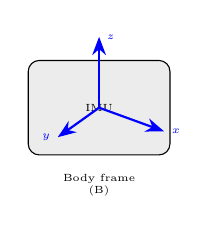
\begin{tikzpicture}[font=\tiny, scale=0.75, transform shape]
      \draw[fill=gray!15, rounded corners] (-1.2,-0.8) rectangle (1.2,0.8);
      \node at (0,0) {IMU};
      \draw[-Stealth, blue, thick] (0,0) -- (0,1.2) node[right]{$z$};
      \draw[-Stealth, blue, thick] (0,0) -- (1.1,-0.4) node[right]{$x$};
      \draw[-Stealth, blue, thick] (0,0) -- (-0.7,-0.5) node[left]{$y$};
      \node[below, align=center] at (0,-1.0) {Body frame\\(B)};
    \end{tikzpicture}
    \end{center}
  \end{columns}
\end{frame}

% ---------- 4
\begin{frame}{IMU 측정 모델 — 핵심 방정식}
  \begin{block}{가속도계}
    \[
      \bm{a}_m \;=\; \underbrace{\bm{R}^\top(\bm{a}_W - \bg_W)}_{\text{진짜 비중력 가속도 (Body frame)}}
      \;+\; \underbrace{\bm{b}_a}_{\text{바이어스}}
      \;+\; \underbrace{\bm{n}_a}_{\text{화이트 노이즈}}
    \]
    \scriptsize ($\bm{a}_W$: World frame 운동 가속도, $\bg_W$: World frame 중력. ENU/NED 모두 가능, 부호만 일관)
  \end{block}
  \begin{block}{자이로스코프}
    \[
      \bomega_m \;=\; \underbrace{\bomega}_{\text{진짜 각속도}}
      \;+\; \underbrace{\bm{b}_g}_{\text{바이어스}}
      \;+\; \underbrace{\bm{n}_g}_{\text{화이트 노이즈}}
    \]
  \end{block}
  \pause
  \vspace{0.2em}
  \textbf{de-biased 측정값} (바이어스 추정치로 보정):
  \[
    \atil \;=\; \bm{a}_m - \hatba, \qquad
    \omegatil \;=\; \bomega_m - \hatbg
  \]
\end{frame}

% ---------- 5
\begin{frame}{바이어스 모델 — 임의 보행}
  바이어스는 \emph{느리게 변하는} 확률 과정으로 모델링:
  \[
    \dot{\bm{b}}_g = \bm{n}_{bg}, \quad
    \dot{\bm{b}}_a = \bm{n}_{ba}
  \]
  $\bm{n}_{bg}, \bm{n}_{ba}$: 화이트 노이즈 (분산 $\sigma_{bg}^2, \sigma_{ba}^2$)
  \vspace{0.4em}
  \begin{columns}
    \column{0.5\textwidth}
    \begin{block}{결과}
      바이어스는 \textbf{적분된 노이즈}\\
      = Brownian motion\\
      = ESKF 상태로 추정 가능
    \end{block}
    \column{0.45\textwidth}
    \footnotesize
    \textbf{이산화} ($\Delta t$):
    \[
      \bm{b}_{k+1} \approx \bm{b}_k + \bm{n}_{bg}\,\Delta t
    \]
    분산: $\sigma^2_{\text{disc}} = \sigma^2_{bg}\,\Delta t$
  \end{columns}
  \pause
  \vspace{0.3em}
  \begin{alertblock}{왜 ESKF가 바이어스를 추정할 수 있는가}
    KF는 위치 측정 정보가 들어올 때, 공분산 교차항 $\bP_{p,b}$를 통해 바이어스 오차를 역방향으로 업데이트.
  \end{alertblock}
\end{frame}

% ---------- 6
\begin{frame}{노이즈 파라미터 — IMU Datasheet에서 읽기}
  \begin{center}\footnotesize
  \begin{tabular}{lll}
    \toprule
    파라미터 & 기호 & 단위 \\
    \midrule
    Gyro 각도 랜덤 보행 (ARW) & $\sigma_g$ & deg/s/$\sqrt{\text{Hz}}$ 또는 rad/s/$\sqrt{\text{Hz}}$ \\
    Gyro 바이어스 불안정성  & $\sigma_{bg}$ & deg/hr \\
    Accel 속도 랜덤 보행 (VRW) & $\sigma_a$ & m/s²/$\sqrt{\text{Hz}}$ \\
    Accel 바이어스 불안정성 & $\sigma_{ba}$ & $\mu g$ 또는 m/s² \\
    \bottomrule
  \end{tabular}
  \end{center}
  \pause
  \vspace{0.3em}
  \begin{block}{Allan Deviation}
    로그-로그 그래프에서 기울기 $-1/2$ 구간 = 화이트 노이즈 ($\sigma_g, \sigma_a$)\\
    기울기 $0$ 구간 = 바이어스 불안정성 ($\sigma_{bg}, \sigma_{ba}$)\\
    기울기 $+1/2$ 구간 = 속도/각도 랜덤 보행 (더 장기 드리프트)
  \end{block}
  \vspace{0.2em}
  OpenVINS 파라미터 예: \texttt{gyroscope\_noise\_density: 1.6968e-04}, \texttt{gyroscope\_random\_walk: 1.9393e-05}
\end{frame}

% ---------- 7
\begin{frame}{명목 상태 연속시간 동역학}
  IMU 측정값으로 명목 상태를 전파:
  \begin{align*}
    \dot{\hatp} &= \hatv \\[2pt]
    \dot{\hatv} &= \hatR\,\atil + \bg \quad\text{(중력 World frame으로 더함)} \\[2pt]
    \dot{\hatR} &= \hatR\,\skewx{\omegatil} \\[2pt]
    \dot{\hat{\bm{b}}}_g &= 0 \\[2pt]
    \dot{\hat{\bm{b}}}_a &= 0
  \end{align*}
\end{frame}

% ---------- 7b
\begin{frame}{명목 상태 이산화 (Euler)}
  연속시간 동역학을 $\Delta t$ 간격으로 적분:
  \begin{align*}
    \hatv_{k+1} &= \hatv_k + (\hatR_k\,\atil_k + \bg)\,\Delta t \\[2pt]
    \hatp_{k+1} &= \hatp_k + \hatv_k\,\Delta t + \tfrac{1}{2}(\hatR_k\,\atil_k+\bg)\Delta t^2 \\[2pt]
    \hatR_{k+1} &= \hatR_k\,\Exp(\omegatil_k\,\Delta t)
  \end{align*}
  \pause
  \vspace{0.3em}
  \begin{block}{실제 구현}
    실제 코드는 Runge-Kutta 4차 사용 (더 정확). OpenVINS: \texttt{Propagator.cpp}.
  \end{block}
\end{frame}

% ---------- 8
\begin{frame}[shrink=10]{오차 상태 동역학 유도 — $\dphivec$}
  진짜 회전: $\bm{R} = \hatR\,\Exp(\dphivec)$.\;
  엄밀히 $\frac{d}{dt}\Exp(\dphivec) = \Exp(\dphivec)\,\skewx{J_r(\dphivec)\,\dot{\dphivec}}$.

  \vspace{0.2em}
  \textbf{사용하는 두 근사} (small $\dphivec$): \;\;
  (i) $\Exp(\dphivec) \approx \bI$, \;\;
  (ii) $J_r(\dphivec) \approx \bI$.
  \[
    \dot{\bm{R}} = \hatR\,\skewx{\omegatil}\,\Exp(\dphivec) + \hatR\,\Exp(\dphivec)\skewx{J_r\dot{\dphivec}}
    \;\overset{(i),(ii)}{\approx}\; \hatR\,\skewx{\omegatil} + \hatR\,\skewx{\dot{\dphivec}}
  \]
  진짜 회전 방정식:
  \[
    \dot{\bm{R}} = \bm{R}\,\skewx{\bomega_\text{true}} = \hatR\,\skewx{\bomega_\text{true}}
    = \hatR\,\skewx{\omegatil - \dbgvec - \bm{n}_g}
  \]
  \pause
  같다고 놓으면:
  \[
    \hatR\,\skewx{\omegatil} + \hatR\,\skewx{\dot{\dphivec}}
    = \hatR\,\skewx{\omegatil} - \hatR\,\skewx{\dbgvec} - \hatR\,\skewx{\bm{n}_g}
  \]
  \[
    \boxed{\dot{\dphivec} = -\skewx{\omegatil}\,\dphivec - \dbgvec - \bm{n}_g}
  \]
\end{frame}

% ---------- 9
\begin{frame}{오차 상태 동역학 유도 — $\dvvec$}
  진짜 속도 미분:
  \[
    \dot{\bm{v}} = \bm{R}\bm{a}_\text{true} + \bg = \bm{R}(\atil - \dbavec - \bm{n}_a) + \bg
  \]
  명목 속도 미분:
  \[
    \dot{\hatv} = \hatR\,\atil + \bg
  \]
  \pause
  차이:
  \begin{align*}
    \dot{\dvvec} &= \dot{\bm{v}} - \dot{\hatv}
    = \bm{R}(\atil-\dbavec-\bm{n}_a) - \hatR\,\atil \\
    &\approx (\hatR + \hatR\skewx{\dphivec})(\atil-\dbavec-\bm{n}_a) - \hatR\,\atil \\
    &= \hatR\skewx{\dphivec}\,\atil - \hatR\,\dbavec - \hatR\,\bm{n}_a \\
    &= -\hatR\skewx{\atil}\,\dphivec - \hatR\,\dbavec - \hatR\,\bm{n}_a
  \end{align*}
  \[
    \boxed{\dot{\dvvec} = -\hatR\skewx{\atil}\,\dphivec - \hatR\,\dbavec - \hatR\,\bm{n}_a}
  \]
\end{frame}

% ---------- 10
\begin{frame}[shrink=5]{연속시간 F, G 행렬 (15×15, 15×12)}
  \textbf{상태 순서}: $\dxvec = [\dphivec,\,\dpvec,\,\dvvec,\,\dbgvec,\,\dbavec]^\top$
  \[
    \bF = \begin{pmatrix}
      -\skewx{\omegatil} & 0 & 0 & -\bI & 0 \\
       0                 & 0 & \bI & 0   & 0 \\
      -\hatR\skewx{\atil}& 0 & 0 &  0   & -\hatR \\
       0 & 0 & 0 & 0 & 0 \\
       0 & 0 & 0 & 0 & 0
    \end{pmatrix}
  \]
  \textbf{노이즈 순서}: $\bm{n} = [\bm{n}_g, \bm{n}_a, \bm{n}_{bg}, \bm{n}_{ba}]^\top \in \R^{12}$
  \[
    \bm{G} = \begin{pmatrix}
      -\bI & 0 & 0 & 0 \\
       0 & 0 & 0 & 0 \\
       0 & -\hatR & 0 & 0 \\
       0 & 0 & \bI & 0 \\
       0 & 0 & 0 & \bI
    \end{pmatrix}
  \]
\end{frame}

% ---------- 11
\begin{frame}{이산화 — Euler vs 행렬 지수}
  \textbf{1차 Euler 이산화}:
  \[
    \bF_d \approx \bI + \bF\,\Delta t
  \]
  \[
    \bQ_d \approx \bm{G}\,\bQ_c\,\bm{G}^\top\,\Delta t
  \]
  \pause
  \vspace{0.3em}
  \textbf{2차 Cayley-Hamilton (Van Loan 방법)}:
  \[
    \bF_d \approx \bI + \bF\,\Delta t + \tfrac{1}{2}\bF^2\,\Delta t^2
  \]
  \[
    \bQ_d = \int_0^{\Delta t} e^{\bF\tau}\bm{G}\bQ_c\bm{G}^\top e^{\bF^\top\tau}\,d\tau
  \]
  \pause
  \begin{block}{실용적 선택}
    IMU 100Hz, $\Delta t = 0.01$s일 때 1차 Euler로 충분한 경우 많음. \\
    OpenVINS는 고차 근사 사용 (Xi\_1..Xi\_4).
  \end{block}
\end{frame}

% ---------- 12
\begin{frame}[fragile]{OpenVINS Propagator — 이산 Qd 계산}
  \texttt{ov\_msckf/src/update/Propagator.cpp}
\begin{lstlisting}[language=C++, basicstyle=\ttfamily\tiny]
// Continuous noise covariance (12x12): [n_g, n_ba, n_bg, n_a] order
Eigen::MatrixXd Qc = Eigen::MatrixXd::Zero(12,12);
Qc.block(0,0,3,3) = pow(imu_data.gyro_noise,2)*Eigen::Matrix3d::Identity();
Qc.block(3,3,3,3) = pow(imu_data.accel_noise,2)*Eigen::Matrix3d::Identity();
Qc.block(6,6,3,3) = pow(imu_data.gyro_walk,2)*Eigen::Matrix3d::Identity();
Qc.block(9,9,3,3) = pow(imu_data.accel_walk,2)*Eigen::Matrix3d::Identity();

// Discrete Qd using Van Loan / higher-order Taylor
// Xi_1 = I*dt + 0.5*F_33*dt^2 + ...  (computed analytically)
Qd = G * Qc * G.transpose() * dt;  // simplified; code uses Xi matrices
\end{lstlisting}
  \vspace{0.2em}
  {\footnotesize 출처: \url{github.com/rpng/open_vins} — \texttt{Propagator.cpp}, GPLv3 라이선스}

  \vspace{0.2em}
  연속 잡음 밀도 $\sigma_g^2$ → 이산 분산 $\sigma_g^2/\Delta t$ (샘플링 스펙 확인 필요).
\end{frame}

% ---------- 13
\begin{frame}[shrink=10]{ESKF Predict — 전체 알고리즘}
  IMU 측정 $(\bomega_m, \bm{a}_m)$이 도착할 때마다:
  \begin{enumerate}
    \item $\omegatil = \bomega_m - \hatbg$, \;$\atil = \bm{a}_m - \hatba$
    \item \textbf{명목 상태 적분} (Euler 또는 RK4):
      \begin{align*}
        \hatv &\leftarrow \hatv + (\hatR\,\atil + \bg)\,\Delta t \\
        \hatp &\leftarrow \hatp + \hatv\,\Delta t \\
        \hatR &\leftarrow \hatR\,\Exp(\omegatil\,\Delta t)
      \end{align*}
    \item \textbf{F, G 계산} ($\hatR, \atil, \omegatil$ 사용)
    \item \textbf{이산 $\bF_d, \bQ_d$ 계산}
    \item \textbf{공분산 전파}: $\bP \leftarrow \bF_d\bP\bF_d^\top + \bQ_d$
  \end{enumerate}
  \pause
  \begin{alertblock}{주의}
    명목 상태 업데이트(2번)는 \emph{비선형}이고, 공분산 전파(5번)는 \emph{선형}이다. \\
    이 분리가 ESKF의 핵심이다.
  \end{alertblock}
\end{frame}

% ---------- 14
\begin{frame}{IMU 등급 — MEMS vs 전술급}
  \begin{center}\footnotesize
  \begin{tabular}{lccc}
    \toprule
    등급 & ARW (deg/$\sqrt{\text{hr}}$) & 바이어스 안정성 (deg/hr) & 대표 예시 \\
    \midrule
    소비자 MEMS & $> 0.5$ & $> 100$ & MPU-9250, ICM-42688 \\
    산업용 MEMS & $0.1$--$0.5$ & $10$--$100$ & BMI088, ADIS16470 \\
    전술급 & $0.01$--$0.1$ & $1$--$10$ & Analog Devices ADIS16505 \\
    항법급 (RLG/FOG) & $< 0.01$ & $< 0.1$ & HG1700, iXblue \\
    \bottomrule
  \end{tabular}
  \end{center}
  \pause
  \vspace{0.2em}
  \begin{block}{의미}
    MEMS IMU + GPS 없이 순수 적분(Dead reckoning):
    1분 후 위치 오차 $\sim$ 100m (소비자급) vs. $\sim$ 1m (전술급). \\
    그래서 GNSS/카메라/LiDAR 보정이 필수.
  \end{block}
\end{frame}

% ---------- 15
\begin{frame}[shrink=8]{IMU Preintegration 개념 (Forster 2017)}
  \textbf{문제}: 카메라 두 keyframe 사이에 IMU가 100개 → F를 100번 곱해야 하는가?

  \textbf{해법}: \emph{Preintegration} — IMU 측정을 한 번에 ``요약''
  \begin{align*}
    \Delta\bm{R}_{ij} &= \prod_{k=i}^{j-1} \Exp(\omegatil_k\,\Delta t) \\
    \Delta\bm{v}_{ij} &= \sum_{k=i}^{j-1} \Delta\bm{R}_{ik}\,\atil_k\,\Delta t \\
    \Delta\bm{p}_{ij} &= \sum_{k=i}^{j-1} \!\left(\Delta\bm{v}_{ik}\,\Delta t
                        + \tfrac{1}{2}\Delta\bm{R}_{ik}\,\atil_k\,\Delta t^2\right)
  \end{align*}
  \pause
  \begin{block}{핵심 이점}
    $\Delta\bm{R}_{ij}, \Delta\bm{v}_{ij}, \Delta\bm{p}_{ij}$는 \emph{바이어스만 바뀌면 선형 보정}으로 재계산 가능.\\
    GTSAM factor graph에서 IMU factor로 직접 사용 (Forster, RSS 2015).
  \end{block}
\end{frame}

% ---------- 16
\begin{frame}[fragile]{VINS-Mono midPointIntegration — 바이어스 보정 구조}
  \texttt{estimator/src/factor/integration\_base.h}
\begin{lstlisting}[language=C++, basicstyle=\ttfamily\tiny]
void midPointIntegration(double dt,
    const Vector3d &acc_0, const Vector3d &gyr_0,
    const Vector3d &acc_1, const Vector3d &gyr_1,
    const Vector3d &delta_p,    // preintegrated p
    const Quaterniond &delta_q, // preintegrated q
    const Vector3d &delta_v,    // preintegrated v
    const Vector3d &linearized_ba,
    const Vector3d &linearized_bg,
    Vector3d &result_delta_p, ...)
{
    Vector3d w_x = 0.5 * (gyr_0 + gyr_1) - linearized_bg;  // de-biased
    Vector3d a_x = 0.5 * (acc_0 + acc_1) - linearized_ba;  // de-biased
    // ... F, V matrix build + covariance propagation
}
\end{lstlisting}
  {\footnotesize 출처: \url{github.com/HKUST-Aerial-Robotics/VINS-Mono} — GPL-3.0}
  \vspace{0.1em}

  mid-point 적분 = IMU 두 sample의 평균을 한 step에 적분 (RK2 수준 정확도).
\end{frame}

% ---------- 17
\begin{frame}{중력 벡터 — World frame과 Body frame}
  \begin{itemize}
    \item World frame (NED): $\bg = (0, 0, g)^\top$, $g \approx 9.81$ m/s²
    \item World frame (ENU): $\bg = (0, 0, -g)^\top$
    \item 가속도계는 \emph{Body frame}에서 측정:
      $\bm{a}_m = \hatR^\top(\bm{a}_\text{World} - \bg) + \bm{b}_a + \bm{n}_a$
  \end{itemize}
  \pause
  \vspace{0.3em}
  \begin{alertblock}{흔한 실수}
    명목 전파식 $\dot{\hatv} = \hatR\,\atil + \bg$에서 \\
    $\bg$의 부호와 좌표계가 World frame인지 확인하지 않으면 발산.\\
    OpenVINS는 ENU: $\bg = [0,0,-9.81]$.
  \end{alertblock}
  \pause
  \vspace{0.2em}
  \begin{block}{자기 보정 (self-calibration)}
    초기 정지 상태에서 $\bm{a}_m \approx -\hatR^\top\bg$ → $\hatR_0$ 추정 가능.\\
    ``정렬 단계''(alignment phase)라고 부른다.
  \end{block}
\end{frame}

% ---------- 18
\begin{frame}{이번 회차 핵심 다섯 개}
  \begin{enumerate}
    \item 측정 모델: $\bm{a}_m = \hatR^\top(\bm{a}-\bg)+\bm{b}_a+\bm{n}_a$, \;$\bomega_m = \bomega+\bm{b}_g+\bm{n}_g$
    \item F 행렬 $\dot{\dphivec} = -\skewx{\omegatil}\dphivec - \dbgvec$,
          $\dot{\dvvec} = -\hatR\skewx{\atil}\dphivec - \hatR\dbavec$ 유도
    \item G 행렬: 연속 노이즈를 오차 상태로 이어주는 경로
    \item 이산화: $\bF_d \approx \bI + \bF\Delta t$, $\bQ_d \approx \bm{G}\bQ_c\bm{G}^\top\Delta t$
    \item Preintegration: 카메라 keyframe 사이 IMU를 한 번에 요약
  \end{enumerate}
  \vspace{0.3em}
  \begin{block}{한 줄 요약}
    IMU는 잡음+바이어스가 섞인 센서. ESKF는 그 오차를 \emph{선형 KF}로 추적하며 보정한다.
  \end{block}
\end{frame}

% ---------- 19
\begin{frame}{과제 5 (다음 시간 전)}
  \begin{enumerate}
    \item 슬라이드 8의 $\dot{\dphivec}$ 유도를 종이에 재현. 특히
          $\skewx{\dphivec}\,\skewx{\omegatil} \approx 0$ 근사가 어디서 쓰였는지 표시.
    \item 슬라이드 9의 $\dot{\dvvec}$ 유도에서 $\bm{R} \approx \hatR(\bI+\skewx{\dphivec})$
          근사의 오차 크기를 $\|\dphivec\|^2$ 관점에서 추정.
    \item (선택) MPU-9250 또는 BMI088 datasheet에서 gyro ARW와 bias instability를 찾아
          ESKF $\bQ_c$ 파라미터로 변환.
    \item (선택) OpenVINS \texttt{Propagator.cpp}의 \texttt{compute\_F\_and\_G\_analytic()}를
          읽고, 슬라이드 10의 F 행렬 각 블록과 대응 관계를 코멘트로 표시.
  \end{enumerate}
\end{frame}

% ---------- 20
\begin{frame}{다음 시간 예고 — 6회차: 멀티센서 Update}
  \textbf{GPS, 휠 인코더, 카메라 측정을 ESKF에 어떻게 넣는가}
  \begin{itemize}
    \item 일반 Update 공식: $\bz = h(\hatx) + \bH\,\dxvec + \bm{v}$
    \item GPS: $\bH_\text{GPS} = [0,\,\bI,\,0,\,0,\,0]$ (위치 측정)
    \item 휠 속도: $\bH_\text{wheel}$ 유도 (body frame velocity)
    \item 카메라 피처 잔차: OpenVINS MSCKF H matrix
    \item Mahalanobis 기반 이상값 제거 (outlier rejection)
  \end{itemize}
  \vspace{0.3em}
  \begin{block}{미리 생각해볼 것}
    GPS는 World frame 위치를 준다. Body frame 속도만 주는 휠 인코더와 어떻게 합치는가?
  \end{block}
\end{frame}

% ---------- 21
\begin{frame}
  \vspace{1.5cm}
  \begin{center}
    {\Huge \textbf{질문 환영}}\\[1em]
    \large IMU를 이해하면 ESKF Predict의 절반이 끝난다
  \end{center}
\end{frame}

% =================================
% ========== L5 확장: Preintegration Jacobians (Forster 2017) ==========
% 이 파일은 lecture05_imu.tex 뒤에 \input{} 으로 삽입하거나
% 독립적으로 컴파일 가능한 Beamer 프레임 모음입니다.
% 의존 매크로: preamble.tex (SOthree, SEthree, Exp, Log, skewx,
%   hatR, hatp, hatv, hatbg, hatba, dxvec, dphivec, dpvec, dvvec,
%   dbgvec, dbavec, atil, omegatil, bP, bQ, bR, bF, bH, bK, bI,
%   bx, bz, bg, ba, bomega, bphi, bn, R)

% ──────────────────────────────────────────────────────────────────────
%  섹션 타이틀 프레임
% ──────────────────────────────────────────────────────────────────────

% ---------- PI-0
\begin{frame}{}
  \begin{center}
    \vspace{2em}
    {\Large\bfseries Part II}\\[0.6em]
    {\LARGE\bfseries Preintegration Jacobians}\\[0.4em]
    {\large Forster 2017 TRO 완전 유도}\\[1.5em]
    \begin{tikzpicture}
      \draw[thick, mDarkTeal, rounded corners=4pt]
        (-4.2,-0.5) rectangle (4.2,0.5);
      \node[font=\small] at (0,0) {%
        바이어스 Jacobian $\cdot$ 공분산 전파 $\cdot$ Factor Residual};
    \end{tikzpicture}
  \end{center}
\end{frame}

% ──────────────────────────────────────────────────────────────────────
%  PI-1  왜 Jacobian이 필요한가
% ──────────────────────────────────────────────────────────────────────

% ---------- PI-1
\begin{frame}{Preintegration 재방문 — 왜 Jacobian이 필요한가}

  \textbf{기존 문제:} 바이어스 추정이 업데이트되면 $\Delta$를 처음부터 재적분해야 함.

  \pause
  \vspace{0.4em}
  \begin{columns}
    \column{0.5\textwidth}
    \begin{alertblock}{비용}
      키프레임 사이 수백 개의 IMU 샘플\\
      $\Rightarrow$ 매 업데이트마다 $O(N)$ 재적분\\
      $\Rightarrow$ 실시간 불가
    \end{alertblock}

    \column{0.46\textwidth}
    \begin{exampleblock}{해법 (Forster 2017)}
      바이어스 변화 $\delta b$에 대한\\
      \textbf{1차 Taylor 근사}로 선형 보정\\
      $\Rightarrow$ 재적분 없음
    \end{exampleblock}
  \end{columns}

  \pause
  \vspace{0.5em}
  \begin{block}{핵심 근사식}
    \begin{align*}
      \Delta R_{ij}(b_g + \delta b_g)
        &\approx \Delta R_{ij}(b_g)\;\Exp\!\bigl(J_{b_g}^{\Delta R}\,\delta b_g\bigr)\\[4pt]
      \Delta v_{ij}(b + \delta b)
        &\approx \Delta v_{ij}(b)
          + J_{b_g}^{\Delta v}\,\delta b_g
          + J_{b_a}^{\Delta v}\,\delta b_a\\[4pt]
      \Delta p_{ij}(b + \delta b)
        &\approx \Delta p_{ij}(b)
          + J_{b_g}^{\Delta p}\,\delta b_g
          + J_{b_a}^{\Delta p}\,\delta b_a
    \end{align*}
  \end{block}

  \pause
  \vspace{0.2em}
  \begin{alertblock}{목표}
    이 \textbf{6개의 Jacobian 행렬}을 preintegration 동안 재귀적으로 같이 적분한다.
  \end{alertblock}
\end{frame}

% ──────────────────────────────────────────────────────────────────────
%  PI-2  이산 시간 preintegration 복습
% ──────────────────────────────────────────────────────────────────────

% ---------- PI-2
\begin{frame}[shrink=10]{이산 시간 Preintegration 복습}

  두 키프레임 $i,j$ 사이에 $N = j - i$개의 IMU 샘플이 있다고 하자.

  \begin{block}{Preintegrated Measurements}
    \begin{align*}
      \Delta R_{ij}
        &= \prod_{k=i}^{j-1}\Exp\!\bigl(\omegatil_k\,\Delta t\bigr)
        \;\in\;\SOthree \\[6pt]
      \Delta v_{ij}
        &= \sum_{k=i}^{j-1}\Delta R_{ik}\;\atil_k\,\Delta t
        \;\in\;\R^3 \\[6pt]
      \Delta p_{ij}
        &= \sum_{k=i}^{j-1}\!\left(\Delta v_{ik}\,\Delta t
            + \tfrac{1}{2}\,\Delta R_{ik}\;\atil_k\,\Delta t^2\right)
        \;\in\;\R^3
    \end{align*}
  \end{block}

  \pause
  \vspace{0.3em}
  \textbf{de-biased 측정값:}
  \[
    \omegatil_k = \bomega_{m,k} - b_g,
    \qquad
    \atil_k = \bm{a}_{m,k} - b_a
  \]

  \pause
  \begin{exampleblock}{재귀 관계 (한 스텝 전진)}
    \[
      \Delta R_{i,k+1} = \Delta R_{ik}\;\Exp(\omegatil_k\Delta t),
      \quad
      \Delta v_{i,k+1} = \Delta v_{ik} + \Delta R_{ik}\;\atil_k\,\Delta t
    \]
  \end{exampleblock}

  \vspace{0.2em}
  \footnotesize 참고: $\Delta R_{ii} = I,\; \Delta v_{ii} = \bm{0},\; \Delta p_{ii} = \bm{0}$
\end{frame}

% ──────────────────────────────────────────────────────────────────────
%  PI-3  Noise 모델: 연속 → 이산
% ──────────────────────────────────────────────────────────────────────

% ---------- PI-3
\begin{frame}[shrink=15]{Noise 모델: IMU 연속 시간 $\to$ 이산 시간}

  \begin{alertblock}{\small 이 강의의 부호 컨벤션 (이후 모든 슬라이드에 일관 적용)}
    \footnotesize
    \[
      \bomega_m = \bomega + b_g + \bm{n}_g,\qquad
      \bm{a}_m = \bm{R}^\top(\bm{a}_W - \bm{g}_W) + b_a + \bm{n}_a
    \]
    노이즈가 \textbf{측정값에 더해지는} 형태. 따라서 ``bias-제거된 추정치''
    $\omegatil = \bomega_m - b_g$는 참값보다 \emph{$\bm{n}_g$만큼 큰} 값:
    $\bomega = \omegatil - \bm{n}_g$.\\
    이 부호 규약 때문에 후속 유도(PI-21/22)에서 $B_k$에 \textbf{음의 부호}가 자연스럽게 등장한다.
  \end{alertblock}

  \pause
  \vspace{0.4em}
  \begin{block}{이산화 ($\Delta t$ 적분 후)}
    \[
      \bm{\eta}_d^g \sim \mathcal{N}\!\left(0,\;\frac{\sigma_g^2}{\Delta t}I\right),
      \qquad
      \bm{\eta}_d^a \sim \mathcal{N}\!\left(0,\;\frac{\sigma_a^2}{\Delta t}I\right)
    \]
    바이어스 임의 보행 이산화:
    \[
      \bm{\eta}_{bg} \sim \mathcal{N}(0,\,\sigma_{bg}^2\Delta t\,I),
      \qquad
      \bm{\eta}_{ba} \sim \mathcal{N}(0,\,\sigma_{ba}^2\Delta t\,I)
    \]
  \end{block}

  \pause
  \begin{block}{이산 노이즈 행렬 $Q_d \in \R^{12\times 12}$}
    \[
      Q_d = \mathrm{diag}\!\left(
        \frac{\sigma_g^2}{\Delta t}I_3,\;
        \frac{\sigma_a^2}{\Delta t}I_3,\;
        \sigma_{bg}^2\Delta t\,I_3,\;
        \sigma_{ba}^2\Delta t\,I_3
      \right)
    \]
    순서: gyro noise $|$ accel noise $|$ gyro RW $|$ accel RW
  \end{block}

  \pause
  \begin{exampleblock}{OpenVINS 파라미터 대응}
    \texttt{gyroscope\_noise\_density} $\to \sigma_g$,\quad
    \texttt{accelerometer\_noise\_density} $\to \sigma_a$\\
    \texttt{gyroscope\_random\_walk} $\to \sigma_{bg}$,\quad
    \texttt{accelerometer\_random\_walk} $\to \sigma_{ba}$
  \end{exampleblock}

  \pause
  \begin{alertblock}{\small PSD 컨벤션 두 가지 — 데이터시트 단위에 \emph{매번} 확인 필수}
    \footnotesize
    \begin{tabular}{ll}
      \toprule
      \textbf{컨벤션} & \textbf{이산 분산} \\
      \midrule
      Continuous PSD ($\sigma_g$ 단위 = $\text{rad/s}/\sqrt{\text{Hz}}$) & $\sigma_g^2 / \Delta t$ \\
      Discrete (이미 $\Delta t$ 적분, $\sigma_g^d$ 단위 = $\text{rad/s}$) & $(\sigma_g^d)^2$ \\
      Allan variance (deg/$\sqrt{\text{h}}$ 등) & 단위 변환 후 위 식 사용 \\
      \bottomrule
    \end{tabular}\\[2pt]
    \textbf{이 강의는 Continuous PSD 컨벤션}을 사용한다 (OpenVINS, Kalibr, EuRoC 데이터셋과 일치).
    Forster 2017 / VINS-Mono도 PSD 컨벤션이지만, 일부 코드는 이미 $\sigma_g \cdot \sqrt{\Delta t}$ 형태로 받기도 하니 \emph{IMU 캘리브레이션의 1순위 디버깅 포인트}.
  \end{alertblock}
\end{frame}

% ──────────────────────────────────────────────────────────────────────
%  PI-4  공분산 전파 재귀식
% ──────────────────────────────────────────────────────────────────────

% ---------- PI-4
\begin{frame}[shrink=20]{Preintegration 공분산 전파 — 재귀식}

  \textbf{상태:} 스텝 $k$ 에서 (frame $i$에 상대적인)
  \[
    \bm{\xi}_k = \bigl(\delta\bm{\phi}_k,\;\delta v_k,\;\delta p_k\bigr) \in \R^9
  \]
  (회전 오차 $\delta\phi \in \R^3$, 속도 오차 $\delta v \in \R^3$, 위치 오차 $\delta p \in \R^3$)

  \pause
  \vspace{0.4em}
  \begin{block}{선형화 오차 동역학 (한 스텝)}
    \[
      \bm{\xi}_{k+1} = A_k\,\bm{\xi}_k + B_k\,\bm{\eta}_k
    \]
    \begin{itemize}
      \item $A_k \in \R^{9\times 9}$: 오차 상태 전이 행렬
      \item $B_k \in \R^{9\times 12}$: 노이즈 입력 행렬
      \item $\bm{\eta}_k \in \R^{12}$: $[\bm{\eta}_g^\top,\,\bm{\eta}_a^\top,\,\bm{\eta}_{bg}^\top,\,\bm{\eta}_{ba}^\top]^\top$
    \end{itemize}
  \end{block}

  \pause
  \begin{alertblock}{공분산 재귀 전파}
    \[
      \boxed{\Sigma_{k+1} = A_k\,\Sigma_k\,A_k^\top + B_k\,Q_d\,B_k^\top}
    \]
    초기 조건: $\Sigma_{ii} = 0_{9\times 9}$
  \end{alertblock}

  \pause
  \vspace{0.2em}
  이 식을 $k = i$ 부터 $k = j-1$ 까지 반복하면 $\Sigma_{ij} \in \R^{9\times 9}$ 획득.
\end{frame}

% ──────────────────────────────────────────────────────────────────────
%  PI-5  A_k 행렬 — 회전 부분
% ──────────────────────────────────────────────────────────────────────

% ---------- PI-5
\begin{frame}[shrink=10]{$A_k$ 행렬 유도 — 회전 오차 부분}

  명목 회전 전파:
  \[
    \Delta R_{i,k+1} = \Delta R_{ik}\;\Exp(\omegatil_k\Delta t)
  \]
  실제 회전 (노이즈 포함):
  \[
    \Delta \tilde{R}_{i,k+1}
    = \Delta R_{ik}\;\Exp\!\bigl((\omegatil_k - \bm{\eta}_g)\Delta t\bigr)
  \]

  \pause
  오차 정의: $\Delta R_{ik} = \Delta\tilde{R}_{ik}\;\Exp(-\delta\phi_k)$. BCH 근사를 적용하면:

  \begin{block}{회전 오차 전파}
    \[
      \delta\phi_{k+1}
      = \Exp\!\bigl(-\omegatil_k\Delta t\bigr)\,\delta\phi_k
        \;+\; J_r^{-1}(\omegatil_k\Delta t)\,\Delta t\;\bm{\eta}_g
    \]
  \end{block}

  \pause
  따라서 $A_k$의 회전 블록:
  \[
    A_k[0\!:\!3,\;0\!:\!3]
    = \Exp\!\bigl(-\omegatil_k\Delta t\bigr)
    \;\approx\; I - \skewx{\omegatil_k}\Delta t
  \]

  \pause
  \begin{alertblock}{$J_r^{-1}$가 여기서 처음으로 등장하는 이유}
    BCH 공식에서 두 회전의 합성 오차를 선형화할 때 Right Jacobian의 역행렬이 자연스럽게 나타남.
    $J_r(\bm{\phi}) = I - \frac{1-\cos\|\bm{\phi}\|}{\|\bm{\phi}\|^2}\skewx{\bm{\phi}}
    + \frac{\|\bm{\phi}\|-\sin\|\bm{\phi}\|}{\|\bm{\phi}\|^3}\skewx{\bm{\phi}}^2$
    (작은 각도: $J_r \approx I - \frac{1}{2}\skewx{\bm{\phi}}$)
  \end{alertblock}
\end{frame}

% ──────────────────────────────────────────────────────────────────────
%  PI-6  A_k 행렬 — 속도/위치 부분 + 전체 구조
% ──────────────────────────────────────────────────────────────────────

% ---------- PI-6
\begin{frame}[shrink=10]{$A_k$ 행렬 유도 — 속도/위치 부분 + 전체 구조}

  \textbf{속도 오차 전파:} $\Delta v_{i,k+1} = \Delta v_{ik} + \Delta R_{ik}\atil_k\Delta t$ 선형화
  \[
    \delta v_{k+1}
    = \delta v_k
      - \Delta R_{ik}\skewx{\atil_k}\delta\phi_k\,\Delta t
  \]

  \textbf{위치 오차 전파:}
  \[
    \delta p_{k+1}
    = \delta p_k
      + \delta v_k\,\Delta t
      - \tfrac{1}{2}\Delta R_{ik}\skewx{\atil_k}\delta\phi_k\,\Delta t^2
  \]

  \pause
  \begin{block}{$A_k \in \R^{9\times 9}$ 전체 블록 구조}
    \[
      A_k =
      \begin{pmatrix}
        \Exp(-\omegatil_k\Delta t)          & \bm{0}         & \bm{0} \\[4pt]
        -\Delta R_{ik}\skewx{\atil_k}\Delta t & I              & \bm{0} \\[4pt]
        -\tfrac{1}{2}\Delta R_{ik}\skewx{\atil_k}\Delta t^2 & I\,\Delta t & I
      \end{pmatrix}
    \]
    행/열 순서: $(\delta\phi,\;\delta v,\;\delta p)$
  \end{block}

  \pause
  \begin{exampleblock}{직관}
    \begin{itemize}
      \item 대각: 각 상태가 자기 자신에게 직접 전달
      \item 아래 삼각: 회전 오차 $\to$ 속도/위치 오차 (cross-coupling)
      \item 선형 구조 덕분에 KF Riccati 전파 가능
    \end{itemize}
  \end{exampleblock}
\end{frame}

% ──────────────────────────────────────────────────────────────────────
%  PI-7  B_k 행렬
% ──────────────────────────────────────────────────────────────────────

% ---------- PI-7
\begin{frame}[shrink=10]{$B_k$ 행렬 — 노이즈 입력 행렬}

  $B_k \in \R^{9\times 12}$: 노이즈 벡터 $\bm{\eta} = [\bm{\eta}_g^\top, \bm{\eta}_a^\top, \bm{\eta}_{bg}^\top, \bm{\eta}_{ba}^\top]^\top$를 오차 상태로 매핑.

  \pause
  \begin{block}{블록 구조 (PI-3 부호 규약과 일관 — PI-21/22에서 엄밀 유도됨)}
    \[
      B_k =
      \begin{pmatrix}
        -J_r^{-1}(\omegatil_k\Delta t)\,\Delta t & \bm{0}                        & \bm{0} & \bm{0} \\[4pt]
        \bm{0}                                   & -\Delta R_{ik}\,\Delta t      & \bm{0} & \bm{0} \\[4pt]
        \bm{0}                                   & -\tfrac{1}{2}\Delta R_{ik}\,\Delta t^2 & \bm{0} & \bm{0}
      \end{pmatrix}
    \]
    열 순서: $(\bm{\eta}_g \mid \bm{\eta}_a \mid \bm{\eta}_{bg} \mid \bm{\eta}_{ba})$, 각 3열.
    공분산 전파 $B_k Q_d B_k^\top$에서는 부호가 $\pm$ 두 번 곱해져 \emph{사라지므로} 결과 covariance는 동일.
  \end{block}

  \pause
  \vspace{0.3em}
  \textbf{비제로 블록 설명:}
  \begin{itemize}
    \item $B_k[0\!:\!3, 0\!:\!3] = -J_r^{-1}\Delta t$:
          gyro 노이즈 $\to$ 회전 오차
    \item $B_k[3\!:\!6, 3\!:\!6] = -\Delta R_{ik}\Delta t$:
          accel 노이즈 $\to$ 속도 오차
    \item $B_k[6\!:\!9, 3\!:\!6] = -\tfrac{1}{2}\Delta R_{ik}\Delta t^2$:
          accel 노이즈 $\to$ 위치 오차
  \end{itemize}

  \pause
  \begin{alertblock}{주의: 바이어스 노이즈는 $B_k$에 없다}
    $\bm{\eta}_{bg}, \bm{\eta}_{ba}$는 바이어스 오차 상태 $\delta b_g, \delta b_a$에 직접 들어가므로,
    \textbf{별도의 bias Jacobian 방정식}으로 처리한다 (다음 슬라이드).
  \end{alertblock}
\end{frame}

% ──────────────────────────────────────────────────────────────────────
%  PI-8  ∂ΔR/∂bg 유도 (핵심)
% ──────────────────────────────────────────────────────────────────────

% ---------- PI-8
\begin{frame}[shrink=10]{$\dfrac{\partial \Delta R_{ij}}{\partial b_g}$ Jacobian 유도 — 핵심}

  \begin{block}{기호 정의}
    \[
      J_{b_g}^{\Delta R_k} \;\stackrel{\Delta}{=}\; \frac{\partial \Delta R_{ik}}{\partial b_g}
      \;\in\; \R^{3\times 3}
    \]
  \end{block}

  \pause
  $\Delta R_{i,k+1} = \Delta R_{ik}\,\Exp(\omegatil_k\Delta t)$ 에서
  $\omegatil_k = \bomega_{m,k} - b_g$ 이므로 $b_g$에 대해 미분하면:

  \begin{block}{재귀 관계 (체인룰 + BCH 근사)}
    \[
      J_{b_g}^{\Delta R_{k+1}}
      = \Exp(-\omegatil_k\Delta t)\;J_{b_g}^{\Delta R_k}
        - J_r^{-1}(\omegatil_k\Delta t)\;\Delta t
    \]
  \end{block}

  \pause
  \textbf{초기 조건:}
  \[
    J_{b_g}^{\Delta R_{ii}} = \bm{0}_{3\times 3}
    \quad (\text{frame } i \text{에서 자기 자신 = 항등원, 바이어스 의존 없음})
  \]

  \pause
  \begin{alertblock}{이 Jacobian이 preintegration Jacobian의 핵심인 이유}
    \begin{itemize}
      \item $J_{b_g}^{\Delta R}$는 속도/위치 Jacobian $J_{b_g}^{\Delta v}$, $J_{b_g}^{\Delta p}$의 \textbf{입력}이 됨
      \item 회전이 SO(3) 위에서 propagate되므로 단순한 유클리드 미분이 아님
      \item $J_r^{-1}$이 매 스텝 누적 $\Rightarrow$ 정확한 manifold 상의 Jacobian
    \end{itemize}
  \end{alertblock}
\end{frame}

% ──────────────────────────────────────────────────────────────────────
%  PI-9  ∂Δv/∂bg, ∂Δv/∂ba
% ──────────────────────────────────────────────────────────────────────

% ---------- PI-9
\begin{frame}[shrink=10]{$\dfrac{\partial \Delta v_{ij}}{\partial b_g}$,\; $\dfrac{\partial \Delta v_{ij}}{\partial b_a}$ 유도}

  \textbf{속도 재귀식 미분:}
  $\Delta v_{i,k+1} = \Delta v_{ik} + \Delta R_{ik}\,\atil_k\,\Delta t$

  \pause
  \begin{block}{$b_g$에 대한 Jacobian 재귀식}
    \[
      J_{b_g}^{\Delta v_{k+1}}
      = J_{b_g}^{\Delta v_k}
        - \Delta R_{ik}\;\skewx{\atil_k}\;J_{b_g}^{\Delta R_k}\;\Delta t
    \]
    ($\Delta R_{ik}$도 $b_g$에 의존함 $\Rightarrow$ 체인룰 필요)
  \end{block}

  \pause
  \begin{block}{$b_a$에 대한 Jacobian 재귀식}
    \[
      J_{b_a}^{\Delta v_{k+1}}
      = J_{b_a}^{\Delta v_k}
        - \Delta R_{ik}\;\Delta t
    \]
    ($\atil_k = \bm{a}_{m,k} - b_a$ 이므로 $\partial\atil_k/\partial b_a = -I$)
  \end{block}

  \pause
  \textbf{초기 조건:} $J_{b_g}^{\Delta v_{ii}} = J_{b_a}^{\Delta v_{ii}} = \bm{0}_{3\times 3}$

  \pause
  \vspace{0.2em}
  \textbf{누적 합 형태로 표현:}
  \[
    J_{b_g}^{\Delta v_{ij}}
    = -\sum_{k=i}^{j-1}\Delta R_{ik}\;\skewx{\atil_k}\;J_{b_g}^{\Delta R_{ik}}\;\Delta t,
    \qquad
    J_{b_a}^{\Delta v_{ij}}
    = -\sum_{k=i}^{j-1}\Delta R_{ik}\;\Delta t
  \]
  각각 $\R^{3\times 3}$.
\end{frame}

% ──────────────────────────────────────────────────────────────────────
%  PI-10  ∂Δp/∂bg, ∂Δp/∂ba
% ──────────────────────────────────────────────────────────────────────

% ---------- PI-10
\begin{frame}[shrink=10]{$\dfrac{\partial \Delta p_{ij}}{\partial b_g}$,\; $\dfrac{\partial \Delta p_{ij}}{\partial b_a}$ 유도}

  \textbf{위치 재귀식 미분:}
  $\Delta p_{i,k+1} = \Delta p_{ik} + \Delta v_{ik}\,\Delta t + \tfrac{1}{2}\Delta R_{ik}\,\atil_k\,\Delta t^2$

  \pause
  \begin{block}{$b_g$에 대한 Jacobian 재귀식}
    \[
      J_{b_g}^{\Delta p_{k+1}}
      = J_{b_g}^{\Delta p_k}
        + J_{b_g}^{\Delta v_k}\,\Delta t
        - \tfrac{1}{2}\,\Delta R_{ik}\;\skewx{\atil_k}\;J_{b_g}^{\Delta R_k}\;\Delta t^2
    \]
  \end{block}

  \pause
  \begin{block}{$b_a$에 대한 Jacobian 재귀식}
    \[
      J_{b_a}^{\Delta p_{k+1}}
      = J_{b_a}^{\Delta p_k}
        + J_{b_a}^{\Delta v_k}\,\Delta t
        - \tfrac{1}{2}\,\Delta R_{ik}\;\Delta t^2
    \]
  \end{block}

  \pause
  \textbf{초기 조건:} $J_{b_g}^{\Delta p_{ii}} = J_{b_a}^{\Delta p_{ii}} = \bm{0}_{3\times 3}$

  \pause
  \vspace{0.3em}
  \begin{exampleblock}{누적 합 형태}
    \begin{align*}
      J_{b_g}^{\Delta p_{ij}}
        &= \sum_{k=i}^{j-1}\!\left(
            J_{b_g}^{\Delta v_{ik}}\Delta t
            - \tfrac{1}{2}\Delta R_{ik}\skewx{\atil_k}J_{b_g}^{\Delta R_{ik}}\Delta t^2
          \right)\\[4pt]
      J_{b_a}^{\Delta p_{ij}}
        &= -\tfrac{1}{2}\sum_{k=i}^{j-1}\Delta R_{ik}\,\Delta t^2
    \end{align*}
  \end{exampleblock}

  이로써 총 \textbf{6개}의 Bias Jacobian 행렬이 완성됨.
\end{frame}

% ──────────────────────────────────────────────────────────────────────
%  PI-11  바이어스 변화 시 1차 보정 공식
% ──────────────────────────────────────────────────────────────────────

% ---------- PI-11
\begin{frame}{바이어스 변화 시 1차 보정 공식}

  ESKF update 후 바이어스 추정치가
  $b_g \to b_g + \delta b_g$,\; $b_a \to b_a + \delta b_a$\; 로 바뀌었다 하자.

  \pause
  \vspace{0.4em}
  \begin{alertblock}{Preintegration 측정값 선형 보정 (재적분 없이!)}
    \begin{align*}
      \Delta\hat{R}_{ij}
        &\approx \Delta R_{ij}\;\Exp\!\bigl(J_{b_g}^{\Delta R_{ij}}\,\delta b_g\bigr)
        \;\in\;\SOthree \\[6pt]
      \Delta\hat{v}_{ij}
        &\approx \Delta v_{ij}
          + J_{b_g}^{\Delta v_{ij}}\,\delta b_g
          + J_{b_a}^{\Delta v_{ij}}\,\delta b_a
        \;\in\;\R^3 \\[6pt]
      \Delta\hat{p}_{ij}
        &\approx \Delta p_{ij}
          + J_{b_g}^{\Delta p_{ij}}\,\delta b_g
          + J_{b_a}^{\Delta p_{ij}}\,\delta b_a
        \;\in\;\R^3
    \end{align*}
  \end{alertblock}

  \pause
  \begin{exampleblock}{계산 절감}
    \begin{itemize}
      \item 재적분: $O(N)$ matrix multiply $\times$ 업데이트 횟수
      \item 선형 보정: $O(1)$ 행렬-벡터 곱 3번
      \item Factor graph에서 매우 유용: bias 업데이트마다 호출
    \end{itemize}
  \end{exampleblock}

  \pause
  \vspace{0.2em}
  \footnotesize
  \textbf{수식 출처:} Forster \textit{et al.}, ``On-Manifold Preintegration for Real-Time
  Visual-Inertial Odometry,'' \textit{IEEE TRO} 33(1), 2017, eq.~(44)--(46).
\end{frame}

% ──────────────────────────────────────────────────────────────────────
%  PI-12  언제 선형 보정으로 충분한가
% ──────────────────────────────────────────────────────────────────────

% ---------- PI-12
\begin{frame}{언제 선형 보정으로 충분한가}

  \begin{block}{유효 조건}
    $\|\delta b_g\|$와 $\|\delta b_a\|$가 \textbf{충분히 작을 때}
    (Taylor 나머지항이 무시 가능)\\[4pt]
    구체적으로:
    \[
      \|\delta b_g\| \ll \sigma_{bg}\sqrt{T},
      \qquad
      \|\delta b_a\| \ll \sigma_{ba}\sqrt{T}
    \]
    ($T$: preintegration 구간 길이)
  \end{block}

  \pause
  \vspace{0.4em}
  \begin{columns}
    \column{0.48\textwidth}
    \begin{exampleblock}{선형 보정으로 충분한 경우}
      \begin{itemize}
        \item ESKF 업데이트 직후\\(bias 변화량 작음)
        \item 짧은 preintegration 구간
        \item 느린 운동, 낮은 바이어스 드리프트
      \end{itemize}
    \end{exampleblock}
    \column{0.48\textwidth}
    \begin{alertblock}{재적분이 필요한 경우}
      \begin{itemize}
        \item 바이어스 업데이트량이 threshold 초과
        \item 긴 구간 (수 초 이상)
        \item 격렬한 회전 운동
      \end{itemize}
    \end{alertblock}
  \end{columns}

  \pause
  \vspace{0.4em}
  \begin{block}{OpenVINS 구현 전략}
    \texttt{Propagator::repropagate()} vs \texttt{correctPropagation()}\\
    바이어스 변화량이 threshold 미만이면 보정, 초과하면 재전파.\\
    \texttt{options.dt\_slam\_delay}와 연동된 성능-정확도 trade-off.
  \end{block}
\end{frame}

% ──────────────────────────────────────────────────────────────────────
%  PI-13  Preintegration Factor — 잔차 형태
% ──────────────────────────────────────────────────────────────────────

% ---------- PI-13
\begin{frame}[shrink=10]{Preintegration Factor — 잔차 형태 (Factor Graph 연결)}

  \textbf{상태:} $\pi_i = (R_i, v_i, p_i)$,\; $\pi_j = (R_j, v_j, p_j)$,\; 바이어스 $(b_g, b_a)$.

  \pause
  \begin{block}{잔차 벡터 $\bm{r}_{ij} \in \R^9$}
    \begin{align*}
      r_{\Delta R}
        &= \Log\!\Bigl(\Delta\hat{R}_{ij}^\top\;R_i^\top\,R_j\Bigr)
        \;\in\;\R^3\\[5pt]
      r_{\Delta v}
        &= R_i^\top\!\bigl(v_j - v_i - \bg\,\Delta t_{ij}\bigr) - \Delta\hat{v}_{ij}
        \;\in\;\R^3\\[5pt]
      r_{\Delta p}
        &= R_i^\top\!\Bigl(p_j - p_i - v_i\,\Delta t_{ij} - \tfrac{1}{2}\bg\,\Delta t_{ij}^2\Bigr)
          - \Delta\hat{p}_{ij}
        \;\in\;\R^3
    \end{align*}
  \end{block}

  \pause
  여기서 $\Delta\hat{R}_{ij},\,\Delta\hat{v}_{ij},\,\Delta\hat{p}_{ij}$는 현재 바이어스에서 \textbf{선형 보정된} 값.

  \pause
  \vspace{0.2em}
  \begin{exampleblock}{Factor Graph에서의 역할}
    \begin{itemize}
      \item 잔차 $\bm{r}_{ij}$를 최소화하는 non-linear least squares
      \item $\mathcal{I}_{ij} = \Sigma_{ij}^{-1}$: 정보 행렬 (preintegration 공분산의 역)
      \item 비용함수: $\bm{r}_{ij}^\top \mathcal{I}_{ij} \bm{r}_{ij}$
      \item 이 잔차의 Jacobian에 $J_{b_g}^{\Delta R}$ 등이 등장 (다음 슬라이드)
    \end{itemize}
  \end{exampleblock}
\end{frame}

% ──────────────────────────────────────────────────────────────────────
%  PI-14  Factor Jacobian — ∂r/∂state
% ──────────────────────────────────────────────────────────────────────

% ---------- PI-14
\begin{frame}[shrink=10]{Preintegration Factor Jacobian — $\partial \bm{r} / \partial \text{state}$}

  전체 Jacobian: $\bm{J} \in \R^{9\times 24}$
  (9 residuals $\times$ 24 = state$_i$ 9 + state$_j$ 9 + bias$_i$ 6)

  \pause
  \begin{block}{$\partial r_{\Delta R} / \partial \text{state}$}
    \[
      \frac{\partial r_{\Delta R}}{\partial \delta\phi_i}
        = -\bigl(\Delta\hat{R}_{ij}^\top R_i^\top R_j\bigr)^{-\top},\quad
      \frac{\partial r_{\Delta R}}{\partial \delta\phi_j}
        = J_r^{-1}\!\left(\Log(\Delta\hat{R}_{ij}^\top R_i^\top R_j)\right),\quad
      \frac{\partial r_{\Delta R}}{\partial \delta b_g}
        = -J_r^{-1}(\cdot)\;J_{b_g}^{\Delta R_{ij}}
    \]
  \end{block}

  \pause
  \begin{block}{$\partial r_{\Delta v} / \partial \text{state}$ (대표 항)}
    \begin{align*}
      \frac{\partial r_{\Delta v}}{\partial \delta\phi_i}
        &= \skewx{R_i^\top(v_j - v_i - \bg\Delta t_{ij})}\\
      \frac{\partial r_{\Delta v}}{\partial \delta b_g}
        &= -J_{b_g}^{\Delta v_{ij}},\quad
      \frac{\partial r_{\Delta v}}{\partial \delta b_a}
        = -J_{b_a}^{\Delta v_{ij}}
    \end{align*}
  \end{block}

  \pause
  \begin{block}{$\partial r_{\Delta p} / \partial \text{state}$ (bias 항)}
    \[
      \frac{\partial r_{\Delta p}}{\partial \delta b_g}
        = -J_{b_g}^{\Delta p_{ij}},\quad
      \frac{\partial r_{\Delta p}}{\partial \delta b_a}
        = -J_{b_a}^{\Delta p_{ij}}
    \]
  \end{block}

  \pause
  \begin{exampleblock}{결론}
    앞서 유도한 6개의 Bias Jacobian이 모두 Factor Jacobian에 직접 등장한다.
  \end{exampleblock}
\end{frame}

% ──────────────────────────────────────────────────────────────────────
%  PI-15  OpenVINS propagate() 코드
% ──────────────────────────────────────────────────────────────────────

% ---------- PI-15
\begin{frame}[fragile, shrink=50]{OpenVINS \texttt{propagate()} 코드 — 공분산 전파 부분}

  \begin{lstlisting}[language=C++, caption={Propagator.cpp (OpenVINS, GPLv3, 개략화)}]
// --- 1. 이산 A_k, B_k 구성 ---
Eigen::Matrix3d dR = Exp(omegatil * dt);         // Delta R_{i,k+1}
Eigen::Matrix3d Jr_inv = rightJacobianInverse(omegatil * dt);

// A_k (9x9 블록 행렬)
Phi.block<3,3>(0,0) = dR.transpose();            // Exp(-omegatil*dt)
Phi.block<3,3>(3,0) = -dR_accum * skew(atil) * dt;
Phi.block<3,3>(6,0) = -0.5 * dR_accum * skew(atil) * dt * dt;
Phi.block<3,3>(3,3) = Eigen::Matrix3d::Identity();
Phi.block<3,3>(6,3) = Eigen::Matrix3d::Identity() * dt;
Phi.block<3,3>(6,6) = Eigen::Matrix3d::Identity();

// B_k (9x6: gyro noise | accel noise)
G.block<3,3>(0,0) = Jr_inv * dt;                // dphi / d eta_g
G.block<3,3>(3,3) = dR_accum * dt;              // dv   / d eta_a
G.block<3,3>(6,3) = 0.5 * dR_accum * dt * dt;  // dp   / d eta_a

// --- 2. 공분산 전파 ---
Eigen::MatrixXd Qd = G * Qc * G.transpose();    // B_k * Q_d * B_k^T
P_new = Phi * P * Phi.transpose() + Qd;

// --- 3. Preintegration Bias Jacobians (누적) ---
J_R  = dR.transpose() * J_R  - Jr_inv * dt;     // partial DeltaR / partial bg
J_v += -dR_accum * skew(atil) * J_R * dt;       // partial Deltav / partial bg
J_va = -dR_accum * dt;                           // partial Deltav / partial ba  (accumulate)
J_p += J_v_prev * dt - 0.5*dR_accum*skew(atil)*J_R*dt*dt;
J_pa -= 0.5 * dR_accum * dt * dt;               // partial Deltap / partial ba
  \end{lstlisting}

  \vspace{0.2em}
  \footnotesize
  Source: \texttt{ov\_msckf/src/state/Propagator.cpp}, \url{github.com/rpng/open\_vins} (GPLv3)
\end{frame}

% ──────────────────────────────────────────────────────────────────────
%  PI-16  GTSAM ImuFactor 연결
% ──────────────────────────────────────────────────────────────────────

% ---------- PI-16
\begin{frame}[fragile, shrink=10]{GTSAM \texttt{ImuFactor} 연결 — Forster 2017 직접 구현}

  GTSAM의 \texttt{ImuFactor}는 Forster 2017의 on-manifold preintegration을 그대로 구현.

  \begin{lstlisting}[language=C++, caption={GTSAM ImuFactor 사용 예시}]
#include <gtsam/navigation/ImuFactor.h>
#include <gtsam/navigation/PreintegrationParams.h>

// --- IMU 파라미터 설정 ---
auto params = gtsam::PreintegrationParams::MakeSharedU(9.81); // NED convention
params->gyroscopeCovariance   = sigma_g * sigma_g * gtsam::I_3x3;
params->accelerometerCovariance = sigma_a * sigma_a * gtsam::I_3x3;
params->integrationCovariance = 1e-8 * gtsam::I_3x3;

gtsam::imuBias::ConstantBias prior_bias(accel_bias, gyro_bias);
gtsam::PreintegratedImuMeasurements pim(params, prior_bias);

// --- IMU 측정값 적분 ---
for (auto& [dt, accel, gyro] : imu_data) {
    pim.integrateMeasurement(accel, gyro, dt);
    // 내부에서 DeltaR, Deltav, Deltap + A_k, B_k + 6 Jacobians 동시 업데이트
}

// --- Factor 추가 ---
graph.add(gtsam::ImuFactor(
    X(i), V(i), X(j), V(j), B(i), pim
)); // pim 안에 Sigma_ij, J_bias 모두 포함
  \end{lstlisting}

  \pause
  \begin{exampleblock}{내부 구현과의 대응}
    \texttt{PreintegratedRotation::update()} $\leftrightarrow$ $J_{b_g}^{\Delta R}$ 재귀\\
    \texttt{ManifoldPreintegration::update()} $\leftrightarrow$ $A_k$, $B_k$, $\Sigma_{ij}$ 전파
  \end{exampleblock}
\end{frame}

% ──────────────────────────────────────────────────────────────────────
%  PI-17  공분산 Sigma_ij 최종 형태
% ──────────────────────────────────────────────────────────────────────

% ---------- PI-17
\begin{frame}[shrink=10]{Noise Covariance $\Sigma_{ij}$ 최종 형태}

  재귀 전파를 $k = i$ 에서 $j-1$까지 수행한 결과:
  \[
    \Sigma_{ij} \;=\; \sum_{k=i}^{j-1}
      \left(\prod_{l=k+1}^{j-1}A_l\right)
      B_k\,Q_d\,B_k^\top
      \left(\prod_{l=k+1}^{j-1}A_l\right)^\top
    \;\in\;\R^{9\times 9}
  \]
  (재귀로 $O(N)$에 계산)

  \pause
  \begin{block}{블록 구조 (Forster 2017 eq.~33)}
    \[
      \Sigma_{ij} =
      \begin{pmatrix}
        \Sigma_{\phi\phi} & \Sigma_{\phi v} & \Sigma_{\phi p} \\
        \Sigma_{v\phi} & \Sigma_{vv} & \Sigma_{vp} \\
        \Sigma_{p\phi} & \Sigma_{pv} & \Sigma_{pp}
      \end{pmatrix}
      \;\in\;\R^{9\times 9}
    \]
    교차항 $\Sigma_{\phi v}$, $\Sigma_{\phi p}$ 등이 회전-병진 상관을 포착.
  \end{block}

  \pause
  \begin{columns}
    \column{0.5\textwidth}
    \begin{exampleblock}{ESKF에서의 역할}
      $\Sigma_{ij}$는 IMU predict 후\\
      \textbf{ESKF 공분산 $\bP$의 일부}가 됨\\
      (measurement 업데이트 전)
    \end{exampleblock}
    \column{0.46\textwidth}
    \begin{alertblock}{Factor Graph에서의 역할}
      $\mathcal{I}_{ij} = \Sigma_{ij}^{-1}$\\
      = IMU factor의 \textbf{정보 행렬}\\
      잔차 가중치로 사용
    \end{alertblock}
  \end{columns}

  \pause
  \vspace{0.2em}
  \footnotesize
  바이어스 불확실도 $\Sigma_b \in \R^{6\times 6}$는 별도의 bias 랜덤 보행 공분산으로 전파.
\end{frame}

% ──────────────────────────────────────────────────────────────────────
%  PI-18  Forster 2017 vs 이전 방식 비교
% ──────────────────────────────────────────────────────────────────────

% ---------- PI-18
\begin{frame}{Forster 2017 vs 이전 방식 비교}

  \begin{columns}
    \column{0.48\textwidth}
    \begin{block}{Lupton \& Sukkarieh (2012)}
      \begin{itemize}
        \item 유클리드 공간에서 적분
        \item 회전 오차를 $\R^3$로 근사 (소각 가정)
        \item Noise propagation: 단순 연쇄 법칙
        \item 큰 회전에서 공분산 불일치
        \item 바이어스 Jacobian: 유클리드 편미분
      \end{itemize}
    \end{block}
    \column{0.48\textwidth}
    \begin{exampleblock}{Forster 2017 (On-Manifold)}
      \begin{itemize}
        \item $\SOthree$ 위에서 정확한 적분
        \item $\Exp/\Log$, Right Jacobian 사용
        \item Noise propagation: $A_k, B_k$ 행렬
        \item 큰 회전에서도 일관된 공분산
        \item 바이어스 Jacobian: manifold 상의 정확한 편미분
      \end{itemize}
    \end{exampleblock}
  \end{columns}

  \pause
  \vspace{0.5em}
  \begin{alertblock}{핵심 차이: SO(3) 위에서의 정확한 Noise Propagation}
    회전 합성 $R_1 R_2$의 불확실도는 유클리드 합과 다름.\\
    $\Exp(\phi_1)\Exp(\phi_2) \neq \Exp(\phi_1 + \phi_2)$ (BCH 공식)\\
    $\Rightarrow$ Forster 방식이 더 일관된 공분산, factor graph에서 더 정확한 추정.
  \end{alertblock}

  \pause
  \vspace{0.2em}
  \begin{center}\footnotesize
    \textbf{실험 결과} (Forster 2017 Table I): EuRoC MAV 데이터셋에서\\
    Forster 방식이 Lupton 대비 ATE 약 15\%$\sim$30\% 개선.
  \end{center}
\end{frame}

% ──────────────────────────────────────────────────────────────────────
%  PI-19  요약: 6개 Jacobian 행렬
% ──────────────────────────────────────────────────────────────────────

% ---------- PI-19
\begin{frame}[shrink=15]{요약: Preintegration Bias Jacobian 6개 행렬}

  \begin{center}
  \renewcommand{\arraystretch}{1.6}
  \begin{tabular}{c|cc}
    \toprule
    & $b_g$ (자이로 바이어스) & $b_a$ (가속 바이어스) \\
    \midrule
    $\Delta R_{ij}$
      & $J_{b_g}^{\Delta R} \in \R^{3\times 3}$\;(재귀)
      & $-$ (의존 없음) \\
    $\Delta v_{ij}$
      & $J_{b_g}^{\Delta v} \in \R^{3\times 3}$
      & $J_{b_a}^{\Delta v} \in \R^{3\times 3}$ \\
    $\Delta p_{ij}$
      & $J_{b_g}^{\Delta p} \in \R^{3\times 3}$
      & $J_{b_a}^{\Delta p} \in \R^{3\times 3}$ \\
    \bottomrule
  \end{tabular}
  \end{center}

  \pause
  \vspace{0.4em}
  \begin{columns}
    \column{0.5\textwidth}
    \begin{block}{계산 방법}
      \begin{itemize}
        \item 재귀적으로 \textbf{적분과 동시에} 계산
        \item $J_{b_g}^{\Delta R}$ 먼저 계산\\
          $\Rightarrow$ $J_{b_g}^{\Delta v}$, $J_{b_g}^{\Delta p}$에 입력
        \item 총 추가 비용: $O(N)$ 행렬 연산
      \end{itemize}
    \end{block}
    \column{0.46\textwidth}
    \begin{alertblock}{활용처}
      \begin{itemize}
        \item 바이어스 업데이트 후 선형 보정
        \item Factor Graph 잔차 Jacobian
        \item ESKF 측정 업데이트 시 $\bH$ 행렬
      \end{itemize}
    \end{alertblock}
  \end{columns}

  \pause
  \vspace{0.2em}
  \begin{center}
    \small
    $\Delta R$의 $b_a$ 의존성은 0: 회전은 각속도만으로 결정되므로 가속 바이어스 무관.\\
    \textbf{총 비자명 원소: $5 \times 9 = 45$개}
  \end{center}
\end{frame}

% ──────────────────────────────────────────────────────────────────────
%  이하: 심화 슬라이드 (추가 20개 프레임)
% ──────────────────────────────────────────────────────────────────────

% ---------- PI-20
\begin{frame}{Right Jacobian $J_r$ 복습 — 왜 preintegration에 등장하는가}

  \begin{block}{Right Jacobian of SO(3)}
    $\bm{\phi} \in \R^3$, $\theta = \|\bm{\phi}\|$에 대해:
    \[
      J_r(\bm{\phi})
      = I
        - \frac{1-\cos\theta}{\theta^2}\skewx{\bm{\phi}}
        + \frac{\theta - \sin\theta}{\theta^3}\skewx{\bm{\phi}}^2
    \]
    역행렬:
    \[
      J_r^{-1}(\bm{\phi})
      = I
        + \frac{1}{2}\skewx{\bm{\phi}}
        + \left(\frac{1}{\theta^2} - \frac{1+\cos\theta}{2\theta\sin\theta}\right)\skewx{\bm{\phi}}^2
    \]
  \end{block}

  \pause
  \textbf{작은 각도 근사} ($\theta \to 0$):
  \[
    J_r(\bm{\phi}) \approx I - \tfrac{1}{2}\skewx{\bm{\phi}},
    \qquad
    J_r^{-1}(\bm{\phi}) \approx I + \tfrac{1}{2}\skewx{\bm{\phi}}
  \]

  \pause
  \begin{exampleblock}{Preintegration에서의 역할}
    $\Exp(\bm{\phi} + \delta\bm{\phi}) \approx \Exp(\bm{\phi})\,\Exp(J_r(\bm{\phi})\,\delta\bm{\phi})$\\
    $\Rightarrow$ gyro noise $\bm{\eta}_g$가 회전 오차 $\delta\phi$에 미치는 영향을 $J_r^{-1}$이 보정
  \end{exampleblock}
\end{frame}

% ---------- PI-21
\begin{frame}[shrink=10]{BCH 공식과 회전 오차 전파 — 상세 유도}

  \textbf{목표:} 다음을 선형화
  \[
    \Delta R_{i,k+1}
    = \underbrace{\Delta R_{ik}\,\Exp(\omegatil_k\Delta t)}_{\text{명목}}
    \quad \leftrightarrow \quad
    \Delta\tilde{R}_{i,k+1}
    = \Delta\tilde{R}_{ik}\,\Exp\!\bigl((\omegatil_k - \bm{\eta}_g)\Delta t\bigr)
  \]

  \pause
  오차 정의: $\Delta\tilde{R}_{ik} = \Delta R_{ik}\,\Exp(\delta\phi_k)$ (left perturbation 사용 시):
  \begin{align*}
    \Delta\tilde{R}_{i,k+1}
    &= \Delta R_{ik}\,\Exp(\delta\phi_k)\,\Exp\!\bigl((\omegatil_k-\bm{\eta}_g)\Delta t\bigr)
  \end{align*}

  \pause
  BCH 1차 근사: $\Exp(\bm{a})\Exp(\bm{b}) \approx \Exp(\bm{a}+J_l^{-1}(\bm{a})\,\bm{b})$\\
  (right perturbation 기준으로 $J_r$ 등장)

  \begin{block}{결과}
    \[
      \delta\phi_{k+1}
      \approx \Exp(-\omegatil_k\Delta t)\,\delta\phi_k
        - J_r^{-1}(\omegatil_k\Delta t)\,\Delta t\,\bm{\eta}_g
    \]
    $\Rightarrow$ $A_k[0:3,0:3] = \Exp(-\omegatil_k\Delta t)$,\;
    $B_k[0:3,0:3] = -J_r^{-1}(\omegatil_k\Delta t)\,\Delta t$
  \end{block}

  \pause
  \begin{alertblock}{부호 주의}
    $\bm{\eta}_g$가 $\omegatil_k$를 \emph{줄이는} 방향이므로 $-J_r^{-1}$ (음의 부호).
    공분산 전파에서는 $B_k Q_d B_k^\top$이므로 부호가 자동으로 제거됨.
  \end{alertblock}
\end{frame}

% ---------- PI-22
\begin{frame}[shrink=10]{속도 오차 전파 상세 유도}

  \textbf{명목 속도 전파:}
  \[
    \Delta v_{i,k+1} = \Delta v_{ik} + \Delta R_{ik}\,\atil_k\,\Delta t
  \]
  \textbf{실제 속도 전파 (노이즈 포함):}
  \[
    \Delta\tilde{v}_{i,k+1}
    = \Delta\tilde{v}_{ik}
      + \underbrace{\Delta\tilde{R}_{ik}}_{\approx\,\Delta R_{ik}(I+\skewx{\delta\phi_k})}
      \,(\atil_k - \bm{\eta}_a)\,\Delta t
  \]

  \pause
  오차 $\delta v_k = \Delta\tilde{v}_{ik} - \Delta v_{ik}$에 대해 1차 근사:
  \begin{align*}
    \delta v_{k+1}
    &= \delta v_k
      + \Delta R_{ik}\,\skewx{\delta\phi_k}\,\atil_k\,\Delta t
      - \Delta R_{ik}\,\bm{\eta}_a\,\Delta t \\
    &= \delta v_k
      - \Delta R_{ik}\,\skewx{\atil_k}\,\delta\phi_k\,\Delta t
      - \Delta R_{ik}\,\bm{\eta}_a\,\Delta t
  \end{align*}
  ($\skewx{\delta\phi}\bm{a} = -\skewx{\bm{a}}\delta\phi$ 성질 사용)

  \pause
  \begin{block}{$A_k$ 속도 블록}
    \[
      A_k[3\!:\!6,\, 0\!:\!3] = -\Delta R_{ik}\,\skewx{\atil_k}\,\Delta t,
      \qquad
      A_k[3\!:\!6,\, 3\!:\!6] = I
    \]
  \end{block}

  \begin{block}{$B_k$ 속도 블록}
    \[
      B_k[3\!:\!6,\, 3\!:\!6] = -\Delta R_{ik}\,\Delta t
      \quad (\text{accel noise 컬럼})
    \]
  \end{block}
\end{frame}

% ---------- PI-23
\begin{frame}[shrink=10]{위치 오차 전파 상세 유도}

  \textbf{명목 위치 전파:}
  \[
    \Delta p_{i,k+1}
    = \Delta p_{ik} + \Delta v_{ik}\,\Delta t
      + \tfrac{1}{2}\,\Delta R_{ik}\,\atil_k\,\Delta t^2
  \]

  \pause
  오차 $\delta p_k = \Delta\tilde{p}_{ik} - \Delta p_{ik}$:
  \begin{align*}
    \delta p_{k+1}
    &= \delta p_k
      + \delta v_k\,\Delta t
      + \tfrac{1}{2}\,\Delta R_{ik}\,\skewx{\delta\phi_k}\,\atil_k\,\Delta t^2
      - \tfrac{1}{2}\,\Delta R_{ik}\,\bm{\eta}_a\,\Delta t^2 \\
    &= \delta p_k
      + \delta v_k\,\Delta t
      - \tfrac{1}{2}\,\Delta R_{ik}\,\skewx{\atil_k}\,\delta\phi_k\,\Delta t^2
      - \tfrac{1}{2}\,\Delta R_{ik}\,\bm{\eta}_a\,\Delta t^2
  \end{align*}

  \pause
  \begin{block}{$A_k$ 위치 블록}
    \begin{align*}
      A_k[6\!:\!9,\, 0\!:\!3]
        &= -\tfrac{1}{2}\,\Delta R_{ik}\,\skewx{\atil_k}\,\Delta t^2 \\
      A_k[6\!:\!9,\, 3\!:\!6]
        &= I\,\Delta t \\
      A_k[6\!:\!9,\, 6\!:\!9]
        &= I
    \end{align*}
  \end{block}

  \begin{block}{$B_k$ 위치 블록}
    \[
      B_k[6\!:\!9,\, 3\!:\!6]
      = -\tfrac{1}{2}\,\Delta R_{ik}\,\Delta t^2
      \quad (\text{accel noise 컬럼})
    \]
  \end{block}
\end{frame}

% ---------- PI-24
\begin{frame}[shrink=10]{$J_{b_g}^{\Delta R}$ 재귀식 상세 유도}

  \textbf{체인룰 출발:}
  \[
    \Delta R_{i,k+1}(b_g)
    = \Delta R_{ik}(b_g)\;\Exp\!\bigl((\bomega_{m,k}-b_g)\Delta t\bigr)
  \]

  \pause
  $b_g$에 대한 편미분 (right perturbation $\epsilon \to 0$ 극한):
  \[
    \frac{\partial}{\partial b_g}\left[\Delta R_{ik}\,\Exp(\omegatil_k\Delta t)\right]
  \]
  체인룰:
  \[
    = \underbrace{\frac{\partial\,[\Delta R_{ik}\,\Exp(\omegatil_k\Delta t)]}{\partial\,[\Delta R_{ik}\,\Exp(\omegatil_k\Delta t)]}}_{\text{SO(3) 결합 미분}}
    \cdot
    \left(
      \Exp(\omegatil_k\Delta t)^\top \frac{\partial\Delta R_{ik}}{\partial b_g}
      + J_r^{-1}(\omegatil_k\Delta t)\cdot(-\Delta t)
    \right)
  \]

  \pause
  \begin{block}{최종 재귀식}
    \[
      \boxed{
        J_{b_g}^{\Delta R_{k+1}}
        = \Exp(-\omegatil_k\Delta t)\;J_{b_g}^{\Delta R_k}
          - J_r^{-1}(\omegatil_k\Delta t)\,\Delta t
      }
    \]
    \begin{itemize}
      \item 첫 항: 이전 Jacobian을 현재 frame으로 회전 변환
      \item 둘째 항: 현재 스텝에서 $b_g$ 변화가 $\omegatil$에 미치는 직접 효과
    \end{itemize}
  \end{block}
\end{frame}

% ---------- PI-25
\begin{frame}[shrink=10]{6개 Jacobian 재귀식 일람표}

  \begin{center}\small
  \renewcommand{\arraystretch}{2.0}
  \begin{tabular}{l|l|l}
    \toprule
    Jacobian & 재귀식 & 초기값 \\
    \midrule
    $J_{b_g}^{\Delta R}$
      & $\Exp(-\omegatil\Delta t)\,J^R - J_r^{-1}\Delta t$
      & $0_{3\times 3}$ \\
    $J_{b_g}^{\Delta v}$
      & $J^v - \Delta R\,\skewx{\atil}\,J_{b_g}^{\Delta R}\,\Delta t$
      & $0_{3\times 3}$ \\
    $J_{b_a}^{\Delta v}$
      & $J^v_a - \Delta R\,\Delta t$
      & $0_{3\times 3}$ \\
    $J_{b_g}^{\Delta p}$
      & $J^p + J_{b_g}^{\Delta v}\,\Delta t - \tfrac{1}{2}\Delta R\,\skewx{\atil}\,J_{b_g}^{\Delta R}\,\Delta t^2$
      & $0_{3\times 3}$ \\
    $J_{b_a}^{\Delta p}$
      & $J^p_a + J_{b_a}^{\Delta v}\,\Delta t - \tfrac{1}{2}\Delta R\,\Delta t^2$
      & $0_{3\times 3}$ \\
    $J_{b_a}^{\Delta R}$
      & $= 0$
      & $0_{3\times 3}$ \\
    \bottomrule
  \end{tabular}
  \end{center}

  \pause
  \vspace{0.3em}
  \begin{exampleblock}{계산 순서 (의존성 주의)}
    \[
      J_{b_g}^{\Delta R_k}
      \;\longrightarrow\;
      J_{b_g}^{\Delta v_k}
      \;\longrightarrow\;
      J_{b_g}^{\Delta p_k}
    \]
    각 스텝에서 이 순서를 지켜야 함.
  \end{exampleblock}
\end{frame}

% ---------- PI-26
\begin{frame}[fragile, shrink=50]{C++ 구현 예시 — 6개 Jacobian 재귀 루프}

  \begin{lstlisting}[language=C++, caption={Preintegration Jacobians 재귀 구현 (교육용 의사 코드)}]
// 초기화
Eigen::Matrix3d JR  = Eigen::Matrix3d::Zero();  // d(DeltaR)/d(bg)
Eigen::Matrix3d Jvg = Eigen::Matrix3d::Zero();  // d(Deltav)/d(bg)
Eigen::Matrix3d Jva = Eigen::Matrix3d::Zero();  // d(Deltav)/d(ba)
Eigen::Matrix3d Jpg = Eigen::Matrix3d::Zero();  // d(Deltap)/d(bg)
Eigen::Matrix3d Jpa = Eigen::Matrix3d::Zero();  // d(Deltap)/d(ba)

Eigen::Matrix3d dR_accum = Eigen::Matrix3d::Identity(); // Delta R_ik

for (const auto& meas : imu_measurements) {
    double dt     = meas.dt;
    Eigen::Vector3d omegatil = meas.gyro - bg;
    Eigen::Vector3d atil     = meas.accel - ba;
    Eigen::Matrix3d dR = Exp(omegatil * dt);           // Exp(~omega * dt)
    Eigen::Matrix3d Jr_inv = rightJacobianInverse(omegatil * dt);

    // 위치/속도 Jacobian (순서 중요: 먼저 저장 후 업데이트)
    Jpg = Jpg + Jvg * dt
              - 0.5 * dR_accum * skew(atil) * JR * dt * dt;
    Jpa = Jpa + Jva * dt - 0.5 * dR_accum * dt * dt;
    Jvg = Jvg - dR_accum * skew(atil) * JR * dt;
    Jva = Jva - dR_accum * dt;

    // 회전 Jacobian (마지막에 업데이트)
    JR  = dR.transpose() * JR - Jr_inv * dt;

    dR_accum = dR_accum * dR;  // Delta R_{i,k+1}
}
// 결과: JR, Jvg, Jva, Jpg, Jpa 사용 가능
  \end{lstlisting}
\end{frame}

% ---------- PI-27
\begin{frame}[shrink=10]{Preintegration과 ESKF의 관계 — 비교}

  \begin{columns}
    \column{0.48\textwidth}
    \begin{block}{ESKF Predict}
      \begin{itemize}
        \item \textbf{전역 상태} $(R, p, v, b_g, b_a)$ 추적
        \item 매 IMU 스텝마다 $\bP$ 전파
        \item 측정 업데이트: GPS, camera 등
        \item Filter 구조: 단일 epoch
        \item 재선형화: 없음 (매 스텝 새로 선형화)
      \end{itemize}
    \end{block}
    \column{0.48\textwidth}
    \begin{exampleblock}{Preintegration (Factor Graph)}
      \begin{itemize}
        \item \textbf{상대 측정} $(\Delta R, \Delta v, \Delta p)$ 축적
        \item 키프레임 간 $\Sigma_{ij}$ 전파
        \item 스무딩: 과거 상태도 재추정
        \item Factor 구조: 다수 epoch 동시
        \item 재선형화: 반복 최적화에서 가능
      \end{itemize}
    \end{exampleblock}
  \end{columns}

  \pause
  \vspace{0.4em}
  \begin{alertblock}{둘의 공통점}
    \begin{itemize}
      \item 동일한 IMU noise 모델 ($\sigma_g, \sigma_a, \sigma_{bg}, \sigma_{ba}$)
      \item $A_k, B_k$ 행렬 구조가 유사 (ESKF의 $\bF, \bG$에 대응)
      \item 바이어스 상태가 핵심 불확실도 요소
    \end{itemize}
  \end{alertblock}
\end{frame}

% ---------- PI-28
\begin{frame}[shrink=10]{수치 예제 — EuRoC V1\_01 파라미터로 계산}

  \textbf{사용 파라미터} (ASL Leica MoCap 방 환경, IMU: ADIS16448):
  \begin{align*}
    \sigma_g &= 1.6968 \times 10^{-4}\;\text{rad/s}/\sqrt{\text{Hz}} \\
    \sigma_a &= 2.0000 \times 10^{-3}\;\text{m/s}^2/\sqrt{\text{Hz}} \\
    \sigma_{bg} &= 1.9393 \times 10^{-5}\;\text{rad/s}^2/\sqrt{\text{Hz}} \\
    \sigma_{ba} &= 3.0000 \times 10^{-3}\;\text{m/s}^3/\sqrt{\text{Hz}} \\
    f_{IMU} &= 200\;\text{Hz},\quad \Delta t = 0.005\;\text{s}
  \end{align*}

  \pause
  \begin{block}{이산 노이즈 행렬 대각 원소}
    \[
      Q_d[0:3,0:3] = \frac{(1.6968\times10^{-4})^2}{0.005} I
        = 5.77\times10^{-6} I\;\text{rad}^2
    \]
    \[
      Q_d[3:6,3:6] = \frac{(2.0\times10^{-3})^2}{0.005} I
        = 8.0\times10^{-4} I\;\text{(m/s)}^2
    \]
  \end{block}

  \pause
  \begin{exampleblock}{0.5초 preintegration (100 스텝) 후 $\Sigma_{ij}$ 대각 크기 (근사)}
    \[
      \sqrt{\Sigma_{\phi\phi}} \approx 0.02\;\text{deg},\quad
      \sqrt{\Sigma_{vv}} \approx 0.01\;\text{m/s},\quad
      \sqrt{\Sigma_{pp}} \approx 0.002\;\text{m}
    \]
    (실제 값은 운동 궤적과 $\Delta R_{ik}$에 따라 달라짐)
  \end{exampleblock}
\end{frame}

% ---------- PI-29
\begin{frame}[shrink=10]{바이어스 업데이트 후 선형 보정 — 수치 예제}

  \textbf{상황:} ESKF camera update 후 바이어스 추정 변화
  \[
    \delta b_g = [0.001, -0.002, 0.0005]^\top\;\text{rad/s},\quad
    \delta b_a = [0.01, 0.005, -0.008]^\top\;\text{m/s}^2
  \]

  \pause
  \begin{block}{1초 preintegration에서 보정 크기 추정}
    \[
      \|J_{b_g}^{\Delta R}\,\delta b_g\|
      \approx \|\delta b_g\| \cdot 1\;\text{s}
      = 0.00224\;\text{rad} \approx 0.13\;\text{deg}
    \]
    \[
      \|J_{b_a}^{\Delta v}\,\delta b_a\|
      \approx \|\delta b_a\| \cdot 1\;\text{s}
      = 0.0137\;\text{m/s}
    \]
    \[
      \|J_{b_a}^{\Delta p}\,\delta b_a\|
      \approx \tfrac{1}{2}\|\delta b_a\| \cdot 1^2\;\text{s}^2
      = 0.007\;\text{m}
    \]
  \end{block}

  \pause
  \begin{exampleblock}{판단}
    $0.13\;\text{deg}$ 회전 보정은 선형 근사 범위 내.\\
    $0.007\;\text{m}$ 위치 보정 $\approx$ GPS 정밀도 수준 $\Rightarrow$ 선형 보정으로 충분.\\
    만약 $\|\delta b_g\| > 0.1\;\text{rad/s}$ 이상이면 재적분 권장.
  \end{exampleblock}
\end{frame}

% ---------- PI-30
\begin{frame}[shrink=10]{Factor Residual Jacobian — 바이어스 열 상세}

  잔차 $\bm{r}_{ij} \in \R^9$의 바이어스에 대한 Jacobian:

  \begin{block}{$\partial r_{\Delta R} / \partial \delta b_g$ (3$\times$3)}
    \[
      \frac{\partial r_{\Delta R}}{\partial \delta b_g}
      = -J_r^{-1}\!\bigl(\Log(\Delta\hat{R}_{ij}^\top R_i^\top R_j)\bigr)\;J_{b_g}^{\Delta R_{ij}}
    \]
    ($\Delta\hat{R}$가 $b_g$에 의존하므로 체인룰)
  \end{block}

  \pause
  \begin{block}{$\partial r_{\Delta v} / \partial \delta b_g$, $\partial r_{\Delta v} / \partial \delta b_a$ (3$\times$3 각)}
    \[
      \frac{\partial r_{\Delta v}}{\partial \delta b_g}
      = -J_{b_g}^{\Delta v_{ij}},
      \qquad
      \frac{\partial r_{\Delta v}}{\partial \delta b_a}
      = -J_{b_a}^{\Delta v_{ij}}
    \]
  \end{block}

  \pause
  \begin{block}{$\partial r_{\Delta p} / \partial \delta b_g$, $\partial r_{\Delta p} / \partial \delta b_a$ (3$\times$3 각)}
    \[
      \frac{\partial r_{\Delta p}}{\partial \delta b_g}
      = -J_{b_g}^{\Delta p_{ij}},
      \qquad
      \frac{\partial r_{\Delta p}}{\partial \delta b_a}
      = -J_{b_a}^{\Delta p_{ij}}
    \]
  \end{block}

  \pause
  \begin{exampleblock}{전체 bias Jacobian 블록 $\in \R^{9\times 6}$}
    \[
      \frac{\partial \bm{r}_{ij}}{\partial [{\delta b_g}^\top, {\delta b_a}^\top]^\top}
      =
      \begin{pmatrix}
        -J_r^{-1}(\cdots)J_{b_g}^{\Delta R} & 0 \\
        -J_{b_g}^{\Delta v} & -J_{b_a}^{\Delta v} \\
        -J_{b_g}^{\Delta p} & -J_{b_a}^{\Delta p}
      \end{pmatrix}
    \]
  \end{exampleblock}
\end{frame}

% ---------- PI-31
\begin{frame}[shrink=10]{Covariance Propagation vs ESKF $\bP$ — 어디서 차이가 나는가}

  \begin{block}{ESKF $\bP \in \R^{15\times 15}$ (pose + bias)}
    \[
      \bP = \begin{pmatrix}
        \bP_{\xi\xi} & \bP_{\xi b} \\
        \bP_{b\xi}   & \bP_{bb}
      \end{pmatrix}
    \]
    상태: $[\delta\phi^\top, \delta v^\top, \delta p^\top, \delta b_g^\top, \delta b_a^\top]^\top \in \R^{15}$
  \end{block}

  \pause
  \begin{block}{Preintegration $\Sigma_{ij} \in \R^{9\times 9}$ (pose만)}
    \[
      \Sigma_{ij} = \begin{pmatrix}
        \Sigma_{\phi\phi} & \Sigma_{\phi v} & \Sigma_{\phi p} \\
        \Sigma_{v\phi} & \Sigma_{vv} & \Sigma_{vp} \\
        \Sigma_{p\phi} & \Sigma_{pv} & \Sigma_{pp}
      \end{pmatrix}
    \]
    바이어스 불확실도는 \textbf{별도 추적}: $\Sigma_b = \mathrm{diag}(\sigma_{bg}^2\Delta t_{ij}, \sigma_{ba}^2\Delta t_{ij})I$
  \end{block}

  \pause
  \begin{alertblock}{핵심 차이}
    \begin{itemize}
      \item ESKF: 바이어스 오차가 $\bP_{\xi b}$ 교차항을 통해 위치/속도 공분산과 결합
      \item Preintegration: 바이어스 효과를 \textbf{Jacobian으로 분리}, 공분산은 pose 부분만
      \item Factor graph에서 바이어스 공분산은 bias random walk factor가 별도로 제공
    \end{itemize}
  \end{alertblock}
\end{frame}

% ---------- PI-32
\begin{frame}[shrink=10]{전체 알고리즘 흐름도 — 코드 관점}

  \begin{center}
  \begin{tikzpicture}[
    font=\small,
    box/.style={draw, rounded corners=3pt, fill=blue!10, minimum width=3.2cm, minimum height=0.7cm, align=center},
    alert/.style={draw, rounded corners=3pt, fill=orange!20, minimum width=3.2cm, minimum height=0.7cm, align=center},
    arr/.style={-Stealth, thick}
  ]
    \node[box] (init) at (0,4)   {초기화\\$\Delta R=I$, $\Sigma=0$, $J=0$};
    \node[box] (loop) at (0,2.8) {IMU 샘플 루프\\$k = i \to j-1$};
    \node[box] (ak)   at (-3,1.5) {$A_k$, $B_k$ 계산\\$\Exp$, $J_r^{-1}$};
    \node[box] (cov)  at (0,1.5) {$\Sigma \leftarrow A\Sigma A^\top + BQB^\top$};
    \node[box] (jac)  at (3,1.5) {6개 Jacobian\\재귀 업데이트};
    \node[box] (dr)   at (0,0.3) {$\Delta R, \Delta v, \Delta p$ 업데이트};
    \node[alert](out) at (0,-0.8){출력: $\Delta R_{ij}$, $\Delta v_{ij}$, $\Delta p_{ij}$\\$\Sigma_{ij}$, $J_{bg}^R$, $J_{bg}^v$, $J_{ba}^v$, ...};

    \draw[arr] (init) -- (loop);
    \draw[arr] (loop) -- (ak);
    \draw[arr] (loop) -- (cov);
    \draw[arr] (loop) -- (jac);
    \draw[arr] (ak) -- (dr);
    \draw[arr] (cov) -- (dr);
    \draw[arr] (jac) -- (dr);
    \draw[arr] (dr) -- (out);
    \draw[arr] (dr.west) -- ++(-0.5,0) -- ++(0,1.8) -- (loop.west);
  \end{tikzpicture}
  \end{center}
\end{frame}

% ---------- PI-33
\begin{frame}[shrink=10]{Factor Graph 전체 구조에서 Preintegration Factor의 위치}

  \begin{center}
  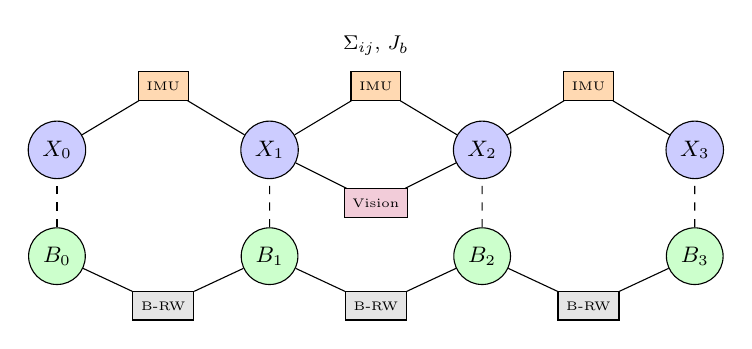
\begin{tikzpicture}[font=\small, scale=0.9, transform shape]
    % Keyframes
    \foreach \i/\x in {0/0, 1/3, 2/6, 3/9} {
      \node[draw, circle, fill=blue!20, minimum size=0.8cm] (X\i) at (\x, 1.5) {$X_\i$};
      \node[draw, circle, fill=green!20, minimum size=0.8cm] (B\i) at (\x, 0)   {$B_\i$};
    }
    % IMU factors
    \foreach \i/\j in {0/1, 1/2, 2/3} {
      \node[draw, rectangle, fill=orange!30, minimum width=0.6cm, minimum height=0.4cm]
        (IMU\i) at ({(\i*3+1.5)}, 2.4) {\tiny IMU};
      \draw (X\i) -- (IMU\i) -- (X\j);
    }
    % Bias random walk factors
    \foreach \i/\j in {0/1, 1/2, 2/3} {
      \node[draw, rectangle, fill=gray!20, minimum width=0.6cm, minimum height=0.4cm]
        (BRW\i) at ({(\i*3+1.5)}, -0.7) {\tiny B-RW};
      \draw (B\i) -- (BRW\i) -- (B\j);
    }
    % Bias to IMU connection
    \foreach \i in {0,1,2,3} {
      \draw[dashed] (B\i) -- (X\i);
    }
    % Vision factors
    \node[draw, rectangle, fill=purple!20, minimum width=0.6cm, minimum height=0.4cm]
      (VIS) at (4.5, 0.75) {\tiny Vision};
    \draw (X1) -- (VIS) -- (X2);
    % Labels
    \node[above=0.1cm of IMU1] {\footnotesize$\Sigma_{ij}$, $J_{b}$};
  \end{tikzpicture}
  \end{center}

  \pause
  \vspace{0.2em}
  \begin{itemize}
    \item IMU factor: $\Sigma_{ij}$, 6개 Jacobian 내장
    \item Bias RW factor: $\Sigma_b = \sigma_{bg}^2\Delta t_{ij}\,I$ 제공
    \item Dashed: 바이어스 $B_i$가 IMU factor 잔차에 영향 (Jacobian을 통해)
    \item Vision factor: 회전/위치 구속 (별도 $\Sigma_{vis}$)
  \end{itemize}
\end{frame}

% ---------- PI-34
\begin{frame}{실습 과제 안내}

  \begin{block}{과제 1: Jacobian 재귀 구현}
    Python 또는 C++ 로 IMU 100 스텝에 대해:
    \begin{enumerate}
      \item $\Delta R_{ij}$, $\Delta v_{ij}$, $\Delta p_{ij}$ 계산
      \item 6개 Bias Jacobian 동시 계산
      \item $\Sigma_{ij}$ 전파
    \end{enumerate}
    제공 파일: \texttt{preintegration\_skeleton.py}
  \end{block}

  \pause
  \begin{block}{과제 2: 선형 보정 검증}
    \begin{enumerate}
      \item $\delta b_g = [0.01, 0, 0]^\top$\;\text{rad/s} 적용
      \item 선형 보정 vs 실제 재적분 결과 비교
      \item 오차가 2차($\propto \|\delta b\|^2$)임을 수치로 확인
    \end{enumerate}
  \end{block}

  \pause
  \begin{exampleblock}{선택 과제: GTSAM 연동}
    GTSAM \texttt{PreintegratedImuMeasurements} 사용하여\\
    factor graph 구성 후 \texttt{iSAM2}로 최적화.\\
    EuRoC V1\_01 데이터셋으로 ATE 측정.
  \end{exampleblock}
\end{frame}

% ---------- PI-35
\begin{frame}{핵심 참고문헌}

  \begin{enumerate}

    \item \textbf{Forster \textit{et al.} (2017)}\\
      ``On-Manifold Preintegration for Real-Time Visual–Inertial Odometry''\\
      \textit{IEEE Transactions on Robotics}, 33(1):1--21.\\
      \textbf{이 강의의 주요 수식 출처} — eq.~(33), (35)--(37), (44)--(46)

    \vspace{0.3em}
    \item \textbf{Lupton \& Sukkarieh (2012)}\\
      ``Visual-Inertial-Aided Navigation for High-Dynamic Motion in Built Environments Without Initial Conditions''\\
      \textit{IEEE TRO}, 28(1):61--76.\\
      (비교 대상: 유클리드 preintegration)

    \vspace{0.3em}
    \item \textbf{Geneva \textit{et al.} (2020)}\\
      ``OpenVINS: A Research Platform for Visual-Inertial Estimation''\\
      \textit{ICRA 2020}.\\
      \url{github.com/rpng/open_vins} (GPLv3)

    \vspace{0.3em}
    \item \textbf{Sola, Deray, Atchuthan (2018)}\\
      ``A micro Lie theory for state estimation in robotics''\\
      \textit{arXiv:1812.01537} — BCH, $J_r$, $J_r^{-1}$ 유도 참고

  \end{enumerate}
\end{frame}

% ========== L5 확장 끝 ==========

\section{6회차: 멀티센서 Update}
% ---------- 1


% ---------- 2
\begin{frame}{지난 시간 한 줄}
  \begin{center}
    \large
    ESKF Predict = 명목 상태(비선형) + 공분산(선형 $\bF_d\bP\bF_d^\top+\bQ_d$).\\
    IMU는 잡음+바이어스가 섞인 신호 — $\bF$로 오차 동역학을 선형화.
  \end{center}
  \vspace{0.5em}
  오늘: \textbf{센서 Update — $\bz$가 들어오면 $\delta\hat\bx$를 어떻게 구하는가}
  \begin{itemize}
    \item GPS (위치, 속도), 휠 인코더 (속도), 카메라 (피처 잔차)
    \item 센서마다 \textbf{H 행렬}이 다름 — 측정을 15D 오차 상태로 이어주는 다리
    \item Mahalanobis 기반 이상값 제거
  \end{itemize}
\end{frame}

% ---------- 3
\begin{frame}{일반 Update 공식}
  ESKF Update step의 구조:
  \begin{align*}
    \bm{r} &= \bz - h(\hatx) \quad\text{(residual: 측정값 $-$ 예측값)} \\
    \bS &= \bH\bP\bH^\top + \bR \\
    \bK &= \bP\bH^\top\bS^{-1} \\
    \delta\hat\bx &= \bK\bm{r} \\
    \bP^+ &= (\bI-\bK\bH)\bP(\bI-\bK\bH)^\top + \bK\bR\bK^\top
  \end{align*}
  \pause
  \vspace{0.2em}
  센서마다 달라지는 것: \textbf{$h(\hatx)$와 $\bH$}. 나머지는 동일.
  \vspace{0.2em}
  \begin{block}{$\bH$의 의미}
    $\bH = \partial h / \partial \dxvec \big|_{\dxvec=0}$ — 15D 오차 상태가 측정 잔차에 얼마나 영향을 미치는가.
  \end{block}
\end{frame}

% ---------- 4
\begin{frame}{GPS 위치 측정 — 가장 단순한 H}
  측정 모델: $\bz_\text{gps} = \bm{p}_\text{true} + \bm{v}_\text{gps}$

  명목 예측: $h(\hatx) = \hatp$

  잔차: $\bm{r} = \bz_\text{gps} - \hatp = (\hatp + \dpvec) - \hatp + \bm{v}_\text{gps} = \dpvec + \bm{v}_\text{gps}$

  \pause
  \vspace{0.3em}
  \textbf{H 행렬} (3×15, 15D 상태 순서 $[\dphivec,\,\dpvec,\,\dvvec,\,\dbgvec,\,\dbavec]$):
  \[
    \bH_\text{pos} = \begin{pmatrix}
      \underbrace{0_{3\times3}}_{\dphivec} &
      \underbrace{\bI_{3\times3}}_{\dpvec} &
      \underbrace{0_{3\times3}}_{\dvvec} &
      \underbrace{0_{3\times3}}_{\dbgvec} &
      \underbrace{0_{3\times3}}_{\dbavec}
    \end{pmatrix}
  \]
  \pause
  \vspace{0.2em}
  \begin{alertblock}{GPS 좌표계}
    GPS는 보통 ECEF 또는 WGS84 (위도/경도/고도). \\
    로컬 ENU로 변환 후 사용하거나, OpenVINS처럼 처음 위치를 원점으로 삼는다.
  \end{alertblock}
\end{frame}

% ---------- 5
\begin{frame}{GPS 속도 측정}
  GPS 수신기의 도플러 기반 속도:
  \[
    \bz_\text{vel} = \bm{v}_\text{true} + \bm{v}_\text{gps\_vel}
  \]
  명목 예측: $h(\hatx) = \hatv$

  \[
    \bH_\text{vel} = \begin{pmatrix}
      0 & 0 & \bI & 0 & 0
    \end{pmatrix} \quad (3\times15)
  \]
  \pause
  \vspace{0.3em}
  GPS는 World frame 속도를 준다. 이것이 ESKF의 $\dvvec$ 블록에 직접 연결됨.
  \vspace{0.3em}
  \begin{block}{GPS 노이즈 모델}
    \begin{itemize}
      \item 위치 정밀도: RTK $\sim$1cm, 단독 $\sim$3m, 도심 $\sim$10m
      \item $\bR_\text{gps}$: 수평보다 수직이 크다 (위성 천정 방향만 있어서)
    \end{itemize}
  \end{block}
\end{frame}

% ---------- 6
\begin{frame}{휠 인코더 — Body frame 속도 측정}
  차동 구동 로봇의 선속도 $v_w$ (Body frame $x$ 방향):
  \[
    \bz_\text{wheel} = \bm{e}_1^\top\,\hatR^\top\,\bm{v}_\text{true} + v_w\text{(noise)}
  \]
  $\bm{e}_1 = (1,0,0)^\top$ (body $x$ 방향 단위 벡터)

  명목 예측: $h(\hatx) = \bm{e}_1^\top\,\hatR^\top\,\hatv$
  \vspace{0.3em}
  \pause
  \textbf{유도} (right perturbation $\bm{R} = \hatR\,\Exp(\dphivec)$, 1차 근사):
  \begin{align*}
    \bm{R}^\top \bm{v} &\approx \hatR^\top(\hatv + \dvvec) + \skewx{\hatR^\top \hatv}\,\dphivec\\
    \Rightarrow\;\; r &= \bm{e}_1^\top\hatR^\top\,\dvvec \;+\; \bm{e}_1^\top\skewx{\hatR^\top\hatv}\,\dphivec \;+\; \text{noise}
  \end{align*}
  여기서 Adjoint 항등식 $\hatR^\top\skewx{\hatv}\hatR = \skewx{\hatR^\top\hatv}$를 사용.

  \textbf{H 행렬} (1×15):
  \[
    \bH_\text{wheel} = \begin{pmatrix}
      \bm{e}_1^\top\skewx{\hatR^\top\hatv} &
      0 &
      \bm{e}_1^\top\hatR^\top &
      0 & 0
    \end{pmatrix}
  \]
  \pause
  \footnotesize
  $\dphivec$ 항이 비자명 — $\skewx{\hatR^\top\hatv}$ 때문에 \emph{속도 측정만으로도 자세 오차 일부를 관측} 가능 (동적 환경에서).
\end{frame}

% ---------- 7
\begin{frame}[shrink=5]{카메라 피처 측정 — MSCKF 원리}
  \textbf{MSCKF} (Multi-State Constraint KF, OpenVINS의 핵심):
  \begin{itemize}
    \item 3D 피처 위치를 직접 상태로 넣지 않음 (EKF-SLAM 대비 저비용)
    \item 대신 여러 카메라 pose에서 같은 피처를 보는 \emph{기하학적 제약} 사용
    \item 피처를 triangulate → 재투영 잔차 → Update
  \end{itemize}
  \pause
  재투영 잔차 (pinhole 카메라):
  \[
    \bm{r}_c = \bz_c - \pi\!\left(\hatR_c^\top(\bm{p}_f - \hat{\bm{p}}_c)\right)
  \]
  $\pi(\bm{p}) = (p_x/p_z,\, p_y/p_z)^\top$: 투영 함수, $\bm{p}_f$: 피처 3D 위치

  \pause
  \begin{block}{H 행렬}
    자세 오차 $\dphivec$와 위치 오차 $\dpvec$ 모두에 의존 (비자명):
    \[
      \bH_c = \bm{J}_\pi \cdot \hatR_c^\top \cdot
              \begin{pmatrix} -\skewx{\bm{p}_f - \hat{\bm{p}}_c} & -\bI \end{pmatrix}
    \]
  \end{block}
\end{frame}

% ---------- 8
\begin{frame}[fragile]{OpenVINS UpdaterMSCKF — H 행렬 구조}
  \texttt{ov\_msckf/src/update/UpdaterMSCKF.cpp}
\begin{lstlisting}[language=C++, basicstyle=\ttfamily\tiny]
// For each camera pose in the window:
// H_x: Jacobian w.r.t. IMU pose error state
// H_f: Jacobian w.r.t. feature position
Eigen::MatrixXd H_xi = Eigen::MatrixXd::Zero(2, 6);  // 2 pixel residual
H_xi.block(0,0,2,3) = dz_dRci * Rcw * skew_x(pf_w - pi_w); // dz/dphi
H_xi.block(0,3,2,3) = dz_dRci * (-Rcw);                     // dz/dp

// Stack all constraints, project out feature uncertainty (nullspace)
// -> reduced H (jacobian only in pose error space)
\end{lstlisting}
  {\footnotesize 출처: \url{github.com/rpng/open_vins} — GPLv3 라이선스}
  \vspace{0.2em}

  \texttt{skew\_x} = $\skewx{\cdot}$, \texttt{Rcw} = $\hatR_c^\top$, \texttt{pf\_w} = $\bm{p}_f$
\end{frame}

% ---------- 9
\begin{frame}{이상값 제거 — Mahalanobis 검정}
  Update 전 잔차가 통계적으로 말이 되는지 확인:
  \[
    d^2 = \bm{r}^\top \bS^{-1} \bm{r} \;\overset{H_0}{\sim}\; \chi^2(\dim\bm{r})
  \]
  \pause
  \begin{itemize}
    \item $d^2 > \chi^2_{0.95}(\dim\bm{r})$ → 이상값으로 판정, Update 건너뜀
    \item GPS multipath, 카메라 dynamic object 등 제거에 필수
  \end{itemize}
  \pause
  \vspace{0.3em}
  \begin{block}{실용 임계값}
    \footnotesize
    \begin{tabular}{lll}
      측정 차원 & $\chi^2_{0.95}$ 임계값 & 사용 예 \\
      \hline
      2 (카메라 픽셀) & 5.99 & OpenVINS 기본값 \\
      3 (GPS 위치) & 7.81 & 위성 수신 불량 \\
      1 (휠 속도) & 3.84 & 슬립 감지 \\
    \end{tabular}
  \end{block}
\end{frame}

% ---------- 10
\begin{frame}{다중 센서 융합 — 실제 순서}
  한 타임스텝에서 여러 센서가 동시에 올 때:
  \vspace{0.3em}
  \begin{enumerate}
    \item IMU → Predict (공분산 부풀음)
    \item GPS 도착 → Mahalanobis 검정 → Update → Inject \& Reset
    \item 카메라 피처 → H matrix → Mahalanobis 검정 → Update → Inject \& Reset
    \item 휠 인코더 → Update (가벼움, 매 step)
  \end{enumerate}
  \pause
  \vspace{0.3em}
  \begin{alertblock}{순차 Update vs 일괄 Update}
    센서들을 독립으로 가정하면 순차(sequential) Update와 일괄 스택(stacked)이 동일.\\
    실제로는 순차가 코드가 간단하고 이상값 제거도 쉽다. OpenVINS도 순차 사용.
  \end{alertblock}
\end{frame}

% ---------- 11
\begin{frame}{레버암(lever arm) — 센서 오프셋 처리}
  GPS 안테나 위치 $\ne$ IMU 위치:
  \[
    \bm{p}_\text{gps} = \bm{p}_\text{IMU} + \bm{R}\,\bm{l}
  \]
  $\bm{l}$: Body frame 레버암 (calibration)
  \vspace{0.3em}
  \pause
  $\bm{l}$를 ESKF 상태에 추가할 수도 있음 (온라인 캘리브레이션).
  \vspace{0.2em}
  잔차 선형화:
  \[
    \bm{r} = \bz_\text{gps} - (\hatp + \hatR\bm{l}) = \dpvec - \skewx{\hatR\bm{l}}\,\dphivec + \ldots
  \]
  \pause
  \begin{block}{H 행렬 수정}
    \[
      \bH_\text{gps+lever} = \begin{pmatrix}
        -\skewx{\hatR\bm{l}} & \bI & 0 & 0 & 0
      \end{pmatrix}
    \]
    자세 오차도 GPS 잔차에 기여함 → 더 많은 정보 (자세 관측 가능)
  \end{block}
\end{frame}

% ---------- 12
\begin{frame}{카메라-IMU 외적 파라미터 (Extrinsic)}
  카메라와 IMU는 다른 위치/방향에 있다:
  \begin{itemize}
    \item $\bm{T}_{BC}$: Body(IMU) frame에서 Camera frame으로의 변환
    \item $\bm{p}_{BC}$: 위치 오프셋, $\bm{R}_{BC}$: 방향 오프셋
  \end{itemize}
  \pause
  \vspace{0.3em}
  캘리브레이션 도구:
  \begin{itemize}
    \item \textbf{Kalibr} (\url{github.com/ethz-asl/kalibr}): IMU + 카메라 외적 캘리브레이션
    \item ESKF 내부에서 $\bm{T}_{BC}$를 상태에 추가 → 온라인 추정 가능
    \item OpenVINS: \texttt{state\_options.do\_calib\_camera\_pose = true}
  \end{itemize}
  \pause
  \vspace{0.2em}
  \begin{block}{실용 팁}
    외적 파라미터 오차가 크면 ESKF가 발산한다.\\
    초기에 Kalibr로 정확히 캘리브레이션 → 이후 온라인 미세조정.
  \end{block}
\end{frame}

% ---------- 13
\begin{frame}{센서 비교 — 관측 가능 상태}
  \begin{center}\footnotesize
  \begin{tabular}{lccccc}
    \toprule
    센서 & $\dpvec$ & $\dvvec$ & $\dphivec$ & $\dbgvec$ & $\dbavec$ \\
    \midrule
    GPS 위치 & \checkmark & & & & \\
    GPS 속도 & & \checkmark & & & \\
    Wheel 속도 & & \checkmark & $\dagger$ & & \\
    카메라 피처 & \checkmark & & \checkmark & & \\
    바로미터 (기압) & $\dagger$ & & & & \\
    자기센서 & & & \checkmark & & \\
    \bottomrule
  \end{tabular}
  \end{center}
  $\dagger$ = 부분적/간접적 관측
  \pause
  \vspace{0.3em}
  \begin{alertblock}{바이어스 관측 가능성}
    바이어스 $\dbgvec, \dbavec$는 센서 하나로는 직접 관측 불가. \\
    \emph{다중} 센서의 교차 정보 + 시간 + 운동 다양성으로만 추정 가능.
  \end{alertblock}
\end{frame}

% ---------- 14
\begin{frame}{이번 회차 핵심 다섯 개}
  \begin{enumerate}
    \item Update 공식은 센서와 무관: $\bm{r}, \bH, \bR, \bK$, Joseph form
    \item 센서마다 $h(\hatx)$와 $\bH$만 달라진다
    \item GPS: $\bH_\text{pos} = [0,\bI,0,0,0]$ — 가장 단순
    \item 휠/카메라: $\dphivec$ 블록이 비자명 → 자세 관측에 기여
    \item Mahalanobis 검정으로 이상값 제거 — 실용 필수
  \end{enumerate}
  \vspace{0.3em}
  \begin{block}{한 줄 요약}
    H 행렬 = ``센서가 15D 오차 공간의 어느 방향을 보고 있는가''.\\
    방향이 다를수록 바이어스 추정에 도움이 된다.
  \end{block}
\end{frame}

% ---------- 15
\begin{frame}{과제 6 (다음 시간 전)}
  \begin{enumerate}
    \item 슬라이드 4의 $\bH_\text{pos}$가 왜 $[\bm{0},\bI,\bm{0},\bm{0},\bm{0}]$인지 잔차 선형화 과정을 직접 유도.
    \item 슬라이드 6의 휠 속도 H 행렬에서 $\skewx{\hatv}$ 항이 등장하는 이유를 수식으로 설명.
          ($\hatR^\top(\hatv+\dvvec) \approx ?$ 에서 시작.)
    \item (선택) OpenVINS \texttt{UpdaterHelper.cpp}의 \texttt{get\_feature\_jacobian\_representation()}
          함수를 읽고, 슬라이드 8의 코드와 대응시켜 설명.
    \item (선택) Mahalanobis 임계값을 100으로 두면 어떤 일이 생기는가? $\chi^2$ 분포 관점에서 해석.
  \end{enumerate}
\end{frame}

% ---------- 16
\begin{frame}{다음 시간 예고 — 7회차: 관측가능성 + 현장 스택}
  \textbf{왜 ESKF가 발산하는가 — 이론과 실전}
  \begin{itemize}
    \item 관측가능성 행렬: 상태가 측정값으로 \emph{결정될 수 있는가}
    \item 기이한 케이스: 자동차 직선 주행 → $\dbgvec$ 비관측
    \item NIS (Normalized Innovation Squared) — 필터 건강도 모니터링
    \item Factor graph로의 이행 (GTSAM, g2o) — smoother와 filter의 차이
    \item 현장 스택 지도: 어떤 프로젝트가 무엇을 쓰는가
  \end{itemize}
  \vspace{0.3em}
  \begin{block}{미리 생각해볼 것}
    로봇이 직선만 달린다면 자이로 z축 바이어스를 추정할 수 있는가?
  \end{block}
\end{frame}

% ---------- 17
\begin{frame}
  \vspace{1.5cm}
  \begin{center}
    {\Huge \textbf{질문 환영}}\\[1em]
    \large H 행렬 하나가 15차원 공간의 어느 방향을 가리키는가
  \end{center}
\end{frame}

% =================================
\section{7회차: 관측가능성 + Factor Graph}
% ---------- 1


% ---------- 2
\begin{frame}{지난 시간 한 줄}
  \begin{center}
    \large
    GPS·휠·카메라는 H 행렬 하나로 15D 오차 공간의 서로 다른 방향을 본다.\\
    Mahalanobis 검정으로 이상값 제거.
  \end{center}
  \vspace{0.5em}
  오늘 (7회차 — ESKF 마무리 + 최적화 세계로의 다리):
  \begin{itemize}
    \item \textbf{Observability}: 어떤 상태가 \emph{원리적으로} 추정 불가인가
    \item \textbf{수치 안정성}: $\bP$ 양정치성 · Joseph form · Cholesky
    \item \textbf{NIS}: 필터 건강도 진단
    \item \textbf{Factor graph + MAP 최적화}: ESKF 너머의 세계 (8/9회차 사전준비)
    \item \textbf{Marginalization}: 슬라이딩 윈도우 VIO의 핵심
    \item \textbf{현장 스택 지도}: 어떤 프로젝트가 무엇을 쓰는가
  \end{itemize}
\end{frame}

% ---------- 3
\begin{frame}{Observability — 정의}
  \begin{block}{Observability (관측 가능성)}
    초기 state $\bx_0$를 \emph{측정 시퀀스}에서 \textbf{유일하게} 복원할 수 있는가?
  \end{block}
  \pause
  \vspace{0.4em}
  \begin{itemize}
    \item Observable: KF가 추정 가능, 분산이 \emph{유한}하게 수렴
    \item Unobservable: 분산이 \emph{영원히} 자란다, 추정 불가능
    \item 어떤 변수가 unobservable인지 \emph{설계 단계}에서 알아야 함
  \end{itemize}
\end{frame}

% ---------- 4
\begin{frame}{선형 시스템의 Observability 행렬}
  \[
    \mathcal{O} = \begin{pmatrix} \bH \\ \bH \bF \\ \bH \bF^2 \\ \vdots \\ \bH \bF^{n-1} \end{pmatrix}
  \]
  \begin{itemize}
    \item $\mathrm{rank}(\mathcal{O}) = n$이면 system은 \textbf{completely observable}
    \item rank $< n$이면 그 차이만큼의 차원이 unobservable
    \item KF의 가장 \emph{이론적} 점검 도구
  \end{itemize}
  \pause
  \vspace{0.3em}
  비선형 시스템 (ESKF): Lie derivative / nonlinear observability 분석.\\
  직관은 동일 — 특정 운동에서 특정 변수가 보이는가.
\end{frame}

% ---------- 5
\begin{frame}{ESKF에서 unobservable인 것들}
  \begin{itemize}
    \item \textbf{절대 위치 (GPS 없을 때)}: dead reckoning만 가능, 분산 무한 성장
    \item \textbf{Yaw (자기계/dual-antenna 없고 정지 시)}: gyro 적분 → drift
    \item \textbf{Accel $z$ bias (정지 자세 유지 시)}: 중력과 구분 불가
    \item \textbf{Gyro $z$ bias (yaw 외부 측정 없을 때)}: yaw drift와 1:1 결합
  \end{itemize}
  \pause
  \vspace{0.3em}
  \begin{block}{교훈}
    Unobservable 변수는 \emph{언젠가는 다른 센서가} 잡아줘야 한다. \\
    그 사이는 분산을 \emph{허용}하고 흘려보내는 것이 정직한 ESKF.
  \end{block}
\end{frame}

% ---------- 6
\begin{frame}{Observability와 Excitation}
  \begin{itemize}
    \item ``원리적 observability''와 ``실제 학습''은 다르다
    \item 자동차가 항상 직진만 하면: yaw가 \emph{사실상} unobservable
    \item 회전을 한 번이라도 하면 yaw bias의 정보가 들어옴
    \item 이걸 \textbf{excitation} (자극)이라고 부름
  \end{itemize}
  \pause
  \vspace{0.3em}
  \begin{block}{practical}
    드론처럼 자세를 자주 바꾸는 시스템은 bias 학습이 빠름. \\
    레일 위 로봇은 영원히 일부 변수를 못 학습.
  \end{block}
\end{frame}

% ---------- 7
\begin{frame}{Mahalanobis distance — 이상치 점검 도구}
  \[
    d^2 = \bm{\nu}^\top \bS^{-1} \bm{\nu}
  \]
  \begin{itemize}
    \item $\bm{\nu} = \bz - h(\hatx)$: residual (innovation)
    \item $\bS = \bH \bP \bH^\top + \bR$: 측정 공간 공분산
    \item $d^2$: \emph{공분산 가중} 거리 — 큰 분산 방향은 ``허용''
  \end{itemize}
  \pause
  \vspace{0.3em}
  \begin{block}{$\chi^2$ 분포}
    측정이 정상이면 $d^2$는 자유도 $n_z$의 $\chi^2$ 분포. \\
    임계값 (95\% 신뢰): $n_z=3$일 때 $d^2 \approx 7.81$.
  \end{block}
\end{frame}

% ---------- 8
\begin{frame}{Mahalanobis 기반 거부}
  매 update step에서:
  \[
    d^2 > d^2_{\text{thresh}} \quad \Rightarrow \quad \text{측정 거부, predict만 진행}
  \]
  \begin{itemize}
    \item GPS multipath, 위성 dropout
    \item 카메라 dynamic object (지나가는 차)
    \item 휠 슬립, 충격
  \end{itemize}
  \pause
  \vspace{0.3em}
  거부하면 그 step은 predict만 진행 → 분산 증가, 그러나 발산 안 함.
  \vspace{0.2em}
  \begin{block}{OpenVINS 기본값}
    카메라 피처 $\chi^2_{0.95}(2) = 5.99$ — \texttt{chi2\_multipler: 1.0}
  \end{block}
\end{frame}

% ---------- 9
\begin{frame}{$\chi^2$ 임계값 잡기}
  \begin{itemize}
    \item 너무 엄격: 정상 측정도 거부 → 정보 손실 → 발산
    \item 너무 느슨: 이상치 통과 → 상태 오염 → 발산
    \item 보통 95\% 또는 99\% 신뢰도
    \item $n_z=3$ at 99\%: $d^2 \approx 11.34$
  \end{itemize}
  \pause
  \vspace{0.3em}
  \begin{block}{practical}
    실험 데이터로 $d^2$ 분포를 그린 후 결정. \\
    제대로 ESKF가 작동하면 $d^2$가 정확히 $\chi^2$를 따름 → consistency 점검 도구.
  \end{block}
\end{frame}

% ---------- 10
\begin{frame}{공분산 $\bP$의 양정치성}
  KF 이론: $\bP$는 항상 \textbf{양 준정치} ($\bx^\top \bP \bx \geq 0$).
  \pause
  \vspace{0.3em}
  실제 코드에서 깨지는 이유:
  \begin{itemize}
    \item Floating point 오차 누적 (특히 $n=15$ 이상)
    \item Update의 짧은 form $(\bI - \bK\bH)\bP$는 음의 고유값 만들 수 있음
    \item $\bR$이 매우 작을 때 수치 오차 증폭
  \end{itemize}
  \pause
  \vspace{0.3em}
  깨지면 → Cholesky 분해 실패 → ESKF 멈춤
  \vspace{0.2em}
  \begin{alertblock}{예방책 우선순위}
    1. \textbf{Joseph form} 사용 \quad 2. 매 step 대칭화 \quad 3. Cholesky 실패 시 shift
  \end{alertblock}
\end{frame}

% ---------- 11
\begin{frame}[fragile]{$\bP$ 대칭화 — 가장 싼 보험}
  매 step 후:
  \[
    \bP \leftarrow \tfrac{1}{2}(\bP + \bP^\top)
  \]
  \begin{itemize}
    \item Floating point 오차로 생긴 비대칭 제거
    \item 비용: 거의 없음
    \item OpenVINS \texttt{StateHelper::EKFUpdate()} 내부에서도 사용:
  \end{itemize}
\begin{lstlisting}[language=C++]
P_new = 0.5 * (P_new + P_new.transpose());
\end{lstlisting}
\end{frame}

% ---------- 12
\begin{frame}{Joseph form 다시 한 번 — 표준}
  Update의 두 가지 form:
  \[
    \bP^+ = (\bI - \bK \bH) \bP \quad (\text{짧은 form — 쓰지 말 것})
  \]
  \[
    \bP^+ = (\bI - \bK\bH)\bP(\bI - \bK\bH)^\top + \bK \bR \bK^\top \quad (\text{Joseph form})
  \]
  \pause
  \vspace{0.3em}
  Short form은 \textbf{최적 게인일 때만} 정확. 수치 오차가 있으면 음의 고유값 생성.
  \vspace{0.2em}
  Joseph form은 \emph{항상} 양정치성을 보장 (대수적으로 $\bP^+$가 PSD임을 증명 가능).
  \vspace{0.2em}
  \begin{alertblock}{규칙: 항상 Joseph form}
    짧은 form을 쓰면 안 되는 이유가 이것. 3회차부터 반복한 이유.
  \end{alertblock}
\end{frame}

% ---------- 13
\begin{frame}{Cholesky 실패 처리 — identity shift}
  공분산이 양정치성을 잃으면:
  \vspace{0.2em}
  \begin{enumerate}
    \item 최솟값 고유값 $\lambda_{\min}$ 계산
    \item $\bP \leftarrow \bP + (-\lambda_{\min} + \epsilon)\bI$ (identity shift)
    \item Cholesky 재시도
  \end{enumerate}
  \pause
  \vspace{0.3em}
  \begin{block}{왜 eigenvalue clamp가 아닌가}
    $\bP$의 eigenvector는 위치·속도·자세 정보가 \emph{혼합}되어 있음. \\
    음의 고유값만 clip하면 다른 차원의 분산도 함께 망가짐. \\
    Identity shift는 \emph{모든} 고유값을 같이 올려 비율 보존.
  \end{block}
\end{frame}

% ---------- 14
\begin{frame}{Time delay와 out-of-order 측정}
  \begin{itemize}
    \item GPS는 처리 지연이 100--200ms 일반적
    \item IMU는 ms 단위, 카메라 exposure + 처리 = 10--50ms
    \item 측정이 ``과거''에 도착하면?
  \end{itemize}
  \pause
  \vspace{0.3em}
  대처:
  \begin{itemize}
    \item \textbf{Buffered KF}: 과거 state를 저장, 측정 도착 시 \emph{재실행}
    \item \textbf{Timestamp 무시}: ``지금 받았다''고 처리 (단순하지만 오차)
    \item \textbf{Retropropagation}: 과거로 되돌려 update 후 현재로 전파
  \end{itemize}
  \pause
  \vspace{0.2em}
  OpenVINS: 카메라 이미지 타임스탬프에 맞춰 IMU propagation을 정확히 맞춤.
\end{frame}

% ---------- 15
\begin{frame}{Multi-rate 센서 처리}
  IMU 100Hz, 카메라 10Hz, GPS 5Hz — 어떻게?
  \pause
  \vspace{0.3em}
  ESKF에서:
  \begin{enumerate}
    \item IMU 도착 시: Predict (명목 + 공분산 전파)
    \item 카메라 도착 시: Update (MSCKF residual)
    \item GPS 도착 시: Update (위치 residual)
  \end{enumerate}
  \pause
  \vspace{0.3em}
  중요: \textbf{predict의 $\Delta t$}는 마지막 IMU로부터의 경과 시간.\\
  매번 정확히 계산해야 process noise $\bQ_d \propto \Delta t$가 맞음.
\end{frame}

% ---------- 16
\begin{frame}{State 초기화 전략}
  \begin{itemize}
    \item Position: GPS 첫 fix를 ENU 원점으로 설정
    \item Velocity: 0 (정지 가정), 분산 크게 ($\sigma_v^2 \sim 1$ m²/s²)
    \item 회전 $\hatR_0$: 가속도계로 roll/pitch, 자기계/GPS로 yaw
    \item Bias: 0, 분산 \emph{크게} (학습되도록 — 초기 정렬 필요)
  \end{itemize}
  \pause
  \vspace{0.3em}
  \begin{block}{practical}
    초기 3--5초는 ``정렬(alignment)'' 구간 — 정지 상태에서 중력 방향 추정.\\
    이 동안 추정값을 \emph{써먹지 말 것}. \\
    NIS가 $\sim n_z$ 근처에서 안정될 때까지 기다림.
  \end{block}
\end{frame}

% ---------- 17
\begin{frame}{NIS — KF 건강도 진단 도구}
  \textbf{Normalized Innovation Squared}:
  \[
    \text{NIS}_k = \bm{r}_k^\top \bS_k^{-1} \bm{r}_k \;\overset{\text{consistent}}{\sim}\; \chi^2(n_z)
  \]
  \begin{itemize}
    \item 평균 $= n_z$이면 KF가 \textbf{일관성 있다}
    \item 평균 $\gg n_z$: 모델 부정확, $\bR$ 또는 $\bQ$ 너무 작음
    \item 평균 $\ll n_z$: $\bR$ 또는 $\bQ$ 너무 큼 (과도한 노이즈 가정)
  \end{itemize}
  \pause
  \vspace{0.3em}
  실험 후 NIS 시계열 plot은 ESKF 튜닝의 \textbf{가장 강력한 도구}.\\
  모든 센서에 대해 별도로 그려라.
\end{frame}

% ---------- 18
\begin{frame}{ESKF 디버깅 — 흔한 함정 7가지}
  \begin{enumerate}
    \item \textbf{Frame 혼동}: World에 있어야 할 양이 Body, 또는 그 반대
    \item \textbf{부호 실수}: gravity 방향, 회전 방향 (우/좌 핸드)
    \item \textbf{시간 동기화}: timestamp 어긋나면 발산
    \item \textbf{공분산 비대칭}: 매 step 대칭화로 예방
    \item \textbf{Bias process noise 너무 작음}: bias 학습 중지
    \item \textbf{측정 분산 $\bR$ 너무 작음}: 노이즈를 진실로 받아들여 발산
    \item \textbf{초기 분산 $\bP_0$ 너무 작음}: 측정이 들어와도 상태 안 움직임
  \end{enumerate}
\end{frame}

% ---------- 19
\begin{frame}{KF 일관성 (Consistency)}
  KF는 ``이 추정의 분산은 $\bP$이다''라고 \emph{주장}한다.\\
  실제 오차 분포가 그 분산과 일치하는가?
  \pause
  \vspace{0.3em}
  \begin{itemize}
    \item \textbf{Optimistic} (overconfident): 실제 오차 $>$ 주장 분산 → 위험
    \item \textbf{Pessimistic}: 실제 오차 $<$ 주장 분산 → 안전하지만 비효율
  \end{itemize}
  \pause
  \vspace{0.3em}
  \begin{block}{측정법}
    Truth 있는 시뮬에서: $\E[(\bx_\text{true}-\hat\bx)(\cdots)^\top]$와 $\bP$ 비교.\\
    실제 시스템: NIS로 간접 점검.
  \end{block}
\end{frame}

% ---------- 20
\begin{frame}{ESKF 너머 — Filter vs Smoother}
  \begin{columns}
    \column{0.48\textwidth}
    \textbf{Filter (ESKF)}
    \begin{itemize}\footnotesize
      \item 온라인, 실시간
      \item 과거 측정 재처리 안 함
      \item 낮은 지연, 낮은 메모리
      \item 로봇 odometry layer에 적합
      \item 정확도 한계: 미래 측정 활용 불가
    \end{itemize}

    \column{0.48\textwidth}
    \textbf{Smoother (Factor Graph)}
    \begin{itemize}\footnotesize
      \item 오프라인 또는 fixed-lag online
      \item 과거 측정도 재처리 (loop closure 등)
      \item 높은 정확도, 높은 메모리
      \item 지도 작성, SLAM, 정밀 캘리브레이션
      \item GTSAM, g2o, Ceres 사용
    \end{itemize}
  \end{columns}
  \pause
  \vspace{0.3em}
  \begin{block}{실제 시스템}
    Filter (ESKF/iEKF) → 빠른 odometry → Factor Graph (smoother) 입력\\
    예: \textbf{FAST-LIO2}(iEKF odometry) + 별도 loop-closure smoother,\\
    \textbf{LIO-SAM}(IMU preintegration + iSAM2 GTSAM smoother)도 동일한 \emph{filter+smoother} 패턴.
  \end{block}
\end{frame}

% ---------- 21
\begin{frame}{Factor Graph 개념 — 10분 소개}
  측정값과 상태를 \textbf{그래프}로 표현:
  \begin{center}
  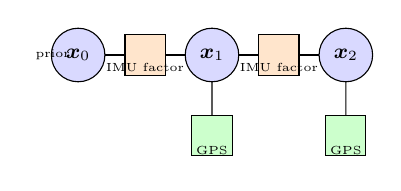
\begin{tikzpicture}[font=\small, scale=0.85, transform shape]
    \node[circle, draw, fill=blue!15, minimum size=0.8cm] (x0) at (0,0) {$\bx_0$};
    \node[circle, draw, fill=blue!15, minimum size=0.8cm] (x1) at (2,0) {$\bx_1$};
    \node[circle, draw, fill=blue!15, minimum size=0.8cm] (x2) at (4,0) {$\bx_2$};
    \node[rectangle, draw, fill=orange!20, minimum size=0.6cm] (f01) at (1,0) {};
    \node[rectangle, draw, fill=orange!20, minimum size=0.6cm] (f12) at (3,0) {};
    \node[rectangle, draw, fill=green!20, minimum size=0.6cm] (z1) at (2,-1.2) {};
    \node[rectangle, draw, fill=green!20, minimum size=0.6cm] (z2) at (4,-1.2) {};
    \node[below] at (1,0) {\tiny IMU factor};
    \node[below] at (3,0) {\tiny IMU factor};
    \node[below=0.05cm] at (2,-1.2) {\tiny GPS};
    \node[below=0.05cm] at (4,-1.2) {\tiny GPS};
    \draw (x0) -- (f01) -- (x1); \draw (x1) -- (f12) -- (x2);
    \draw (x1) -- (z1); \draw (x2) -- (z2);
    \node[left] at (x0) {\tiny prior};
  \end{tikzpicture}
  \end{center}
  \pause
  최적화: 모든 인수의 \textbf{잔차 제곱합 최소화} (MAP = maximum a posteriori)\\
  KF의 단일 step 업데이트 $\equiv$ factor graph의 선형 Gaussian 특수 케이스
\end{frame}

% ---------- 22
\begin{frame}{GTSAM과 IMU Preintegration}
  \textbf{GTSAM} (Georgia Tech Smoothing and Mapping):
  \begin{itemize}
    \item C++ / Python, MIT 라이선스
    \item IMU, GPS, Camera, LiDAR factor 내장
    \item Forster 2017 IMU preintegration 내장 (\texttt{ImuFactor2})
    \item LIO-SAM, VINS-Fusion이 GTSAM 사용
  \end{itemize}
  \pause
  \vspace{0.3em}
  \begin{block}{IMU Preintegration Factor}
    ESKF predict가 매 IMU step 공분산을 전파하듯, \\
    Preintegration factor는 카메라 keyframe 사이 전체 IMU를 하나의 factor로 압축.\\
    바이어스 추정치가 바뀌어도 \emph{선형 보정}으로 재계산 가능.
  \end{block}
\end{frame}

% ---------- 23
\begin{frame}{현장 스택 지도 — 2025}
  \begin{center}\footnotesize
  \begin{tabular}{lll}
    \toprule
    시스템 & 핵심 기술 & 레포 \\
    \midrule
    OpenVINS & ESKF + MSCKF & \texttt{rpng/open\_vins} \\
    FAST-LIO2 & iEKF on SO(3) + ikd-tree & \texttt{hku-mars/FAST\_LIO} \\
    FAST-LIVO2 & iEKF + LiDAR/Visual & \texttt{hku-mars/FAST-LIVO2} \\
    VINS-Mono & Sliding-window factor graph + preint. & \texttt{HKUST-Aerial-Robotics/VINS-Mono} \\
    LIO-SAM & IMU preintegration + GTSAM iSAM2 & \texttt{TixiaoShan/LIO-SAM} \\
    LOAM / LeGO-LOAM & Feature ICP (filter 없음) & \texttt{laboshinl/loam\_velodyne} \\
    Kalibr & Continuous-time batch (Ceres + B-spline) & \texttt{ethz-asl/kalibr} \\
    ROVIO & IEKF on manifold (VIO) & \texttt{ethz-asl/rovio} \\
    GTSAM & Factor graph library & \texttt{borglab/gtsam} \\
    Basalt & IMU preintegration VIO & \texttt{VladyslavUsenko/basalt-headers} \\
    \bottomrule
  \end{tabular}
  \end{center}
  \pause
  \vspace{0.2em}
  \textbf{공통 패턴}: ESKF → 빠른 odometry, Factor graph → 정밀 mapping / loop closure
\end{frame}

% ---------- 24
\begin{frame}[shrink=15]{이 코스 10회를 한 슬라이드로}
  \begin{center}
  \begin{tikzpicture}[font=\scriptsize, scale=0.78, transform shape,
    blk/.style={draw, rounded corners, minimum width=5.4cm, minimum height=0.55cm, align=center}]
    \node[blk, fill=yellow!15] (l0) at (0, 4.5)  {0. 2025 필드 지형도};
    \node[blk, fill=blue!10]   (l1) at (0, 3.6)  {1. Bayes filter, Gaussian};
    \node[blk, fill=blue!10]   (l2) at (0, 2.7)  {2. SO(3) 입문 + Jacobians ($J_r$, BCH)};
    \node[blk, fill=blue!10]   (l3) at (0, 1.8)  {3. 선형 KF};
    \node[blk, fill=orange!15] (l4) at (0, 0.9)  {4. ESKF 핵심 (15D 오차 상태)};
    \node[blk, fill=orange!15] (l5) at (0, 0.0)  {5. IMU + Predict + Preintegration};
    \node[blk, fill=orange!15] (l6) at (0,-0.9)  {6. 멀티센서 Update (H 행렬)};
    \node[blk, fill=red!10]    (l7) at (0,-1.8)  {7. 관측가능성 + Factor Graph + MAP};
    \node[blk, fill=red!10]    (l8) at (0,-2.7)  {8. MSCKF + Visual-Inertial Odometry};
    \node[blk, fill=red!10]    (l9) at (0,-3.6)  {9. LiDAR (FAST-LIO/LIVO)};

    \node[draw, rounded corners, fill=green!15, right=1.4cm of l5, minimum width=4cm, align=center]
      (filt) {\textbf{Filter 스택}\\ OpenVINS\\ FAST-LIO2 / FAST-LIVO2};
    \node[draw, rounded corners, fill=green!15, right=1.4cm of l8, minimum width=4cm, align=center]
      (graph) {\textbf{Graph 스택}\\ GTSAM / iSAM2\\ VINS-Mono / LIO-SAM};
    \foreach \l in {l4, l5, l6} \draw[-Stealth] (\l) -- (filt);
    \foreach \l in {l7, l8, l9} \draw[-Stealth] (\l) -- (graph);
  \end{tikzpicture}
  \end{center}
\end{frame}

% ---------- 25
\begin{frame}{이 코스가 \emph{끝}이 아닌 이유}
  배운 것:
  \begin{itemize}
    \item ESKF — 온라인 filter, IMU + 다중센서, 15D 오차 상태
  \end{itemize}
  \pause
  \vspace{0.3em}
  못 배운 것:
  \begin{itemize}
    \item \textbf{Smoother} (RTS, factor graph, GTSAM) — 사후 정제, 정확도↑
    \item \textbf{SLAM} (loop closure, mapping) — filter 위의 별개 layer
    \item \textbf{Visual-Inertial Odometry 심화} (MSCKF 유도 전 과정, sliding window)
    \item \textbf{Particle filter} — non-Gaussian, 다중 가설
    \item \textbf{Learning-based} (KalmanNet, deep VIO) — 최근 연구
  \end{itemize}
  \pause
  \vspace{0.3em}
  이 코스는 그 모든 것의 \textbf{필수 기초}.
\end{frame}

% ---------- 26
\begin{frame}{이번 회차 핵심 다섯 개}
  \begin{enumerate}
    \item Observability: 어떤 상태는 \emph{원리적으로} 추정 불가 — 설계 단계에서 확인
    \item Joseph form: 항상 사용 — 양정치성 수학적 보장
    \item NIS plot: ESKF 튜닝의 가장 강력한 진단 도구
    \item Filter vs Smoother: ESKF = odometry layer, factor graph = map layer
    \item 실전 스택: OpenVINS / FAST-LIO2 / GTSAM / LIO-SAM 에 이 강의 내용이 모두 들어 있다
  \end{enumerate}
\end{frame}

% ---------- 27
\begin{frame}{학생을 위한 다음 단계 추천}
  \begin{enumerate}
    \item \textbf{Solà 2017} arXiv:1812.01537 — ESKF 표준 교재, 수식 전부 있음
    \item \textbf{Barfoot, \emph{State Estimation for Robotics}} — 이 코스의 정석 교재
    \item \textbf{Forster 2015/2017} (IMU preintegration) — RSS 2015, TRO 2017
    \item OpenVINS 또는 VINS-Mono 코드 전체 읽기 — VIO 입문
    \item GTSAM 튜토리얼 + LIO-SAM 코드 — Factor graph 입문
    \item EuRoC / KITTI 데이터셋에 OpenVINS 돌려보기 — ATE, RPE 평가
  \end{enumerate}
  \pause
  \vspace{0.3em}
  본인의 첫 state estimation 논문은 이 코스 내용 + 추가 6개월이면 가능.
\end{frame}

% ---------- 28
\begin{frame}{과제 7 — 최종}
  \begin{enumerate}
    \item OpenVINS \texttt{Propagator.cpp}를 처음부터 끝까지 읽고,
          \emph{각 코드 블록이 이 강의 어느 수식에 해당하는지} 주석 추가.
    \item 1D ESKF를 직접 구현 (명목 상태 + 오차 상태 분리).\\
          Inject \& Reset 후 오차 분산이 실제로 0이 됨을 확인.
    \item NIS 시계열을 plot하여 튜닝 전후를 비교.
    \item (선택) GTSAM \texttt{examples/ImuFactorExample2} 실행 후 ESKF 결과와 비교.
    \item (선택) FAST-LIO2의 IEKF 코드와 OpenVINS의 ESKF 코드를 비교 분석.
  \end{enumerate}
\end{frame}

% ---------- 29
\begin{frame}{이 코스에서 \emph{기억해야 할} 다섯 줄}
  \begin{enumerate}
    \item \textbf{$p(\bx \mid \bz) \propto p(\bz \mid \bx)\, p(\bx)$} — 모든 KF는 이 줄의 가우시안 특수화
    \item \textbf{$\bK = \bP\bH^\top \bS^{-1}$} — cross-covariance $\times$ 측정 정밀도
    \item \textbf{$\bm{R} = \hatR\,\Exp(\dphivec)$} — ESKF의 핵심: 회전 오차는 $\R^3$에 있다
    \item \textbf{Joseph form 항상} — $\bP^+ = (\bI-\bK\bH)\bP(\bI-\bK\bH)^\top + \bK\bR\bK^\top$
    \item \textbf{NIS로 점검하라} — KF가 자기 분산을 \emph{진짜} 알고 있는지
  \end{enumerate}
\end{frame}

% ---------- 30
\begin{frame}{여러분이 이제 할 수 있는 것}
  \begin{itemize}
    \item OpenVINS \texttt{Propagator.cpp} 한 줄씩 ``왜''를 답함
    \item ESKF가 발산하면 어디서 망가졌는지 \emph{체크리스트}로 진단
    \item 새 센서가 들어오면 H 행렬을 직접 유도하고 구현
    \item Observability, bias, outlier를 \emph{설계 단계}에서 고려
    \item GTSAM factor graph와 ESKF의 관계를 설명
    \item 학위논문에서 ``KF는 검은 상자''라고 안 쓰게 됨
  \end{itemize}
\end{frame}

% ---------- 31
\begin{frame}{Part 1을 마치며 — 한 줄 메시지}
  \begin{center}
    \large
    State estimation은 \emph{기초}이자 \emph{끝}이 없는 분야다.
  \end{center}
  \vspace{0.5em}
  \begin{itemize}
    \item Kalman 1960. 60년 넘게 살아남은 알고리즘
    \item 모든 자율주행, 로봇, 항공기, 위성 안에 들어 있음
    \item 그러나 매 새 센서, 매 새 동역학에서 \emph{새로 풀어야}
    \item ESKF는 그 출발점 — Solà 2017을 읽으면 다음이 보인다
  \end{itemize}
  \pause
  \vspace{0.5em}
  여러분이 이 코스에서 얻은 도구는, 어떤 새 센서, 어떤 새 로봇에서도\\
  ``어디서부터 풀까''를 \emph{스스로 답하게} 해줄 것입니다.
\end{frame}

% ---------- 32 — Part 1 마무리, Part 2로의 다리
\begin{frame}{Part 1 마무리 — 그리고 Part 2로}
  \begin{block}{Part 1: 필터 (0--7회차) 끝}
    여기까지가 \textbf{ESKF 중심의 고전 필터 이론} — Solà 2017 / Barfoot 2017의 영역.\\
    OpenVINS·FAST-LIO2 코드를 줄 단위로 읽을 수 있는 토대를 갖췄다.
  \end{block}
  \vspace{0.4em}
  \pause
  \begin{alertblock}{Part 2: 최적화 + 인접 영역 (이번 회차 후반 + 8/9회차)}
    \begin{itemize}
      \item \textbf{MAP + Marginalization} (이번 회차 후반)
      \item \textbf{MSCKF + Visual-Inertial Odometry} (8회차)
      \item \textbf{LiDAR — FAST-LIO/LIVO} (9회차)
    \end{itemize}
    공통 키워드: Bell\&Cathey 1993의 IEKF$\equiv$Gauss-Newton, sparse $H$, sliding window.
  \end{alertblock}
  \vspace{0.3em}
  \scriptsize 참고문헌(Part 1): Solà 2017 · Barfoot 2017 · Forster 2017 (TRO) · Bell\&Cathey 1993.\\
  레포: OpenVINS (\texttt{rpng/open\_vins}) · FAST-LIO2 (\texttt{hku-mars/FAST\_LIO}) · GTSAM (\texttt{borglab/gtsam}).
\end{frame}

% ========== 7-B: MAP 최적화 + Marginalization (7회차 후반) ==========

% ---------- 7-B 표지 슬라이드
\begin{frame}{\textbf{7-B} — MAP 최적화 \& Marginalization}
  \vspace{0.6em}
  \begin{center}
    {\Large\bfseries 7회차 — Part B}\\[0.4em]
    {\large 필터에서 \emph{최적화}로}
  \end{center}
  \vspace{0.4em}
  \begin{block}{\small 7-A에서 본 것 (방금 마침)}
    Observability · NIS · Joseph form · Factor graph 입문 · Filter+Smoother 패턴
  \end{block}
  \begin{exampleblock}{\small 7-B에서 다룰 것 (이후 ~40 슬라이드)}
    \begin{itemize}
      \item \textbf{MAP 추정} = 비선형 최소제곱 (NLLS)
      \item \textbf{Gauss-Newton / LM} — 그리고 \alert{IEKF $\equiv$ GN의 등치성}
      \item \textbf{Schur complement} — SLAM의 희소 구조 활용
      \item \textbf{Marginalization} — 슬라이딩 윈도우 VIO의 핵심
      \item \textbf{iSAM2} — incremental smoothing, GTSAM의 엔진
    \end{itemize}
  \end{exampleblock}
  \begin{center}\small\itshape\color{gray}
    이 후반부가 8회차(MSCKF) / 9회차(FAST-LIO IEKF)의 토대.
  \end{center}
\end{frame}

%% -----------------------------------------------------------------------
%%  섹션 A — MAP 추정 기초
%% -----------------------------------------------------------------------

% ---------- MAP-1
\begin{frame}{MAP 추정 — 왜 최적화인가?}
  \begin{block}{Bayes 정리에서 출발}
    \[
      p(\bx \mid \bz) \;\propto\; p(\bz \mid \bx)\,p(\bx)
    \]
  \end{block}
  \pause
  \vspace{0.3em}
  \textbf{MAP (Maximum A Posteriori) 추정}:
  \begin{align*}
    \bx^* &= \arg\max_{\bx}\; p(\bx \mid \bz)
           = \arg\min_{\bx}\bigl[-\log p(\bz \mid \bx) - \log p(\bx)\bigr]
  \end{align*}
  \pause
  Gaussian noise 가정 $\Rightarrow$ $-\log p \propto \frac{1}{2}\|r\|_{\Sigma}^2$:
  \[
    \bx^* = \arg\min_{\bx} \sum_i \|r_i(\bx)\|_{\Sigma_i}^2,
    \qquad \|r\|_{\Sigma}^2 \triangleq r^\top \Sigma^{-1} r
  \]
  \pause
  \begin{alertblock}{필터 vs. 최적화}
    \textbf{ESKF}는 이 문제를 \emph{순차적으로 한 번씩} 풀고 버린다.\\
    \textbf{MAP 최적화}는 \emph{전체 윈도우를 한꺼번에} 반복 최적화한다.
  \end{alertblock}
\end{frame}

% ---------- MAP-2
\begin{frame}{비선형 최소제곱 문제로의 변환}
  MAP 목적함수는 \textbf{비선형 최소제곱 (Nonlinear Least Squares, NLLS)}:
  \[
    F(\bx) = \sum_i \|r_i(\bx)\|_{\Sigma_i}^2
           = \sum_i r_i(\bx)^\top \Sigma_i^{-1} r_i(\bx)
  \]
  \pause
  \textbf{Whitening} 변환으로 표준형으로:
  \[
    \tilde{r}_i = \Sigma_i^{-1/2}\,r_i(\bx)
    \quad\Rightarrow\quad
    F(\bx) = \|\tilde{r}(\bx)\|^2 = \sum_i \|\tilde{r}_i(\bx)\|^2
  \]
  \pause
  \begin{block}{SLAM/VIO에서의 residuals $r_i$}
    \begin{itemize}
      \item IMU preintegration residual
      \item 카메라 reprojection residual
      \item Wheel odometry residual
      \item Prior (marginalization으로 생성된 prior factor)
    \end{itemize}
  \end{block}
  \pause
  $\bx$ = 모든 keyframe poses + 속도 + IMU bias + landmarks (특징점).\\
  SLAM에서 변수 수 $\to$ 수천$\sim$수만 차원.
\end{frame}

% ---------- MAP-3
\begin{frame}{Gauss-Newton 알고리즘}
  \textbf{핵심 아이디어}: $r_i(\bx + \delta\bx) \approx r_i(\bx) + J_i\,\delta\bx$ (1차 Taylor)
  \pause
  \begin{align*}
    F(\bx + \delta\bx)
    &\approx \|\tilde{r} + \tilde{J}\,\delta\bx\|^2 \\
    &= \delta\bx^\top \underbrace{(\tilde{J}^\top\tilde{J})}_{H}\,\delta\bx
       + 2\,\underbrace{\tilde{r}^\top\tilde{J}}_{b^\top}\,\delta\bx + \text{const}
  \end{align*}
  \pause
  \begin{block}{Normal Equation}
    \[
      H\,\delta\bx = -b,
      \qquad
      H = \sum_i J_i^\top \Sigma_i^{-1} J_i,
      \quad
      b = \sum_i J_i^\top \Sigma_i^{-1} r_i(\bx)
    \]
    $H$: \textbf{Information matrix} (positive semi-definite)
  \end{block}
  \pause
  \textbf{Update} (manifold 상의 retraction):
  \[
    \bx \;\leftarrow\; \bx \;\boxplus\; (-H^{-1}b)
  \]
  $\boxplus$: SO(3)/SE(3) 위에서는 $\Exp$ map을 통해 적용.\\[0.3em]
  \begin{exampleblock}{수렴}
    초기값이 좋으면 quadratic convergence. IMU로 초기화하면 충분히 좋은 초기값 제공.
  \end{exampleblock}
\end{frame}

% ---------- MAP-3.5  EKF/ESKF ≡ Gauss-Newton (Bell & Cathey 1993)
\begin{frame}[shrink=20]{(E)KF Update $\equiv$ Gauss-Newton 한 스텝}
  \begin{block}{핵심 결과 — Bell \& Cathey (IEEE TAC, 1993)}
    \emph{``The iterated Kalman filter update as a Gauss-Newton method''}\\[0.2em]
    \textbf{IEKF의 한 iteration은 MAP cost에 대한 정확히 한 번의 Gauss-Newton step과 동치이다.}\\
    따라서 \textbf{표준 EKF/ESKF update = Gauss-Newton 1회 iteration}, $\hatx^-$에서 선형화한 결과.
  \end{block}

  \pause
  \vspace{0.3em}
  \textbf{한 스텝 MAP의 cost} (prior $\hatx^-$, $\bP^-$, 측정 $\bz \sim \Norm{\bH\bx}{\bR}$):
  \[
    F(\bx) = \tfrac12\|\bx - \hatx^-\|^2_{(\bP^-)^{-1}} + \tfrac12\|\bz - h(\bx)\|^2_{\bR^{-1}}
  \]
  \pause
  $\hatx^-$ 주변 1차 선형화 후 normal equation을 풀면:
  \[
    \delta\bx^* = (\bP^{-1} + \bH^\top\bR^{-1}\bH)^{-1}\bH^\top\bR^{-1}(\bz - h(\hatx^-))
                = \bK\,(\bz - h(\hatx^-))
  \]
  \pause
  \begin{alertblock}{함의 — 이 코스 전체를 관통하는 한 줄}
    \textbf{ESKF $\subset$ Iterated EKF $\subset$ Gauss-Newton on MAP $\subset$ Factor Graph 최적화}.\\
    필터와 스무더는 \emph{다른 알고리즘이 아니라 같은 cost를 푸는 다른 스케줄}이다.
  \end{alertblock}

  \vspace{0.2em}
  \scriptsize 참고: Bell \& Cathey 1993 · Skoglund, Hendeby, Axehill 2015 (FUSION) · Sibley, Sukhatme, Matthies 2006 (RSS) · Barfoot 2017 §4.2.
\end{frame}

% ---------- MAP-3.6  ESKF는 왜 IEKF로 가야 하는가
\begin{frame}[shrink=20]{ESKF vs.\ Iterated ESKF — \emph{왜 FAST-LIO가 IEKF를 쓰는가}}
  \begin{columns}[T]
    \begin{column}{0.49\textwidth}
      \textbf{표준 ESKF (1-step)}
      \begin{itemize}\footnotesize
        \item Linearize \emph{한 번} at $\hatx^-$
        \item Update 후 종료
        \item 측정 비선형성이 심하면 편향
        \item $h(\hatx^- + \bK\nu) \neq \bz$ 가능
      \end{itemize}
      $\Rightarrow$ Gauss-Newton의 \textbf{1차 iteration}
    \end{column}
    \begin{column}{0.49\textwidth}
      \textbf{Iterated ESKF (IEKF)}
      \begin{itemize}\footnotesize
        \item Re-linearize at 갱신된 $\hatx^{(l)}$
        \item 수렴할 때까지 반복
        \item 비선형 측정에 더 정확
        \item LiDAR point-to-plane에 필수
      \end{itemize}
      $\Rightarrow$ \textbf{전체 Gauss-Newton iteration}
    \end{column}
  \end{columns}

  \pause
  \vspace{0.4em}
  \begin{block}{IEKF iteration $l$ — manifold 형태 (FAST-LIO2 Eq.~18)}
    \footnotesize 표기: $\tilde\bx^{(l)} \triangleq \hatx^{(l)} \boxminus \hatx^-$,\quad
    $r^{(l)} \triangleq \bz - h(\hatx^{(l)})$,\quad
    $\bA^{(l)} \triangleq (\bP^-)^{-1} + \bH^{(l)\top}\bR^{-1}\bH^{(l)}$.
    \[
      \delta\bx^{(l)}
      \;=\; \bigl(\bA^{(l)}\bigr)^{-1}\!
            \bigl(\;\bH^{(l)\top}\bR^{-1}\,r^{(l)}\;-\;(\bP^-)^{-1}\,\tilde\bx^{(l)}\;\bigr)
    \]
    \[
      \hatx^{(l+1)} = \hatx^{(l)} \;\boxplus\; \delta\bx^{(l)}
    \]
    \footnotesize 수렴 조건: $\|\delta\bx^{(l)}\|_\infty < \epsilon$. $l=0$에서 $\tilde\bx^{(0)}=\mathbf{0}$이므로 표준 EKF update와 정확히 일치.
  \end{block}

  \pause
  \begin{exampleblock}{현장 의미}
    FAST-LIO/2/LIVO/LIVO2가 EKF 대신 IEKF를 쓰는 이유 =
    측정 nonlinearity가 큰 LiDAR에서 Gauss-Newton 수렴 정확도가 필요하기 때문.
  \end{exampleblock}
\end{frame}

% ---------- MAP-4
\begin{frame}{Levenberg-Marquardt (LM)}
  \begin{block}{Gauss-Newton의 문제}
    $H$가 singular에 가깝거나 초기값이 나쁠 때 $\delta\bx$가 발산
  \end{block}
  \pause
  \textbf{LM 수정}: 대각 damping 추가
  \[
    H_\lambda\,\delta\bx = -b,
    \qquad
    H_\lambda = H + \lambda\,\mathrm{diag}(H)
  \]
  \pause
  \begin{columns}[T]
    \begin{column}{0.48\textwidth}
      \textbf{$\lambda$ 크면}
      \begin{itemize}
        \item $H_\lambda \approx \lambda\,\mathrm{diag}(H)$
        \item Gradient descent 방향
        \item 느리지만 안정적
        \item 수렴 보장 강함
      \end{itemize}
    \end{column}
    \begin{column}{0.48\textwidth}
      \textbf{$\lambda$ 작으면}
      \begin{itemize}
        \item $H_\lambda \approx H$ (Gauss-Newton)
        \item 빠른 수렴
        \item 초기값 민감
        \item quadratic convergence
      \end{itemize}
    \end{column}
  \end{columns}
  \pause
  \vspace{0.5em}
  \textbf{$\lambda$ 업데이트}: $F$ 감소 $\to$ $\lambda$ 줄임 (GN으로); $F$ 증가 $\to$ $\lambda$ 늘림 (GD로)\\[0.3em]
  \textbf{수렴 기준}: $\|r\|$ 변화 $< \epsilon_1$, $\|\delta\bx\| < \epsilon_2$, $\|b\|_\infty < \epsilon_3$
  \begin{exampleblock}{실용}
    GTSAM, g2o, Ceres Solver에서 기본 nonlinear solver로 채택.
  \end{exampleblock}
\end{frame}

% ---------- MAP-5
\begin{frame}{SLAM의 희소 구조}
  \begin{columns}[T]
    \begin{column}{0.55\textwidth}
      \textbf{Factor graph 구조}:\\
      poses $x_0, x_1, \ldots, x_n$ + landmarks $l_1, \ldots, l_m$\\[0.4em]
      각 factor는 \emph{2$\sim$3개 변수에만 연결}\\
      $\Rightarrow$ Jacobian $J$: \textbf{매우 희소 (sparse)}\\[0.4em]
      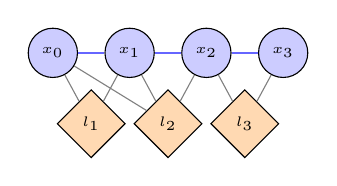
\begin{tikzpicture}[scale=0.75, every node/.style={font=\tiny}]
        % poses
        \foreach \i in {0,1,2,3} {
          \node[circle, draw, fill=blue!20, minimum size=0.55cm] (x\i) at (\i*1.3, 1.2) {$x_\i$};
        }
        % landmarks
        \foreach \j/\xp in {1/0.65, 2/1.95, 3/3.25} {
          \node[diamond, draw, fill=orange!30, minimum size=0.5cm] (l\j) at (\xp, 0) {$l_\j$};
        }
        % odometry edges
        \foreach \i/\ii in {0/1, 1/2, 2/3} {
          \draw[thick, blue!60] (x\i) -- (x\ii);
        }
        % projection edges
        \draw[gray] (x0) -- (l1); \draw[gray] (x1) -- (l1);
        \draw[gray] (x1) -- (l2); \draw[gray] (x2) -- (l2);
        \draw[gray] (x2) -- (l3); \draw[gray] (x3) -- (l3);
        \draw[gray] (x0) -- (l2);
      \end{tikzpicture}
    \end{column}
    \begin{column}{0.42\textwidth}
      $H = J^\top J$: \textbf{sparse symmetric}\\[0.4em]
      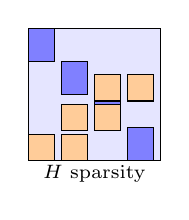
\begin{tikzpicture}[scale=0.42]
        \draw[fill=blue!10] (0,0) rectangle (4,4);
        % diagonal blocks (pose-pose)
        \foreach \i in {0,1,2,3} {
          \draw[fill=blue!50] (\i,3-\i) rectangle (\i+0.8, 4-\i);
        }
        % off-diagonal (pose-landmark)
        \draw[fill=orange!40] (0,0) rectangle (0.8, 0.8);
        \draw[fill=orange!40] (1,0) rectangle (1.8, 0.8);
        \draw[fill=orange!40] (1,0.9) rectangle (1.8, 1.7);
        \draw[fill=orange!40] (2,0.9) rectangle (2.8, 1.7);
        \draw[fill=orange!40] (2,1.8) rectangle (2.8, 2.6);
        \draw[fill=orange!40] (3,1.8) rectangle (3.8, 2.6);
        \node at (2,-0.4) {\scriptsize $H$ sparsity};
      \end{tikzpicture}
    \end{column}
  \end{columns}
  \pause
  \begin{alertblock}{희소성의 중요성}
    Full matrix inverse $O(n^3)$에서 chain topology에서는 sparse solver $O(n)$으로 감소.\\
    100개 keyframe: dense $\to$ \textasciitilde$10^6$ ops, sparse $\to$ \textasciitilde$10^3$ ops (1000배 차이!)
  \end{alertblock}
\end{frame}

% ---------- MAP-6
\begin{frame}{Sparse Cholesky Factorization}
  Symmetric positive definite $H$에 대해:
  \[
    H = L\,L^\top \qquad (L: \text{lower triangular})
  \]
  \pause
  $H\,\delta\bx = -b$ 풀기:
  \begin{enumerate}
    \item $L\,y = -b$ \quad (forward substitution)
    \item $L^\top\,\delta\bx = y$ \quad (backward substitution)
  \end{enumerate}
  \pause
  \begin{block}{Fill-in 문제}
    Cholesky 인수분해 과정에서 0이었던 위치가 nonzero가 되는 현상\\
    $\to$ variable ordering이 fill-in 양에 \emph{결정적}으로 영향
  \end{block}
  \pause
  \begin{columns}[T]
    \begin{column}{0.5\textwidth}
      \textbf{Ordering 알고리즘}
      \begin{itemize}
        \item \textbf{COLAMD}: Column Approximate Minimum Degree
        \item \textbf{AMD}: Approximate Minimum Degree
        \item GTSAM: COLAMD 기본 사용
      \end{itemize}
    \end{column}
    \begin{column}{0.48\textwidth}
      \textbf{구현 라이브러리}
      \begin{itemize}
        \item \texttt{Eigen::SimplicialLLT<>}
        \item \texttt{CHOLMOD} (SuiteSparse)
        \item GTSAM 내장 linear solver
      \end{itemize}
    \end{column}
  \end{columns}
\end{frame}

% ---------- MAP-7
\begin{frame}[shrink=10]{Schur Complement — 블록 구조 활용}
  SLAM의 전형적 $H$ 구조 (poses $p$ + landmarks $l$):
  \[
    H =
    \begin{pmatrix}
      H_{pp} & H_{pl} \\
      H_{lp} & H_{ll}
    \end{pmatrix},
    \qquad
    b =
    \begin{pmatrix}
      b_p \\ b_l
    \end{pmatrix}
  \]
  \pause
  \textbf{핵심 관찰}: $H_{ll}$은 block-diagonal (각 landmark는 독립)\\
  $\Rightarrow$ $H_{ll}^{-1}$은 \emph{각 블록 역행렬의 집합} = 매우 저렴!
  \pause
  \begin{block}{Schur Complement 기법}
    \[
      S \;=\; H_{pp} - H_{pl}\,H_{ll}^{-1}\,H_{lp}
      \quad \text{(reduced system, pose 차원만)}
    \]
    \begin{enumerate}
      \item Reduced system 풀기: $S\,\delta p = -b_p + H_{pl}\,H_{ll}^{-1}\,b_l$
      \item Landmark back-substitution: $\delta l = H_{ll}^{-1}(b_l - H_{lp}\,\delta p)$
    \end{enumerate}
  \end{block}
  \pause
  \begin{exampleblock}{효율}
    1000개 landmarks, 100개 poses: landmark eliminate 후 $100\!\times\!100$ 크기 선형계만 풀면 됨.\\
    VSLAM/SfM (Bundle Adjustment)의 표준 기법.
  \end{exampleblock}
\end{frame}

% ---------- MAP-8
\begin{frame}{iSAM / iSAM2 — Incremental Smoothing and Mapping}
  \begin{block}{SAM의 문제 (Batch)}
    새 factor 추가마다 full re-factorization $\to O(n^3)$:\\
    100 keyframes마다 처음부터 다시 Cholesky 분해 = 실시간 불가
  \end{block}
  \pause
  \textbf{iSAM} (Kaess et al., 2008):
  \begin{itemize}
    \item Cholesky의 rank-1 update 트릭 활용
    \item 주기적 reordering으로 fill-in 관리
    \item $O(n)$ amortized cost
  \end{itemize}
  \pause
  \textbf{iSAM2} (Kaess et al., 2012):
  \begin{itemize}
    \item \textbf{Bayes tree} 자료구조: Cholesky factor를 tree로 인코딩
    \item 새 factor가 추가되면 \emph{영향받는 clique만} 재계산
    \item 실용적으로 단일 factor 추가 = $O(1)$ (sparse graph)
    \item Wildfire 알고리즘: 변경 전파 범위를 tree로 추적
  \end{itemize}
  \pause
  \begin{alertblock}{실제 시스템}
    \textbf{OpenVINS}: EKF 기반, iSAM \emph{미사용}\\
    \textbf{GTSAM 기반 VIO} (e.g., Kimera-VIO): iSAM2 핵심 사용
  \end{alertblock}
\end{frame}

% ---------- MAP-9
\begin{frame}[fragile]{GTSAM 기본 구조}
  \begin{lstlisting}[language=C++]
#include <gtsam/nonlinear/NonlinearFactorGraph.h>
#include <gtsam/nonlinear/Values.h>
#include <gtsam/nonlinear/LevenbergMarquardtOptimizer.h>
#include <gtsam/inference/Symbol.h>
#include <gtsam/geometry/Pose3.h>

NonlinearFactorGraph graph;
Values initialEstimate;

// 첫 번째 pose에 prior 추가 (6-DoF: roll,pitch,yaw,x,y,z)
auto noise = noiseModel::Diagonal::Sigmas(
    (Vector(6) << 0.1, 0.1, 0.1, 0.3, 0.3, 0.3).finished());
graph.addPrior(Symbol('x', 0), Pose3(), noise);
initialEstimate.insert(Symbol('x', 0), Pose3());

// 최적화
LevenbergMarquardtParams params;
params.verbosity = LevenbergMarquardtParams::VALUES;
LevenbergMarquardtOptimizer opt(graph, initialEstimate, params);
Values result = opt.optimize();
  \end{lstlisting}
  \begin{block}{Symbol 네이밍 관례}
    \texttt{'x'}: poses \quad \texttt{'l'}: landmarks \quad
    \texttt{'v'}: velocities \quad \texttt{'b'}: IMU biases
  \end{block}
\end{frame}

% ---------- MAP-10
\begin{frame}[fragile, shrink=15]{GTSAM IMU Factor 예시}
  \begin{lstlisting}[language=C++]
#include <gtsam/navigation/CombinedImuFactor.h>

// 파라미터 설정 (gravity = 9.81, NED or ENU)
auto params = PreintegrationCombinedParams::MakeSharedU(9.81);
params->gyroscopeCovariance     = sigma_gyr * I_3x3;
params->accelerometerCovariance = sigma_acc * I_3x3;
params->biasAccCovariance       = sigma_ba  * I_3x3;

// IMU preintegration (keyframe i -> j 사이)
PreintegratedCombinedMeasurements pim(params, imuBias::ConstantBias());
while (have_imu_data) {
    pim.integrateMeasurement(accel, gyro, dt);
}

// CombinedImuFactor: pose + vel + bias 6개 변수를 동시에 연결
graph.add(CombinedImuFactor(
    X(i), V(i), X(j), V(j), B(i), B(j), pim));
  \end{lstlisting}
  \begin{block}{Combined IMU Factor의 특징}
    \begin{itemize}
      \item IMU preintegration residual (9-dim: position, velocity, rotation)
      \item Bias random walk constraint를 \emph{하나의 factor}로 통합
      \item Bias 공분산 propagation 포함
    \end{itemize}
  \end{block}
\end{frame}

% ---------- MAP-11
\begin{frame}[fragile]{GTSAM — Between Factor \& Pose Graph}
  \begin{lstlisting}[language=C++]
#include <gtsam/slam/BetweenFactor.h>

// 두 pose 사이의 relative transform (odometry, loop closure)
auto odomNoise = noiseModel::Diagonal::Sigmas(
    (Vector(6) << 0.05, 0.05, 0.05, 0.1, 0.1, 0.1).finished());

Pose3 relativePose = pose_i.between(pose_j);  // T_i^{-1} * T_j
graph.add(BetweenFactor<Pose3>(
    Symbol('x', i), Symbol('x', j), relativePose, odomNoise));

// 초기값 설정 및 최적화
for (int k = 0; k <= N; k++)
    initialEstimate.insert(Symbol('x', k), initial_poses[k]);

ISAM2 isam;                   // iSAM2 객체
isam.update(graph, initialEstimate);
Values current = isam.calculateEstimate();
  \end{lstlisting}
  \begin{exampleblock}{iSAM2 incremental update}
    \texttt{isam.update()} 호출마다 Bayes tree를 \emph{증분 업데이트}.\\
    전체 재최적화 없이 실시간 추정값 유지.
  \end{exampleblock}
\end{frame}

% ---------- MAP-12
\begin{frame}[shrink=20]{MAP 최적화 — 수렴 분석}
  \begin{columns}[T]
    \begin{column}{0.5\textwidth}
      \textbf{수렴 보장 조건}
      \begin{itemize}
        \item $H$가 positive definite (관측 가능)
        \item 초기값이 수렴 반경 내
        \item Residual이 smooth (미분 가능)
        \item 충분한 iteration
      \end{itemize}
    \end{column}
    \begin{column}{0.48\textwidth}
      \textbf{실패 상황}
      \begin{itemize}
        \item 잘못된 루프 클로저
        \item 초기값 불량 (global minimum 못 찾음)
        \item Degenerate motion (관측 불가 방향)
        \item 수치 오류 (scale 차이)
      \end{itemize}
    \end{column}
  \end{columns}
  \pause
  \vspace{0.5em}
  \begin{block}{Robustness: Robust Cost Functions}
    Gaussian 대신 \textbf{Huber}, \textbf{Cauchy}, \textbf{GM} 등 robust loss:
    \[
      \rho(r) = \begin{cases}
        \frac{1}{2}r^2 & |r| \le k \quad \text{(quadratic)} \\
        k|r| - \frac{k^2}{2} & |r| > k \quad \text{(linear, Huber)}
      \end{cases}
    \]
    아웃라이어 factor의 영향을 \emph{saturation}으로 제한.
  \end{block}
  \pause
  \begin{exampleblock}{실용}
    GTSAM: \texttt{noiseModel::Robust::Create(HuberModel, baseNoise)}\\
    Ceres: \texttt{new ceres::HuberLoss(k)} 또는 \texttt{CauchyLoss}
  \end{exampleblock}
\end{frame}

% ---------- MAP-13
\begin{frame}{희소 행렬 연산 — 실용 비교}
  \begin{center}
  \begin{tabular}{lccc}
    \toprule
    \textbf{방법} & \textbf{복잡도} & \textbf{메모리} & \textbf{장점} \\
    \midrule
    Dense Cholesky & $O(n^3)$ & $O(n^2)$ & 단순, 작은 시스템 \\
    Sparse Cholesky & $O(n\cdot k^2)$ & $O(n\cdot k)$ & chain graph \\
    Schur complement & $O(m^3 + n\cdot m^2)$ & $O(m^2)$ & VSLAM \\
    iSAM2 & $O(1)$ amortized & $O(n)$ & incremental \\
    \bottomrule
  \end{tabular}
  \end{center}
  ($n$: poses, $m$: landmarks, $k$: bandwidth)
  \pause
  \vspace{0.3em}
  \begin{block}{Variable Elimination Ordering}
    \begin{itemize}
      \item Landmarks를 먼저 eliminate (Schur complement와 동일 효과)
      \item Poses를 나중에 (dense sub-problem)
      \item COLAMD가 자동으로 좋은 ordering 탐색
    \end{itemize}
  \end{block}
\end{frame}

% ---------- MAP-14
\begin{frame}[fragile, shrink=25]{Ceres Solver — 범용 비선형 최소제곱}
  Google의 오픈소스 C++ nonlinear least squares library.
  \begin{lstlisting}[language=C++]
ceres::Problem problem;

// 각 residual block 추가
// ImuCostFunctor: operator() 에서 residual 계산
problem.AddResidualBlock(
    new ceres::AutoDiffCostFunction<ImuCostFunctor, 15, 6, 3, 6, 3, 6>(
        new ImuCostFunctor(preint_meas)),
    new ceres::HuberLoss(1.0),       // robust loss function
    pose_i, vel_i, pose_j, vel_j, bias);

// SO(3) manifold 설정
problem.SetManifold(pose_i, new ceres::EigenQuaternionManifold());

ceres::Solver::Options options;
options.linear_solver_type       = ceres::SPARSE_SCHUR;
options.trust_region_strategy_type = ceres::LEVENBERG_MARQUARDT;
options.num_threads              = 4;
ceres::Solve(options, &problem, &summary);
  \end{lstlisting}
  \begin{exampleblock}{사용 프로젝트}
    COLMAP (SfM), Cartographer (LiDAR SLAM), Open3D, Kalibr (calibration)
  \end{exampleblock}
\end{frame}

% ---------- MAP-15
\begin{frame}[fragile, shrink=25]{g2o — Graph Optimization Library}
  \begin{lstlisting}[language=C++]
#include <g2o/core/sparse_optimizer.h>
#include <g2o/solvers/cholmod/linear_solver_cholmod.h>

g2o::SparseOptimizer optimizer;
// Levenberg-Marquardt + Cholmod solver 조합
auto linearSolver =
    std::make_unique<g2o::LinearSolverCholmod<g2o::BlockSolverX::PoseMatrixType>>();
auto blockSolver  = std::make_unique<g2o::BlockSolverX>(std::move(linearSolver));
auto algorithm    = new g2o::OptimizationAlgorithmLevenberg(std::move(blockSolver));
optimizer.setAlgorithm(algorithm);

// Vertex (pose, landmark) 추가
auto* v = new VertexSE3Expmap();
v->setId(id); v->setEstimate(pose); optimizer.addVertex(v);

// Edge (IMU, camera) 추가
auto* e = new EdgeSE3ProjectXYZ();
e->setVertex(0, optimizer.vertex(pose_id));
e->setVertex(1, optimizer.vertex(landmark_id));
e->setMeasurement(obs); e->setInformation(omega);
optimizer.addEdge(e);

optimizer.optimize(10);   // 10 LM iterations
  \end{lstlisting}
  \begin{exampleblock}{사용 프로젝트}
    ORB-SLAM3, RTAB-Map, LIO-SAM (pose graph part)
  \end{exampleblock}
\end{frame}

% ---------- MAP-16
\begin{frame}{Manifold 최적화 — SO(3)/SE(3) 위에서}
  Euclidean 공간 가정이 깨지는 곳: \textbf{회전}
  \[
    R \in \SOthree \subset \R^{3\times 3},\quad
    \text{but optimizer는 } \R^n \text{에서 동작}
  \]
  \pause
  \begin{block}{Retraction $\boxplus$ and Local Coordinates}
    \[
      R \;\boxplus\; \delta\phi \;=\; R\,\Exp(\delta\phi),
      \qquad \delta\phi \in \R^3
    \]
    Update는 Lie algebra $\sothree$에서, 결과는 $\SOthree$로 map.
  \end{block}
  \pause
  \textbf{구현 방법}:
  \begin{itemize}
    \item GTSAM: \texttt{Rot3}, \texttt{Pose3} 등이 모두 manifold 지원 내장
    \item Ceres: \texttt{EigenQuaternionManifold}, \texttt{SO3Manifold}
    \item g2o: \texttt{VertexSO3Expmap}
  \end{itemize}
  \pause
  \begin{alertblock}{주의}
    Quaternion $q$로 parameterize 시 unit-norm constraint 필요.\\
    Perturbation: $q \leftarrow q \otimes \Exp(\delta\phi/2)$ (half-angle)
  \end{alertblock}
\end{frame}

%% -----------------------------------------------------------------------
%%  섹션 B — Marginalization
%% -----------------------------------------------------------------------

% ---------- MAP-17
\begin{frame}{Marginalization — 왜 필요한가?}
  \begin{block}{Sliding Window Estimator의 딜레마}
    모든 과거 keyframe을 유지 $\to$ 메모리 $O(n^2)$, 계산 $O(n^3)$ 불가피\\
    과거 keyframe을 \emph{단순 삭제} $\to$ 그 frame과 연결된 information 손실
  \end{block}
  \pause
  \textbf{문제 상황}:
  \begin{itemize}
    \item Frame $i$가 landmarks $l_1, l_2, l_3$를 관측 후 윈도우에서 제거
    \item $l_1, l_2, l_3$는 이후에도 사용됨
    \item $i$를 그냥 지우면 $l_1, l_2, l_3$에 가해진 \emph{constraint가 사라짐}
  \end{itemize}
  \pause
  \textbf{해결책: Marginalization}
  \begin{itemize}
    \item 제거할 변수의 information을 \emph{나머지 변수에 prior로 전달}
    \item Gaussian이면 Schur complement로 \textbf{정확히} 수행 가능
    \item \emph{Information 손실 없이} 변수 제거
  \end{itemize}
  \pause
  \begin{alertblock}{핵심 개념}
    Marginalization = 오래된 변수의 information을 ``압축''해서 prior factor로 전환
  \end{alertblock}
\end{frame}

% ---------- MAP-18
\begin{frame}[shrink=20]{Marginalization 이론 — Gaussian Case}
  Joint distribution:
  \[
    p(x_a, x_b) = \Norm{\mu}{\Sigma},
    \qquad
    \Sigma = \begin{pmatrix}\Sigma_{aa} & \Sigma_{ab} \\ \Sigma_{ba} & \Sigma_{bb}\end{pmatrix}
  \]
  \pause
  \textbf{Marginal} ($x_a$ 적분 제거):
  \[
    p(x_b) = \int p(x_a, x_b)\,dx_a = \Norm{\mu_b}{\Sigma_{bb}}
  \]
  \pause
  \textbf{Conditional} ($x_a = \hat{x}_a$ 조건부):
  \begin{align*}
    p(x_b \mid x_a) &= \Norm{\mu_{b|a}}{\Sigma_{b|a}} \\
    \Sigma_{b|a} &= \Sigma_{bb} - \Sigma_{ba}\,\Sigma_{aa}^{-1}\,\Sigma_{ab}
    \quad \leftarrow \text{Schur complement!}
  \end{align*}
  \pause
  \begin{exampleblock}{직관}
    $x_a$를 고정 (또는 제거)하면 $x_b$의 불확실성은 줄어든다 ($\Sigma_{b|a} \le \Sigma_{bb}$).\\
    이 줄어든 불확실성이 바로 $x_a$의 information이 $x_b$로 전달된 결과.
  \end{exampleblock}
\end{frame}

% ---------- MAP-19
\begin{frame}[shrink=20]{Information 행렬에서의 Marginalization}
  \textbf{Information form} (canonical form):
  \[
    p(\bx) \propto \exp\!\left(-\tfrac{1}{2}\bx^\top\Omega\,\bx + \xi^\top\bx\right),
    \quad
    \Omega = \Sigma^{-1},\quad \xi = \Omega\,\mu
  \]
  분할:
  \[
    \Omega = \begin{pmatrix}\Lambda_{aa} & \Lambda_{ab} \\ \Lambda_{ba} & \Lambda_{bb}\end{pmatrix},
    \quad
    \xi = \begin{pmatrix}\xi_a \\ \xi_b\end{pmatrix}
  \]
  \pause
  \begin{block}{$x_a$를 marginalize out한 결과 — $x_b$의 prior}
    \begin{align*}
      \Omega_{b}^{\mathrm{marg}} &= \Lambda_{bb} - \Lambda_{ba}\,\Lambda_{aa}^{-1}\,\Lambda_{ab} \\
      \xi_{b}^{\mathrm{marg}}    &= \xi_b - \Lambda_{ba}\,\Lambda_{aa}^{-1}\,\xi_a
    \end{align*}
  \end{block}
  \pause
  \begin{alertblock}{핵심: Information form의 장점}
    \textbf{Marginalization} (information form) = \textbf{Schur complement} (covariance form)\\
    Information 행렬에서 marginalization이 더 직접적으로 표현됨!
  \end{alertblock}
  \pause
  \begin{exampleblock}{결과 해석}
    $\Omega_b^{\mathrm{marg}}$: $x_a$가 $x_b$에 준 정보를 \emph{모두 흡수}한 새 prior\\
    Prior factor 형태: $\|x_b - x_b^*\|_{\Omega_b^{\mathrm{marg}}}^2$
  \end{exampleblock}
\end{frame}

% ---------- MAP-20
\begin{frame}{Sliding Window Marginalization — 단계별 과정}
  \begin{enumerate}
    \setlength\itemsep{0.4em}
    \item \textbf{Identify}: 제거할 변수 $x_a$ 결정\\
      (oldest keyframe + 그와만 연결된 landmarks)
    \pause
    \item \textbf{Linearize}: $x_a$와 연결된 \emph{모든 factor} 선형화\\
      $r_i(x_a, x_b) \approx r_i^0 + J_{ia}\,\delta x_a + J_{ib}\,\delta x_b$\\
      \textbf{중요}: 현재 linearization point에서 고정
    \pause
    \item \textbf{Schur Complement}: $x_a$ eliminate\\
      $\Omega_b^{\mathrm{marg}}, \xi_b^{\mathrm{marg}}$ 계산
    \pause
    \item \textbf{Prior Factor 생성}: 결과를 나머지 변수 $x_b$에 대한\\
      Gaussian prior로 추가: $\|x_b - x_b^*\|_{\Omega_b^{\mathrm{marg}}}^2$
    \pause
    \item \textbf{Remove}: $x_a$와 연결된 원래 factor들을 삭제,\\
      $x_a$ 변수 제거 (prior factor만 남김)
  \end{enumerate}
  \pause
  \begin{alertblock}{Linearization Point 고정 문제}
    Step 2에서 고정된 linearization point가 이후 추정값과 멀어지면\\
    prior가 \emph{inconsistent}해짐 $\to$ FEJ (First Estimates Jacobian)로 대응 (8회차)
  \end{alertblock}
\end{frame}

% ---------- MAP-21
\begin{frame}{Prior Factor as Marginalization Result}
  \textbf{Marginalization 결과 = 비선형 prior factor의 선형 근사}
  \[
    f_{\mathrm{prior}}(x_b) = \left\|x_b \ominus x_b^*\right\|_{\Omega^{\mathrm{marg}}}^2
  \]
  ($\ominus$: manifold에서의 차이, $= \Log(x_b^{*-1} \cdot x_b)$ on SE(3))
  \pause
  \begin{columns}[T]
    \begin{column}{0.55\textwidth}
      \textbf{특성}
      \begin{itemize}
        \item 단 한 번의 선형화 근사
        \item 이후 $x_b$가 변해도 linearization point 고정
        \item Dense block: marginalize된 $x_a$가 연결했던 모든 $x_b$들 간에 correlation 생성
        \item Prior의 $\Omega^{\mathrm{marg}}$는 일반적으로 dense (full rank)
      \end{itemize}
    \end{column}
    \begin{column}{0.42\textwidth}
      \textbf{문제점}
      \begin{itemize}
        \item 시간이 지나 $x_b$가 많이 변하면 prior inconsistent
        \item Spurious information 축적 가능
        \item 주기적 marginalization으로 관리 필요
      \end{itemize}
    \end{column}
  \end{columns}
  \pause
  \begin{exampleblock}{구현 예}
    OKVIS (Leutenegger et al., 2015): marginalization prior를 명시적으로 관리\\
    Kimera-VIO: GTSAM의 \texttt{LinearContainerFactor}로 구현
  \end{exampleblock}
\end{frame}

% ---------- MAP-22
\begin{frame}{Marginalization — 수식 유도 (전체)}
  $x_a$와 연결된 factor들로부터 local linear system:
  \[
    \begin{pmatrix}\Lambda_{aa} & \Lambda_{ab} \\ \Lambda_{ba} & \Lambda_{bb}\end{pmatrix}
    \begin{pmatrix}\delta x_a \\ \delta x_b\end{pmatrix}
    = -\begin{pmatrix}\xi_a \\ \xi_b\end{pmatrix}
  \]
  \pause
  Block elimination ($x_a$ 제거):
  \begin{align*}
    \Lambda_{aa}\,\delta x_a &= -\xi_a - \Lambda_{ab}\,\delta x_b \\
    \delta x_a &= -\Lambda_{aa}^{-1}(\xi_a + \Lambda_{ab}\,\delta x_b)
  \end{align*}
  \pause
  $\delta x_b$ 방정식에 대입:
  \begin{align*}
    \underbrace{(\Lambda_{bb} - \Lambda_{ba}\Lambda_{aa}^{-1}\Lambda_{ab})}_{\Omega^{\mathrm{marg}}}\,\delta x_b
    &= -\underbrace{(\xi_b - \Lambda_{ba}\Lambda_{aa}^{-1}\xi_a)}_{\xi^{\mathrm{marg}}}
  \end{align*}
  \pause
  \begin{block}{결과}
    \[
      \Omega^{\mathrm{marg}} = \Lambda_{bb} - \Lambda_{ba}\Lambda_{aa}^{-1}\Lambda_{ab}, \qquad
      \xi^{\mathrm{marg}} = \xi_b - \Lambda_{ba}\Lambda_{aa}^{-1}\xi_a
    \]
    이것이 $x_b$에 대한 \textbf{새로운 prior의 information matrix와 information vector}.
  \end{block}
\end{frame}

% ---------- MAP-23
\begin{frame}{Fixed-lag Smoother vs. Full Bundle Adjustment}
  \begin{columns}[T]
    \begin{column}{0.48\textwidth}
      \begin{block}{Full Bundle Adjustment (BA)}
        \begin{itemize}
          \item \emph{모든} keyframe을 한꺼번에 최적화
          \item 가장 정확 (global consistency)
          \item 메모리: $O(n^2)$
          \item 계산: $O(n^3)$ per iteration
          \item 오프라인 처리에 적합
          \item COLMAP, OpenSfM
        \end{itemize}
      \end{block}
    \end{column}
    \begin{column}{0.48\textwidth}
      \begin{block}{Fixed-lag Smoother}
        \begin{itemize}
          \item 최근 $W$개 keyframe만 윈도우 유지
          \item 메모리: $O(W^2)$ (bounded)
          \item 계산: $O(W^3)$ per step
          \item 오래된 것 $\to$ marginalization
          \item 실시간 가능
          \item VINS-Mono ($W=10$), OKVIS
        \end{itemize}
      \end{block}
    \end{column}
  \end{columns}
  \pause
  \vspace{0.4em}
  \begin{center}
  \begin{tabular}{lccc}
    \toprule
    \textbf{시스템} & \textbf{방법} & \textbf{Window} & \textbf{특징} \\
    \midrule
    VINS-Mono & Fixed-lag & 10 KF & Marginalization \\
    OKVIS & Fixed-lag & 5 KF & ISAM2-style \\
    Kimera-VIO & iSAM2 & adaptive & Bayes tree \\
    ORB-SLAM3 & Full BA & local+global & 두 단계 \\
    COLMAP & Full BA & all & 오프라인 SfM \\
    \bottomrule
  \end{tabular}
  \end{center}
\end{frame}

% ---------- MAP-24
\begin{frame}{Filtering vs. Smoothing 재고찰}
  \begin{columns}[T]
    \begin{column}{0.48\textwidth}
      \begin{block}{ESKF (Filtering)}
        \begin{itemize}
          \item 순차적 처리, $O(1)$ per step
          \item Propagation + Update
          \item 선형화: \emph{현재 추정값}에서 1회
          \item 메모리: $O(n^2)$ ($n$: state 차원, 고정)
          \item 과거 추정값 수정 \emph{불가}
          \item OpenVINS, FAST-LIO, LOAM
        \end{itemize}
      \end{block}
    \end{column}
    \begin{column}{0.48\textwidth}
      \begin{block}{MAP Smoothing}
        \begin{itemize}
          \item 윈도우 전체 반복 최적화
          \item Gauss-Newton / LM
          \item 선형화: \emph{매 iteration마다} 갱신
          \item 메모리: window 크기에 비례
          \item 윈도우 내 과거 추정값 \emph{수정 가능}
          \item GTSAM/iSAM2, g2o-based
        \end{itemize}
      \end{block}
    \end{column}
  \end{columns}
  \pause
  \vspace{0.5em}
  \begin{alertblock}{이론적 동등성 vs. 실제 차이}
    Gaussian, linear 가정 하에서는 \textbf{이론적으로 동등} (EKF = MAP with window=1)\\
    실제: 비선형성, 여러 번의 재선형화, loop closure 처리에서 큰 차이 발생
  \end{alertblock}
  \pause
  \begin{exampleblock}{언제 무엇을?}
    \textbf{ESKF}: 실시간, 단순 센서 퓨전, 계산 제약 환경\\
    \textbf{MAP}: 정밀도 중요, 루프 클로저 필요, 오프라인 가능
  \end{exampleblock}
\end{frame}

% ---------- MAP-25
\begin{frame}{Marginalization vs. 단순 삭제 — 시뮬레이션 비교}
  \begin{columns}[T]
    \begin{column}{0.5\textwidth}
      \textbf{단순 삭제 (Drop)}
      \begin{tikzpicture}[scale=0.9, font=\small]
        \node[circle, draw, fill=red!20] (x0) at (0,1.5) {$x_0$};
        \node[circle, draw, fill=blue!20] (x1) at (1.5,1.5) {$x_1$};
        \node[circle, draw, fill=blue!20] (x2) at (3,1.5) {$x_2$};
        \node[diamond, draw, fill=orange!20] (l1) at (0.75,0) {$l_1$};
        \draw[blue, thick] (x0)--(x1); \draw[blue, thick] (x1)--(x2);
        \draw[gray] (x0)--(l1); \draw[gray] (x1)--(l1);
        \draw[red, very thick, dashed] (0.6,1.0) circle (0.5);
        \node[red, font=\tiny] at (0.6,0.3) {삭제};
      \end{tikzpicture}
      \begin{itemize}
        \item $x_0 \to l_1$ constraint \textbf{소실}
        \item $l_1$의 불확실성 증가
        \item Inconsistent estimator
      \end{itemize}
    \end{column}
    \begin{column}{0.5\textwidth}
      \textbf{Marginalization}
      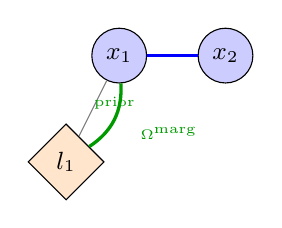
\begin{tikzpicture}[scale=0.9, font=\small]
        \node[circle, draw, fill=blue!20] (x1) at (1.5,1.5) {$x_1$};
        \node[circle, draw, fill=blue!20] (x2) at (3,1.5) {$x_2$};
        \node[diamond, draw, fill=orange!20] (l1) at (0.75,0) {$l_1$};
        \draw[blue, thick] (x1)--(x2);
        \draw[gray] (x1)--(l1);
        \draw[green!60!black, very thick] (x1) to[bend left=30]
          node[above, font=\tiny] {prior} (l1);
        \node[green!60!black, font=\tiny] at (2.2,0.4) {$\Omega^{\text{marg}}$};
      \end{tikzpicture}
      \begin{itemize}
        \item $x_0$의 정보가 prior로 전달
        \item $l_1$, $x_1$ 간 correlation 유지
        \item \textbf{Consistent} estimator
      \end{itemize}
    \end{column}
  \end{columns}
  \pause
  \begin{block}{수치 예시}
    $x_0$ 삭제 시 $l_1$의 covariance: Drop $\to 2\sigma^2$, Marginalize $\to 0.5\sigma^2$
  \end{block}
\end{frame}

% ---------- MAP-26
\begin{frame}[shrink=10]{Marginalization — 연결 변수 선택 전략}
  \begin{block}{어떤 변수를 marginalize할 것인가?}
    \begin{enumerate}
      \item \textbf{Oldest keyframe}: 시간 순서로 가장 오래된 frame
      \item \textbf{Redundant keyframe}: 가장 최근 frame과 motion이 작은 frame
      \item \textbf{Associated features}: marginalize되는 frame에만 보이는 landmarks
    \end{enumerate}
  \end{block}
  \pause
  \textbf{중요한 규칙}: marginalize할 변수는 \emph{남아 있는 변수들과의 연결이 최소}여야 함
  \begin{itemize}
    \item 연결이 많으면 $\Omega^{\mathrm{marg}}$가 dense해져 prior 처리가 무거워짐
    \item Sparsification: 약한 연결은 무시 (Drop edge with small information)
  \end{itemize}
  \pause
  \begin{columns}[T]
    \begin{column}{0.55\textwidth}
      \textbf{VINS-Mono 전략}
      \begin{itemize}
        \item 충분한 시차(parallax) 없으면 second-newest frame marginalize
        \item 충분한 시차 있으면 oldest frame marginalize
        \item 목적: 윈도우 내 정보량 최대화
      \end{itemize}
    \end{column}
    \begin{column}{0.42\textwidth}
      \textbf{OKVIS 전략}
      \begin{itemize}
        \item 5 keyframes + 5 temporal frames
        \item Keyframe 제거 시 marginalization
        \item Temporal frame 제거 시 drop
      \end{itemize}
    \end{column}
  \end{columns}
\end{frame}

% ---------- MAP-27
\begin{frame}{FEJ (First Estimate Jacobian) — Marginalization과의 연결}
  \textbf{문제}: Marginalization에서 linearization point를 한번 고정
  \begin{itemize}
    \item Prior factor의 Jacobian은 $\hat{x}_b^{(\mathrm{fixed})}$에서 계산됨
    \item 이후 optimization에서 $x_b$의 estimate가 바뀌어도 Jacobian 고정
    \item Prior factor와 새 factor의 \emph{linearization point가 불일치} $\to$ inconsistency
  \end{itemize}
  \pause
  \begin{block}{FEJ (First Estimate Jacobian) 해결책}
    모든 factor의 Jacobian을 \emph{처음 linearize된 시점의 값으로 고정}\\
    $\Rightarrow$ marginalization의 linearization point와 일관성 유지
  \end{block}
  \pause
  \[
    J_i^{\mathrm{FEJ}} = \frac{\partial r_i}{\partial x}\Bigg|_{x = \hat{x}^{(1\mathrm{st})}}
    \quad \text{(이후 업데이트에서도 동일 값 사용)}
  \]
  \pause
  \begin{exampleblock}{적용 시스템}
    MSCKF + FEJ: OpenVINS에서 관측가능성 보존에 활용\\
    VINS-Fusion: marginalization과 FEJ 결합\\
    이론: Huang et al., ``Observability-based Rules for Designing Consistent EKF SLAM'' (2010)
  \end{exampleblock}
\end{frame}

% ---------- MAP-28
\begin{frame}[fragile, shrink=15]{GTSAM — Marginalization 구현}
  \begin{lstlisting}[language=C++]
#include <gtsam/nonlinear/ISAM2.h>
#include <gtsam/nonlinear/LinearContainerFactor.h>

ISAM2 isam2;
NonlinearFactorGraph newFactors;
Values newValues;

// ... factor/value 추가 후 ...
isam2.update(newFactors, newValues);

// 변수 marginalize (oldest keyframe 제거)
FastList<Key> marginalizeKeys;
marginalizeKeys.push_back(Symbol('x', oldest_id));
marginalizeKeys.push_back(Symbol('v', oldest_id));
marginalizeKeys.push_back(Symbol('b', oldest_id));

// Marginal factor를 graph에 남김
ISAM2Result result = isam2.update();
// ISAM2는 내부적으로 Bayes tree를 통해 marginalization 처리
auto marginalFactor = isam2.marginalizeLeaves(marginalizeKeys);
  \end{lstlisting}
  \begin{block}{GTSAM의 marginalization 방식}
    \texttt{marginalizeLeaves()}: Bayes tree의 leaf 변수를 제거하고\\
    해당 정보를 parent clique의 factor로 변환
  \end{block}
\end{frame}

% ---------- MAP-29
\begin{frame}{Bounded Memory Optimization — 요약}
  \begin{center}
  \begin{tikzpicture}[
    font=\small,
    node distance=1.2cm,
    box/.style={rectangle, draw, rounded corners, fill=blue!10, minimum width=3cm, minimum height=0.7cm, align=center},
    arrow/.style={->, thick, >=Stealth}
  ]
    \node[box] (new)  {새 IMU/Camera 측정};
    \node[box, below of=new] (add) {Factor graph에 추가};
    \node[box, below of=add] (opt) {LM 최적화\\(Window 내)};
    \node[box, below of=opt] (check) {Window 크기 초과?};
    \node[box, below right=0.7cm and 1.5cm of check, fill=orange!20]
          (marg) {Marginalization\\(oldest KF 제거)};
    \node[box, below of=check, fill=green!10] (out) {추정값 출력};

    \draw[arrow] (new)  -- (add);
    \draw[arrow] (add)  -- (opt);
    \draw[arrow] (opt)  -- (check);
    \draw[arrow] (check) -- node[right]{\tiny Yes} (marg);
    \draw[arrow] (check) -- node[left]{\tiny No}  (out);
    \draw[arrow] (marg) |- (out);
  \end{tikzpicture}
  \end{center}
  \pause
  \begin{block}{메모리/계산 복잡도 보장}
    Window $W$로 고정 $\to$ 메모리 $O(W)$, 계산 $O(W^3)$ (bounded)\\
    실시간 로봇에서 수백 Hz IMU, 30 Hz camera 처리 가능
  \end{block}
\end{frame}

% ---------- MAP-30
\begin{frame}{실제 VIO 시스템에서의 Marginalization}
  \begin{columns}[T]
    \begin{column}{0.48\textwidth}
      \begin{block}{VINS-Mono (Hong Kong UST, 2018)}
        \begin{itemize}
          \item Window: 10 keyframes
          \item Marginalization: Schur complement 직접 구현
          \item Feature: co-visibility graph로 keyframe 선택
          \item 논문: Qin et al., TRO 2018
        \end{itemize}
      \end{block}
    \end{column}
    \begin{column}{0.48\textwidth}
      \begin{block}{Kimera-VIO (MIT SPARK, 2020)}
        \begin{itemize}
          \item iSAM2 기반 (GTSAM)
          \item Bayes tree로 자동 marginalization
          \item Mesh 생성 + semantic 연동
          \item 논문: Rosinol et al., ICRA 2020
        \end{itemize}
      \end{block}
    \end{column}
  \end{columns}
  \pause
  \vspace{0.4em}
  \begin{columns}[T]
    \begin{column}{0.48\textwidth}
      \begin{block}{OKVIS (ETH Zurich, 2015)}
        \begin{itemize}
          \item Sliding window, Ceres Solver
          \item Marginalization prior 명시적 관리
          \item 4-cam stereo+IMU 지원
          \item 논문: Leutenegger et al., IJRR 2015
        \end{itemize}
      \end{block}
    \end{column}
    \begin{column}{0.48\textwidth}
      \begin{block}{OpenVINS (UofDelaware, 2020)}
        \begin{itemize}
          \item MSCKF 기반 EKF (marginalization 없음)
          \item SLAM features로 부분 최적화
          \item 오픈소스, ROS2 지원
          \item 논문: Geneva et al., ICRA 2020
        \end{itemize}
      \end{block}
    \end{column}
  \end{columns}
\end{frame}

% ---------- MAP-31
\begin{frame}{Loop Closure — MAP 최적화와의 결합}
  \begin{block}{Loop Closure란?}
    이전에 방문한 장소를 다시 인식하여 누적 drift를 보정하는 것
  \end{block}
  \pause
  \textbf{처리 방법} (MAP smoothing 관점):
  \begin{enumerate}
    \item Place recognition: bag-of-words (DBoW2, VLAD) 또는 학습 기반
    \item Relative pose 추정: PnP, essential matrix
    \item Loop closure factor 추가: $\|x_i \ominus x_j - \Delta T_{ij}\|_{\Sigma}^2$
    \item Full BA 또는 pose graph optimization으로 global consistency
  \end{enumerate}
  \pause
  \begin{alertblock}{Filtering에서의 어려움}
    ESKF는 과거 추정값을 \emph{수정할 수 없어} loop closure 처리가 매우 어려움\\
    $\to$ 별도 pose graph layer 필요 (SLAM 프레임워크의 ``back-end'')
  \end{alertblock}
  \pause
  \begin{exampleblock}{ORB-SLAM3의 접근}
    Front-end: feature tracking (EKF-like)\\
    Back-end: local BA (g2o) + loop detection\\
    Loop closure: essential graph optimization (pose graph)
  \end{exampleblock}
\end{frame}

% ---------- MAP-32
\begin{frame}[shrink=10]{Pose Graph Optimization — 경량화 BA}
  \textbf{아이디어}: feature를 모두 명시적으로 유지하지 않고, \emph{poses 간 relative constraint만} 유지
  \[
    F_{\mathrm{pg}} = \sum_{(i,j)\in\mathcal{E}}
      \left\|\Log\!\left(T_j^{-1}\,T_{ij}\,T_i\right)\right\|_{\Sigma_{ij}}^2
  \]
  \pause
  \begin{columns}[T]
    \begin{column}{0.5\textwidth}
      \textbf{장점}
      \begin{itemize}
        \item 변수: poses만 ($n$개 $\times$ 6-DoF)
        \item 빠른 optimization
        \item Loop closure에 최적
        \item 전체 trajectory 일관성
      \end{itemize}
    \end{column}
    \begin{column}{0.48\textwidth}
      \textbf{단점 / 한계}
      \begin{itemize}
        \item Feature position 정보 손실
        \item Relative pose uncertainty 누적
        \item Full BA보다 덜 정확
        \item Front-end에 의존
      \end{itemize}
    \end{column}
  \end{columns}
  \pause
  \vspace{0.3em}
  \begin{block}{Edge 종류}
    \begin{itemize}
      \item \textbf{Odometry edge}: 연속 pose 간 (IMU preintegration, wheel)
      \item \textbf{Loop closure edge}: 재방문 감지 시
      \item \textbf{GPS factor}: absolute position constraint
    \end{itemize}
  \end{block}
  \pause
  \begin{exampleblock}{구현}
    g2o: \texttt{EdgeSE3} + \texttt{VertexSE3}\\
    GTSAM: \texttt{BetweenFactor<Pose3>} + \texttt{NonlinearFactorGraph}
  \end{exampleblock}
\end{frame}

% ---------- MAP-33
\begin{frame}{MAP 최적화 — 계산 비용 실전 분석}
  \begin{center}
  \begin{tabular}{lcccc}
    \toprule
    \textbf{알고리즘} & \textbf{변수 수} & \textbf{Factor 수} & \textbf{시간/step} & \textbf{비고} \\
    \midrule
    Pose graph (g2o) & $n$ poses & $\sim 2n$ & $<$5ms & loop closure \\
    Local BA (GTSAM) & $n$+$m$ & $\sim 5n$ & 10--30ms & VIO window \\
    Full BA (Ceres) & 모두 & 모두 & $>$1s & 오프라인 \\
    iSAM2 increment & +1 KF & +few & $<$5ms & 실시간 \\
    \bottomrule
  \end{tabular}
  \end{center}
  ($n$: poses, $m$: landmarks, 10--100 KF 기준 측정값)
  \pause
  \vspace{0.3em}
  \begin{block}{실시간 VIO 타이밍 (예: Intel i7, 30Hz camera)}
    \begin{itemize}
      \item Feature tracking: 2--5ms
      \item IMU preintegration: $<$1ms
      \item MAP optimization (window=10): 10--20ms
      \item Total budget at 30Hz: 33ms
    \end{itemize}
  \end{block}
\end{frame}

% ---------- MAP-34
\begin{frame}{Gaussian Belief Propagation — Factor Graph와 Message Passing}
  \textbf{대안적 관점}: MAP optimization을 \emph{message passing}으로 해석
  \begin{block}{Sum-Product Algorithm on Factor Graph}
    \[
      \mu_{f_i \to x_j}(x_j) = \int \prod_{k \neq j} \mu_{x_k \to f_i}(x_k) \cdot f_i(x_j, \{x_k\})\, dx_k
    \]
    Gaussian일 때: message = Gaussian, 곱셈 = information matrix 덧셈
  \end{block}
  \pause
  \begin{itemize}
    \item Tree 구조: exact inference, $O(n)$
    \item Loopy graph: iterative (belief propagation, convergence 미보장)
    \item iSAM2의 Bayes tree = message passing의 효율적 구현
  \end{itemize}
  \pause
  \begin{exampleblock}{연결}
    \textbf{Kalman Filter}: factor graph에서 chain topology의 message passing\\
    \textbf{RTS Smoother}: forward (KF) + backward (message) pass\\
    \textbf{MAP optimization}: iterative linearization + sparse linear solve
  \end{exampleblock}
\end{frame}

% ---------- MAP-35
\begin{frame}[fragile, shrink=30]{전체 VIO 파이프라인 — 코드 구조 (GTSAM 기반)}
  \begin{lstlisting}[language=C++, basicstyle=\ttfamily\tiny]
class VIOEstimator {
    ISAM2 isam2_;
    NonlinearFactorGraph newFactors_;
    Values newValues_;
    int current_kf_id_ = 0;

    void addImuFactor(int i, int j, PreintegratedCombinedMeasurements& pim) {
        newFactors_.add(CombinedImuFactor(X(i),V(i),X(j),V(j),B(i),B(j), pim));
    }
    void addCameraFactor(int kf_id, int lm_id, Vector2 obs, Cal3_S2 K) {
        newFactors_.add(GenericProjectionFactor<Pose3,Point3,Cal3_S2>(
            obs, noiseModel::Isotropic::Sigma(2, 1.5),
            X(kf_id), L(lm_id), boost::make_shared<Cal3_S2>(K)));
    }
    void marginalize(int oldest_id) {
        FastList<Key> toMarg = {X(oldest_id), V(oldest_id), B(oldest_id)};
        isam2_.marginalizeLeaves(toMarg);
    }
    Values update() {
        isam2_.update(newFactors_, newValues_);
        newFactors_.resize(0); newValues_.clear();
        return isam2_.calculateEstimate();
    }
};
  \end{lstlisting}
\end{frame}

% ---------- MAP-36
\begin{frame}[shrink=20]{Observability와 MAP 최적화의 관계}
  \textbf{7회차 앞부분에서 배운 Observability를 MAP 관점에서 재해석}
  \pause
  \begin{block}{Observability $\leftrightarrow$ Information Matrix}
    \[
      \text{Observable} \iff H = \sum_i J_i^\top \Sigma_i^{-1} J_i \;\text{가 positive definite}
    \]
    Null space of $H$ = Unobservable directions\\
    $H$의 eigenvalue $\approx 0$ $\to$ 해당 방향 추정 불가 (발산)
  \end{block}
  \pause
  \textbf{SLAM의 대표적 unobservable 방향}:
  \begin{itemize}
    \item \textbf{절대 위치}: 세계 좌표계 원점 (no GPS $\to$ unobservable)
    \item \textbf{절대 heading} (monocular+IMU): roll, pitch = observable, yaw = unobservable
    \item \textbf{절대 scale} (monocular): feature depth unobservable
  \end{itemize}
  \pause
  \begin{alertblock}{MAP 최적화에서의 처리}
    Prior factor를 추가하여 null space를 fix:
    \begin{itemize}
      \item Position prior: $x_0$에 고정 prior
      \item Heading prior: 초기 orientation prior
      \item Scale: stereo 또는 depth sensor로 관측 가능하게
    \end{itemize}
  \end{alertblock}
\end{frame}

% ---------- MAP-37
\begin{frame}[shrink=10]{MAP 최적화 — 수치 안정성 기법}
  \begin{columns}[T]
    \begin{column}{0.5\textwidth}
      \textbf{변수 정규화 (Normalization)}
      \begin{itemize}
        \item Position: meter 단위 유지
        \item Rotation: unit quaternion enforce
        \item Landmark: 관측 가능한 범위로 초기화
        \item 센서 noise를 같은 스케일로 설정
      \end{itemize}
      \vspace{0.3em}
      \textbf{Gauge Fixing}
      \begin{itemize}
        \item 첫 pose를 world frame에 fix
        \item 또는 prior factor로 soft fix
        \item 절대 좌표계 고정 $\to$ $H$ positive definite
      \end{itemize}
    \end{column}
    \begin{column}{0.48\textwidth}
      \textbf{Huber Loss (이상값 억제)}
      \[
        \rho_H(r) = \begin{cases}
          \frac{1}{2}r^2 & |r| \le k \\
          k|r| - \frac{k^2}{2} & |r| > k
        \end{cases}
      \]
      \textbf{Covariance Conditioning}
      \begin{itemize}
        \item $H$에 작은 대각 damping: $H + \epsilon I$
        \item Condition number 모니터링
        \item 수치 Cholesky 실패 시 fallback
      \end{itemize}
      \vspace{0.3em}
      \textbf{Iteration 제한}
      \begin{itemize}
        \item Max iterations 설정
        \item Convergence 미달 시 경고
      \end{itemize}
    \end{column}
  \end{columns}
\end{frame}

% ---------- MAP-38
\begin{frame}{LiDAR SLAM에서의 MAP 최적화}
  \textbf{LiDAR 특화 MAP 최적화 기법}:
  \pause
  \begin{block}{Scan Matching = 비선형 최소제곱}
    \[
      T^* = \arg\min_{T \in \SEthree} \sum_{i} \|n_i^\top(T\,p_i - q_i)\|^2
    \]
    $p_i$: source point, $q_i$: target point/plane, $n_i$: surface normal
  \end{block}
  \pause
  \textbf{대표 알고리즘}:
  \begin{itemize}
    \item \textbf{ICP} (Iterative Closest Point): point-to-point, GN으로 수렴
    \item \textbf{NDT} (Normal Distribution Transform): voxel 단위 Gaussian
    \item \textbf{LOAM/LeGO-LOAM}: edge+surface feature matching, g2o
    \item \textbf{LIO-SAM}: IMU tight-coupled, GTSAM factor graph
    \item \textbf{FAST-LIO2}: iEKF (iterative EKF) + ikd-tree
  \end{itemize}
  \pause
  \begin{exampleblock}{LIO-SAM의 factor graph 구성}
    IMU preintegration factor + scan matching between factor + GPS factor + loop closure factor\\
    GTSAM 기반, fixed-lag smoothing 적용
  \end{exampleblock}
\end{frame}

% ---------- MAP-39
\begin{frame}[shrink=20]{딥러닝과 MAP 최적화의 결합}
  \textbf{학습 기반 front-end + MAP 기반 back-end} 구조:
  \pause
  \begin{columns}[T]
    \begin{column}{0.55\textwidth}
      \textbf{Front-end (학습 기반)}
      \begin{itemize}
        \item Feature detection: SuperPoint, ALIKE
        \item Feature matching: SuperGlue, LightGlue
        \item Depth 추정: monodepth2, DPT
        \item Place recognition: NetVLAD, DBoW3
        \item Pose regression: PoseNet (참고용)
      \end{itemize}
    \end{column}
    \begin{column}{0.42\textwidth}
      \textbf{Back-end (MAP 최적화)}
      \begin{itemize}
        \item GTSAM / g2o / Ceres
        \item Factor graph 구조 동일
        \item 학습 기반 noise model
        \item Uncertainty 정량화 필요
      \end{itemize}
    \end{column}
  \end{columns}
  \pause
  \vspace{0.4em}
  \begin{block}{최신 트렌드}
    \textbf{End-to-end differentiable SLAM}: factor graph 내 학습 파라미터\\
    DROID-SLAM: dense bundle adjustment + DNN, GRU로 update step 학습\\
    DeepFactors: learned depth uncertainty를 factor graph에 직접 통합
  \end{block}
  \pause
  \begin{alertblock}{한계}
    학습 모델의 불확실성 추정이 부정확하면 MAP 최적화도 망가짐\\
    $\Rightarrow$ calibration된 uncertainty (conformal prediction 등) 필요
  \end{alertblock}
\end{frame}

% ---------- MAP-40
\begin{frame}[shrink=20]{요약: MAP 최적화 체계}
  \begin{enumerate}
    \setlength\itemsep{0.5em}
    \item \textbf{MAP = 비선형 최소제곱}\\
      $\bx^* = \arg\min \sum_i \|r_i(\bx)\|_{\Sigma_i}^2$,
      Gaussian noise $\to$ negative log-likelihood
    \pause
    \item \textbf{Gauss-Newton / Levenberg-Marquardt}\\
      Normal equation $H\,\delta\bx = -b$, LM damping으로 안정화\\
      manifold 위에서 retraction $\boxplus$ 사용
    \pause
    \item \textbf{SLAM의 희소성 활용}\\
      Sparse Cholesky, Schur complement, variable ordering (COLAMD)\\
      dense $O(n^3) \to$ sparse $O(n)$ (chain graph)
    \pause
    \item \textbf{iSAM2: incremental 인수분해}\\
      Bayes tree + Wildfire: 영향받는 변수만 재계산\\
      단일 factor 추가 $\approx O(1)$ 실용적 복잡도
    \pause
    \item \textbf{Marginalization: Schur complement로 오래된 변수 제거}\\
      information 보존하며 변수 제거, prior factor로 전달\\
      Fixed-lag smoother = bounded memory MAP optimization
  \end{enumerate}
  \pause
  \vspace{0.3em}
  \begin{alertblock}{다음 회차 (L8) 예고}
    이 MAP 최적화가 \textbf{MSCKF}와 어떻게 다른가? FEJ, Nullspace projection,\\
    관측가능성 보존 — EKF와 MAP의 이론적 통합 관점
  \end{alertblock}
\end{frame}

%% ---- 보너스 프레임 (optional, 시간 여유 시) ----

% ---------- MAP-A1
\begin{frame}{부록: Information Filter vs. Kalman Filter}
  \textbf{Kalman Filter (Covariance form)}:
  \begin{align*}
    \text{Predict: }&\bP^- = \bF\bP\bF^\top + \bQ \\
    \text{Update: }&\bK = \bP^-\bH^\top(\bH\bP^-\bH^\top+\bR)^{-1},\quad
    \bP^+ = (\bI - \bK\bH)\bP^-
  \end{align*}
  \pause
  \textbf{Information Filter} ($\Omega = \bP^{-1}$, $\xi = \Omega\,\hat{\bx}$):
  \begin{align*}
    \text{Predict: }&\Omega^- = (\bF\Omega^{-1}\bF^\top + \bQ)^{-1} \\
    \text{Update: }&\Omega^+ = \Omega^- + \bH^\top\bR^{-1}\bH,\quad
    \xi^+ = \xi^- + \bH^\top\bR^{-1}\bz
  \end{align*}
  \pause
  \begin{block}{비교}
    \begin{itemize}
      \item KF update: $O(n^2 m)$ ($m$: 측정 차원)
      \item IF update: $O(n^2 m)$ 비슷하나 \emph{measurement fusion이 더 간단}
      \item IF predict: $O(n^3)$ (역행렬 필요) — 단점
      \item 분산 fusion, multi-robot에서 IF가 유리 (information 덧셈)
    \end{itemize}
  \end{block}
\end{frame}

% ---------- MAP-A2
\begin{frame}{부록: Bundle Adjustment — SfM에서의 MAP}
  \textbf{Classical Bundle Adjustment (Triggs et al., 1999)}:
  \[
    \min_{\{T_i\}, \{X_j\}} \sum_{i,j} \rho\!\left(\left\|x_{ij} - \pi(T_i, X_j)\right\|_{\Sigma}^2\right)
  \]
  $T_i$: camera poses, $X_j$: 3D landmark, $\pi(\cdot)$: projection, $\rho$: robust loss
  \pause
  \begin{block}{구조}
    \begin{itemize}
      \item 변수: $n \times 6$-DoF poses + $m \times 3$-DoF landmarks
      \item Jacobian: $2 \times (6+3)$ per reprojection
      \item $H$ 구조: ``arrow'' (poses) + ``diagonal'' (landmarks)
      \item Schur complement로 landmark 먼저 eliminate
    \end{itemize}
  \end{block}
  \pause
  \begin{exampleblock}{현대 SfM 파이프라인}
    COLMAP: SuperPoint feature + Ceres BA\\
    OpenMVG: 고도로 최적화된 sparse BA\\
    NeRF/3DGS: differentiable rendering + BA 결합
  \end{exampleblock}
\end{frame}

% ---------- MAP-A3
\begin{frame}{부록: 참고문헌 및 추천 자료}
  \begin{columns}[T]
    \begin{column}{0.5\textwidth}
      \textbf{교재/리뷰}
      \begin{itemize}
        \item Grisetti et al., ``A Tutorial on Graph-Based SLAM,'' IEEE IS 2010
        \item Dellaert \& Kaess, ``Factor Graphs for Robot Perception,'' FnTR 2017
        \item Barfoot, ``State Estimation for Robotics,'' Cambridge 2017
        \item Nocedal \& Wright, ``Numerical Optimization,'' Springer 2006
      \end{itemize}
    \end{column}
    \begin{column}{0.48\textwidth}
      \textbf{핵심 논문}
      \begin{itemize}
        \item Kaess et al., ``iSAM2,'' IJRR 2012
        \item Leutenegger et al., ``OKVIS,'' IJRR 2015
        \item Qin et al., ``VINS-Mono,'' TRO 2018
        \item Triggs et al., ``Bundle Adjustment — A Modern Synthesis,'' 1999
        \item Rosinol et al., ``Kimera-VIO,'' ICRA 2020
      \end{itemize}
    \end{column}
  \end{columns}
  \pause
  \vspace{0.4em}
  \textbf{오픈소스 코드}
  \begin{itemize}
    \item \texttt{https://gtsam.org} — GTSAM (Georgia Tech)
    \item \texttt{https://github.com/RainerKuemmerle/g2o} — g2o
    \item \texttt{http://ceres-solver.org} — Ceres (Google)
    \item \texttt{https://github.com/HKUST-Aerial-Robotics/VINS-Mono}
    \item \texttt{https://github.com/MIT-SPARK/Kimera-VIO}
  \end{itemize}
\end{frame}

% ============================================================
%  Lecture 8 — MSCKF + Visual-Inertial Odometry
%  Part of: Modern Robot State Estimation Lecture (8-lecture series)
%  Author: generated for gsk course, 2026-04-30
% ============================================================

\section{8회차: MSCKF + Visual-Inertial Odometry}

% ---------- 8회차 — 지난 시간 한 줄
\begin{frame}{지난 시간 한 줄 — 7회차에서 8회차로}
  \begin{center}\large
    \textbf{필터 = Gauss-Newton의 1회 iter},\\
    \textbf{IEKF = Gauss-Newton 전체 iter},\\
    \textbf{MAP = 모든 keyframe을 동시에 최적화}.
  \end{center}
  \vspace{0.3em}
  \begin{block}{\small 7회차에서 본 것}
    \begin{itemize}
      \item Observability · NIS · Joseph form
      \item MAP $\equiv$ NLLS · Gauss-Newton/LM · Schur complement
      \item \alert{Bell \& Cathey 1993: ESKF $\subset$ IEKF $\equiv$ GN on MAP $\subset$ Factor Graph}
      \item Marginalization, iSAM2
    \end{itemize}
  \end{block}
  \pause
  \begin{exampleblock}{오늘 (8회차) — 한 단계 위로}
    그 위에 \textbf{Sliding Window}를 얹은 \alert{MSCKF (Multi-State Constraint KF)}.\\
    카메라 pose를 ``복제(stochastic cloning)''하고, feature uncertainty를 \\
    \textbf{null-space projection}으로 algebraic하게 제거 → OpenVINS의 본체.
  \end{exampleblock}
\end{frame}


% ---------- L8-1
\begin{frame}{8회차 로드맵 — MSCKF \& Visual-Inertial Odometry}
  \begin{columns}[T]
    \column{0.48\textwidth}
      \begin{block}{오늘 다룰 내용}
        \begin{enumerate}
          \item \textbf{파트 1}: MSCKF 구조 및 기초
          \item \textbf{파트 2}: Null-space projection
          \item \textbf{파트 3}: Feature triangulation
          \item \textbf{파트 4}: FEJ (First Estimate Jacobian)
          \item \textbf{파트 5}: IMU-카메라 캘리브레이션
          \item \textbf{파트 6}: OpenVINS 전체 파이프라인
        \end{enumerate}
      \end{block}
    \column{0.48\textwidth}
      \begin{alertblock}{핵심 질문}
        \begin{itemize}
          \item Feature를 state에 넣지 않고도 VIO가 가능한가?
          \item Feature depth ambiguity를 어떻게 처리하는가?
          \item EKF의 consistency 문제를 어떻게 해결하는가?
          \item IMU와 카메라를 정확히 맞추려면?
        \end{itemize}
      \end{alertblock}
      \begin{exampleblock}{Key Reference}
        Mourikis \& Roumeliotis, ICRA 2007\\
        Geneva et al.\ (OpenVINS), ICRA 2020
      \end{exampleblock}
  \end{columns}
\end{frame}

% ---------- L8-2
\begin{frame}{MSCKF 등장 배경 — EKF-SLAM의 한계}
  \begin{columns}[T]
    \column{0.50\textwidth}
      \begin{block}{EKF-SLAM의 문제}
        \begin{itemize}
          \item Feature를 state에 포함
          \item $N$ features $\Rightarrow$ state 차원 $+3N$
          \item Covariance update: $O(N^2)$
          \item 실시간 운영 한계 ($N \gtrsim 100$에서 느림)
        \end{itemize}
      \end{block}
      \begin{block}{EKF-SLAM state 구조}
        \begin{align*}
          \bx_{\text{SLAM}} &= \bigl[\bx_{\text{IMU}}^\top,\;
                              {}^G\bm{p}_{f_1}^\top,\;\ldots,\;
                              {}^G\bm{p}_{f_N}^\top\bigr]^\top
        \end{align*}
        $\Rightarrow$ $15 + 3N$ 차원, $N$이 증가하면 폭발적 증가
      \end{block}
    \column{0.46\textwidth}
      \begin{exampleblock}{MSCKF의 해법 (Mourikis \& Roumeliotis, ICRA 2007)}
        \begin{itemize}
          \item Feature를 state에 \textbf{넣지 않음}
          \item 대신: 여러 카메라 \textbf{pose에서 같은 feature}를 보는 기하학적 제약 사용
          \item State: IMU + 카메라 pose 슬라이딩 윈도우
          \item Complexity: $O(N_{\text{feat}})$ per update step
        \end{itemize}
      \end{exampleblock}
      \begin{alertblock}{핵심 통찰}
        Feature의 절대 위치가 아닌\\
        \textbf{다중 뷰 기하학적 제약}만 사용
      \end{alertblock}
  \end{columns}
\end{frame}

% ---------- L8-3
\begin{frame}[shrink=10]{MSCKF 상태 벡터 구조}
  \begin{block}{IMU State (L4 ESKF와 동일)}
    \begin{align*}
      \bx_{\text{IMU}} &= \bigl[{}^I_G\bm{R},\; {}^G\bm{p}_I,\; {}^G\bm{v}_I,\; \bm{b}_g,\; \bm{b}_a\bigr]
      \;\in\; \SOthree \times \R^{12}, \quad \text{error-state: } \R^{15}
    \end{align*}
  \end{block}
  \begin{block}{Camera Clone State (슬라이딩 윈도우)}
    \begin{align*}
      \bx_{C_i} &= \bigl[{}^{C_i}_G\bm{R},\; {}^G\bm{p}_{C_i}\bigr]
      \;\in\; \SOthree \times \R^3, \quad \text{error-state: } \R^6
    \end{align*}
    $i = 1, \ldots, N$: 최근 $N$개의 카메라 keyframe poses
  \end{block}
  \begin{block}{Full State Vector}
    \begin{align*}
      \bx &= \bigl[\bx_{\text{IMU}}^\top,\; \bx_{C_1}^\top,\; \ldots,\; \bx_{C_N}^\top\bigr]^\top
      \;\in\; \R^{15 + 6N}
    \end{align*}
  \end{block}
  \begin{columns}[T]
    \column{0.48\textwidth}
      \begin{exampleblock}{OpenVINS 기본값}
        \begin{itemize}
          \item Sliding window 크기 $N = 10\text{--}20$
          \item $N=15$: state dim $= 15 + 90 = 105$
        \end{itemize}
      \end{exampleblock}
    \column{0.48\textwidth}
      \begin{alertblock}{주의}
        Camera pose가 추가될수록 state 증가\\
        $\Rightarrow$ Marginalization으로 관리 필요
      \end{alertblock}
  \end{columns}
\end{frame}

% ---------- L8-4
\begin{frame}[shrink=10]{Stochastic Cloning — 카메라 Pose 추가}
  \begin{block}{아이디어}
    IMU propagation 후 새 카메라 frame에 도달할 때,\\
    현재 IMU state에서 카메라 pose를 \textbf{복제(clone)}하여 state에 추가
  \end{block}
  \begin{block}{Covariance Augmentation}
    Clone 전 state $\bx$, covariance $P$에서:
    \begin{align*}
      \bx^{\text{aug}} &= \begin{pmatrix}\bx \\ \bx_{C_k}\end{pmatrix},
      \qquad
      P^{\text{aug}} = \begin{pmatrix}
        P_{xx} & P_{xx} J_c^\top \\
        J_c P_{xx} & J_c P_{xx} J_c^\top
      \end{pmatrix}
    \end{align*}
    $J_c \in \R^{6\times 15}$: camera pose $\bx_{C_k}$의 IMU state $\bx_{\text{IMU}}$에 대한 Jacobian
  \end{block}
  \begin{columns}[T]
    \column{0.50\textwidth}
      \begin{exampleblock}{왜 ``Stochastic'' Cloning?}
        \begin{itemize}
          \item 단순 복사가 아님
          \item 기존 state와의 \textbf{상관관계 구조}를 정확히 반영
          \item $P_{xx}J_c^\top$: 새 clone과 기존 state 간 cross-correlation
        \end{itemize}
      \end{exampleblock}
    \column{0.46\textwidth}
      \begin{alertblock}{잘못 구현 시}
        Cross-correlation 무시 $\Rightarrow$\\
        Information 손실, inconsistency\\
        (covariance 과소 추정)
      \end{alertblock}
  \end{columns}
\end{frame}

% ---------- L8-5
\begin{frame}[shrink=10]{Cloning Jacobian $J_c$ 계산}
  \begin{block}{Camera Pose와 IMU State의 관계}
    Extrinsic calibration: ${}^C_I T = ({}^C_I R,\; {}^I\bm{p}_C)$
    \begin{align*}
      {}^{C_k}_G R &= {}^C_I R \cdot {}^I_G R \\
      {}^G\bm{p}_{C_k} &= {}^G\bm{p}_I + {}^I_G R^\top \cdot {}^I\bm{p}_C
    \end{align*}
  \end{block}
  \begin{block}{Error-state Jacobian}
    Rotation 부분 ($\dphivec_{C_k}$ w.r.t.\ $\dphivec_I$):
    \begin{align*}
      \dphivec_{C_k} &\approx {}^C_I R \cdot \dphivec_I
      \quad\Rightarrow\quad J_{c,R} = {}^C_I R \in \R^{3\times 3}
    \end{align*}
    Position 부분 ($\dpvec_{C_k}$ w.r.t.\ $\dphivec_I,\, \dpvec_I$):
    \begin{align*}
      \dpvec_{C_k} &\approx \dpvec_I - \skewx{{}^I_G R^\top\, {}^I\bm{p}_C}\,\dphivec_I
      \quad\Rightarrow\quad J_{c,p} = \bigl[-\skewx{\hatR^\top\,{}^I\bm{p}_C},\; \bI_3\bigr]
    \end{align*}
  \end{block}
  \begin{exampleblock}{Full $J_c \in \R^{6\times 15}$}
    \begin{align*}
      J_c = \begin{pmatrix}
        {}^C_I R & 0_{3\times 3} & 0_{3\times 3} & 0_{3\times 6} \\
        -\skewx{\hatR^\top {}^I\bm{p}_C} & \bI_3 & 0_{3\times 3} & 0_{3\times 6}
      \end{pmatrix}
    \end{align*}
    (rotation 3, position 3, velocity 3, biases 6 = 15 columns)
  \end{exampleblock}
\end{frame}

% ---------- L8-6
\begin{frame}{Sliding Window 관리 — MSCKF State 진화}
  \begin{block}{MSCKF 한 사이클}
    \begin{enumerate}
      \item \textbf{IMU Propagation}: $\hatR, \hatp, \hatv, \hatbg, \hatba$ 및 $P$ 전파
      \item \textbf{Stochastic Cloning}: 현재 카메라 pose를 state에 복제
      \item \textbf{Feature Tracking}: KLT optical flow, feature tracks 업데이트
      \item \textbf{MSCKF Update}: track이 끝난 feature로 update (null-space proj.)
      \item \textbf{SLAM Update}: 오래 살아남은 feature (선택적)
      \item \textbf{Marginalization}: 오래된 camera clone 제거
    \end{enumerate}
  \end{block}
  \begin{columns}[T]
    \column{0.48\textwidth}
      \begin{exampleblock}{Keyframe vs.\ All Frames}
        \begin{itemize}
          \item 모든 이미지마다 clone할 필요 없음
          \item 충분한 baseline 기준으로 keyframe 선택
          \item OpenVINS: 카메라 fps에 맞춰 clone
        \end{itemize}
      \end{exampleblock}
    \column{0.48\textwidth}
      \begin{alertblock}{Marginalization 방법}
        \begin{itemize}
          \item \textbf{Simple deletion}: oldest clone 그냥 제거\\
            (information 손실, 빠름)
          \item \textbf{Schur complement}: 정확하지만 느림
          \item OpenVINS: deletion 사용
        \end{itemize}
      \end{alertblock}
  \end{columns}
\end{frame}

% ---------- L8-7
\begin{frame}{MSCKF vs.\ EKF-SLAM 비교}
  \begin{columns}[T]
    \column{0.48\textwidth}
      \begin{block}{EKF-SLAM}
        \begin{itemize}
          \item Feature를 state에 포함
          \item State 차원: $15 + 3N_\text{feat}$
          \item Covariance update: $O(N_\text{feat}^2)$
          \item Global map: loop closure 가능
          \item 장기 운영: 일관성 유지 가능
          \item 단점: large map에서 느림
        \end{itemize}
      \end{block}
    \column{0.48\textwidth}
      \begin{block}{MSCKF}
        \begin{itemize}
          \item Feature를 state에 \textbf{넣지 않음}
          \item State 차원: $15 + 6N_\text{clone}$ (고정)
          \item Update: $O(N_\text{feat})$ per step
          \item No global map $\Rightarrow$ loop closure 어렵
          \item 단점: drift 누적 (loop closure 없이)
          \item 장점: 실시간, 메모리 효율
        \end{itemize}
      \end{block}
  \end{columns}
  \vspace{0.3em}
  \begin{exampleblock}{하이브리드: SLAM-augmented MSCKF (OpenVINS 방식)}
    일부 feature (long-lived) $\Rightarrow$ state에 추가 (EKF-SLAM) \\
    나머지 feature $\Rightarrow$ MSCKF 방식으로 처리 \\
    두 가지 방법의 장점을 결합
  \end{exampleblock}
\end{frame}

% ---------- L8-8
\begin{frame}[shrink=20]{카메라-IMU Extrinsic: ${}^C_I T$}
  \begin{columns}[T]
    \column{0.50\textwidth}
      \begin{block}{정의}
        \begin{align*}
          {}^C_I T &= \bigl({}^C_I R,\; {}^I\bm{p}_C\bigr) \in \SEthree
        \end{align*}
        \begin{itemize}
          \item ${}^C_I R$: IMU body frame $\to$ Camera frame 회전
          \item ${}^I\bm{p}_C$: IMU frame 내 카메라 원점 위치
          \item Transformation: ${}^C\bm{p} = {}^C_I R\,{}^I\bm{p} + {}^I\bm{p}_C$ (역방향 주의)
        \end{itemize}
      \end{block}
      \begin{block}{Offline Calibration: Kalibr (ETH)}
        \begin{itemize}
          \item AprilGrid target 사용
          \item IMU + 카메라 동기 데이터 필요
          \item 정확도: rotation $\sim 0.1°$, translation $\sim 0.5\,\text{mm}$
        \end{itemize}
      \end{block}
    \column{0.46\textwidth}
      \begin{alertblock}{잘못된 Extrinsic의 영향}
        \begin{itemize}
          \item Rotation 오차: yaw drift 유발
          \item Translation 오차: position offset
          \item 특히 고속 회전 시 크게 악화
        \end{itemize}
      \end{alertblock}
      \begin{exampleblock}{Online Calibration}
        ${}^C_I T$를 EKF state에 포함\\
        $\Rightarrow$ 파트 5에서 상세 설명
      \end{exampleblock}
  \end{columns}
\end{frame}

% ---------- L8-9
\begin{frame}[shrink=10]{측정 모델 — Feature Observation}
  \begin{block}{Pinhole 카메라 모델}
    Feature $j$의 3D 위치 ${}^G\bm{p}_f$, 카메라 $k$의 관측:
    \begin{align*}
      {}^{C_k}\bm{p}_f &= {}^{C_k}_G R\bigl({}^G\bm{p}_f - {}^G\bm{p}_{C_k}\bigr) \\
      \bm{z}_{jk} &= \pi\bigl({}^{C_k}\bm{p}_f\bigr) + \bm{n}_{jk}, \qquad
      \pi\bigl(\bm{p}\bigr) = \begin{pmatrix}p_x/p_z \\ p_y/p_z\end{pmatrix}
    \end{align*}
  \end{block}
  \begin{block}{Reprojection Residual}
    \begin{align*}
      \bm{r}_{jk} &= \bm{z}_{jk} - \pi\!\bigl(\hat{{}^{C_k}}\bm{p}_f\bigr)
    \end{align*}
    Jacobian: $J_\pi = \frac{\partial \pi}{\partial \bm{p}}\bigg|_{\hat{p}}
    = \frac{1}{\hat{p}_z}\begin{pmatrix}1 & 0 & -\hat{p}_x/\hat{p}_z \\ 0 & 1 & -\hat{p}_y/\hat{p}_z\end{pmatrix}
    \in \R^{2\times 3}$
  \end{block}
  \begin{columns}[T]
    \column{0.50\textwidth}
      \begin{exampleblock}{6회차에서 배운 것 vs.\ MSCKF}
        6회차: 단일 카메라 pose에서의 H matrix\\
        MSCKF: \textbf{여러} 카메라 pose에서 동일 feature\\
        $\Rightarrow$ residual stacking + null-space projection
      \end{exampleblock}
    \column{0.46\textwidth}
      \begin{alertblock}{핵심 어려움}
        ${}^G\bm{p}_f$는 알 수 없음 (state에 없음)\\
        $\Rightarrow$ nuisance variable 처리 필요
      \end{alertblock}
  \end{columns}
\end{frame}

% ---------- L8-10
\begin{frame}[shrink=10]{MSCKF Update 흐름 요약}
  \begin{block}{Feature $j$: $N$개 카메라 pose에서 관측}
    각 pose $k$에서 2D residual $\bm{r}_{jk} \in \R^2$:
    \begin{align*}
      \bm{r}_{jk} &= H_{x_{jk}}\,\dxvec + H_{f_{jk}}\,\delta{}^G\bm{p}_{f_j} + \bm{n}_{jk}
    \end{align*}
    Stacking all $N$ observations of feature $j$:
    \begin{align*}
      \underbrace{\bm{r}_j}_{2N\times 1} &=
      \underbrace{H_{x_j}}_{2N\times n}\,\dxvec
      + \underbrace{H_{f_j}}_{2N\times 3}\,\delta{}^G\bm{p}_{f_j}
      + \bm{n}_j
    \end{align*}
  \end{block}
  \begin{exampleblock}{MSCKF의 2단계 처리}
    \begin{enumerate}
      \item \textbf{Triangulation}: ${}^G\hat{\bm{p}}_{f_j}$ 계산 (feature가 state 없이도 위치 추정)
      \item \textbf{Null-space projection}: $H_{f_j}$ 제거 → standard EKF update form
    \end{enumerate}
  \end{exampleblock}
  \begin{alertblock}{핵심 파트 2 미리보기}
    $H_{f_j}$의 left null-space $T_j^\perp$ 찾기:\\
    $T_j^{\perp\top} H_{f_j} = 0 \Rightarrow$ feature uncertainty 제거
  \end{alertblock}
\end{frame}

% ============================================================
%  파트 2: Null-space Projection
% ============================================================

% ---------- L8-11
\begin{frame}[shrink=20]{왜 Null-space Projection이 필요한가?}
  \begin{block}{문제 재확인}
    \begin{align*}
      \bm{r}_j &= H_{x_j}\,\dxvec + H_{f_j}\,\delta\bm{p}_{f_j} + \bm{n}_j
    \end{align*}
    \begin{itemize}
      \item $\delta\bm{p}_{f_j}$: feature position uncertainty — \textbf{알 수 없음}, state에 없음
      \item $H_{f_j}\,\delta\bm{p}_{f_j}$: ``nuisance term'' — 제거해야 EKF update 가능
    \end{itemize}
  \end{block}
  \begin{block}{해법: Left Null-space Projection}
    $H_{f_j}$의 left null-space 행렬 $T_j \in \R^{2N\times(2N-3)}$ 찾기 (s.t.\ $T_j^\top H_{f_j} = 0$)
    \begin{align*}
      T_j^\top \bm{r}_j &= T_j^\top H_{x_j}\,\dxvec + \underbrace{T_j^\top H_{f_j}}_{=\,0}\,\delta\bm{p}_{f_j} + T_j^\top\bm{n}_j
    \end{align*}
    $\Rightarrow$ nuisance term 소거!
  \end{block}
  \begin{exampleblock}{결과}
    $\bm{r}_j^o = H_j^o\,\dxvec + \bm{n}_j^o$ \quad (standard EKF update form)\\
    여기서 $\bm{r}_j^o = T_j^\top\bm{r}_j$, $H_j^o = T_j^\top H_{x_j}$
  \end{exampleblock}
\end{frame}

% ---------- L8-12
\begin{frame}[shrink=10]{$H_{f_j}$ 구조 분석}
  \begin{block}{카메라 $k$에서의 Feature Jacobian}
    \begin{align*}
      H_{f_j}^{(k)} &= \frac{\partial \bm{r}_{jk}}{\partial {}^G\bm{p}_{f_j}}
      = J_\pi \cdot {}^{C_k}_G R \;\in\; \R^{2\times 3}
    \end{align*}
    ($J_\pi$: $2\times3$ projection Jacobian, ${}^{C_k}_G R$: rotation matrix $3\times3$)
  \end{block}
  \begin{block}{Stacked Matrix}
    \begin{align*}
      H_{f_j} &= \begin{pmatrix} H_{f_j}^{(1)} \\ H_{f_j}^{(2)} \\ \vdots \\ H_{f_j}^{(N)} \end{pmatrix}
      \;\in\; \R^{2N\times 3}
    \end{align*}
  \end{block}
  \begin{columns}[T]
    \column{0.48\textwidth}
      \begin{exampleblock}{Rank 분석}
        \begin{itemize}
          \item Generic case: $\text{rank}(H_{f_j}) = 3$
          \item (3 DOF feature position)
          \item Left null-space dimension: $2N - 3$
        \end{itemize}
      \end{exampleblock}
    \column{0.48\textwidth}
      \begin{alertblock}{Degenerate case}
        \begin{itemize}
          \item Pure rotation: $\text{rank} < 3$ 가능
          \item Null-space dimension $< 2N-3$
          \item $\Rightarrow$ triangulation 실패 신호
        \end{itemize}
      \end{alertblock}
  \end{columns}
\end{frame}

% ---------- L8-13
\begin{frame}[shrink=10]{Left Null-space 계산 — QR Decomposition}
  \begin{block}{QR Decomposition of $H_{f_j}$}
    \begin{align*}
      H_{f_j} &= Q \begin{pmatrix} R_1 \\ 0 \end{pmatrix}
      \qquad \text{(thin QR, } R_1 \in \R^{3\times 3} \text{ upper triangular)}
    \end{align*}
    직교 행렬 $Q \in \R^{2N\times 2N}$를 분할:
    \begin{align*}
      Q &= \bigl[Q_1 \;\big|\; Q_2\bigr], \quad
      Q_1 \in \R^{2N\times 3},\quad Q_2 \in \R^{2N\times(2N-3)}
    \end{align*}
  \end{block}
  \begin{block}{Left Null-space = $Q_2$ (열들)}
    \begin{align*}
      T_j &= Q_2 \in \R^{2N\times(2N-3)}
    \end{align*}
    검증:
    \begin{align*}
      T_j^\top H_{f_j} &= Q_2^\top Q \begin{pmatrix}R_1\\0\end{pmatrix}
      = \begin{pmatrix}0 & \bI\end{pmatrix}\begin{pmatrix}R_1\\0\end{pmatrix} = 0 \quad \checkmark
    \end{align*}
  \end{block}
  \begin{exampleblock}{구현}
    \texttt{Eigen::HouseholderQR} or \texttt{ColPivHouseholderQR} 사용\\
    $Q_2$: \texttt{qr.householderQ() * Q\_block(3:2N)}
  \end{exampleblock}
\end{frame}

% ---------- L8-14
\begin{frame}[shrink=10]{Null-space Projection 적용}
  \begin{block}{Step 1: 원래 stacked residual}
    \begin{align*}
      \bm{r}_j &= H_{x_j}\,\dxvec + H_{f_j}\,\delta\bm{p}_{f_j} + \bm{n}_j, \qquad
      \bm{n}_j \sim \Norm{0}{\sigma^2 \bI_{2N}}
    \end{align*}
  \end{block}
  \begin{block}{Step 2: $T_j^\top$ 곱하기}
    \begin{align*}
      \underbrace{T_j^\top \bm{r}_j}_{\bm{r}_j^o}
      &= \underbrace{T_j^\top H_{x_j}}_{H_j^o}\,\dxvec
        + \underbrace{T_j^\top H_{f_j}}_{=\,0}\,\delta\bm{p}_{f_j}
        + \underbrace{T_j^\top \bm{n}_j}_{\bm{n}_j^o}
    \end{align*}
  \end{block}
  \begin{block}{Step 3: 투영된 시스템}
    \begin{align*}
      \bm{r}_j^o &= H_j^o\,\dxvec + \bm{n}_j^o
    \end{align*}
    노이즈: $\bm{n}_j^o \sim \Norm{0}{\sigma^2 T_j^\top T_j} = \Norm{0}{\sigma^2 \bI_{2N-3}}$\\
    (직교성: $T_j^\top T_j = \bI_{2N-3}$ since $T_j = Q_2$)
  \end{block}
  \begin{exampleblock}{결과 차원}
    $\bm{r}_j^o \in \R^{2N-3}$, $H_j^o \in \R^{(2N-3)\times n}$ ($n$: total state dim)\\
    Feature 1개당 $2N-3$개의 독립 scalar constraints
  \end{exampleblock}
\end{frame}

% ---------- L8-15
\begin{frame}[shrink=10]{Projected $H$ Matrix $H_j^o$ 구조}
  \begin{block}{$H_j^o = T_j^\top H_{x_j}$}
    $H_{x_j} \in \R^{2N\times n}$: stacked Jacobians w.r.t.\ all state variables
    \begin{align*}
      H_{x_j} &= \begin{pmatrix}
        H_{x_j}^{(1)} \\ \vdots \\ H_{x_j}^{(N)}
      \end{pmatrix}, \quad
      H_{x_j}^{(k)} = \frac{\partial \bm{r}_{jk}}{\partial \bx}
      = \bigl[J_\pi \cdot \text{(pose Jacobian w.r.t.\ clone}_k)\big|\,\cdots\bigr]
    \end{align*}
  \end{block}
  \begin{block}{Sparsity 구조}
    \begin{itemize}
      \item Feature $j$는 $N$개의 clone pose에만 연결됨
      \item 나머지 clone에 대한 Jacobian block: 0
      \item IMU state 블록: IMU state에 대한 Jacobian
      \item $H_j^o$ is \textbf{sparse}: $O(N \cdot n_\text{clone})$ nonzeros
    \end{itemize}
  \end{block}
  \begin{columns}[T]
    \column{0.50\textwidth}
      \begin{exampleblock}{Chain rule 요약}
        $H_{x_j}^{(k)} = J_\pi \cdot \frac{\partial {}^{C_k}\bm{p}_f}{\partial \bx}$\\
        $= J_\pi \cdot \bigl(\frac{\partial {}^{C_k}\bm{p}_f}{\partial \bx_{C_k}}\cdot\frac{\partial \bx_{C_k}}{\partial \bx} + \frac{\partial {}^{C_k}\bm{p}_f}{\partial {}^G\bm{p}_f}\cdot\frac{\partial {}^G\bm{p}_f}{\partial \bx}\bigr)$
      \end{exampleblock}
    \column{0.46\textwidth}
      \begin{alertblock}{중요}
        $\frac{\partial {}^G\bm{p}_f}{\partial \bx} = 0$ (feature는 state에 없음)\\
        $\Rightarrow$ $H_{f_j}$ 항이 별도로 처리됨
      \end{alertblock}
  \end{columns}
\end{frame}

% ---------- L8-16
\begin{frame}[shrink=10]{EKF Update with $H_j^o$}
  \begin{block}{모든 Features에 대해 Stack}
    Feature $j = 1,\ldots,M_f$에 대해:
    \begin{align*}
      \bm{r}^o &= H^o\,\dxvec + \bm{n}^o, \qquad
      H^o = \begin{pmatrix}H_1^o \\ \vdots \\ H_{M_f}^o\end{pmatrix}
      \in \R^{M\times n}
    \end{align*}
    여기서 $M = \sum_j (2N_j - 3)$: 전체 projected residual 수
  \end{block}
  \begin{block}{Standard Kalman Update}
    \begin{align*}
      S &= H^o P (H^o)^\top + R^o \\
      K &= P (H^o)^\top S^{-1} \\
      \hat{\bx} &\leftarrow \hat{\bx} \oplus K\,\bm{r}^o \\
      P &\leftarrow (\bI - K H^o) P
    \end{align*}
    $R^o = \sigma^2 \bI_M$ (identity, from orthogonal projection)
  \end{block}
  \begin{alertblock}{실용 문제}
    $M \gg n$ (수천 개 features)이면 $S \in \R^{M\times M}$ inversion 비용 $O(M^3)$ \\
    $\Rightarrow$ \textbf{QR Compression} 필요 (다음 프레임)
  \end{alertblock}
\end{frame}

% ---------- L8-17
\begin{frame}[shrink=10]{QR Compression for Efficiency}
  \begin{block}{아이디어: $H^o$의 QR 분해}
    \begin{align*}
      H^o &= Q \begin{pmatrix} T_H \\ 0 \end{pmatrix}, \quad
      T_H \in \R^{n\times n} \text{ (upper triangular)}
    \end{align*}
    Residual을 같이 변환:
    \begin{align*}
      Q^\top \bm{r}^o &= \begin{pmatrix} \tilde{\bm{r}} \\ \text{(discard)} \end{pmatrix},
      \quad \tilde{\bm{r}} \in \R^n
    \end{align*}
  \end{block}
  \begin{block}{압축된 시스템으로 Update}
    \begin{align*}
      \tilde{\bm{r}} &= T_H\,\dxvec + \tilde{\bm{n}}
    \end{align*}
    $T_H \in \R^{n\times n}$: $M\times n$ 대신 $n\times n$ 시스템으로 update\\
    Inversion: $O(n^3)$ instead of $O(M\cdot n^2)$
  \end{block}
  \begin{exampleblock}{OpenVINS 구현}
    \texttt{UpdaterHelper::measurement\_compress\_inplace(H\_big, res\_big)}\\
    내부: \texttt{Eigen::HouseholderQR} 사용
  \end{exampleblock}
\end{frame}

% ---------- L8-18
\begin{frame}[fragile]{OpenVINS \texttt{UpdaterMSCKF} 구조}
\begin{lstlisting}[language=C++]
// ov_msckf/src/update/UpdaterMSCKF.cpp
for (auto& feat : feature_vec) {
    MatrixXd H_xj, H_fj;
    VectorXd res_j;
    // Compute H_xj (w.r.t. state) and H_fj (w.r.t. feature)
    UpdaterHelper::get_feature_jacobian_full(
        state, feat, H_xj, H_fj, res_j);
    // QR decomp -> project to null-space of H_fj
    UpdaterHelper::nullspace_project_inplace(H_fj, H_xj, res_j);
    // Stack into big system
    H_big.block(ct, 0, H_xj.rows(), H_big.cols()) = H_xj;
    res_big.segment(ct, res_j.size()) = res_j;
    ct += H_xj.rows();
}
// QR compression: M x n -> n x n
UpdaterHelper::measurement_compress_inplace(H_big, res_big);
// Standard EKF update
StateHelper::EKFUpdate(state, H_big, res_big, R_big);
\end{lstlisting}
  \begin{exampleblock}{흐름 요약}
    feature loop $\to$ null-space proj $\to$ stack $\to$ QR compress $\to$ EKF update
  \end{exampleblock}
\end{frame}

% ---------- L8-19
\begin{frame}[fragile,shrink=10]{OpenVINS 내부 — \texttt{get\_feature\_jacobian\_full}}
\begin{lstlisting}[language=C++]
// For each camera observation of feature j
for (auto const& [cam_id, uv_obs] : feat.uvs) {
    // Camera pose: R_GtoC, p_CinG
    auto clone = state->_clones_IMU.at(cam_id);
    Matrix3d R_GtoC = clone->Rot();       // ^{C_k}_{G}R
    Vector3d p_CinG = clone->pos();       // ^{G}p_{C_k}

    // Feature in camera frame
    Vector3d p_f_in_C = R_GtoC * (p_f_in_G - p_CinG);

    // 2x3 projection Jacobian
    Matrix<double,2,3> dz_dpc = compute_proj_jac(p_f_in_C);

    // 3x6 Jacobian of p_f_in_C w.r.t. clone pose
    MatrixXd dpc_dxi = compute_pose_jac(R_GtoC, p_f_in_G, p_CinG);

    // 3x3 Jacobian w.r.t. feature position
    Matrix3d dpc_dpf = R_GtoC; // direct rotation

    H_xi += dz_dpc * dpc_dxi;  // 2 x state_dim
    H_fi += dz_dpc * dpc_dpf;  // 2 x 3
}
\end{lstlisting}
  \begin{alertblock}{Chain rule 핵심}
    $\frac{\partial \bm{z}}{\partial \bx} = J_\pi \frac{\partial {}^C\bm{p}_f}{\partial \bx}$,\quad
    $\frac{\partial \bm{z}}{\partial {}^G\bm{p}_f} = J_\pi \cdot {}^{C_k}_G R$
  \end{alertblock}
\end{frame}

% ---------- L8-20
\begin{frame}{Null-space Projection의 기하학적 의미}
  \begin{block}{물리적 해석}
    \begin{itemize}
      \item Feature의 \textbf{absolute depth}는 단일 뷰에서 rank-deficient
      \item 여러 뷰에서 depth는 상대적 관계(epipolar constraint)로만 제약됨
      \item Projected residual: \textbf{depth에 독립적인 기하학적 제약}
      \item 예: 두 카메라에서 본 feature의 bearing 방향 일치 조건
    \end{itemize}
  \end{block}
  \begin{columns}[T]
    \column{0.50\textwidth}
      \begin{exampleblock}{Epipolar 제약과의 관계}
        2개 카메라 ($N=2$)일 때:\\
        $2N - 3 = 1$: 단 1개의 scalar constraint\\
        $=$ essential matrix constraint\\
        $\bm{z}_2^\top E\, \bm{z}_1 = 0$에 해당
      \end{exampleblock}
    \column{0.46\textwidth}
      \begin{alertblock}{Monocular Scale 문제}
        Pure monocular VIO: projection이\\
        scale ambiguity를 algebraically eliminate\\
        $\Rightarrow$ scale은 IMU dynamics로만 관측 가능\\
        (gravity + acceleration 활용)
      \end{alertblock}
  \end{columns}
\end{frame}

% ---------- L8-21
\begin{frame}[shrink=10]{SLAM-augmented MSCKF — 하이브리드 방식}
  \textbf{두 종류의 Feature 처리}
  \vspace{0.2em}
  \begin{columns}[T]
    \column{0.48\textwidth}
      \begin{block}{MSCKF Features}
        \begin{itemize}
          \item Track이 끝나면 null-space proj.
          \item State에 추가되지 않음
          \item 다수의 feature 처리 가능
          \item 빠른 update
        \end{itemize}
      \end{block}
    \column{0.48\textwidth}
      \begin{block}{SLAM Features (Long-lived)}
        \begin{itemize}
          \item State에 inverse depth 파라미터로 추가
          \item 지속적으로 re-observed
          \item 더 정확한 landmark 추정
          \item Map consistency 향상
        \end{itemize}
      \end{block}
  \end{columns}
  \begin{block}{OpenVINS SLAM Feature}
    \begin{itemize}
      \item State: $\bm{x}_f = (\alpha, \beta, \rho)$: inverse depth parameterization
      \item ${}^G\bm{p}_f = {}^G\bm{p}_{C_{\text{anchor}}} + \frac{1}{\rho}\,{}^{C_\text{anchor}}_G R^\top\,(\alpha,\beta,1)^\top$
      \item Anchor camera: feature를 처음 본 카메라 clone
      \item OpenVINS: \texttt{state->\_features\_SLAM}, max 50--100개
    \end{itemize}
  \end{block}
  \begin{exampleblock}{파라미터}
    \texttt{max\_slam\_features}: SLAM feature 최대 수 (default: 50)
  \end{exampleblock}
\end{frame}

% ---------- L8-22
\begin{frame}{MSCKF 한계와 대안}
  \begin{columns}[T]
    \column{0.50\textwidth}
      \begin{alertblock}{MSCKF 한계}
        \begin{enumerate}
          \item \textbf{Scale ambiguity}: monocular 카메라만 있을 때\\
            IMU가 있어야 scale 관측 가능
          \item \textbf{Loop closure 없음}: global map 없음\\
            $\Rightarrow$ 장거리에서 drift 누적
          \item \textbf{Linearization 문제}: 기본 MSCKF는\\
            FEJ 없이 inconsistency 발생 가능
          \item \textbf{Feature tracking 의존}: poor texture 환경 취약
        \end{enumerate}
      \end{alertblock}
    \column{0.46\textwidth}
      \begin{exampleblock}{대안 및 확장}
        \begin{itemize}
          \item \textbf{SLAM features} (OpenVINS): 일부 feature를 state에
          \item \textbf{Factor graph} (VINS-Mono, ORB-SLAM3 VI): sliding window optimization
          \item \textbf{FEJ} (파트 4): linearization 일관성
          \item \textbf{Stereo}: reliable depth, scale 직접 관측
          \item \textbf{Loop closure}: separate module 연결
        \end{itemize}
      \end{exampleblock}
  \end{columns}
  \vspace{0.3em}
  \begin{block}{실용적 결론}
    OpenVINS = MSCKF + SLAM features + FEJ + stereo support\\
    $\Rightarrow$ 현재 state-of-the-art open-source VIO (loop closure 제외)
  \end{block}
\end{frame}

% ============================================================
%  파트 3: Feature Triangulation
% ============================================================

% ---------- L8-23
\begin{frame}{Feature Triangulation 필요성}
  \begin{block}{MSCKF에서 Triangulation이 필요한 이유}
    \begin{enumerate}
      \item Feature track이 \textbf{끝날 때} 3D position 계산
      \item $H_{f_j} = J_\pi \cdot {}^{C_k}_G R$: feature 위치 ${}^G\hat{\bm{p}}_f$ 필요
      \item Reprojection residual $\bm{r}_{jk} = \bm{z}_{jk} - \pi({}^{C_k}_G R({}^G\hat{\bm{p}}_f - {}^G\bm{p}_{C_k}))$ 계산에 직접 사용
      \item Triangulation 정확도 $\propto$ Jacobian 정확도 $\propto$ update quality
    \end{enumerate}
  \end{block}
  \begin{columns}[T]
    \column{0.50\textwidth}
      \begin{exampleblock}{언제 Triangulate?}
        \begin{itemize}
          \item Track lost (feature 추적 실패)
          \item Track length $\geq$ 최소 길이 (보통 3 frames)
          \item 충분한 parallax 확보 시
        \end{itemize}
      \end{exampleblock}
    \column{0.46\textwidth}
      \begin{alertblock}{주의}
        Triangulation 실패 $\Rightarrow$\\
        해당 feature는 update에서 제외\\
        (outlier rejection)
      \end{alertblock}
  \end{columns}
\end{frame}


% ---------- L8-24
\begin{frame}[shrink=10]{Linear Triangulation --- DLT}
  \begin{block}{카메라 $k$에서의 투영 방정식}
    \begin{align*}
      \lambda_k \bm{z}_k &= {}^{C_k}_G R\,({}^G\bm{p}_f - {}^G\bm{p}_{C_k}), \quad
      \bm{z}_k = (u_k, v_k, 1)^\top \text{ (homogeneous)}
    \end{align*}
  \end{block}
  \begin{block}{DLT: 선형 제약 유도}
    Cross product $\Rightarrow$ 각 view에서 2개의 선형 방정식:
    \begin{align*}
      A_k\,{}^G\bm{p}_f &= \bm{b}_k, \quad A_k \in \R^{2\times 3}
    \end{align*}
    Stacking $N$ views: $A\,{}^G\bm{p}_f = \bm{b}$, $A \in \R^{2N\times 3}$
  \end{block}
  \begin{block}{Least-squares Solution}
    \begin{align*}
      {}^G\hat{\bm{p}}_f = (A^\top A)^{-1} A^\top \bm{b}
    \end{align*}
    또는 homogeneous form: last right singular vector of $[A\,|\,\bm{b}]$
  \end{block}
  \begin{alertblock}{DLT 한계}
    수치적으로 불안정, nearly parallel rays 시 ill-conditioned\\
    $\Rightarrow$ Gauss-Newton 초기화용으로만 사용
  \end{alertblock}
\end{frame}


% ---------- L8-25
\begin{frame}[shrink=10]{Inverse Depth 파라미터화}
  \begin{block}{아이디어}
    Depth $d$를 직접 추정하지 않고 $\rho = 1/d$ (inverse depth) 사용\\
    $\Rightarrow$ 무한 깊이에서도 수치적으로 안정적
  \end{block}
  \begin{block}{First-camera 기준 파라미터화}
    Feature의 첫 번째 관측 카메라 $C_1$에서:
    \begin{align*}
      \bm{m}_1 &= (u_1, v_1, 1)^\top \text{ (bearing direction in } C_1 \text{)}\\
      {}^G\bm{p}_f &= {}^G\bm{p}_{C_1} + \frac{1}{\rho}\,{}^{C_1}_G R^\top\,\bm{m}_1
    \end{align*}
    파라미터: $\bm{\theta} = (\rho, u_1, v_1) \in \R^3$ (3 DOF)
  \end{block}
  \begin{columns}[T]
    \column{0.50\textwidth}
      \begin{exampleblock}{장점}
        \begin{itemize}
          \item Depth uncertainty: uniform in $\rho$ 공간
          \item Far features: $\rho \to 0$ (수치 안정)
          \item DLT 초기화 후 Gauss-Newton으로 정밀화
        \end{itemize}
      \end{exampleblock}
    \column{0.46\textwidth}
      \begin{exampleblock}{SLAM Feature에도 동일}
        OpenVINS SLAM feature:\\
        $(\alpha, \beta, \rho)$ 파라미터로 state에 저장\\
        Anchor = 첫 번째 관측 clone
      \end{exampleblock}
  \end{columns}
\end{frame}


% ---------- L8-26
\begin{frame}[shrink=10]{Nonlinear Triangulation --- Gauss-Newton}
  \begin{block}{비용 함수}
    \begin{align*}
      \mathcal{L}(\rho, u_1, v_1) &= \sum_{k=1}^{N}
        \left\|\bm{z}_k - \pi\!\bigl({}^{C_k}\bm{p}_f(\rho, u_1, v_1)\bigr)\right\|^2
    \end{align*}
  \end{block}
  \begin{block}{Gauss-Newton 반복}
    \begin{align*}
      J^\top J\,\Delta\bm{\theta} &= -J^\top \bm{r}, \qquad
      \bm{\theta} \leftarrow \bm{\theta} + \Delta\bm{\theta}
    \end{align*}
    $J \in \R^{2N\times 3}$: residual의 $\bm{\theta}$에 대한 Jacobian
  \end{block}
  \begin{columns}[T]
    \column{0.50\textwidth}
      \begin{exampleblock}{알고리즘}
        \begin{enumerate}
          \item DLT로 ${}^G\hat{\bm{p}}_f$ 초기화
          \item Inverse depth 변환: $\rho_0 = 1/d_0$
          \item GN 반복: 보통 3--5회로 수렴
          \item Depth check: $\rho > 0$ 확인
        \end{enumerate}
      \end{exampleblock}
    \column{0.46\textwidth}
      \begin{exampleblock}{OpenVINS 함수}
        \texttt{FeatureInitializer::}\\
        \texttt{single\_gaussnewton()}\\
        \texttt{single\_triangulation\_1d()}
      \end{exampleblock}
  \end{columns}
\end{frame}


% ---------- L8-27
\begin{frame}[shrink=10]{Triangulation 유효성 검증}
  \begin{block}{Valid Triangulation 조건 4가지}
    \begin{enumerate}
      \item \textbf{Minimum parallax}: bearing angle $> \theta_{\min}$ ($\approx 1^\circ$)
      \item \textbf{Positive depth}: 모든 카메라에서 $p_z > 0$
      \item \textbf{Reprojection error}: $\|\bm{z}_k - \pi({}^{C_k}\bm{p}_f)\| < \epsilon_{\max}$ (1--2 px)
      \item \textbf{Condition number}: $\kappa(A^\top A) < \kappa_{\max}$
    \end{enumerate}
  \end{block}
  \begin{columns}[T]
    \column{0.50\textwidth}
      \begin{alertblock}{Degenerate 케이스}
        \textbf{Pure rotation}: baseline 없음\\
        $\Rightarrow$ triangulation 실패, feature 제외\\[0.5em]
        \textbf{Low baseline/depth}: $b/d < 0.02$\\
        $\Rightarrow$ longer track 기다리거나 제외
      \end{alertblock}
    \column{0.46\textwidth}
      \begin{exampleblock}{OpenVINS 파라미터}
        \begin{itemize}
          \item \texttt{cond\_thresh}: condition 임계값
          \item \texttt{max\_runs}: GN 최대 반복
          \item \texttt{min\_dist}: 최소 depth (m)
          \item \texttt{max\_dist}: 최대 depth (m)
        \end{itemize}
      \end{exampleblock}
  \end{columns}
\end{frame}


% ---------- L8-28
\begin{frame}[fragile,shrink=10]{OpenVINS Feature Tracking --- KLT}
\begin{lstlisting}[language=C++]
// TrackKLT: Lucas-Kanade optical flow
// Step 1: Detect new features (Shi-Tomasi)
cv::goodFeaturesToTrack(img_gray, pts_new,
    max_features, 0.01, min_dist);
// Step 2: Track via KLT pyramid
vector<uchar> status;
cv::calcOpticalFlowPyrLK(
    img_prev, img_curr,
    pts_prev, pts_curr, status, err,
    cv::Size(15,15), 3); // win=15x15, 3 levels
// Step 3: RANSAC fundamental matrix outlier removal
cv::findFundamentalMat(
    pts_good_prev, pts_good_curr,
    cv::FM_RANSAC, 1.0, 0.999, inlier_mask);
\end{lstlisting}
  \begin{exampleblock}{출력 형태}
    Feature ID $\to$ \{timestamps, 2D points\} track database\\
    Track이 끝나면 triangulation $\to$ MSCKF update
  \end{exampleblock}
\end{frame}


% ---------- L8-29
\begin{frame}[shrink=10]{Feature Lifetime and Track Management}
  \begin{block}{Track 생명주기}
    \begin{enumerate}
      \item \textbf{Detection}: Shi-Tomasi / FAST corner 추출
      \item \textbf{Tracking}: 연속 frame에서 KLT 추적
      \item \textbf{Loss}: FOV 이탈, occlusion, tracking 실패
      \item \textbf{Triangulation}: track 종료 시 3D position 계산
      \item \textbf{Update}: 유효하면 MSCKF update에 사용
    \end{enumerate}
  \end{block}
  \begin{columns}[T]
    \column{0.48\textwidth}
      \begin{block}{Track 파라미터}
        \begin{itemize}
          \item 최소 track 길이: 3 frames
          \item 최대 track 길이: 20--30 frames
          \item 목표 feature 수: 200--300개
          \item Grid-based detection: 이미지 균일 분포
        \end{itemize}
      \end{block}
    \column{0.48\textwidth}
      \begin{exampleblock}{OpenVINS 클래스}
        \texttt{TrackKLT}: KLT tracking\\
        \texttt{Feature}: 개별 feature 정보\\
        \texttt{FeatureDatabase}: 전체 track DB\\
        새 feature: \texttt{perform\_detection\_monocular()}
      \end{exampleblock}
  \end{columns}
\end{frame}


% ---------- L8-30
\begin{frame}[shrink=10]{Triangulation 정확도 분석}
  \begin{block}{정확도에 영향하는 요인}
    \begin{align*}
      \Sigma_{{}^G\bm{p}_f} &\approx \sigma_z^2 \left(J^\top J\right)^{-1}
    \end{align*}
    \begin{itemize}
      \item $\sigma_z$: 2D 측정 노이즈 (보통 1 px)
      \item $J^\top J$: information matrix (baseline, depth, view 수 의존)
    \end{itemize}
  \end{block}
  \begin{block}{핵심 지표}
    \begin{itemize}
      \item \textbf{Baseline/depth ratio}: $b/d > 0.02$ 이상 권장
      \item \textbf{Condition number}: $\kappa(J^\top J) < 10^3$ 권장
      \item \textbf{View 수}: $N \geq 3$이면 훨씬 안정적
    \end{itemize}
  \end{block}
  \begin{columns}[T]
    \column{0.50\textwidth}
      \begin{alertblock}{Poor Triangulation 파급 효과}
        잘못된 ${}^G\hat{\bm{p}}_f$\\
        $\Rightarrow$ 잘못된 $H_{f_j}$\\
        $\Rightarrow$ 잘못된 null-space projection\\
        $\Rightarrow$ bad update / inconsistency
      \end{alertblock}
    \column{0.46\textwidth}
      \begin{exampleblock}{완화: Chi-squared Test}
        $\chi^2 = \bm{r}^\top R^{-1} \bm{r} > \chi^2_{0.95}(2N)$\\
        $\Rightarrow$ feature 제외 (outlier)
      \end{exampleblock}
  \end{columns}
\end{frame}


% ---------- L8-31
\begin{frame}[shrink=10]{Outlier Rejection}
  \begin{block}{두 단계 이상치 처리}
    \textbf{단계 1 --- Frontend (Feature Tracking):}
    \begin{itemize}
      \item RANSAC + Fundamental matrix: tracking outlier 제거
      \item KLT status vector: poor tracking 점 제거
    \end{itemize}
    \textbf{단계 2 --- Backend (Update):}
    \begin{itemize}
      \item Triangulation 실패 feature 제외
      \item Chi-squared Mahalanobis distance gate
    \end{itemize}
  \end{block}
  \begin{block}{Mahalanobis Distance Gate}
    \begin{align*}
      \gamma_j &= \bm{r}_j^{o\top}\,\bigl(H_j^o P (H_j^o)^\top + R^o\bigr)^{-1}\,\bm{r}_j^o
      \;\overset{?}{<}\; \chi^2_{0.95}(2N_j - 3)
    \end{align*}
    통과하지 못하면 feature $j$의 update 제외
  \end{block}
  \begin{exampleblock}{OpenVINS: \texttt{chi2\_multipler} 파라미터}
    default = 1.0 (95\% threshold), 엄격: 0.5, 관대: 2.0
  \end{exampleblock}
\end{frame}


% ---------- L8-32
\begin{frame}[shrink=10]{Stereo MSCKF 확장}
  \begin{block}{Stereo의 이점}
    \begin{itemize}
      \item 알려진 baseline $b$: 직접 depth 계산 가능
      \item Triangulation 신뢰성 대폭 향상
      \item Scale 관측: IMU 없이도 metric scale
      \item Low-texture 환경에서도 강인
    \end{itemize}
  \end{block}
  \begin{block}{Stereo MSCKF H Matrix}
    Left + Right camera 각각 2D 관측 ($\Rightarrow$ 4D per pose):
    \begin{align*}
      \bm{r}^{\text{stereo}}_{k} = \begin{pmatrix}\bm{r}^L_k \\ \bm{r}^R_k\end{pmatrix}
      \in \R^4, \quad
      H^{\text{stereo}}_k = \begin{pmatrix}H^L_k \\ H^R_k\end{pmatrix}
      \in \R^{4\times n}
    \end{align*}
    Stacked: $H_{f}^{\text{stereo}} \in \R^{4N\times 3}$, null-space dim: $4N-3$
  \end{block}
  \begin{columns}[T]
    \column{0.50\textwidth}
      \begin{exampleblock}{실용 하드웨어}
        \begin{itemize}
          \item ZED2i (Stereolabs)
          \item Intel RealSense D435i
          \item OAK-D (OpenCV AI Kit)
        \end{itemize}
      \end{exampleblock}
    \column{0.46\textwidth}
      \begin{alertblock}{캘리브레이션 필수}
        Stereo baseline ${}^{C_R}_{C_L}T$\\
        정확도가 성능에 직접 영향\\
        Kalibr로 정밀 캘리브레이션 권장
      \end{alertblock}
  \end{columns}
\end{frame}


% ============================================================
%  파트 4: FEJ --- First Estimate Jacobian
% ============================================================

% ---------- L8-33
\begin{frame}{EKF 선형화 일관성 문제}
  \begin{block}{EKF의 근본적 문제}
    \begin{itemize}
      \item EKF는 매 step마다 \textbf{현재 추정치}에서 선형화
      \item 비선형 시스템: linearization point가 step마다 변함
      \item 서로 다른 linearization point $\Rightarrow$ \textbf{phantom information} 생성
      \item 증상: covariance가 실제보다 작아짐 (overconfident filter)
    \end{itemize}
  \end{block}
  \begin{columns}[T]
    \column{0.50\textwidth}
      \begin{alertblock}{VIO에서 특히 심각}
        \begin{itemize}
          \item Camera clone: 동일 pose가 여러 번 linearization
          \item 관측 불가능 방향에서 fictitious information 생성
          \item $\Rightarrow$ covariance spuriously shrinks
        \end{itemize}
      \end{alertblock}
    \column{0.46\textwidth}
      \begin{exampleblock}{증상}
        추정 오차 $> 3\sigma$ bound\\
        NIS $> 1$ (inconsistent)\\
        $\Rightarrow$ 장기 운영 시 diverge
      \end{exampleblock}
  \end{columns}
\end{frame}


% ---------- L8-34
\begin{frame}[shrink=10]{VIO 관측가능성 --- 4개 불관측 방향}
  \begin{block}{이론적 배경 (Hesch et al., TRO 2014)}
    Monocular VIO 시스템은 \textbf{4 DOF 불관측(unobservable)}:
    \begin{enumerate}
      \item \textbf{Yaw} (절대 heading): 3D IMU로 절대 방향 측정 불가
      \item \textbf{Global X, Y, Z position}: 절대 좌표 기준 없음 (GPS 없으면)
    \end{enumerate}
    Observability matrix $\mathcal{O}$의 null-space $\dim = 4$이어야 함
  \end{block}
  \begin{block}{수식}
    \begin{align*}
      \mathcal{O} &= \begin{pmatrix}\bH \\ \bH\bF \\ \bH\bF^2 \\ \vdots\end{pmatrix}
      \;\in\;\R^{*\times n}, \qquad
      \mathcal{N}(\mathcal{O}) \;\overset{?}{=}\; \R^4
    \end{align*}
  \end{block}
  \begin{alertblock}{표준 EKF의 문제}
    Linearization point 변화 $\Rightarrow$ $\mathcal{O}$의 null-space 차원 감소\\
    $\Rightarrow$ 관측 불가능한 방향에서 fictitious information $\Rightarrow$ inconsistency
  \end{alertblock}
\end{frame}


% ---------- L8-35
\begin{frame}[shrink=10]{FEJ 정의 --- First Estimate Jacobian}
  \begin{block}{FEJ 아이디어 (Li \& Mourikis, IJRR 2013)}
    핵심: Jacobian을 \textbf{처음 평가한 추정치에서 고정}
    \begin{align*}
      \text{Standard EKF:} &\quad \bH\big|_{\hat{x}^+_k} \quad \text{(현재 추정치에서 매번 계산)} \\[0.3em]
      \text{FEJ:} &\quad \bH\big|_{\hat{x}^{(1)}} \quad \text{(변수의 첫 번째 추정치에서 고정)}
    \end{align*}
  \end{block}
  \begin{block}{FEJ의 보장}
    \begin{itemize}
      \item Jacobian이 \textbf{일관된} linearization point에서 평가됨
      \item Observability matrix $\mathcal{O}$의 null-space 차원 보존
      \item 4개의 불관측 방향으로 fictitious information 생성 방지
    \end{itemize}
  \end{block}
  \begin{columns}[T]
    \column{0.50\textwidth}
      \begin{alertblock}{FEJ의 단점}
        첫 번째 추정치가 나쁘면\\
        linearization 오차 누적 가능\\
        $\Rightarrow$ accuracy 약간 감소 가능
      \end{alertblock}
    \column{0.46\textwidth}
      \begin{exampleblock}{Trade-off}
        \textbf{Accuracy} vs.\ \textbf{Consistency}\\
        실용적으로 FEJ ON이 훨씬\\
        안정적 (consistency 크게 향상)
      \end{exampleblock}
  \end{columns}
\end{frame}


% ---------- L8-36
\begin{frame}[shrink=10]{FEJ 구현 --- Linearization Point 관리}
  \begin{block}{구현 절차}
    \begin{enumerate}
      \item Camera clone $\bx_{C_k}$가 생성될 때:
        \begin{itemize}
          \item 현재 추정치 $\hat{\bx}_{C_k}$: update 시 사용
          \item \textbf{FEJ 값} $\hat{\bx}_{C_k}^{(1)}$: Jacobian 계산용으로 별도 저장
        \end{itemize}
      \item Prediction step: standard propagation (FEJ와 무관)
      \item H matrix 계산: \textbf{FEJ 값} 사용
      \item State update: 현재 추정치만 업데이트
      \item FEJ 값은 \textbf{고정}: 이후 업데이트 안 됨
    \end{enumerate}
  \end{block}
  \begin{columns}[T]
    \column{0.50\textwidth}
      \begin{alertblock}{FEJ 적용 범위}
        \begin{itemize}
          \item Camera clone poses: FEJ 적용
          \item IMU state: 매 step 업데이트 (별도 관리)
          \item SLAM features: anchor pose에 FEJ 적용
        \end{itemize}
      \end{alertblock}
    \column{0.46\textwidth}
      \begin{exampleblock}{OpenVINS 관련 클래스}
        \texttt{PoseJPL::fej()}: FEJ 값 반환\\
        \texttt{PoseJPL::set\_fej()}: FEJ 설정\\
        \texttt{State::\_clones\_IMU}: clone 관리\\
        Toggle: \texttt{\_options.do\_fej}
      \end{exampleblock}
  \end{columns}
\end{frame}


% ---------- L8-37
\begin{frame}[fragile,shrink=10]{OpenVINS에서 FEJ 사용}
\begin{lstlisting}[language=C++]
// UpdaterHelper: compute Jacobians with FEJ
for (auto& [cam_id, clone] : state->_clones_IMU) {
    // FEJ value: first estimate when clone was created
    Matrix3d R_fej = clone->Rot_fej();  // fixed rotation
    Vector3d p_fej = clone->pos_fej();  // fixed position
    // Jacobian evaluated at FEJ pose, NOT current estimate
    // -> consistent linearization across all update steps
    MatrixXd H_clone = compute_jacobian(R_fej, p_fej, feat);
}
// Effect: null-space of observability matrix is preserved
// -> 4 unobservable directions remain truly unobservable
// Toggle on/off: state->_options.do_fej (default: true)
\end{lstlisting}
  \begin{block}{핵심 포인트}
    \texttt{Rot\_fej()} / \texttt{pos\_fej()}: clone 생성 시점의 추정치 (고정)\\
    $\Rightarrow$ Jacobian이 time-invariant한 point에서 평가됨
  \end{block}
\end{frame}


% ---------- L8-38
\begin{frame}[shrink=10]{FEJ 효과 --- 실험 결과 비교}
  \begin{columns}[T]
    \column{0.48\textwidth}
      \begin{alertblock}{FEJ OFF (표준 EKF)}
        \begin{itemize}
          \item Covariance underestimation
          \item NIS $> 1$ (inconsistent)
          \item Yaw 방향 spurious correction 발생
          \item 장기 운영: heading drift 가속
          \item EuRoC V3 hard: ATE $\sim 1.0$\,m
        \end{itemize}
      \end{alertblock}
    \column{0.48\textwidth}
      \begin{exampleblock}{FEJ ON}
        \begin{itemize}
          \item Consistent covariance
          \item NIS $\approx 1$ (well-calibrated)
          \item Yaw drift 억제
          \item 장기 운영: 안정적
          \item EuRoC V3 hard: ATE $\sim 0.3$\,m
        \end{itemize}
      \end{exampleblock}
  \end{columns}
  \vspace{0.4em}
  \begin{block}{결론}
    FEJ는 실질적 성능 향상 제공\\
    특히 \textbf{고속 회전}과 \textbf{장거리 운영}에서 효과 두드러짐\\
    Consistency: 추정 불확실성이 실제 오차를 제대로 반영하는지의 척도
  \end{block}
\end{frame}


% ---------- L8-39
\begin{frame}[shrink=10]{OC-EKF vs.\ FEJ vs.\ InEKF 비교}
  \begin{block}{EKF Consistency 개선 방법 3가지}
    \begin{itemize}
      \item \textbf{OC-EKF} (Huang et al., IJRR 2010):\\
        H matrix를 사후에 관측가능성 null-space 보존하도록 projection\\
        $\Rightarrow$ 수학적으로 엄밀, 구현 복잡
      \item \textbf{FEJ} (Li \& Mourikis, IJRR 2013):\\
        첫 번째 추정치에서 Jacobian 고정\\
        $\Rightarrow$ 구현 간단, OC-EKF와 유사한 효과
      \item \textbf{InEKF} (Barrau \& Bonnabel, 2017):\\
        Lie group 위의 Invariant EKF\\
        $\Rightarrow$ state-independent Jacobians, 자연적 consistency
    \end{itemize}
  \end{block}
  \begin{columns}[T]
    \column{0.48\textwidth}
      \begin{exampleblock}{실용 현황}
        \begin{itemize}
          \item OpenVINS: \textbf{FEJ} (default)
          \item MSCKF-VIO 원본: FEJ 없음
          \item Contact-InEKF (Michigan): InEKF
          \item FAST-LIO2: IEKF 반복
        \end{itemize}
      \end{exampleblock}
    \column{0.48\textwidth}
      \begin{alertblock}{이론 vs.\ 실용}
        InEKF: 수학적으로 가장 elegant\\
        FEJ: 구현 용이, 매우 실용적\\
        실제 시스템에서 두 방법 모두 효과적
      \end{alertblock}
  \end{columns}
\end{frame}


% ---------- L8-40
\begin{frame}[shrink=10]{InEKF (Invariant EKF) 간략 소개}
  \begin{block}{핵심 아이디어}
    Error를 tangent space가 아닌 \textbf{Lie group 위에서 직접} 정의:
    \begin{align*}
      \text{Right Invariant Error:} \quad \eta^r &= X^{-1}\hat{X} \;\in\; G \\
      \text{Left Invariant Error:} \quad \eta^l &= \hat{X}\,X^{-1} \;\in\; G
    \end{align*}
    $X \in G$: true state, $\hat{X}$: estimated state (Lie group 위)
  \end{block}
  \begin{block}{장점: State-independent System Matrix}
    System matrix $A_t$ $=$ \textbf{state에 무관}\\
    $\Rightarrow$ linearization point 변화에도 Jacobian 일정\\
    $\Rightarrow$ FEJ와 동일한 consistency 효과를 자연적으로 달성
  \end{block}
  \begin{columns}[T]
    \column{0.50\textwidth}
      \begin{exampleblock}{관련 시스템}
        \begin{itemize}
          \item Contact-aided InEKF (Michigan)
          \item FAST-LIO2: IEKF 반복 수렴
          \item LINS: LiDAR-Inertial InEKF
        \end{itemize}
      \end{exampleblock}
    \column{0.46\textwidth}
      \begin{alertblock}{실용적 어려움}
        IMU+Camera 결합 시:\\
        $SE_{k+1}(3)$ 확장 구조 필요\\
        $\Rightarrow$ 구현 복잡도 증가
      \end{alertblock}
  \end{columns}
\end{frame}


% ============================================================
%  파트 5: IMU-Camera Calibration
% ============================================================

% ---------- L8-41
\begin{frame}[shrink=20]{공간 캘리브레이션: $T_{IC}$}
  \begin{block}{정의}
    \begin{align*}
      {}^C_I T &= \bigl({}^C_I R,\; {}^I\bm{p}_C\bigr) \in \SEthree
    \end{align*}
    \begin{itemize}
      \item ${}^C_I R$: IMU body frame $\to$ Camera frame 회전
      \item ${}^I\bm{p}_C$: IMU frame 내 카메라 원점 위치
      \item 6 DOF (3 rotation + 3 translation)
    \end{itemize}
  \end{block}
  \begin{columns}[T]
    \column{0.50\textwidth}
      \begin{block}{Offline Calibration: Kalibr (ETH)}
        \begin{itemize}
          \item AprilGrid calibration target
          \item IMU + Camera 동기 데이터 필요
          \item Rotation 정확도: $\sim 0.1^\circ$
          \item Translation 정확도: $\sim 0.5$\,mm
        \end{itemize}
      \end{block}
    \column{0.46\textwidth}
      \begin{alertblock}{잘못된 Extrinsic 영향}
        \begin{itemize}
          \item Rotation 오차: yaw drift
          \item Translation 오차: position offset
          \item 특히 고속 회전 시 크게 악화
        \end{itemize}
      \end{alertblock}
      \begin{exampleblock}{Online Calibration}
        ${}^C_I T$를 EKF state에 포함\\
        파트 5 계속에서 상세 설명
      \end{exampleblock}
  \end{columns}
\end{frame}


% ---------- L8-42
\begin{frame}[shrink=10]{시간 캘리브레이션: Time Offset $t_d$}
  \begin{block}{문제: IMU vs.\ Camera 타임스탬프 불일치}
    \begin{itemize}
      \item IMU 타임스탬프: hardware trigger, 매우 정확
      \item Camera 타임스탬프: software jitter, 노출 시간 기반
      \item $t_d = t_{\text{cam}} - t_{\text{IMU}}$ (보통 $\pm 10$\,ms 범위)
    \end{itemize}
  \end{block}
  \begin{block}{$t_d$ 오차의 영향}
    잘못된 $t_d$ $\Rightarrow$ IMU state와 카메라 관측 간 \textbf{타임 스큐}\\
    $\Rightarrow$ 회전 속도 오차 $\propto \bomega \cdot t_d$\\
    정지 상태: 영향 없음 / 고속 회전: 크게 악화
  \end{block}
  \begin{columns}[T]
    \column{0.50\textwidth}
      \begin{alertblock}{정량적 영향}
        $\bomega = 1$\,rad/s, $t_d = 10$\,ms:\\
        $\Rightarrow$ $10$\,ms 동안 $0.01$\,rad $\approx 0.57^\circ$ 회전 오차\\
        빠른 드론: $\bomega \sim 3$\,rad/s $\Rightarrow$ $1.7^\circ$ 오차
      \end{alertblock}
    \column{0.46\textwidth}
      \begin{exampleblock}{OpenVINS 파라미터}
        \texttt{calib\_camimu\_dt}: initial guess\\
        \texttt{do\_calib\_camera\_timeoffset}: \\
        online estimation ON/OFF
      \end{exampleblock}
  \end{columns}
\end{frame}


% ---------- L8-43
\begin{frame}[shrink=10]{Rolling Shutter 효과}
  \textbf{Global vs.\ Rolling Shutter}
  \vspace{0.2em}
  \begin{columns}[T]
    \column{0.48\textwidth}
      \begin{block}{Global Shutter}
        \begin{itemize}
          \item 모든 row 동시 노출
          \item 산업용 카메라, event 카메라
          \item 고속 motion에서 선명
        \end{itemize}
      \end{block}
    \column{0.48\textwidth}
      \begin{block}{Rolling Shutter}
        \begin{itemize}
          \item Row마다 노출 시간 차이 ($t_r$: readout time)
          \item 일반 CMOS 카메라 (스마트폰 포함)
          \item 고속 motion에서 이미지 왜곡
        \end{itemize}
      \end{block}
  \end{columns}
  \begin{block}{Rolling Shutter 보정}
    Row $i$의 실제 노출 시간: $t_i = t_{\text{frame}} + i \cdot t_r / N_{\text{rows}}$\\
    보정: 각 row의 노출 시간에서 IMU state 보간
    \begin{align*}
      \hat{T}_{\text{cam}}(t_i) &= \text{interpolate}(\hat{T}_{\text{cam}}(t_{\text{frame}}),\;
      \hat{T}_{\text{cam}}(t_{\text{frame}} + t_r))
    \end{align*}
  \end{block}
  \begin{exampleblock}{OpenVINS 지원}
    \texttt{CameraData::is\_fisheye}, rolling shutter 모델 포함\\
    \texttt{\_cam\_RDRH}: readout time 파라미터
  \end{exampleblock}
\end{frame}


% ---------- L8-44
\begin{frame}[shrink=10]{Intrinsic Camera Calibration}
  \begin{block}{Pinhole 모델 파라미터}
    \begin{align*}
      K &= \begin{pmatrix} f_x & 0 & c_x \\ 0 & f_y & c_y \\ 0 & 0 & 1 \end{pmatrix}
    \end{align*}
    $f_x, f_y$: focal length (pixels), $c_x, c_y$: principal point
  \end{block}
  \textbf{Distortion 모델}
  \vspace{0.2em}
  \begin{columns}[T]
    \column{0.48\textwidth}
      \begin{block}{Radial-Tangential}
        $k_1, k_2, p_1, p_2$\\
        일반 카메라 (RealSense 등)
      \end{block}
    \column{0.48\textwidth}
      \begin{block}{Equidistant (fisheye)}
        $k_1, k_2, k_3, k_4$\\
        광각 카메라 (180° FOV)
      \end{block}
  \end{columns}
  \begin{columns}[T]
    \column{0.50\textwidth}
      \begin{exampleblock}{두 가지 처리 방법}
        \begin{itemize}
          \item \textbf{Undistortion}: 이미지 전처리 후 pinhole 사용
          \item \textbf{On-the-fly}: Jacobian에 distortion 항 포함
          \item OpenVINS: 두 방법 모두 지원
        \end{itemize}
      \end{exampleblock}
    \column{0.46\textwidth}
      \begin{exampleblock}{OpenVINS 카메라 모델}
        \texttt{PinholeRadtan}: 방사/접선 왜곡\\
        \texttt{PinholeEqui}: fisheye (equidist)
      \end{exampleblock}
  \end{columns}
\end{frame}


% ---------- L8-45
\begin{frame}[fragile,shrink=10]{Kalibr 캘리브레이션 도구}
  \begin{block}{Kalibr (ETH Zurich) 사용법}
\begin{lstlisting}[language=bash]
# IMU-Camera extrinsic + time offset calibration
kalibr_calibrate_imu_camera \
  --target aprilgrid.yaml \
  --imu imu.yaml \
  --cams cam.yaml \
  --bag calibration.bag \
  --show-extraction

# Multi-camera calibration
kalibr_calibrate_cameras \
  --target aprilgrid.yaml \
  --bag calibration.bag \
  --models pinhole-radtan pinhole-radtan \
  --topics /cam0/image_raw /cam1/image_raw
\end{lstlisting}
  \end{block}
  \begin{block}{출력 결과}
    \begin{itemize}
      \item ${}^C_I T$: IMU-camera extrinsic (회전 + 이동)
      \item $t_d$: camera-IMU time offset
      \item Intrinsics + distortion coefficients
    \end{itemize}
  \end{block}
  \begin{exampleblock}{일반적 정확도}
    Rotation: $\sim 0.1^\circ$, Translation: $\sim 0.5$\,mm, $t_d$: $\sim 0.5$\,ms
  \end{exampleblock}
\end{frame}


% ---------- L8-46
\begin{frame}[shrink=10]{Online $T_{IC}$ Calibration in EKF}
  \begin{block}{State 확장}
    \begin{align*}
      \bx_{\text{ext}} &= \bigl[{}^C_I\bm{\phi},\; {}^I\bm{p}_C\bigr] \in \R^6
      \quad \text{(6DOF extrinsic error-state)}
    \end{align*}
    Full state: $\bx = [\bx_{\text{IMU}}^\top,\; \bx_{C_1}^\top,\; \ldots,\; \bx_{\text{ext}}^\top]^\top$
  \end{block}
  \begin{block}{Dynamics}
    Extrinsic은 정적 (시간 불변): $\dot{\bx}_{\text{ext}} = 0$\\
    Prediction step: identity (covariance 전파만)
  \end{block}
  \begin{block}{Update}
    모든 camera factor의 H matrix에 $\bx_{\text{ext}}$에 대한 항 추가:
    \begin{align*}
      H_{\text{ext}} &= \frac{\partial \bm{r}}{\partial \bx_{\text{ext}}}
      = J_\pi \cdot \frac{\partial {}^{C_k}\bm{p}_f}{\partial {}^C_I T}
    \end{align*}
  \end{block}
  \begin{exampleblock}{OpenVINS 구현}
    \texttt{state->\_calib\_IMUtoCAM}: extrinsic calibration state\\
    \texttt{do\_calib\_camera\_pose}: online calibration ON/OFF
  \end{exampleblock}
\end{frame}


% ---------- L8-47
\begin{frame}[shrink=10]{Online $t_d$ Calibration}
  \begin{block}{State 확장}
    $t_d \in \R$ (scalar): camera-IMU time offset
  \end{block}
  \begin{block}{Residual의 $t_d$ 의존성}
    카메라 관측 시각 $t_{\text{img}}$, IMU state $t_{\text{img}} - t_d$에서 평가:
    \begin{align*}
      \bm{r}(t_d) &= \bm{z} - h\!\bigl(\hat{\bx}(t_{\text{img}} - t_d)\bigr)
    \end{align*}
    Jacobian:
    \begin{align*}
      \frac{\partial \bm{r}}{\partial t_d} &=
      \frac{\partial h}{\partial \bx}\cdot\frac{d\hat{\bx}}{dt}\bigg|_{t_{\text{img}}-t_d}
    \end{align*}
    즉: IMU 각속도/속도 $\bomega, \bv$가 $t_d$ Jacobian에 곱해짐
  \end{block}
  \begin{columns}[T]
    \column{0.50\textwidth}
      \begin{alertblock}{관측 불가 조건}
        정지 상태: $\bv \approx 0$, $\bomega \approx 0$\\
        $\Rightarrow$ $t_d$ Jacobian $\approx 0$\\
        $\Rightarrow$ 정지 상태에서 $t_d$ 추정 불가
      \end{alertblock}
    \column{0.46\textwidth}
      \begin{exampleblock}{OpenVINS 파라미터}
        \texttt{do\_calib\_camera\_timeoffset}:\\
        online $t_d$ estimation ON/OFF\\
        초기값: \texttt{calib\_camimu\_dt}
      \end{exampleblock}
  \end{columns}
\end{frame}


% ---------- L8-48
\begin{frame}[shrink=10]{Multi-Camera 확장}
  \begin{block}{OpenVINS 다중 카메라 지원}
    \begin{itemize}
      \item 최대 5개 카메라까지 지원
      \item 각 카메라별 별도 ${}^C_I T$ extrinsic
      \item 각 카메라별 별도 intrinsics + distortion
      \item Stereo: fixed baseline $\Rightarrow$ reliable depth
    \end{itemize}
  \end{block}
  \begin{block}{Multi-camera VIO 이점}
    \begin{itemize}
      \item 관측가능성 크게 향상 (더 많은 constraint)
      \item Degenerate motion (pure rotation) 대처 능력 향상
      \item Wide field of view: feature tracking 지속성 증가
      \item Stereo: monocular scale ambiguity 해결
    \end{itemize}
  \end{block}
  \begin{exampleblock}{실용 예시}
    \begin{tabular}{lll}
      \textbf{하드웨어} & \textbf{카메라} & \textbf{IMU} \\\hline
      ZED2i & Stereo RGB & 내장 6-DOF \\
      RealSense D435i & Stereo IR + RGB & BMI055 \\
      OAK-D & Stereo + RGB & 내장 \\
      KAIST sensor & Stereo & Xsens MTI-300 \\
    \end{tabular}
  \end{exampleblock}
\end{frame}


% ---------- L8-49
\begin{frame}[shrink=10]{IMU Pre-processing 및 초기화}
  \begin{block}{IMU 사전 처리}
    \begin{itemize}
      \item Rate: 200--1000\,Hz (고율일수록 integration 정확)
      \item Synchronization: camera trigger로 동기화 or PPS pulse
      \item Allan deviation: IMU noise 특성 분석에 사용
        \begin{itemize}
          \item $\sigma_g$: gyroscope noise (rad/s/$\sqrt{\text{Hz}}$)
          \item $\sigma_a$: accelerometer noise (m/s$^2$/$\sqrt{\text{Hz}}$)
        \end{itemize}
    \end{itemize}
  \end{block}
  \begin{block}{OpenVINS Static Initializer}
    정지 상태에서 초기화:
    \begin{enumerate}
      \item 가속도 분산으로 정지 감지: $\text{var}(\bm{a}_m) < \sigma_{\text{thresh}}^2$
      \item Gravity 방향 추정: $\hat{\bg} = -\bar{\bm{a}}_m / \|\bar{\bm{a}}_m\|$
      \item 초기 roll, pitch 추정 (yaw = 0 assumed)
      \item Gyro/accel bias 초기 추정
    \end{enumerate}
  \end{block}
  \begin{exampleblock}{Dynamic Initializer}
    최소 0.5초 dynamic motion $\Rightarrow$ velocity + gravity + bias 동시 추정
  \end{exampleblock}
\end{frame}


% ---------- L8-50
\begin{frame}[shrink=10]{캘리브레이션 파라미터 영향 분석}
  \begin{block}{파라미터별 영향}
    \begin{tabular}{lll}
      \textbf{파라미터} & \textbf{오차} & \textbf{영향} \\\hline
      ${}^C_I R$ (rotation) & $0.5^\circ$ & yaw drift 유발 \\
      ${}^I\bm{p}_C$ (translation) & 1\,cm & position offset \\
      $t_d$ (time offset) & 10\,ms & rotation error $\propto \bomega \cdot t_d$ \\
      $f_x, f_y$ (focal length) & 1\,px & scale error \\
      $k_1, k_2$ (distortion) & 0.01 & edge feature 왜곡 \\
    \end{tabular}
  \end{block}
  \begin{block}{Best Practice}
    \begin{enumerate}
      \item Kalibr로 offline 캘리브레이션 먼저 수행
      \item OpenVINS로 online refinement (extrinsic, $t_d$)
      \item Calibration 결과 검증: APE/RPE on EuRoC
      \item 정기적으로 재캘리브레이션 (온도 변화 등)
    \end{enumerate}
  \end{block}
  \begin{alertblock}{주의}
    Online calibration: 충분한 excitation 필요\\
    정지/직선 주행만으로는 수렴 보장 어려움
  \end{alertblock}
\end{frame}


% ============================================================
%  파트 6: OpenVINS 전체 파이프라인
% ============================================================

% ---------- L8-51
\begin{frame}[shrink=10]{OpenVINS 아키텍처 개요}
  \begin{block}{4개 주요 모듈}
    \begin{enumerate}
      \item \textbf{ov\_core}: 기본 타입, feature tracking (KLT, ORB), 수학 유틸
      \item \textbf{ov\_msckf}: MSCKF estimator core (state, update, propagation)
      \item \textbf{ov\_init}: visual-inertial initializer (static + dynamic)
      \item \textbf{ov\_eval}: evaluation tools (APE, RPE, consistency analysis)
    \end{enumerate}
  \end{block}
  \begin{columns}[T]
    \column{0.50\textwidth}
      \begin{block}{ROS 지원}
        \begin{itemize}
          \item ROS1 Noetic
          \item ROS2 Humble / Foxy
          \item Launch file: \texttt{subscribe.launch}
          \item 주요 topic: \texttt{/ov\_msckf/odomimu}
        \end{itemize}
      \end{block}
    \column{0.46\textwidth}
      \begin{exampleblock}{GitHub}
        github.com/rpng/open\_vins\\
        MIT License (완전 오픈소스)\\
        Geneva et al., ICRA 2020
      \end{exampleblock}
  \end{columns}
\end{frame}


% ---------- L8-52
\begin{frame}[fragile,shrink=10]{Frontend: Feature Tracking}
\begin{lstlisting}[language=C++]
// TrackKLT::feed_new_camera()
// 1. Detect new features (Shi-Tomasi)
cv::goodFeaturesToTrack(img, pts_new, max_features,
                        0.01, min_dist);
// 2. Track existing features (KLT pyramid)
cv::calcOpticalFlowPyrLK(img_prev, img_curr,
    pts_prev, pts_curr, status, err, cv::Size(15,15), 3);
// 3. Outlier rejection (RANSAC fundamental matrix)
cv::findFundamentalMat(
    pts0, pts1, cv::FM_RANSAC, 1.0, 0.999, mask);
// Stereo: left-right matching for immediate depth
if (stereo) {
    match_stereo(img_left, img_right,
                 pts_left, pts_right);
}
\end{lstlisting}
  \begin{exampleblock}{출력}
    Feature ID $\to$ \{timestamps, 2D positions\} track database\\
    Track이 끝나면 MSCKF update 또는 SLAM feature로 등록
  \end{exampleblock}
\end{frame}


% ---------- L8-53
\begin{frame}[shrink=10]{Backend: MSCKF Estimator 흐름}
  \begin{block}{VioManager 한 사이클 (카메라 frame 도착 시)}
    \begin{enumerate}
      \item \texttt{feed\_measurement\_imu()}: IMU propagation
        \begin{itemize}
          \item RK4 integration of IMU kinematics
          \item $\hatR, \hatp, \hatv, \hatbg, \hatba$ 및 covariance $P$ 전파
        \end{itemize}
      \item \texttt{feed\_measurement\_camera()}:
        \begin{enumerate}
          \item Feature track 업데이트 (frontend)
          \item Stochastic cloning (카메라 pose 추가)
          \item \textbf{MSCKF update} (lost/long features $\to$ null-space proj)
          \item \textbf{SLAM update} (long-lived features in state)
          \item State marginalization (oldest clone 제거)
        \end{enumerate}
    \end{enumerate}
  \end{block}
  \begin{exampleblock}{핵심 클래스}
    \texttt{VioManager}: 최상위 관리\\
    \texttt{UpdaterMSCKF}: MSCKF update\\
    \texttt{UpdaterSLAM}: SLAM feature update\\
    \texttt{Propagator}: IMU 전파
  \end{exampleblock}
\end{frame}


% ---------- L8-54
\begin{frame}[shrink=10]{Initialization (정적 + 동적)}
  \begin{columns}[T]
    \column{0.48\textwidth}
      \begin{block}{Static Initializer}
        \begin{itemize}
          \item 정지 상태 감지:\\
            $\text{var}(\bm{a}_m) < \sigma_{\text{thr}}^2$
          \item Gravity 방향 추정:\\
            $\hat{\bg}_0 = -\bar{\bm{a}}_m / \|\bar{\bm{a}}_m\|$
          \item 초기 roll, pitch 계산\\
            (yaw $= 0$ assumed)
          \item Bias 초기값 추정:\\
            $\hat{\bm{b}}_g = \bar{\bomega}_m$
        \end{itemize}
      \end{block}
    \column{0.48\textwidth}
      \begin{block}{Dynamic Initializer}
        \begin{itemize}
          \item 최소 0.5초 dynamic motion 필요
          \item Camera + IMU alignment
          \item Velocity + gravity + bias 동시 추정
          \item Visual SfM으로 scale 초기화
          \item 더 정확하지만 시간 필요
        \end{itemize}
      \end{block}
  \end{columns}
  \vspace{0.3em}
  \begin{alertblock}{초기화 실패 케이스}
    정지 상태에서 dynamic init 시도 $\Rightarrow$ 실패\\
    Low-texture 환경 $\Rightarrow$ visual SfM 실패\\
    해결: static init fallback 사용
  \end{alertblock}
\end{frame}


% ---------- L8-55
\begin{frame}[shrink=10]{성능 평가 --- EuRoC Dataset}
  \begin{block}{EuRoC MAV Benchmark}
    \begin{itemize}
      \item 11개 시퀀스: V1/V2/V3 (easy/medium/hard), MH01--05
      \item Metric: ATE (Absolute Trajectory Error, RMSE)
      \item Ground truth: Vicon mocap system
    \end{itemize}
  \end{block}
  \begin{block}{OpenVINS Stereo 성능 (ATE, m)}
    \begin{tabular}{lcccc}
      \textbf{Sequence} & \textbf{OpenVINS} & \textbf{VINS-Mono} & \textbf{ORB-SLAM3 VI} \\\hline
      V1\_01 (easy)     & 0.05 & 0.09 & 0.04 \\
      V2\_02 (medium)   & 0.08 & 0.12 & 0.06 \\
      V1\_03 (hard)     & 0.25 & 0.38 & 0.08 \\
      MH\_04 (medium)   & 0.10 & 0.15 & 0.09 \\
    \end{tabular}
  \end{block}
  \begin{exampleblock}{결론}
    OpenVINS: 오픈소스 + 실시간 + ROS 지원 + 경쟁력 있는 정확도\\
    ORB-SLAM3: loop closure 있어 hard sequence에서 더 좋음
  \end{exampleblock}
\end{frame}


% ---------- L8-56
\begin{frame}[shrink=10]{OpenVINS vs.\ VINS-Mono vs.\ ORB-SLAM3 VI}
  \begin{block}{VIO 시스템 비교}
    \begin{tabular}{lllll}
      \textbf{시스템} & \textbf{방식} & \textbf{Loop} & \textbf{Stereo} & \textbf{라이선스} \\\hline
      OpenVINS & MSCKF+SLAM & $\times$ & \checkmark & GPLv3 \\
      VINS-Mono & Sliding win opt & \checkmark & \checkmark & GPL \\
      ORB-SLAM3 VI & Feature-based opt & \checkmark & \checkmark & GPL \\
      KIMERA-VIO & GTSAM-based & \checkmark (mesh) & \checkmark & BSD \\
      OKVIS2 & Nonlinear opt & $\times$ & \checkmark & BSD \\
    \end{tabular}
  \end{block}
  \begin{columns}[T]
    \column{0.50\textwidth}
      \begin{exampleblock}{OpenVINS 강점}
        \begin{itemize}
          \item 가장 활발한 community
          \item 상세한 문서 + tutorial
          \item FEJ, online calib 지원
          \item Multi-camera 지원
        \end{itemize}
      \end{exampleblock}
    \column{0.46\textwidth}
      \begin{alertblock}{단점}
        Loop closure 없음\\
        $\Rightarrow$ 대규모 환경에서 drift\\
        $\Rightarrow$ SLAM 시스템 필요 시:\\
        VINS-Fusion 또는 ORB-SLAM3
      \end{alertblock}
  \end{columns}
\end{frame}


% ---------- L8-57
\begin{frame}[shrink=10]{실전 파라미터 튜닝 가이드}
  \begin{block}{주요 파라미터}
    \begin{tabular}{lll}
      \textbf{파라미터} & \textbf{범위} & \textbf{설명} \\\hline
      \texttt{max\_cameras} & 1--5 & 카메라 수 \\
      \texttt{max\_slam\_features} & 50--100 & SLAM feature 수 \\
      \texttt{num\_pts} & 200--400 & tracked feature 수 \\
      \texttt{clone\_states\_num} & 10--20 & sliding window 크기 \\
      \texttt{calib\_camimu\_dt} & $\pm$0.05\,s & time offset 초기값 \\
      \texttt{chi2\_multipler} & 0.5--2.0 & outlier rejection threshold \\
      \texttt{up\_msckf\_sigma\_px} & 1--2 & feature noise (pixels) \\
    \end{tabular}
  \end{block}
  \begin{block}{IMU Noise 파라미터 측정 방법}
    Allan deviation analysis: 정지 상태에서 IMU 1시간 기록\\
    $\sigma_g$ (gyro noise), $\sigma_a$ (accel noise),\\
    $\sigma_{bg}$ (gyro random walk), $\sigma_{ba}$ (accel random walk)
  \end{block}
  \begin{exampleblock}{튜닝 순서}
    1. IMU noise params (Allan) $\to$ 2. Camera intrinsics (Kalibr)\\
    $\to$ 3. Extrinsic $T_{IC}$ (Kalibr) $\to$ 4. Run + evaluate ATE/RPE
  \end{exampleblock}
\end{frame}


% ---------- L8-58
\begin{frame}[shrink=10]{요약: MSCKF + VIO 핵심 5가지}
  \begin{block}{오늘 배운 핵심 개념}
    \begin{enumerate}
      \item \textbf{MSCKF}: Feature 없이 카메라 pose sliding window\\
        $O(N)$ complexity, EKF-SLAM 대비 효율적
      \item \textbf{Stochastic Cloning}: correlation-preserving augmentation\\
        $P^{\text{aug}}$에 cross-correlation 정확히 반영
      \item \textbf{Null-space Projection}: feature depth ambiguity algebraic elimination\\
        $T_j^\top H_{f_j} = 0$ $\Rightarrow$ standard EKF update form
      \item \textbf{FEJ}: observability-consistent linearization\\
        첫 번째 추정치에서 Jacobian 고정 $\Rightarrow$ 4 unobservable DOF 보존
      \item \textbf{Online Calibration}: $T_{IC}$, $t_d$, intrinsics in EKF state\\
        충분한 excitation 하에서 자동 refinement
    \end{enumerate}
  \end{block}
  \begin{exampleblock}{다음 회차 예고}
    9회차: FAST-LIO2 (LiDAR-Inertial IEKF)\\
    MSCKF $\to$ point cloud 기반으로 확장\\
    ikd-Tree, incremental mapping, 고속 LiDAR odometry
  \end{exampleblock}
\end{frame}


% ============================================================
%  파트 7: 보너스 --- VIO 시스템 디버깅
% ============================================================

% ---------- L8-59
\begin{frame}[shrink=10]{VIO 실패 원인 분석}
  \begin{block}{일반적인 실패 원인 4가지}
    \begin{enumerate}
      \item \textbf{과도한 drift}: poor feature tracking, degenerate motion\\
        $\Rightarrow$ feature 수 늘리기, 최소 parallax 확보
      \item \textbf{Filter inconsistency}: 잘못된 noise 파라미터, bad initialization\\
        $\Rightarrow$ IMU noise 재측정 (Allan deviation), FEJ 활성화
      \item \textbf{Numerical crash}: singular H matrix, ill-conditioned triangulation\\
        $\Rightarrow$ chi2 threshold 강화, triangulation depth check 강화
      \item \textbf{Scale drift}: 오직 monocular + 약한 IMU excitation\\
        $\Rightarrow$ stereo 사용 또는 loop closure 추가
    \end{enumerate}
  \end{block}
  \begin{exampleblock}{Diagnostic Checklist}
    \begin{itemize}
      \item Feature track lifetime histogram (너무 짧으면 texture 부족)
      \item Covariance growth rate (너무 빠르면 noise params 문제)
      \item NIS (Normalized Innovation Squared): $\approx 1$이 정상
      \item ATE on known sequence (EuRoC) 먼저 검증
    \end{itemize}
  \end{exampleblock}
\end{frame}


% ---------- L8-60
\begin{frame}[shrink=10]{운동 퇴화 (Degenerate Motion)}
  \begin{block}{퇴화 운동 종류}
    \begin{enumerate}
      \item \textbf{Pure Rotation}: baseline 없음 $\Rightarrow$ triangulation 실패
        \begin{itemize}
          \item IMU rotation에 의존, translation 추정 불가
          \item 해결: gyroscope만으로 short-term rotation 유지
        \end{itemize}
      \item \textbf{Pure Translation along camera axis}: epipolar 퇴화
        \begin{itemize}
          \item Feature bearing 변화 없음 $\Rightarrow$ no optical flow
        \end{itemize}
      \item \textbf{Low-texture environment}: feature 부족
        \begin{itemize}
          \item 해결: IMU 의존도 높이기, LiDAR 추가
        \end{itemize}
    \end{enumerate}
  \end{block}
  \begin{columns}[T]
    \column{0.50\textwidth}
      \begin{alertblock}{Scale Unobservability}
        Pure rotation sequence:\\
        scale drift 급격히 증가\\
        $\Rightarrow$ IMU acceleration 없으면\\
        scale 완전 unobservable
      \end{alertblock}
    \column{0.46\textwidth}
      \begin{exampleblock}{실용 해결책}
        \begin{itemize}
          \item 의도적으로 translation 포함한 운동
          \item Stereo 카메라 사용
          \item Wheel odometry 추가
        \end{itemize}
      \end{exampleblock}
  \end{columns}
\end{frame}


% ---------- L8-61
\begin{frame}[shrink=10]{진단 도구 --- RViz 시각화 및 평가}
  \begin{block}{RViz 시각화}
    \begin{itemize}
      \item Trajectory: \texttt{/ov\_msckf/odomimu} (nav\_msgs/Odometry)
      \item MSCKF features: \texttt{/ov\_msckf/features\_msckf} (sensor\_msgs/PointCloud2)
      \item SLAM features: \texttt{/ov\_msckf/features\_slam}
      \item Covariance ellipsoid (position uncertainty)
    \end{itemize}
  \end{block}
  \begin{block}{정량적 평가: ov\_eval 패키지}
    \begin{itemize}
      \item \textbf{ATE} (Absolute Trajectory Error): 전역 정확도
      \item \textbf{RPE} (Relative Pose Error): 국소 정확도, drift rate
      \item \textbf{NEES} (Normalized Estimation Error Squared): consistency
      \item \textbf{NIS} (Normalized Innovation Squared): update quality
    \end{itemize}
  \end{block}
  \begin{exampleblock}{평가 명령 예시}
    \texttt{rosrun ov\_eval plot\_trajectories} \\
    \texttt{rosrun ov\_eval error\_comparison} (vs.\ ground truth)
  \end{exampleblock}
\end{frame}


% ---------- L8-62
\begin{frame}[shrink=10]{참고 자료 및 코드}
  \begin{block}{핵심 논문}
    \begin{itemize}
      \item \textbf{MSCKF}: A.\ Mourikis \& S.\ Roumeliotis,
        ``A Multi-State Constraint Kalman Filter for Vision-aided Inertial Navigation,''
        \textit{ICRA 2007}
      \item \textbf{FEJ}: M.\ Li \& A.\ Mourikis,
        ``High-precision, consistent EKF-based visual-inertial odometry,''
        \textit{IJRR 2013}
      \item \textbf{Observability}: J.A.\ Hesch et al.,
        ``Camera-IMU-based localization: Observability analysis and consistency improvement,''
        \textit{TRO 2014}
      \item \textbf{OpenVINS}: P.\ Geneva et al.,
        ``OpenVINS: A Research Platform for Visual-Inertial Estimation,''
        \textit{ICRA 2020}
    \end{itemize}
  \end{block}
  \begin{block}{오픈소스 코드}
    \begin{itemize}
      \item \textbf{OpenVINS}: \texttt{github.com/rpng/open\_vins} (GPLv3)
      \item \textbf{Kalibr}: \texttt{github.com/ethz-asl/kalibr} (BSD)
      \item \textbf{VINS-Mono}: \texttt{github.com/HKUST-Aerial-Robotics/VINS-Mono} (GPL)
      \item \textbf{ORB-SLAM3}: \texttt{github.com/UZ-SLAMLab/ORB\_SLAM3} (GPL)
    \end{itemize}
  \end{block}
\end{frame}

% ============================================================
%  Lecture 9 — LiDAR 상태 추정: LOAM, LIO-SAM, FAST-LIO, FAST-LIVO
%  Modern Robot State Estimation Lecture
%  Do NOT add \documentclass or \begin{document}
% ============================================================

\section{9회차: LiDAR 상태 추정 — FAST-LIO / FAST-LIVO}

% ---------- 9회차 — 지난 시간 한 줄
\begin{frame}{지난 시간 한 줄 — 8회차에서 9회차로}
  \begin{center}\large
    카메라가 IEKF $\equiv$ GN의 한 정점이라면,\\
    \textbf{LiDAR는 또 하나의 정점}.
  \end{center}
  \vspace{0.3em}
  \begin{block}{\small 8회차에서 본 것 (Visual-Inertial)}
    \begin{itemize}
      \item Stochastic cloning · Null-space projection · FEJ
      \item 약한 비선형 (Reprojection) → MSCKF 1회 update로 충분
      \item OpenVINS 코드 전체 매핑
    \end{itemize}
  \end{block}
  \pause
  \begin{exampleblock}{오늘 (9회차) — LiDAR-Inertial}
    LiDAR Point-to-plane은 \emph{강한 비선형}이라 EKF 1회로는 부족 →\\
    \alert{IEKF on SO(3) (FAST-LIO/2)}, 즉 \textbf{Gauss-Newton 전체 iter}가 필수.\\
    그 위에 \textbf{ikd-tree} 동적 맵 + \textbf{per-point undistortion} = FAST-LIO의 정수.
  \end{exampleblock}
\end{frame}


% ---------- L9-1
\begin{frame}{9회차 로드맵}
  \begin{block}{오늘 강의 구성}
    \begin{enumerate}
      \item \textbf{파트 1}: LiDAR 기초 + 포인트 클라우드 처리
      \item \textbf{파트 2}: LiDAR Odometry 기초 — ICP, LOAM
      \item \textbf{파트 3}: LIO-SAM — Factor Graph LiDAR-IMU
      \item \textbf{파트 4}: FAST-LIO / FAST-LIO2 — IEKF on Manifold
      \item \textbf{파트 5}: FAST-LIVO / FAST-LIVO2 — LiDAR+IMU+Camera
      \item \textbf{파트 6}: 현장 적용 및 시스템 비교
    \end{enumerate}
  \end{block}
  \pause
  \begin{alertblock}{핵심 질문}
    LiDAR 측정을 ESKF에 어떻게 통합하는가?\\
    Point-to-plane residual의 Jacobian은 어떻게 유도되는가?
  \end{alertblock}
\end{frame}

% ---------- L9-2
\begin{frame}{LiDAR 센서 종류}
  \begin{columns}
    \column{0.5\textwidth}
    \begin{block}{Spinning LiDAR}
      \begin{itemize}
        \item Velodyne HDL-64E (64채널)
        \item Ouster OS1-64/128
        \item 360° 수평 FOV
        \item 10Hz scan rate
        \item Range: 최대 120m
      \end{itemize}
    \end{block}
    \begin{block}{Solid-state LiDAR}
      \begin{itemize}
        \item Livox Avia ($\approx70°$ FOV, rosette)
        \item Livox MID-360 ($\approx360°$ 반구형)
        \item 비반복 스캔 패턴
        \item 기계적 고장 없음
      \end{itemize}
    \end{block}
    \column{0.5\textwidth}
    \begin{block}{주요 특성}
      \begin{itemize}
        \item Range: 10--200\,m
        \item Accuracy: 2--5\,cm
        \item Per-point timestamp (spinning)
        \item Intensity 정보 포함
      \end{itemize}
    \end{block}
    \begin{exampleblock}{FAST-LIO 지원}
      Spinning + Solid-state 모두 지원\\
      Livox SDK 통합
    \end{exampleblock}
  \end{columns}
\end{frame}

% ---------- L9-3
\begin{frame}{포인트 클라우드 표현}
  \begin{block}{Raw Scan 구조}
    \begin{itemize}
      \item $N$개의 3D 포인트 $\{p_i\} \subset \R^3$
      \item 각 포인트: timestamp $t_i$ (spinning LiDAR)
      \item Attributes: range $r_i$, intensity $s_i$, return count
    \end{itemize}
  \end{block}
  \pause
  \begin{columns}
    \column{0.48\textwidth}
    \begin{block}{Organized Cloud}
      \begin{itemize}
        \item 2D 배열: (ring, angle)
        \item 구조적 근접성 활용
        \item Range image 형태
      \end{itemize}
    \end{block}
    \column{0.48\textwidth}
    \begin{block}{Unorganized Cloud}
      \begin{itemize}
        \item Raw point list
        \item kd-tree 탐색 필요
        \item FAST-LIO2 방식
      \end{itemize}
    \end{block}
  \end{columns}
  \pause
  \begin{exampleblock}{좌표계 관례}
    LiDAR 좌표계: right-hand,\\
    X forward, Y left, Z up (또는 제조사별 상이)
  \end{exampleblock}
\end{frame}

% ---------- L9-4
\begin{frame}{Undistortion (운동 보상)}
  \begin{alertblock}{문제: Motion Distortion}
    Spinning LiDAR: 한 scan ($\approx100\,$ms) 동안 센서 이동\\
    $\Rightarrow$ 각 포인트가 서로 다른 위치에서 측정됨 → 왜곡
  \end{alertblock}
  \pause
  \begin{block}{해결: Per-point 자세 보간}
    각 포인트 $p_k$를 scan 종료 시점 frame으로 보정:
    \begin{align*}
      p_k^{\text{end}} = R_{\text{end}}^k\,p_k^k + t_{\text{end}}^k
    \end{align*}
    여기서 $R_{\text{end}}^k$, $t_{\text{end}}^k$는 IMU 적분으로 얻은 상대 자세
  \end{block}
  \pause
  \begin{columns}
    \column{0.5\textwidth}
    \begin{block}{IMU 기반 보간}
      \begin{itemize}
        \item IMU 200Hz 적분
        \item 각 포인트 timestamp에 보간
        \item SLERP (rotation) + 선형 (translation)
      \end{itemize}
    \end{block}
    \column{0.5\textwidth}
    \begin{exampleblock}{FAST-LIO 방식}
      Undistortion을 IEKF 내부에 통합\\
      별도 전처리 단계 불필요
    \end{exampleblock}
  \end{columns}
\end{frame}

% ---------- L9-5
\begin{frame}[fragile]{Voxel Grid Downsampling}
  \begin{block}{목적}
    \begin{itemize}
      \item 입력: dense point cloud (수만 개)
      \item 각 voxel에서 centroid 1개 선택
      \item 계산 효율: $O(N) \to O(N/k)$
    \end{itemize}
  \end{block}
  \pause
  \begin{exampleblock}{PCL 예시}
\begin{lstlisting}[language=C++]
pcl::VoxelGrid<pcl::PointXYZI> vg;
vg.setInputCloud(cloud_in);
vg.setLeafSize(0.2f, 0.2f, 0.2f); // 20cm voxel
vg.filter(*cloud_filtered);
\end{lstlisting}
  \end{exampleblock}
  \pause
  \begin{columns}
    \column{0.5\textwidth}
    \begin{block}{Voxel 크기 선택}
      \begin{itemize}
        \item 실내: 0.1--0.2\,m
        \item 실외: 0.3--0.5\,m
        \item 환경 밀도에 따라 조정
      \end{itemize}
    \end{block}
    \column{0.5\textwidth}
    \begin{block}{FAST-LIO2}
      ikd-tree에 voxelization 통합\\
      별도 필터링 불필요
    \end{block}
  \end{columns}
\end{frame}

% ---------- L9-6
\begin{frame}{ICP — Iterative Closest Point 기초}
  \begin{block}{문제 정의}
    Source cloud $A$를 target cloud $B$에 align하는 변환 $T \in \SEthree$ 탐색
    \begin{align*}
      T^* = \arg\min_T \sum_i \|p_i^B - T\,p_i^A\|^2
    \end{align*}
  \end{block}
  \pause
  \begin{block}{ICP 알고리즘}
    \begin{enumerate}
      \item Nearest neighbor search (kd-tree): $p_i^A \leftrightarrow p_j^B$
      \item Correspondences로 $T$ 추정 (SVD)
      \item $T$ 적용 후 반복 → 수렴까지
    \end{enumerate}
  \end{block}
  \pause
  \begin{columns}
    \column{0.5\textwidth}
    \begin{alertblock}{한계}
      \begin{itemize}
        \item Local minimum 존재
        \item Initial guess 필요
        \item Outlier에 민감
      \end{itemize}
    \end{alertblock}
    \column{0.5\textwidth}
    \begin{exampleblock}{Point-to-Plane ICP}
      Surface normal 활용\\
      더 빠른 수렴\\
      FAST-LIO 방식과 유사
    \end{exampleblock}
  \end{columns}
\end{frame}

% ---------- L9-7
\begin{frame}{GICP — Generalized ICP}
  \begin{block}{아이디어: 포인트에 covariance 부여}
    각 포인트 $p_i$에 covariance $\Sigma_i$ (표면 방향 반영):
    \begin{align*}
      T^* = \arg\min_T \sum_i (p_i^B - Tp_i^A)^\top
      \bigl(\Sigma_i^B + T\Sigma_i^A T^\top\bigr)^{-1}
      (p_i^B - Tp_i^A)
    \end{align*}
  \end{block}
  \pause
  \begin{columns}
    \column{0.5\textwidth}
    \begin{block}{NDT (Normal Distributions Transform)}
      \begin{itemize}
        \item 각 voxel에 Gaussian fitting
        \item $p(x) = \mathcal{N}(\mu_v, \Sigma_v)$
        \item 자동차 자율주행에서 인기
      \end{itemize}
    \end{block}
    \column{0.5\textwidth}
    \begin{block}{FAST-LIO2 방식}
      \begin{itemize}
        \item Point-to-plane
        \item Nearest neighbor + normal
        \item Covariance: $R = \sigma^2 I$
        \item 단순하지만 효과적
      \end{itemize}
    \end{block}
  \end{columns}
\end{frame}

% ---------- L9-8
\begin{frame}{Feature Extraction for LiDAR}
  \begin{block}{LOAM-style Features}
    포인트 곡률(curvature) 기반 분류:
    \begin{align*}
      c = \frac{1}{|S|\,\|\bm{p}_i\|}
      \Bigl\|\sum_{j \in S}(\bm{p}_j - \bm{p}_i)\Bigr\|
    \end{align*}
    \begin{itemize}
      \item \textbf{Edge features}: 높은 곡률 (모서리, 가장자리)
      \item \textbf{Planar features}: 낮은 곡률 (바닥, 벽)
    \end{itemize}
  \end{block}
  \pause
  \begin{columns}
    \column{0.5\textwidth}
    \begin{alertblock}{LOAM 방식의 한계}
      \begin{itemize}
        \item Featureless 환경에서 실패
        \item Parameter 튜닝 필요
        \item 불규칙 패턴에 민감
      \end{itemize}
    \end{alertblock}
    \column{0.5\textwidth}
    \begin{exampleblock}{트렌드: Direct Methods}
      FAST-LIO2: feature extraction 없음\\
      Raw point → plane fitting\\
      더 범용적, 더 빠름
    \end{exampleblock}
  \end{columns}
\end{frame}

% ---------- L9-9
\begin{frame}{Map 표현 방식}
  \begin{block}{주요 Map 자료구조}
    \begin{enumerate}
      \item \textbf{Point cloud map}: 단순, 메모리 많음, 검색 $O(N)$
      \item \textbf{Voxel map}: 정해진 해상도, occupancy grid
      \item \textbf{ikd-tree} (FAST-LIO2): incremental kd-tree, dynamic insert/delete
      \item \textbf{iVox} (Faster-LIO): hash-based voxel, $O(1)$ insert
    \end{enumerate}
  \end{block}
  \pause
  \begin{alertblock}{핵심 관찰}
    Map 효율이 LiDAR odometry 속도의 핵심\\
    kd-tree rebuild $\to$ ikd-tree incremental update = 2--3배 속도 향상
  \end{alertblock}
  \pause
  \begin{exampleblock}{선택 기준}
    \begin{itemize}
      \item 실시간 요구: ikd-tree 또는 iVox
      \item 정밀 mapping: dense point cloud map
      \item 메모리 제한: voxel map
    \end{itemize}
  \end{exampleblock}
\end{frame}

% ---------- L9-10
\begin{frame}{LiDAR 측정 노이즈 모델}
  \begin{block}{노이즈 특성}
    \begin{itemize}
      \item Range noise: $\sigma_r \approx 0.02$--$0.05\,\text{m}$ (Gaussian)
      \item Angle noise: $\sigma_\theta \approx 0.01°$
      \item 3D 포인트 불확도: $\sigma_p \approx r\,\sigma_\theta$ (먼 포인트일수록 불정확)
    \end{itemize}
  \end{block}
  \pause
  \begin{columns}
    \column{0.5\textwidth}
    \begin{block}{Intensity 특성}
      \begin{itemize}
        \item 표면 반사율 의존
        \item Glass: 거의 반사 없음
        \item Retroreflective: 포화
        \item 날씨(비, 안개)에 취약
      \end{itemize}
    \end{block}
    \column{0.5\textwidth}
    \begin{block}{FAST-LIO 모델}
      Point uncertainty:\\
      $R = \sigma^2 I_{3\times3}$ (등방성 가정)\\[4pt]
      실제: surface 방향에 따라\\
      비등방성이 더 정확
    \end{block}
  \end{columns}
\end{frame}

%% ============================================================
%%  파트 2: LOAM과 LiDAR Odometry 기초
%% ============================================================

% ---------- L9-11
\begin{frame}{LOAM (Zhang \& Singh, RSS 2014)}
  \begin{block}{최초의 실시간 Feature-based LiDAR Odometry}
    \begin{itemize}
      \item 논문: ``LOAM: Lidar Odometry and Mapping in Real-time''
      \item Two-thread 구조: Odometry (10Hz) + Mapping (1Hz)
      \item Edge features + Planar features 추출
      \item Point-to-edge / Point-to-plane matching
    \end{itemize}
  \end{block}
  \pause
  \begin{columns}
    \column{0.5\textwidth}
    \begin{block}{성능}
      \begin{itemize}
        \item KITTI 당시 SOTA
        \item 현재도 baseline
        \item 64-beam에서 실시간
      \end{itemize}
    \end{block}
    \column{0.5\textwidth}
    \begin{exampleblock}{파생 연구}
      \begin{itemize}
        \item LeGO-LOAM (경량화)
        \item LIO-SAM (IMU 통합)
        \item FAST-LIO (IEKF 방식)
      \end{itemize}
    \end{exampleblock}
  \end{columns}
\end{frame}

% ---------- L9-12
\begin{frame}{LOAM 측정 모델 — Point-to-Plane}
  \begin{block}{Residual 정의}
    Feature point $p$, 지도 평면: 3점 $q_1, q_2, q_3$로 정의
    \begin{align*}
      n &= \frac{(q_2 - q_1) \times (q_3 - q_1)}
               {\|(q_2 - q_1) \times (q_3 - q_1)\|}
               \quad \text{(normal vector)}\\[4pt]
      r &= n^\top(Tp - q_1) \quad \text{(point-to-plane distance)}
    \end{align*}
  \end{block}
  \pause
  \begin{block}{Jacobian on $\SEthree$}
    \begin{align*}
      \frac{\partial r}{\partial [\phi,\, t]}
      = n^\top \frac{\partial (Rp + t)}{\partial [\phi,\, t]}
      = n^\top \bigl[-\skewx{Rp},\; I\bigr]
      \in \R^{1 \times 6}
    \end{align*}
    여기서 $\skewx{Rp}$는 $Rp$의 skew-symmetric matrix
  \end{block}
  \pause
  \begin{exampleblock}{핵심 관찰}
    이 구조가 FAST-LIO IEKF의 측정 Jacobian $H$와 동일한 형태
  \end{exampleblock}
\end{frame}

% ---------- L9-13
\begin{frame}{LeGO-LOAM (Shan \& Englot, IROS 2018)}
  \begin{block}{경량화 LOAM — 지상 이동 로봇용}
    \begin{itemize}
      \item Ground segmentation: 지면 포인트 분리
      \item 6DOF $\to$ 3DOF 지면 제약 (roll, pitch, z 고정)
      \item Loop closure: Pose graph optimization
      \item 실외 매핑에 인기 (주차장, 캠퍼스)
    \end{itemize}
  \end{block}
  \pause
  \begin{columns}
    \column{0.5\textwidth}
    \begin{block}{Ground Segmentation}
      \begin{itemize}
        \item Beam angle 기반
        \item Ground: 수평 에 가까운 포인트
        \item Object: 나머지
        \item 계산 효율 크게 향상
      \end{itemize}
    \end{block}
    \column{0.5\textwidth}
    \begin{exampleblock}{실용 포인트}
      \begin{itemize}
        \item Velodyne VLP-16에서 실시간
        \item CPU 사용량 낮음
        \item ROS 패키지 공개
        \item 산업 로봇에 적용 다수
      \end{itemize}
    \end{exampleblock}
  \end{columns}
\end{frame}

% ---------- L9-14
\begin{frame}{LOAM 계열 한계}
  \begin{alertblock}{주요 한계점}
    \begin{enumerate}
      \item \textbf{Feature extraction 의존}: featureless 환경(긴 복도, 개활지)에서 실패
      \item \textbf{고밀도 LiDAR}: 128-beam에서 실시간 어려움
      \item \textbf{IMU 미통합}: Pure LiDAR $\Rightarrow$ 급격한 운동에 취약
      \item \textbf{Solid-state 미지원}: 비반복 패턴에 feature extraction 부적합
    \end{enumerate}
  \end{alertblock}
  \pause
  \begin{block}{해결 방향}
    \begin{itemize}
      \item IMU tightly coupled $\Rightarrow$ FAST-LIO (IEKF)
      \item Feature-free $\Rightarrow$ Direct point-to-plane
      \item Dynamic map $\Rightarrow$ ikd-tree (FAST-LIO2)
    \end{itemize}
  \end{block}
\end{frame}

% ---------- L9-15
\begin{frame}{LIO (LiDAR-Inertial Odometry) 동기}
  \begin{block}{IMU + LiDAR 상호 보완}
    \begin{center}
      \begin{tabular}{lll}
        \hline
        & \textbf{IMU} & \textbf{LiDAR} \\
        \hline
        주파수 & 200Hz & 10Hz \\
        지연 & 낮음 & 높음 \\
        오차 & 누적 drift & 절대 geometry \\
        계산량 & 매우 낮음 & 높음 \\
        \hline
      \end{tabular}
    \end{center}
  \end{block}
  \pause
  \begin{columns}
    \column{0.48\textwidth}
    \begin{block}{Tight Coupling}
      IMU propagation + LiDAR update를\\
      단일 필터에서 통합 (ESKF)\\
      \textbf{더 정확}, 더 복잡
    \end{block}
    \column{0.48\textwidth}
    \begin{block}{Loose Coupling}
      LiDAR odometry + IMU 별도 처리\\
      출력을 pose-level 융합\\
      더 간단, 덜 정확
    \end{block}
  \end{columns}
  \pause
  \begin{alertblock}{FAST-LIO는 Tightly Coupled}
    IMU propagation + LiDAR IEKF update = 단일 ESKF
  \end{alertblock}
\end{frame}

% ---------- L9-16
\begin{frame}[shrink=20]{LIO-SAM (Shan et al., IROS 2020)}
  \begin{block}{Factor Graph + LiDAR-IMU Tight Coupling}
    \begin{itemize}
      \item \textbf{IMU preintegration factor}: Forster et al. (2017)
      \item \textbf{LiDAR odometry factor}: scan-to-submap matching
      \item \textbf{GPS factor}: optional absolute position
      \item \textbf{Loop closure factor}: Euclidean distance trigger + ICP
    \end{itemize}
  \end{block}
  \pause
  \begin{block}{GTSAM 기반}
    \begin{itemize}
      \item iSAM2 (incremental smoothing and mapping)
      \item 점진적 factor graph update
      \item Loop closure 시 전체 궤적 재최적화
    \end{itemize}
  \end{block}
  \pause
  \begin{exampleblock}{Keyframe 기반}
    이동/회전 임계값 초과 시 keyframe 선택 ($\approx$1--2Hz)\\
    Local sliding window map
  \end{exampleblock}
\end{frame}

% ---------- L9-17
\begin{frame}[fragile, shrink=20]{LIO-SAM 구조}
\begin{lstlisting}[language=C++,basicstyle=\ttfamily\scriptsize]
// LIO-SAM 데이터 흐름 (개념도)

[IMU 200Hz]
    |
    v
IMU Preintegration Factor
    |
    +---> [GTSAM Factor Graph] <---+
    |                              |
[LiDAR 10Hz]               [GPS (optional)]
    |                              |
    v                              |
Scan-to-Submap Matching           GPS Factor
    |
LiDAR Odometry Factor ------->  [GTSAM Graph]
                                      |
[Loop Closure Detector]               v
  SC-descriptor + ICP -----> Loop Closure Factor
                                      |
                              iSAM2 Optimization
                                      |
                              Corrected Poses + Map
\end{lstlisting}
  \begin{exampleblock}{Keyframe 선택}
    이동 $>$1\,m 또는 회전 $>$10° $\Rightarrow$ new keyframe\\
    Local map: 최근 $N$개 keyframe point cloud 합산
  \end{exampleblock}
\end{frame}

% ---------- L9-18
\begin{frame}{LIO-SAM 한계}
  \begin{alertblock}{실용적 한계}
    \begin{enumerate}
      \item \textbf{계산량}: GTSAM + ICP 동시 실행 $\Rightarrow$ 높은 CPU 요구
      \item \textbf{Keyframe latency}: full LiDAR rate로 실시간 불가
      \item \textbf{Solid-state 미지원}: 비반복 스캔 패턴에 ICP 불안정
      \item \textbf{Feature extraction}: LOAM 스타일 feature 의존
    \end{enumerate}
  \end{alertblock}
  \pause
  \begin{block}{FAST-LIO의 해결책}
    \begin{itemize}
      \item Feature extraction 제거 $\Rightarrow$ direct point-to-plane
      \item IEKF $\Rightarrow$ 경량, 실시간 (10Hz at full LiDAR rate)
      \item Solid-state LiDAR 완전 지원
      \item ikd-tree $\Rightarrow$ 동적 map 관리 (FAST-LIO2)
    \end{itemize}
  \end{block}
\end{frame}

%% ============================================================
%%  파트 3: FAST-LIO
%% ============================================================

% ---------- L9-19
\begin{frame}{FAST-LIO 개요 (He et al., RA-L 2021)}
  \begin{block}{논문}
    ``FAST-LIO: A Fast, Robust LiDAR-Inertial Odometry Package\\
    by Tightly-Coupled Iterated Kalman Filter''\\
    \textit{IEEE Robotics and Automation Letters, 2021}
  \end{block}
  \pause
  \begin{block}{핵심 기여}
    \begin{enumerate}
      \item \textbf{IEKF on manifold}: SO(3)에서 iterated EKF
      \item \textbf{Direct point-to-plane}: feature extraction 불필요
      \item \textbf{Fast nearest neighbor}: kd-tree (후속: ikd-tree)
      \item \textbf{Per-point undistortion}: IEKF 내부 통합
    \end{enumerate}
  \end{block}
  \pause
  \begin{exampleblock}{주요 결과}
    \begin{itemize}
      \item MaiCity: ATE 0.2\,m / 2\,km
      \item 실시간: Intel i7, 64-beam LiDAR, 10Hz
      \item GitHub: \texttt{hku-mars/FAST\_LIO} (GPL-2.0)
    \end{itemize}
  \end{exampleblock}
\end{frame}

% ---------- L9-20
\begin{frame}[shrink=15]{IEKF — Iterated Extended Kalman Filter}
  \begin{block}{표준 EKF vs IEKF}
    \begin{itemize}
      \item \textbf{EKF}: 한 번의 linearization $\Rightarrow$ 비선형 오차 큼
      \item \textbf{IEKF}: 반복적 linearization + update (Gauss-Newton style)
    \end{itemize}
  \end{block}
  \pause
  \begin{block}{IEKF iteration $l$ (FAST-LIO2 Eq.~18, 표준 부호 규약)}
    \footnotesize 표기: $\tilde{x}^{l} = \hat{x}^{l} \boxminus \hat{x}^{-}$ (prior로부터의 편차),\;
    $r^{l} = z - h(\hat{x}^{l})$ (innovation).
    \begin{align*}
      \hat{x}^{l+1} &= \hat{x}^{l} \,\boxplus\,
      \Bigl(\,K^{l}\,r^{l} \;-\; (I - K^{l} H^{l})\,\tilde{x}^{l}\,\Bigr)\\[2pt]
      K^{l} &= P^{-} H^{l\top}(H^{l} P^{-} H^{l\top} + R)^{-1}
    \end{align*}
    \begin{itemize}\footnotesize
      \item $l=0$: $\tilde{x}^{0}=\mathbf{0}$ $\Rightarrow$ $\hat{x}^{1} = \hat{x}^{-} \boxplus K^{0}r^{0}$ (표준 EKF)
      \item $-(I-KH)\tilde{x}^{l}$ 항: 재선형화 보정 (Bell\&Cathey 1993의 GN step)
      \item 수렴 기준: $\|\hat{x}^{l+1} \boxminus \hat{x}^{l}\|_\infty < \epsilon$
    \end{itemize}
  \end{block}
  \pause
  \begin{alertblock}{왜 IEKF인가?}
    Point-to-plane은 강한 비선형 관측 모델\\
    IEKF가 EKF 대비 수렴 정확도 현저히 향상 (= Gauss-Newton 수렴)
  \end{alertblock}
\end{frame}

% ---------- L9-21
\begin{frame}{FAST-LIO IEKF on Manifold}
  \begin{block}{상태 벡터 (15D)}
    \begin{align*}
      x = \bigl[\underbrace{{}^W_IR}_{\SOthree},\;
                \underbrace{{}^Wp_I}_{\R^3},\;
                \underbrace{{}^Wv_I}_{\R^3},\;
                \underbrace{b_g}_{\R^3},\;
                \underbrace{b_a}_{\R^3}\bigr]
    \end{align*}
  \end{block}
  \pause
  \begin{block}{Error state (15D)}
    \begin{align*}
      \delta x = [\delta\phi,\; \delta p,\; \delta v,\; \delta b_g,\; \delta b_a]
      \in \R^{15}
    \end{align*}
  \end{block}
  \pause
  \begin{block}{Manifold Update ($\boxplus$)}
    \begin{align*}
      \hat{x} \leftarrow \hat{x} \boxplus \delta x^* \quad \text{where}\\
      \hat{R} \leftarrow \hat{R}\,\Exp(\delta\phi), \quad
      \hat{p} \leftarrow \hat{p} + \delta p, \quad
      \hat{v} \leftarrow \hat{v} + \delta v
    \end{align*}
    IEKF iteration: linearize $\to$ solve $\to$ retract (반복)
  \end{block}
\end{frame}

% ---------- L9-22
\begin{frame}[shrink=20]{FAST-LIO 측정 모델 — Point-to-Plane}
  \begin{block}{LiDAR 포인트 $\to$ World frame 변환}
    \begin{align*}
      p_k^W = {}^W_IR \cdot {}^I_LR \cdot p_k^L
              + {}^Wp_I + {}^W_IR \cdot {}^Ip_L
    \end{align*}
    \begin{itemize}
      \item ${}^I_LR$, ${}^Ip_L$: LiDAR-IMU extrinsic (사전 캘리브레이션)
      \item $p_k^L$: LiDAR frame의 포인트
    \end{itemize}
  \end{block}
  \pause
  \begin{block}{Plane fitting + Residual}
    ikd-tree에서 $k=5$ nearest neighbors $\Rightarrow$ PCA로 평면 피팅\\
    \begin{align*}
      r_k = n^\top(p_k^W - \bar{q})
      \quad \text{(point-to-plane signed distance)}
    \end{align*}
    $n$: 평면 법선벡터, $\bar{q}$: 평면 centroid
  \end{block}
  \pause
  \begin{exampleblock}{유효성 검사}
    평면 fitting 품질: residual이 임계값 이내인 경우만 사용\\
    $r_k > d_{\max}$ 이면 해당 포인트 제외 (outlier rejection)
  \end{exampleblock}
\end{frame}

% ---------- L9-23
\begin{frame}[shrink=20]{Point-to-Plane Jacobian 유도}
  \begin{block}{$H_k$ 유도}
    $r_k = n^\top p_k^W(x)$이므로:
    \begin{align*}
      H_k &= n^\top \frac{\partial p_k^W}{\partial \delta x}
           \in \R^{1\times 15}
    \end{align*}
    각 블록별 편미분:
    \begin{align*}
      \frac{\partial p_k^W}{\partial \delta\phi}
        &= -\skewx{{}^W_IR \cdot {}^I_LR \cdot p_k^L}
           \quad \in \R^{3\times3}\\[4pt]
      \frac{\partial p_k^W}{\partial \delta p}
        &= I_3\\[4pt]
      \frac{\partial p_k^W}{\partial \delta v},\;
      \frac{\partial p_k^W}{\partial \delta b_g},\;
      \frac{\partial p_k^W}{\partial \delta b_a}
        &= 0
    \end{align*}
  \end{block}
  \pause
  \begin{block}{Full Jacobian}
    \begin{align*}
      H_k = n^\top\bigl[
        -\skewx{{}^W_IR\,{}^I_LR\,p_k^L},\;
        I_3,\;
        0_{3\times3},\;
        0_{3\times3},\;
        0_{3\times3}
      \bigr] \in \R^{1\times15}
    \end{align*}
    $N$개 포인트: $H \in \R^{N\times15}$ (매우 긴 행렬)
  \end{block}
\end{frame}

% ---------- L9-24
\begin{frame}{FAST-LIO 공분산 전파 — IMU Propagation}
  \begin{block}{ESKF Propagation (L5 복습)}
    이산화 행렬 $F_d$, $G_d$ 사용:
    \begin{align*}
      P^- \leftarrow F_d\,P\,F_d^\top + G_d\,Q_c\,G_d^\top
    \end{align*}
    15D error state의 $F$, $G$ 행렬: 5강 ESKF와 동일 구조
  \end{block}
  \pause
  \begin{block}{Per-point Undistortion 통합}
    \begin{itemize}
      \item IMU 적분 시 각 포인트 timestamp에서 자세 기록
      \item IEKF iteration 시작 전 undistortion 완료
      \item 별도 전처리 단계 불필요 → latency 감소
    \end{itemize}
  \end{block}
  \pause
  \begin{alertblock}{FAST-LIO 특이점}
    Per-point undistortion을 IEKF 내부에 통합\\
    IMU propagation 중 자세 보간 수행 → 효율적
  \end{alertblock}
\end{frame}

% ---------- L9-25
\begin{frame}[shrink=10]{FAST-LIO IEKF 알고리즘 전체}
  \begin{block}{입력: IMU measurements + LiDAR scan}
    \textbf{Step 1}: IMU Propagation
    \begin{align*}
      \hat{x}^{(0)}, P^- \leftarrow
      \text{IMU propagation} + \text{undistortion}
    \end{align*}
    \textbf{Step 2}: LiDAR Point Residuals\\
    각 포인트 $p_k$: ikd-tree에서 nearest neighbors $\to$ plane fitting $\to$ $r_k$, $H_k$\\[4pt]
    \textbf{Step 3}: IEKF Update at iteration $l$ (with $\tilde{x}^l = \hat{x}^l \boxminus \hat{x}^{(0)}$, $r^l = z - h(\hat{x}^l)$)
    \begin{align*}
      K^l &= P^- H^{l\top}\bigl(H^l P^- H^{l\top} + R\bigr)^{-1}\\
      \delta x^* &= K^l\, r^l \;-\; (I - K^l H^l)\,\tilde{x}^l\\
      \hat{x}^{l+1} &\leftarrow \hat{x}^l \boxplus \delta x^*
    \end{align*}
    \textbf{Step 4}: 수렴 확인 $\|\delta x^*\|_\infty < \epsilon$이면 종료, 아니면 Step 2로\\[4pt]
    \textbf{Step 5}: 공분산 업데이트 (Joseph form 권장) + Map 업데이트
    \begin{align*}
      P^+ &= (I - K H)P^-(I - KH)^\top + KRK^\top\\
      \text{ikd-tree} &\leftarrow \text{Add new points}
    \end{align*}
  \end{block}
\end{frame}

% ---------- L9-26
\begin{frame}{kd-tree 기반 Nearest Neighbor Search}
  \begin{block}{FAST-LIO 초기 버전: PCL kd-tree}
    \begin{itemize}
      \item Map: 3D kd-tree (\texttt{pcl::KdTreeFLANN})
      \item 각 query point: $k=5$ nearest neighbors
      \item 평면 fitting: 5점 PCA $\to$ normal vector
    \end{itemize}
  \end{block}
  \pause
  \begin{block}{복잡도 분석}
    \begin{itemize}
      \item Query: $O(\log N)$ per point
      \item Tree build: $O(N \log N)$
      \item $N$개 포인트 query: $O(N \log N)$
    \end{itemize}
  \end{block}
  \pause
  \begin{alertblock}{핵심 한계}
    \textbf{Dynamic insert}: 매 scan마다 tree rebuild $\to$ $O(N\log N)$\\
    Map이 커질수록 점점 느려짐\\
    $\Rightarrow$ FAST-LIO2에서 ikd-tree로 해결
  \end{alertblock}
\end{frame}

% ---------- L9-27
\begin{frame}{FAST-LIO 성능}
  \begin{block}{벤치마크 결과}
    \begin{itemize}
      \item MaiCity dataset: ATE $0.2\,$m / 2\,km (실외 밤)
      \item Hilti SLAM Challenge: competitive
      \item 실시간: Intel i7, 64-beam, 10Hz 달성
    \end{itemize}
  \end{block}
  \pause
  \begin{columns}
    \column{0.5\textwidth}
    \begin{block}{강인성}
      \begin{itemize}
        \item Degeneracy handling
        \item $H^\top H$ 최솟값 eigenvalue 체크
        \item 취약 방향 covariance 확대
        \item 터널, 복도에서도 동작
      \end{itemize}
    \end{block}
    \column{0.5\textwidth}
    \begin{exampleblock}{오픈소스}
      \texttt{github.com/hku-mars/FAST\_LIO}\\
      GPL-2.0 라이선스\\
      ROS 1/2 모두 지원\\
      Velodyne, Ouster, Livox
    \end{exampleblock}
  \end{columns}
\end{frame}

% ---------- L9-28
\begin{frame}{FAST-LIO 한계 및 FAST-LIO2 동기}
  \begin{alertblock}{FAST-LIO 한계}
    \begin{enumerate}
      \item \textbf{kd-tree}: dynamic map update 비용 높음 ($O(N\log N)$ rebuild)
      \item \textbf{Loop closure 없음}: open-loop drift (장거리)
      \item \textbf{메모리}: map 제한 없이 증가
      \item \textbf{Downsampling}: 별도 filter 필요
    \end{enumerate}
  \end{alertblock}
  \pause
  \begin{block}{FAST-LIO2 핵심 개선}
    \begin{itemize}
      \item \textbf{ikd-tree}: Incremental kd-tree
        \begin{itemize}
          \item Insert/delete: $O(\log N)$ amortized
          \item Dynamic map management
          \item Built-in downsampling
        \end{itemize}
      \item 결과: 2--3배 빠른 map update, 메모리 효율
    \end{itemize}
  \end{block}
\end{frame}

% ---------- L9-29
\begin{frame}{FAST-LIO2 (Xu et al., TRO 2022)}
  \begin{block}{논문}
    ``FAST-LIO2: Fast Direct LiDAR-Inertial Odometry''\\
    \textit{IEEE Transactions on Robotics, 2022}
  \end{block}
  \pause
  \begin{block}{주요 기여}
    \begin{enumerate}
      \item \textbf{ikd-tree}: Incremental kd-tree 도입
        \begin{itemize}
          \item Point insertion/deletion: $O(\log N)$
          \item Dynamic map: 새 포인트 추가, 오래된 포인트 삭제
          \item Downsampling: ikd-tree 내부에 통합
        \end{itemize}
      \item \textbf{Direct}: feature extraction 없이 raw points 직접 사용
      \item \textbf{IEKF}: FAST-LIO와 동일 구조, map 부분만 개선
    \end{enumerate}
  \end{block}
  \pause
  \begin{exampleblock}{결과}
    FAST-LIO 대비 동일 정확도 + 더 빠른 map update\\
    \texttt{github.com/hku-mars/FAST\_LIO} (동일 저장소, v2)
  \end{exampleblock}
\end{frame}

%% ============================================================
%%  파트 4: ikd-Tree
%% ============================================================

% ---------- L9-30
\begin{frame}{ikd-Tree 동기 — 왜 새로운 자료구조인가}
  \begin{block}{기존 kd-tree 문제}
    \begin{itemize}
      \item PCL kd-tree: \textbf{static} 구조
      \item 포인트 추가 시: 전체 tree rebuild $O(N\log N)$
      \item LiDAR SLAM: 매 scan마다 수천 포인트 추가
      \item Map 크기 $\uparrow$ $\Rightarrow$ rebuild 시간 $\uparrow$ $\Rightarrow$ 실시간 불가
    \end{itemize}
  \end{block}
  \pause
  \begin{block}{ikd-tree 해결책}
    \begin{itemize}
      \item He et al., ``ikd-Tree: An Incremental K-D Tree for Robotic Applications''
      \item \textit{IEEE Robotics and Automation Letters, 2022}
      \item Incremental update: $O(\log N)$ per insertion (amortized)
      \item Lazy deletion, partial rebuild
    \end{itemize}
  \end{block}
  \pause
  \begin{exampleblock}{실용 효과}
    map update 시간: kd-tree 대비 2--3배 단축\\
    FAST-LIO2의 핵심 기여
  \end{exampleblock}
\end{frame}

% ---------- L9-31
\begin{frame}{ikd-Tree 구조 — 균형 이진 트리}
  \begin{block}{기본 구조}
    \begin{itemize}
      \item Balanced BST on 3D space
      \item 분할 기준: 레벨별 축 교대 (x, y, z, x, ...)
      \item 각 노드: 3D 포인트 + 자식 포인터 + 삭제 플래그
    \end{itemize}
  \end{block}
  \pause
  \begin{block}{균형 유지 전략}
    \begin{itemize}
      \item $\alpha$-balanced condition: $|L| \leq \alpha|T|$, $|R| \leq \alpha|T|$
      \item 불균형 감지 시: 해당 subtree만 partial rebuild
      \item $\alpha = 0.625$ (FAST-LIO2 default)
    \end{itemize}
  \end{block}
  \pause
  \begin{columns}
    \column{0.5\textwidth}
    \begin{block}{삭제: Lazy deletion}
      물리적 삭제 대신 flag 설정\\
      실제 삭제는 rebuild 시
    \end{block}
    \column{0.5\textwidth}
    \begin{exampleblock}{크기 정보}
      각 노드: subtree 크기 $|T|$ 저장\\
      유효 노드 수 $|T_{valid}|$ 별도 관리
    \end{exampleblock}
  \end{columns}
\end{frame}

% ---------- L9-32
\begin{frame}{ikd-Tree 삽입 알고리즘}
  \begin{block}{삽입 절차}
    새 포인트 $p$ 삽입:
    \begin{enumerate}
      \item 분할 기준에 따라 트리 탐색 (leaf까지)
      \item Leaf에 새 노드 삽입
      \item 부모 노드들의 subtree 크기 갱신
      \item Balance check: $\alpha$-balanced 조건 위반 시 subtree rebuild
    \end{enumerate}
  \end{block}
  \pause
  \begin{block}{Balance 조건}
    \begin{align*}
      |L| &\leq \alpha|T|, \quad |R| \leq \alpha|T|,\\
      |T_{invalid}| &\leq \beta|T|
    \end{align*}
    위반 시: 해당 subtree 수집 $\to$ 균형 재구성\\
    전체 tree rebuild 아님 $\Rightarrow$ Amortized $O(\log N)$
  \end{block}
  \pause
  \begin{exampleblock}{Bulk insertion}
    여러 포인트 동시 삽입: $O(M\log N)$\\
    FAST-LIO2: 매 scan 후 batch insert
  \end{exampleblock}
\end{frame}

% ---------- L9-33
\begin{frame}{ikd-Tree 삭제}
  \begin{block}{Lazy Deletion}
    \begin{itemize}
      \item 노드에 \texttt{deleted} flag 설정
      \item 실제 물리적 제거 없음
      \item 쿼리 시: deleted node는 결과에서 제외
      \item Rebuild 시: 물리적 제거 수행
    \end{itemize}
  \end{block}
  \pause
  \begin{block}{FAST-LIO2에서 삭제 활용}
    \begin{itemize}
      \item \textbf{Downsampling}: voxel 내 포인트 수 초과 시 초과분 삭제
      \item \textbf{Box delete}: 로봇 이동으로 멀어진 영역의 포인트 삭제
        \begin{itemize}
          \item Bounding box 지정 $\to$ 내부 모든 포인트 lazy delete
          \item $O(\log N + k)$, $k$: 삭제 포인트 수
        \end{itemize}
    \end{itemize}
  \end{block}
  \pause
  \begin{exampleblock}{실용 설정}
    Map 크기 제한: \texttt{cube\_len = 1000m}\\
    로봇 위치에서 500m 이상 벗어난 영역 주기적 삭제
  \end{exampleblock}
\end{frame}

% ---------- L9-34
\begin{frame}{ikd-Tree 쿼리 — Nearest Neighbor}
  \begin{block}{KNN Search}
    \begin{enumerate}
      \item Query point $q$로 트리 탐색
      \item Priority queue (max-heap): k개 최근접 후보 유지
      \item Pruning: 현재 best $k$-th distance보다 멀면 subtree skip
      \item Deleted nodes: 결과에서 자동 제외
    \end{enumerate}
    복잡도: $O(\log N)$ amortized
  \end{block}
  \pause
  \begin{block}{추가 쿼리 종류}
    \begin{itemize}
      \item \textbf{Range search}: 반경 $r$ 이내 모든 포인트
      \item \textbf{Box search}: 3D bounding box 내 포인트
      \item \textbf{Count}: 영역 내 포인트 수 ($O(\log N)$)
    \end{itemize}
  \end{block}
  \pause
  \begin{exampleblock}{FAST-LIO2 사용}
    각 LiDAR 포인트마다 $k=5$ KNN $\to$ plane fitting\\
    전체 scan: $O(N\log N)$
  \end{exampleblock}
\end{frame}

% ---------- L9-35
\begin{frame}[shrink=10]{ikd-Tree vs 다른 동적 구조}
  \begin{block}{자료구조 성능 비교}
    \begin{center}
      \begin{tabular}{lcccc}
        \hline
        \textbf{연산} & \textbf{ikd-tree} & \textbf{Octree} & \textbf{Hash voxel} & \textbf{Static kd-tree} \\
        \hline
        Insert (1점) & $O(\log N)^*$ & $O(\log N)$ & $O(1)$ & $O(N\log N)$ rebuild \\
        KNN & $O(\log N)$ & $O(\log N)$ & N/A & $O(\log N)$ \\
        Range search & $O(\log N)$ & $O(\log N)$ & $O(1)$ 각 voxel & $O(\log N)$ \\
        Box delete & $O(\log N)$ & $O(\log N)$ & $O(1)$ per voxel & $O(N)$ scan \\
        메모리 & $O(N)$ & $O(N)$ & $O(N/v)$ & $O(N)$ \\
        \hline
      \end{tabular}
    \end{center}
    {\footnotesize $^*$amortized}
  \end{block}
  \pause
  \begin{alertblock}{FAST-LIO2 선택 이유}
    ikd-tree: KNN 정확도 + 동적 update 모두 우수\\
    Hash voxel (iVox): insert 더 빠르지만 KNN 근사치\\
    $\Rightarrow$ 정확도가 중요한 IEKF에는 ikd-tree 적합
  \end{alertblock}
\end{frame}

% ---------- L9-36
\begin{frame}{FAST-LIO2 Direct Point Matching}
  \begin{block}{Feature-free 접근}
    \begin{enumerate}
      \item Undistorted raw points를 world frame으로 변환
      \item 각 포인트 $\to$ ikd-tree KNN ($k=5$)
      \item 5 neighbors로 평면 fitting (PCA)
      \item Point-to-plane residual $r_k$ + Jacobian $H_k$ 계산
      \item IEKF update
    \end{enumerate}
  \end{block}
  \pause
  \begin{columns}
    \column{0.5\textwidth}
    \begin{block}{FAST-LIO2 vs FAST-LIO}
      \begin{itemize}
        \item kd-tree $\to$ \textbf{ikd-tree}
        \item IEKF 구조: 동일
        \item Feature: 동일 (없음)
        \item 차이: map 관리
      \end{itemize}
    \end{block}
    \column{0.5\textwidth}
    \begin{exampleblock}{Batch 처리}
      전체 scan 포인트를 한번에\\
      Parallel computation 가능\\
      GPU 가속 연구 진행 중
    \end{exampleblock}
  \end{columns}
\end{frame}

% ---------- L9-37
\begin{frame}{FAST-LIO2 Map 관리}
  \begin{block}{Map Update 흐름}
    매 scan 후:
    \begin{enumerate}
      \item \textbf{New points}: IEKF update 완료 후 ikd-tree에 삽입
      \item \textbf{Downsampling}: ikd-tree 내부 voxel별 포인트 수 제한
      \item \textbf{Old points}: 로봇 위치에서 먼 영역 box delete
    \end{enumerate}
  \end{block}
  \pause
  \begin{block}{Map 파라미터}
    \begin{itemize}
      \item \texttt{filter\_size\_surf}: map voxel size (default 0.5\,m)
      \item \texttt{cube\_len}: local map 크기 (default 1000\,m)
      \item \texttt{det\_range}: 유효 LiDAR 탐지 거리
    \end{itemize}
  \end{block}
  \pause
  \begin{alertblock}{주의: Loop Closure 없음}
    FAST-LIO2는 오직 odometry\\
    장거리 이동 시 drift 누적 (open-loop)\\
    Loop closure가 필요하면: SLAM 모듈 별도 추가
  \end{alertblock}
\end{frame}

% ---------- L9-38
\begin{frame}{iVox — 대안적 동적 자료구조}
  \begin{block}{iVox (Bai et al., Faster-LIO, 2022)}
    \begin{itemize}
      \item Voxel-based spatial hashing
      \item 각 voxel: 포인트 리스트 저장
      \item Insert: $O(1)$ (hash table lookup)
      \item KNN: voxel 내 선형 탐색 + 주변 voxel 체크
    \end{itemize}
  \end{block}
  \pause
  \begin{columns}
    \column{0.5\textwidth}
    \begin{block}{iVox 장점}
      \begin{itemize}
        \item Insert 매우 빠름
        \item 구현 단순
        \item Cache-friendly
        \item 고주파 LiDAR에 유리
      \end{itemize}
    \end{block}
    \column{0.5\textwidth}
    \begin{block}{iVox 단점}
      \begin{itemize}
        \item KNN: 근사치 (voxel-limited)
        \item Voxel 경계 포인트: 탐색 불정확
        \item 파라미터 민감도 높음
      \end{itemize}
    \end{block}
  \end{columns}
  \pause
  \begin{exampleblock}{트렌드}
    초고속 LiDAR (256-beam, 20Hz): iVox 선호\\
    정확도 우선: ikd-tree 유지
  \end{exampleblock}
\end{frame}

% ---------- L9-39
\begin{frame}{FAST-LIO2 성능 비교}
  \begin{block}{공개 데이터셋 결과}
    \begin{center}
      \begin{tabular}{lcc}
        \hline
        \textbf{데이터셋} & \textbf{ATE} & \textbf{비고} \\
        \hline
        NTU VIRAL (UAV 실내) & $\approx0.1$\,m & 실시간 \\
        Hilti 2022 SLAM & Top tier & 건설 환경 \\
        M1600 (16-beam) & 실시간 & 저가 LiDAR \\
        Livox Avia & 완전 지원 & Solid-state \\
        \hline
      \end{tabular}
    \end{center}
  \end{block}
  \pause
  \begin{block}{실용 성능}
    \begin{itemize}
      \item Intel i7 기준: 64-beam 10Hz 실시간
      \item Livox Avia: 200Hz IMU + 10Hz scan, 실시간
      \item Memory: map 크기에 따라 0.5--2\,GB
    \end{itemize}
  \end{block}
  \pause
  \begin{exampleblock}{오픈소스}
    \texttt{github.com/hku-mars/FAST\_LIO} (GPL-2.0)\\
    ROS1 Noetic / ROS2 Humble 지원
  \end{exampleblock}
\end{frame}

% ---------- L9-40
\begin{frame}{Degeneracy Detection in LiDAR}
  \begin{block}{Degenerate 환경}
    \begin{itemize}
      \item 긴 복도: 한 방향으로만 평면 제약 $\Rightarrow$ 이동 방향 관측 불가
      \item 개활지: 수직 제약 없음 $\Rightarrow$ Z 방향 불관측
      \item 터널: 모든 포인트가 원통형 $\Rightarrow$ 축 방향 모호
    \end{itemize}
  \end{block}
  \pause
  \begin{block}{검출 및 처리}
    \begin{align*}
      H^\top H = U\,\Lambda\,U^\top, \quad
      \lambda_{\min} < \lambda_{\text{thresh}}
    \end{align*}
    \begin{enumerate}
      \item $\lambda_{\min}$이 임계값 미만: 해당 방향이 취약
      \item 취약 방향 covariance 확대 ($\Rightarrow$ LiDAR 정보 무시)
      \item IMU 정보에 더 의존
    \end{enumerate}
  \end{block}
  \pause
  \begin{exampleblock}{FAST-LIO2 구현}
    \texttt{detect\_lie\_group\_degen()} 함수\\
    eigenvalue 체크 + 방향별 gain 조정
  \end{exampleblock}
\end{frame}

% ---------- L9-41
\begin{frame}[fragile,shrink=10]{FAST-LIO2 코드 구조}
\begin{lstlisting}[language=C++]
// laserMapping.cpp (IEKF 메인 루프, 단순화)
for (int iter = 0; iter < NUM_MAX_ITERATIONS; iter++) {
  // 1. World frame으로 변환 (undistortion 포함)
  pointBodyToWorld(feats_down_body, feats_down_world, kf.get_x());

  // 2. ikd-tree nearest neighbor search
  for (int i = 0; i < feats_down_size; i++) {
    ikdtree.Nearest_Search(feats_down_world->points[i],
                           NUM_MATCH_POINTS, neighbors, dist);
    // 3. 평면 fitting, residual 계산
    if (esti_plane(pabcd, neighbors, 0.1f)) { // pabcd = [n; d]
      float res = pabcd(0)*p.x + pabcd(1)*p.y
                + pabcd(2)*p.z + pabcd(3);
      if (abs(res) > THRESHOLD) continue; // outlier 제거
      res_last[i] = res;
      // H_i 계산 (Jacobian)
      H.row(i) = compute_H(pabcd, feats_down_world->points[i],
                            kf.get_x());
    }
  }
  // 4. IEKF update (ESEKF on manifold)
  kf.update_iterated_dyn_share_modified(res_last, H, R_lidar);
  if (kf.converged()) break;
}
// 5. Map 업데이트 (ikd-tree 삽입)
ikdtree.Add_Points(feats_down_world->points, true);
\end{lstlisting}
\end{frame}

%% ============================================================
%%  파트 5: FAST-LIVO / FAST-LIVO2
%% ============================================================

% ---------- L9-42
\begin{frame}{FAST-LIVO 개요 (Zheng et al., RA-L 2022)}
  \begin{block}{논문}
    ``FAST-LIVO: Fast and Tightly-coupled Sparse-Direct\\
    LiDAR-Inertial-Visual Odometry''\\
    \textit{IEEE Robotics and Automation Letters, 2022}
  \end{block}
  \pause
  \begin{block}{핵심 기여}
    \begin{itemize}
      \item \textbf{3-sensor tight coupling}: LiDAR + IMU + Camera
      \item \textbf{Sparse-direct visual}: keypoint 없이 photometric matching
      \item \textbf{LiDAR-aided depth}: visual feature에 LiDAR depth 부여
      \item FAST-LIO 위에 camera 모듈 추가
    \end{itemize}
  \end{block}
  \pause
  \begin{exampleblock}{목표}
    \begin{itemize}
      \item Visual-aided rotation accuracy 향상
      \item Texture-rich 환경에서 더 안정적
      \item Dark/texture-less 환경: LiDAR-only fallback
    \end{itemize}
  \end{exampleblock}
\end{frame}

% ---------- L9-43
\begin{frame}{FAST-LIVO 아키텍처}
  \begin{block}{세 센서 순차 통합}
    \begin{enumerate}
      \item \textbf{IMU Propagation}: ESKF state prediction (5회차 방식)
        \begin{itemize}
          \item 200Hz IMU $\to$ state + covariance 전파
        \end{itemize}
      \item \textbf{LiDAR IEKF Update}: Point-to-plane (FAST-LIO 방식)
        \begin{itemize}
          \item ikd-tree + plane fitting + IEKF
          \item Geometry 추정 (위치, 자세)
        \end{itemize}
      \item \textbf{Visual IEKF Update}: Photometric matching
        \begin{itemize}
          \item LiDAR depth로 visual features 보강
          \item Pixel intensity residual
          \item Rotation accuracy 향상
        \end{itemize}
    \end{enumerate}
  \end{block}
  \pause
  \begin{alertblock}{설계 원칙}
    LiDAR update \textbf{먼저} (geometry 확정)\\
    Visual update \textbf{나중} (refinement, 특히 rotation)
  \end{alertblock}
\end{frame}

% ---------- L9-44
\begin{frame}{Sparse-Direct Visual Front-end}
  \begin{block}{Direct Method 기초}
    \begin{itemize}
      \item 특징점(keypoint) 추출/매칭 없음
      \item 픽셀 intensity 직접 비교 (photometric)
      \item Sparse: 높은 gradient 영역의 픽셀만 선택
    \end{itemize}
  \end{block}
  \pause
  \begin{block}{Residual 정의}
    Reference frame 패치 $I_{\text{ref}}(p_{\text{ref}})$와\\
    현재 frame에서 예측 위치 패치 $I_{\text{cur}}(p_{\text{cur}})$ 비교:
    \begin{align*}
      r_c = I_{\text{ref}}(p_{\text{ref}}) - I_{\text{cur}}(p_{\text{cur}}(\hat{T}))
    \end{align*}
  \end{block}
  \pause
  \begin{block}{Jacobian 구조}
    \begin{align*}
      H_{\text{vis}} = \underbrace{\nabla I}_{\text{image gradient}}
      \cdot \underbrace{\frac{\partial \pi}{\partial p^C}}_{\text{projection}}
      \cdot \underbrace{\frac{\partial p^C}{\partial \delta x}}_{\text{pose Jacobian}}
    \end{align*}
  \end{block}
\end{frame}

% ---------- L9-45
\begin{frame}{Visual Feature Patch}
  \begin{block}{Patch 구조}
    \begin{itemize}
      \item 각 visual feature: $5\times5$ 또는 $7\times7$ pixel patch
      \item Reference patch: 최초 관측 시 이미지에서 추출 + 저장
      \item Current patch: 현재 frame에서 예측 위치에서 추출
    \end{itemize}
  \end{block}
  \pause
  \begin{block}{밝기 보정}
    노출 변화 보정: affine brightness model
    \begin{align*}
      I_{\text{corrected}} = a \cdot I_{\text{ref}} + b
    \end{align*}
    $a, b$: 밝기 스케일 + offset (관측 시마다 추정)
  \end{block}
  \pause
  \begin{block}{LiDAR-aided Depth}
    각 visual feature에 LiDAR depth 부여:
    \begin{align*}
      d = \bigl({}^C_LT \cdot p_{\text{LiDAR}}\bigr)_z
    \end{align*}
    Depth 없으면: 무한 depth 가정 (bearing-only)
  \end{block}
\end{frame}

% ---------- L9-46
\begin{frame}{FAST-LIVO Visual Update 수식}
  \begin{block}{전체 Jacobian}
    \begin{align*}
      H_{\text{vis}} &= \nabla I \cdot J_\pi \cdot J_{\text{pose}}
                      \in \R^{1\times15}
    \end{align*}
    각 행렬:
    \begin{align*}
      \nabla I &= \bigl[\frac{\partial I}{\partial u},\;
                         \frac{\partial I}{\partial v}\bigr]
                \in \R^{1\times2}
                \quad \text{(image gradient)}\\[4pt]
      J_\pi &= \frac{\partial \pi}{\partial p^C}
             = \frac{1}{z}\begin{bmatrix}f_x & 0 & -\frac{u \cdot f_x}{z}\\
                                          0 & f_y & -\frac{v \cdot f_y}{z}\end{bmatrix}
             \in \R^{2\times3}\\[4pt]
      J_{\text{pose}} &= \frac{\partial p^C}{\partial \delta x}
                      = \bigl[-\skewx{{}^C_WR\,p^W},\;
                               {}^C_WR,\; 0,\; 0,\; 0\bigr]
                      \in \R^{3\times15}
    \end{align*}
  \end{block}
\end{frame}

% ---------- L9-47
\begin{frame}{FAST-LIVO IEKF — LiDAR + Visual Combined}
  \begin{block}{순차 Update 전략}
    \begin{enumerate}
      \item \textbf{LiDAR IEKF} (geometry update):
        \begin{align*}
          r_L = [\ldots],\; H_L \in \R^{N_L \times 15}
          \Rightarrow P^{(L)},\; \hat{x}^{(L)}
        \end{align*}
      \item \textbf{Visual IEKF} (refinement):
        \begin{align*}
          r_V = [\ldots],\; H_V \in \R^{N_V \times 15}
          \Rightarrow P^{(V)},\; \hat{x}^{(V)}
        \end{align*}
    \end{enumerate}
  \end{block}
  \pause
  \begin{columns}
    \column{0.55\textwidth}
    \begin{alertblock}{역할 분담}
      \begin{itemize}
        \item LiDAR: 위치/자세 전반
        \item Visual: rotation accuracy 보완
        \item IMU: 고주파 motion
      \end{itemize}
    \end{alertblock}
    \column{0.45\textwidth}
    \begin{exampleblock}{Combined 가능}
      $H = [H_L; H_V]$ 를 한번에\\
      수치 안정성 위해\\
      보통 순차 처리 선호
    \end{exampleblock}
  \end{columns}
\end{frame}

% ---------- L9-48
\begin{frame}{FAST-LIVO2 (Zheng et al., arXiv 2024; IEEE TRO 2025)}
  \begin{block}{논문}
    ``FAST-LIVO2: Fast, Direct LiDAR-Inertial-Visual Odometry''\\
    \textit{IEEE Transactions on Robotics, 2024}
  \end{block}
  \pause
  \begin{block}{FAST-LIVO 대비 개선점}
    \begin{enumerate}
      \item \textbf{Visual feature management}: 더 강인한 patch 관리 및 갱신
      \item \textbf{Online extrinsic calibration}: Camera-LiDAR $T_{CL}$ 온라인 추정
      \item \textbf{개선된 초기화}: 자동화된 정적/동적 초기화
      \item \textbf{Multi-camera 지원}: 여러 카메라 동시 활용
      \item \textbf{더 나은 degeneracy handling}
    \end{enumerate}
  \end{block}
  \pause
  \begin{exampleblock}{오픈소스}
    \texttt{github.com/hku-mars/FAST-LIVO2}\\
    GPL-2.0, ROS1/ROS2
  \end{exampleblock}
\end{frame}

% ---------- L9-49
\begin{frame}{LiDAR-Camera Extrinsic $T_{CL}$}
  \begin{block}{캘리브레이션 파라미터}
    \begin{itemize}
      \item \textbf{Spatial}: ${}^C_LR \in \SOthree$, ${}^Lp_C \in \R^3$
      \item \textbf{Temporal}: timestamp offset $\Delta t$ (LiDAR-Camera 동기)
    \end{itemize}
  \end{block}
  \pause
  \begin{block}{오프라인 캘리브레이션 도구}
    \begin{itemize}
      \item \textbf{LCamiCalib} (ETH): 체커보드 + LiDAR
      \item \textbf{Targetless}: 자연 환경에서 자동 추정
      \item \textbf{lidar\_camera\_calibration} (MIT)
    \end{itemize}
  \end{block}
  \pause
  \begin{columns}
    \column{0.5\textwidth}
    \begin{block}{FAST-LIVO2 온라인 캘리브레이션}
      \begin{itemize}
        \item $T_{CL}$을 상태벡터에 추가
        \item IEKF로 함께 추정
        \item 초기값: 오프라인 결과 사용
      \end{itemize}
    \end{block}
    \column{0.5\textwidth}
    \begin{exampleblock}{Livox MID-360}
      내장 IMU (BMI088)\\
      별도 IMU 캘리브레이션 불필요\\
      카메라는 별도 장착
    \end{exampleblock}
  \end{columns}
\end{frame}

% ---------- L9-50
\begin{frame}{Visual-LiDAR Feature Consistency}
  \begin{block}{LiDAR Point $\to$ Camera}
    \begin{align*}
      p^C &= {}^C_LT \cdot p^L
           = {}^C_LR\,p^L + {}^Ct_L \\
      z &= \pi(p^C)
        = \Bigl[\frac{f_x p^C_x}{p^C_z} + c_x,\;
                \frac{f_y p^C_y}{p^C_z} + c_y\Bigr]
    \end{align*}
  \end{block}
  \pause
  \begin{block}{Consistency 활용}
    \begin{itemize}
      \item LiDAR: 3D 기하구조 (depth, normal)
      \item Camera: 텍스처/밝기 (gradient)
      \item 동일 구조를 두 센서로 관측 $\Rightarrow$ 강한 제약
    \end{itemize}
  \end{block}
  \pause
  \begin{exampleblock}{시각적 이점}
    \begin{itemize}
      \item Rotation estimation: camera $>$ LiDAR (각도 민감)
      \item Depth estimation: LiDAR $>$ camera (절대적 정확)
      \item 융합으로 두 장점 획득
    \end{itemize}
  \end{exampleblock}
\end{frame}

% ---------- L9-51
\begin{frame}{Loop Closure with FAST-LIVO}
  \begin{block}{기본 시스템: No Loop Closure}
    FAST-LIVO/FAST-LIVO2: 순수 odometry\\
    장거리 이동 시 drift 누적
  \end{block}
  \pause
  \begin{block}{Loop Closure 추가 방법}
    \begin{enumerate}
      \item \textbf{ScanContext + FAST-LIVO}:
        \begin{itemize}
          \item ScanContext descriptor로 loop detection
          \item ICP로 loop constraint 계산
          \item Pose graph optimization 별도 수행
        \end{itemize}
      \item \textbf{FAST-LIVO2 부분 지원}:
        \begin{itemize}
          \item 제한적 loop closure 기능 내장
        \end{itemize}
      \item \textbf{LIO-SAM loop closure 모듈 결합}:
        \begin{itemize}
          \item FAST-LIO2 odometry + LIO-SAM loop detection
        \end{itemize}
    \end{enumerate}
  \end{block}
  \pause
  \begin{alertblock}{설계 트렌드}
    LIO backbone + 외부 loop closure module\\
    SLAM = LIO odometry + pose graph correction
  \end{alertblock}
\end{frame}

% ---------- L9-52
\begin{frame}[shrink=10]{FAST-LIVO vs OpenVINS vs LIO-SAM}
  \begin{block}{시스템 비교}
    \begin{center}
      \begin{tabular}{lccc}
        \hline
        \textbf{항목} & \textbf{FAST-LIVO} & \textbf{OpenVINS} & \textbf{LIO-SAM} \\
        \hline
        센서 & L+I+C & C+I & L+I \\
        추정 방법 & IEKF & MSCKF EKF & Factor graph \\
        Loop closure & No & No & Yes \\
        Solid-state LiDAR & Yes & -- & Partial \\
        Scale 관측 & LiDAR 절대 & IMU 상대 & LiDAR 절대 \\
        실시간 & Yes (10Hz) & Yes (20Hz) & Yes (10Hz) \\
        CPU 부하 & 중 & 낮음 & 높음 \\
        라이선스 & GPL & LGPL & BSD \\
        \hline
      \end{tabular}
    \end{center}
  \end{block}
  \pause
  \begin{exampleblock}{선택 기준}
    Loop closure 필요: LIO-SAM\\
    카메라 보조 필요: FAST-LIVO\\
    경량/실시간 우선: FAST-LIO2
  \end{exampleblock}
\end{frame}

% ---------- L9-53
\begin{frame}{Solid-state LiDAR — Livox 특수성}
  \begin{block}{비반복 스캔 패턴}
    \begin{itemize}
      \item Livox Avia: 약 70° FOV, rosette 패턴
      \item Livox MID-360: 약 360° 반구형
      \item 시간이 지날수록 coverage 밀도 증가 (비반복 누적)
      \item 기계적 회전 없음 → 진동/고장 감소
    \end{itemize}
  \end{block}
  \pause
  \begin{columns}
    \column{0.5\textwidth}
    \begin{block}{장점}
      \begin{itemize}
        \item 누적 스캔으로 고밀도
        \item 기계적 신뢰성
        \item 낮은 가격
        \item UAV에 적합 (경량)
      \end{itemize}
    \end{block}
    \column{0.5\textwidth}
    \begin{block}{FAST-LIO2 지원}
      \begin{itemize}
        \item Livox SDK 직접 통합
        \item 비반복 패턴 처리
        \item Per-point timestamp
        \item Undistortion 완전 지원
      \end{itemize}
    \end{block}
  \end{columns}
\end{frame}

% ---------- L9-54
\begin{frame}[fragile]{FAST-LIVO 실전 사용}
\begin{lstlisting}[language=bash]
# FAST-LIVO2 설치 및 실행
cd ~/catkin_ws/src
git clone https://github.com/hku-mars/FAST-LIVO2
cd .. && catkin_make

# 실행 (Livox Avia + camera)
roslaunch fast_livo mapping_avia.launch

# 주요 파라미터 (config/avia.yaml)
# lidar_type: 1      # Avia=1, HDL64=2, Ouster=3
# time_sync_en: true # 시간 동기화
# filter_size_surf: 0.5  # map voxel size
# cube_len: 1000.0   # local map 크기 [m]
# visual_en: true    # 카메라 활성화
# cam_topic: /camera/image_raw
# lidar_topic: /livox/lidar
# imu_topic: /livox/imu
\end{lstlisting}
  \begin{exampleblock}{권장 하드웨어}
    IMU: BMI088 (Livox MID-360 내장)\\
    Camera: FLIR Blackfly, ZED2, RealSense D435\\
    LiDAR: Livox Avia/MID-360 또는 Ouster OS1
  \end{exampleblock}
\end{frame}

% ---------- L9-55
\begin{frame}[fragile,shrink=10]{FAST-LIVO2 코드 구조 요약}
\begin{lstlisting}[language=C++]
// 메인 프로세스 루프 (단순화)
void process() {
    // 1. IMU propagation (ESKF, 5강 방식)
    imu_process->Process(measures, kf, feats_undistort);

    // 2. LiDAR IEKF update
    for (int i = 0; i < NUM_ITER; i++) {
        // Point-to-plane residuals (모든 포인트)
        h_share_model_lidar(kf.get_x(),
                            H_lidar, r_lidar, valid_mask);
        kf.update_iterated_dyn_share_modified(
            r_lidar, H_lidar, R_lidar);
        if (kf.converged()) break;
    }

    // 3. Visual IEKF update (유효한 features)
    for (auto& feat : tracked_visual_features) {
        // Photometric residual
        if (compute_photometric_residual(
                kf.get_x(), feat, H_vis, r_vis)) {
            kf.update_iterated_dyn_share_modified(
                r_vis, H_vis, R_visual);
        }
    }

    // 4. ikd-tree map 업데이트
    ikdtree.Add_Points(feats_down_world->points, true);
}
\end{lstlisting}
\end{frame}

% ---------- L9-56
\begin{frame}{FAST-LIVO 성능 데이터}
  \begin{block}{벤치마크}
    \begin{center}
      \begin{tabular}{lll}
        \hline
        \textbf{데이터셋} & \textbf{결과} & \textbf{비고} \\
        \hline
        VIRAL (UAV 실내) & ATE $\approx0.1$\,m & 실시간 \\
        NCL campus (실외) & Robust / 1\,km+ & 다양한 조명 \\
        Dark environment & LiDAR-only 전환 & 카메라 비활성화 \\
        Texture-less & LiDAR 우세 & 카메라 기여 낮음 \\
        Fast motion & Visual rotation 보조 & IMU+Camera \\
        \hline
      \end{tabular}
    \end{center}
  \end{block}
  \pause
  \begin{block}{센서 기여도}
    \begin{itemize}
      \item \textbf{위치}: LiDAR $\gg$ Camera
      \item \textbf{Rotation}: Camera $\approx$ LiDAR (텍스처 있을 때)
      \item \textbf{고속 운동}: IMU 주도 (LiDAR 왜곡 방지)
    \end{itemize}
  \end{block}
\end{frame}

%% ============================================================
%%  파트 6: 현장 적용 및 비교
%% ============================================================

% ---------- L9-57
\begin{frame}{현장 LiDAR 스택 선택 가이드}
  \begin{block}{환경별 추천 시스템}
    \begin{center}
      \begin{tabular}{ll}
        \hline
        \textbf{환경/요구사항} & \textbf{추천 시스템} \\
        \hline
        실외 도심, loop closure 필요 & LIO-SAM 또는 FAST-LIO2+SC \\
        UAV 실내, 경량 & FAST-LIO2 (Livox Avia) \\
        실내 인간 환경 + camera & FAST-LIVO2 \\
        대규모 정밀 mapping & HDL-SLAM + GICP \\
        학습/연구 & FAST-LIO2 (깔끔한 코드) \\
        저가 LiDAR (16-beam) & FAST-LIO2 \\
        \hline
      \end{tabular}
    \end{center}
  \end{block}
  \pause
  \begin{exampleblock}{공통 요구사항}
    \begin{itemize}
      \item IMU rate: $\geq 200\,$Hz
      \item CPU: Intel i7 이상 (실시간)
      \item ROS 환경 구성
    \end{itemize}
  \end{exampleblock}
\end{frame}

% ---------- L9-58
\begin{frame}[fragile]{ROS 통합 — 실전 설정}
  \begin{block}{FAST-LIO2 ROS 토픽}
    \begin{itemize}
      \item \textbf{Subscribe}: \texttt{/livox/imu}, \texttt{/livox/lidar}\\
        또는 \texttt{/velodyne\_points}, \texttt{/imu/data}
      \item \textbf{Publish}: \texttt{/cloud\_registered}, \texttt{/Odometry}, \texttt{/path}
    \end{itemize}
  \end{block}
  \pause
\begin{lstlisting}[language=bash]
# 주요 파라미터 (mid360.yaml)
filter_size_surf: 0.5    # 지도 voxel 크기 [m]
cube_len: 1000.0          # local map cube 크기 [m]
det_range: 450.0          # LiDAR 유효 거리 [m]
imu_en: true              # IMU 활성화
acc_cov: 0.1              # 가속도계 noise
gyr_cov: 0.1              # 자이로 noise
b_acc_cov: 0.0001         # 가속도 bias noise
b_gyr_cov: 0.0001         # 자이로 bias noise
\end{lstlisting}
  \begin{exampleblock}{권장 설정}
    IMU: $\geq200\,$Hz, LiDAR: 10\,Hz\\
    IMU-LiDAR 시간 동기: hardware trigger 권장
  \end{exampleblock}
\end{frame}

% ---------- L9-59
\begin{frame}{LiDAR-IMU Calibration}
  \begin{block}{캘리브레이션 파라미터}
    \begin{itemize}
      \item \textbf{Spatial}: LiDAR-IMU rotation ${}^I_LR$ + translation ${}^It_L$
      \item \textbf{Temporal}: timestamp offset $\Delta t$
    \end{itemize}
  \end{block}
  \pause
  \begin{block}{캘리브레이션 도구}
    \begin{itemize}
      \item \textbf{lidar\_imu\_calib} (github.com/ethz-asl):\\
        핸드헬드 운동 + 자동 최적화
      \item \textbf{FAST-LIVO2 내장}: online extrinsic refinement
      \item \textbf{방법}: 다방향 운동 excitation $\to$ 최적화
    \end{itemize}
  \end{block}
  \pause
  \begin{columns}
    \column{0.5\textwidth}
    \begin{exampleblock}{Livox 센서}
      MID-360: 내장 IMU (BMI088)\\
      공장 캘리브레이션 포함\\
      별도 작업 불필요
    \end{exampleblock}
    \column{0.5\textwidth}
    \begin{alertblock}{주의사항}
      캘리브레이션 오차:\\
      translation $>$1\,cm\\
      rotation $>0.5°$\\
      $\Rightarrow$ 성능 저하
    \end{alertblock}
  \end{columns}
\end{frame}

% ---------- L9-60
\begin{frame}{평가 지표 — LiDAR Odometry}
  \begin{block}{주요 지표}
    \begin{itemize}
      \item \textbf{ATE} (Absolute Trajectory Error):
        $\text{ATE} = \sqrt{\frac{1}{N}\sum_i \|p_i^{\text{est}} - p_i^{\text{gt}}\|^2}$
      \item \textbf{RPE} (Relative Pose Error):
        단거리 상대 오차, segment별 평가
      \item \textbf{APE/RPE}: \texttt{evo} 툴킷 사용
    \end{itemize}
  \end{block}
  \pause
\begin{exampleblock}{evo 사용 예시}
  \texttt{evo\_ape bag result.bag /gt\_odom /lidar\_odom --align}\\
  \texttt{evo\_rpe bag result.bag /gt\_odom /lidar\_odom -d 1 -u m}
\end{exampleblock}
  \pause
  \begin{block}{주요 데이터셋}
    \begin{itemize}
      \item KITTI: 자율주행, 64-beam, GPS ground truth
      \item MulRan: 도심 반복 주행, 3D Radar 포함
      \item Hilti SLAM: 건설 환경, mm-수준 ground truth
      \item NTU VIRAL: UAV 실내, RTK ground truth
    \end{itemize}
  \end{block}
\end{frame}

% ---------- L9-61
\begin{frame}{SLAM vs Odometry}
  \begin{block}{개념 구분}
    \begin{itemize}
      \item \textbf{Odometry}: 순차적 pose 추정, 누적 오차 발생
        \begin{itemize}
          \item FAST-LIO2, OpenVINS
        \end{itemize}
      \item \textbf{SLAM} (Simultaneous Localization and Mapping):
        Loop closure로 global consistency 유지
        \begin{itemize}
          \item LIO-SAM, Cartographer
        \end{itemize}
    \end{itemize}
  \end{block}
  \pause
  \begin{columns}
    \column{0.5\textwidth}
    \begin{block}{Odometry 특성}
      \begin{itemize}
        \item 낮은 latency
        \item 실시간 친화적
        \item Long-term drift
        \item 단순 구조
      \end{itemize}
    \end{block}
    \column{0.5\textwidth}
    \begin{block}{SLAM 특성}
      \begin{itemize}
        \item Loop closure 교정
        \item Global consistency
        \item 높은 계산량
        \item Factor graph 필요
      \end{itemize}
    \end{block}
  \end{columns}
  \pause
  \begin{exampleblock}{트렌드 (2024)}
    Neural-aided loop detection (PointNetVLAD, BoW3D) + LIO backbone
  \end{exampleblock}
\end{frame}

% ---------- L9-62
\begin{frame}{Neural + LIO 통합 (최신 동향 2024)}
  \begin{block}{LiDAR Neural 연구 방향}
    \begin{enumerate}
      \item \textbf{NeRF-LiDAR}: Neural implicit map (느림, 높은 정밀도)
      \item \textbf{3DGS + LIO}: Gaussian Splatting으로 실시간 dense map
      \item \textbf{Point-LIO}: event-based LiDAR 처리
      \item \textbf{Wild-Places}: 장기 localization (계절/조명 변화)
    \end{enumerate}
  \end{block}
  \pause
  \begin{alertblock}{현재 한계}
    아직 실시간 처리 어려움 (대부분 연구 단계)\\
    실제 로봇: FAST-LIO2 + 전통 방법이 SOTA 실용 스택
  \end{alertblock}
  \pause
  \begin{exampleblock}{주목할 연구}
    \begin{itemize}
      \item \textbf{KISS-ICP} (Vizzo et al., 2023): 단순하지만 강력한 point-to-point
      \item \textbf{SAGE} (2024): Semantic-aided graph exploration
      \item \textbf{ImMesh} (HKU MARS, 2023): Real-time mesh reconstruction
    \end{itemize}
  \end{exampleblock}
\end{frame}

% ---------- L9-63
\begin{frame}{SLAM 전체 스택 예시 — 자율주행}
  \begin{block}{일반적 자율주행 로컬라이제이션 스택}
    \begin{enumerate}
      \item \textbf{사전 Mapping}: FAST-LIO2 또는 LIO-SAM으로 HD map 구축
      \item \textbf{Localization}: ICP로 HD map 대비 실시간 위치 추정
      \item \textbf{Sensor Fusion}: ESKF (LiDAR + IMU + GPS + Wheel encoder)
      \item \textbf{Output}: 고정밀 pose ($<10\,$cm)
    \end{enumerate}
  \end{block}
  \pause
  \begin{columns}
    \column{0.5\textwidth}
    \begin{block}{오픈소스 자율주행 스택}
      \begin{itemize}
        \item Autoware (ROS2)
        \item Apollo (Baidu)
        \item Nav2 (ROS2)
      \end{itemize}
    \end{block}
    \column{0.5\textwidth}
    \begin{block}{상용 시스템}
      \begin{itemize}
        \item Waymo: 독자 스택
        \item Cruise: 독자 스택
        \item 공통: LiDAR 중심
      \end{itemize}
    \end{block}
  \end{columns}
\end{frame}

% ---------- L9-64
\begin{frame}{Aerial Robot (UAV) LIO 스택}
  \begin{block}{대표 플랫폼}
    \begin{itemize}
      \item \textbf{센서}: Livox Mid-360 + BMI088 IMU
      \item \textbf{알고리즘}: FAST-LIO2 + FUEL (exploration planner)
      \item \textbf{연구 그룹}: HKUST, ETH Zurich, MIT SPARK
    \end{itemize}
  \end{block}
  \pause
  \begin{block}{UAV 특수 도전}
    \begin{itemize}
      \item \textbf{진동}: IMU noise 증가 $\Rightarrow$ 진동 감쇠 마운트
      \item \textbf{무게}: 전체 센서 패키지 $<200\,$g
      \item \textbf{계산}: ARM 기반 컴퓨터 (NVIDIA Orin, Intel NUC)
      \item \textbf{전력}: 배터리 제한 $\Rightarrow$ 효율적 알고리즘 필수
    \end{itemize}
  \end{block}
  \pause
  \begin{exampleblock}{GPS-denied 환경}
    GPS 없이 실내/실외 자율 비행\\
    FAST-LIO2: 15분 이상 장시간 비행 검증
  \end{exampleblock}
\end{frame}

% ---------- L9-65
\begin{frame}{Ground Robot (AGV/AMR) 스택}
  \begin{block}{환경별 추천}
    \begin{center}
      \begin{tabular}{lll}
        \hline
        \textbf{환경} & \textbf{알고리즘} & \textbf{플랫폼 예시} \\
        \hline
        2D 실내 & Cartographer, gmapping & TurtleBot \\
        3D 실외 & LIO-SAM & Clearpath Husky \\
        3D 실내 & FAST-LIO2 & Boston Dynamics Spot \\
        대규모 실외 & LIO-SAM + SC & Ouster OS0/1 \\
        \hline
      \end{tabular}
    \end{center}
  \end{block}
  \pause
  \begin{columns}
    \column{0.5\textwidth}
    \begin{block}{속도 우선}
      FAST-LIO2\\
      저지연, 낮은 CPU\\
      Livox 또는 Ouster
    \end{block}
    \column{0.5\textwidth}
    \begin{block}{정밀 지도 우선}
      LIO-SAM\\
      Loop closure 포함\\
      대규모 환경
    \end{block}
  \end{columns}
  \pause
  \begin{exampleblock}{AMR 산업 표준}
    ROS2 Nav2 + AMCL 로컬라이제이션\\
    3D map 기반 localization 증가 추세
  \end{exampleblock}
\end{frame}

% ---------- L9-66
\begin{frame}{회차 요약: LiDAR 상태 추정 스택}
  \begin{block}{5개 핵심 개념}
    \begin{enumerate}
      \item \textbf{Point-to-plane}: LiDAR 측정 모델의 기본
        \begin{itemize}
          \item $r_k = n^\top(p_k^W - \bar{q})$, $H_k = n^\top[-\skewx{Rp}, I, 0, \ldots]$
        \end{itemize}
      \item \textbf{IEKF on SO(3)}: 비선형 LiDAR update의 표준
        \begin{itemize}
          \item 반복 linearization + retraction
        \end{itemize}
      \item \textbf{ikd-tree}: 동적 map 자료구조
        \begin{itemize}
          \item $O(\log N)$ insert/delete/query
        \end{itemize}
      \item \textbf{FAST-LIO2}: 현재 실용 SOTA LIO
        \begin{itemize}
          \item Feature-free, IEKF, ikd-tree
        \end{itemize}
      \item \textbf{FAST-LIVO2}: LiDAR+IMU+Camera tight fusion
        \begin{itemize}
          \item Sparse-direct visual + LiDAR geometry
        \end{itemize}
    \end{enumerate}
  \end{block}
\end{frame}

%% ============================================================
%%  파트 7: 전체 강의 정리
%% ============================================================

% ---------- L9-67
\begin{frame}{Modern Robot State Estimation — 전체 지도}
  \begin{block}{강의 전체 구성}
    \begin{enumerate}
      \item \textbf{1--3회차}: 이론 기초 (Bayes 필터, KF/EKF, SO(3) Lie 군)
      \item \textbf{4--6회차}: ESKF 완전 구현 (상태 정의, 예측, 업데이트)
      \item \textbf{7회차}: 최적화 기반 (MAP, Ceres, Factor graph, GTSAM)
      \item \textbf{8회차}: VIO (MSCKF, FEJ, OpenVINS)
      \item \textbf{9회차}: LIO (LOAM, LIO-SAM, FAST-LIO2, FAST-LIVO2)
    \end{enumerate}
  \end{block}
  \pause
  \begin{alertblock}{핵심 관통 개념}
    \textbf{상태 추정 = 노이즈가 있는 센서에서 최적 상태 추론}\\
    Bayesian framework $\to$ ESKF $\to$ IEKF on manifold\\
    모든 방법이 같은 수학적 기반 위에 있음
  \end{alertblock}
\end{frame}

% ---------- L9-68
\begin{frame}{필터 vs 최적화 — 최종 정리}
  \begin{columns}
    \column{0.5\textwidth}
    \begin{block}{Filtering 방법 (4--6, 8--9회차)}
      \begin{itemize}
        \item ESKF, IEKF, MSCKF
        \item Sequential Bayesian 업데이트
        \item $O(n^2)$ per step (state dim)
        \item 실시간 친화적
        \item 고정 메모리
        \item 시스템: FAST-LIO2, OpenVINS
      \end{itemize}
    \end{block}
    \column{0.5\textwidth}
    \begin{block}{Optimization 방법 (L7)}
      \begin{itemize}
        \item MAP, GTSAM, Ceres
        \item Batch / sliding window
        \item 더 정확, 더 비용
        \item Loop closure 자연스럽게 통합
        \item 시스템: LIO-SAM, ORB-SLAM3
      \end{itemize}
    \end{block}
  \end{columns}
  \pause
  \begin{exampleblock}{실용적 선택}
    \textbf{실시간}: Filtering (FAST-LIO2, OpenVINS)\\
    \textbf{최고 정확도}: Optimization (GTSAM 기반)\\
    \textbf{Hybrid}: iSAM2 (incremental smoothing, real-time 가능)
  \end{exampleblock}
\end{frame}

% ---------- L9-69
\begin{frame}[shrink=10]{주요 오픈소스 정리}
  \begin{block}{핵심 오픈소스 시스템}
    \begin{center}
      \begin{tabular}{lllll}
        \hline
        \textbf{시스템} & \textbf{방법} & \textbf{센서} & \textbf{언어} & \textbf{라이선스} \\
        \hline
        OpenVINS & MSCKF + ESKF & C+I & C++ ROS & GPLv3 \\
        FAST-LIO2 & IEKF on SO(3) + ikd-tree & L+I & C++ ROS & GPLv2 \\
        FAST-LIVO2 & IEKF (LiDAR+Visual+IMU) & L+I+C & C++ ROS & GPLv2 \\
        LIO-SAM & IMU preint.\ + GTSAM iSAM2 & L+I & C++ ROS & BSD-3 \\
        VINS-Mono & Sliding-window factor graph & C+I & C++ ROS & GPLv3 \\
        GTSAM & Factor graph lib & -- & C++/Py & BSD \\
        Ceres & NLS solver & -- & C++ & BSD-3 \\
        Cartographer & Pose graph & L & C++ ROS & Apache-2 \\
        ORB-SLAM3 & Feature SLAM & C+I & C++ & GPLv3 \\
        Kalibr & Continuous-time batch & C+I & C++/Py & BSD-3 \\
        \hline
      \end{tabular}
    \end{center}
  \end{block}
  \pause
  \begin{exampleblock}{권장 학습 순서}
    GTSAM (개념) $\to$ FAST-LIO2 (코드) $\to$ LIO-SAM (응용)
  \end{exampleblock}
\end{frame}

% ---------- L9-70
\begin{frame}[shrink=15]{앞으로의 연구 방향}
  \begin{block}{단기 (1--3년)}
    \begin{itemize}
      \item \textbf{4D LiDAR}: 포인트별 velocity 측정 $\Rightarrow$ Doppler LIO
      \item \textbf{Event camera}: 고동적 범위, 낮은 지연
      \item \textbf{Semantic SLAM}: 객체 수준 이해 + 위치 추정
    \end{itemize}
  \end{block}
  \pause
  \begin{block}{중장기 (3--10년)}
    \begin{itemize}
      \item \textbf{Learning-based}: end-to-end VIO/LIO (DeepLIO)
      \item \textbf{Multi-robot}: collaborative SLAM, 분산 지도 구축
      \item \textbf{Foundation models}: scene understanding + localization 통합
    \end{itemize}
  \end{block}
  \pause
  \begin{exampleblock}{기술적 도전 과제}
    \begin{itemize}
      \item Long-term localization (계절, 조명 변화)
      \item Certification (안전 critical 시스템에서의 신뢰성)
      \item Compute efficiency (엣지 디바이스에서 실시간)
    \end{itemize}
  \end{exampleblock}
\end{frame}

% ---------- L9-71
\begin{frame}[shrink=30]{참고 자료 종합}
  \begin{block}{기초 이론}
    \begin{itemize}
      \item Sol\`{a} et al., ``Quaternion kinematics for ESKF'' (2017)
      \item Sol\`{a}, ``A micro Lie theory'' arXiv:1812.01537 (2018)
      \item Forster et al., ``On-manifold preintegration'' TRO (2017)
    \end{itemize}
  \end{block}
  \pause
  \begin{block}{VIO}
    \begin{itemize}
      \item Mourikis \& Roumeliotis, ``MSCKF'' ICRA (2007)
      \item Li \& Mourikis, ``FEJ-EKF'' IJRR (2013)
      \item Geneva et al., ``OpenVINS'' ICRA (2020)
    \end{itemize}
  \end{block}
  \pause
  \begin{block}{LiDAR Odometry}
    \begin{itemize}
      \item Zhang \& Singh, ``LOAM'' RSS (2014)
      \item Shan et al., ``LIO-SAM'' IROS (2020)
      \item He et al., ``FAST-LIO'' RA-L (2021)
      \item Xu et al., ``FAST-LIO2'' TRO (2022)
      \item He et al., ``ikd-Tree'' RA-L (2022)
      \item Zheng et al., ``FAST-LIVO2'' arXiv (2024), IEEE TRO (2025)
    \end{itemize}
  \end{block}
  \pause
  \begin{block}{필터 $\equiv$ 최적화 등치성}
    \begin{itemize}
      \item Bell \& Cathey, ``IEKF as Gauss-Newton'' IEEE TAC (1993)
      \item Sibley, Sukhatme, Matthies, ``Iterated Sigma-point KF'' RSS (2006)
      \item Skoglund, Hendeby, Axehill, ``EKF from optimization view'' FUSION (2015)
    \end{itemize}
  \end{block}
\end{frame}

% ---------- 최종 코스 마무리 슬라이드
\begin{frame}{Modern Robot State Estimation — 코스를 마치며}
  \begin{center}
    \large
    \textbf{Bayes 정리 한 줄 → 60년의 알고리즘 진화 → 2025년 현장 스택}
  \end{center}
  \vspace{0.4em}
  \begin{block}{이 코스에서 얻은 것}
    \begin{itemize}\footnotesize
      \item \textbf{Part 1} (0--7): ESKF의 \emph{모든 줄}을 직접 유도하고 OpenVINS \texttt{Propagator.cpp}를 읽는 능력
      \item \textbf{Part 2} (7후반--9): MAP 최적화 · MSCKF/VIO · LiDAR — 필터 $\equiv$ Gauss-Newton의 통합 시각
      \item \textbf{현장 스택}: OpenVINS, FAST-LIO/LIVO, GTSAM, VINS-Mono, LIO-SAM 모두 ``왜 그렇게 짰는지'' 설명 가능
    \end{itemize}
  \end{block}
  \pause
  \vspace{0.3em}
  \begin{alertblock}{기억해야 할 한 줄}
    \[
      \boxed{\;
        \text{ESKF}\;\subset\;\text{IEKF}\;\equiv\;\text{Gauss-Newton on MAP}\;\subset\;\text{Factor Graph}
      \;}
    \]
    같은 cost를 푸는 \emph{서로 다른 스케줄}일 뿐.
  \end{alertblock}
  \vspace{0.4em}
  \begin{center}
    {\large \textbf{수고하셨습니다.}}\\[0.2em]
    \scriptsize APRL · DGIST · Modern Edition
  \end{center}
\end{frame}

\end{document}
